\documentclass[11pt,a4paper]{article}
\usepackage{amsmath,amssymb,amsfonts,amsthm}
\usepackage{graphicx}
\usepackage{hyperref}
\usepackage{geometry}
\usepackage{enumitem}
\usepackage{booktabs}
\usepackage{xcolor}
\usepackage{fontspec}

\geometry{
    a4paper,
    total={170mm,247mm},
    left=20mm,
    top=25mm,
}

\setmainfont{NotoSerifGeorgian}[
    Path = C:/Windows/Fonts/,
    Extension = .ttf,
    UprightFont = *-Regular,
    BoldFont = *-Bold,
    ItalicFont = *-Regular,
    ItalicFeatures = {FakeSlant=0.18},
    BoldItalicFont = *-Bold,
    BoldItalicFeatures = {FakeSlant=0.18}
]

\renewcommand{\contentsname}{სარჩევი}
\renewcommand{\abstractname}{აბსტრაქტი}
\renewcommand{\figurename}{ნახ.}
\renewcommand{\refname}{ლიტერატურა}

\sloppy
\emergencystretch=3em

\hypersetup{
    hidelinks,
    pdfstartview={FitH},
    pdftitle={რეფრაქციული გრავიტაცია: ონტოლოგიური სურათი და მათემატიკური ფორმალიზმის საფუძვლები (ვერსია 4.8)},
    pdfauthor={გიორგი ლოთიშვილი}
}

\newcommand{\RefG}{\mathrm{RefG}}

\title{\textbf{რეფრაქციული გრავიტაცია: ონტოლოგიური სურათი და მათემატიკური ფორმალიზმის საფუძვლები}\\[0.5em]\large ვერსია 4.8}
\author{\textbf{გიორგი ლოთიშვილი}\\
\small ასოცირებული პროფესორი, აღმოსავლეთ ევროპის უნივერსიტეტი\\
\small თბილისი, საქართველო\\
\small \href{mailto:g_lotishvili@eeu.edu.ge}{\texttt{g\_lotishvili@eeu.edu.ge}}}
\date{2026}

\begin{document}

\maketitle

\begin{center}
\textbf{Zenodo DOI:} \href{https://doi.org/10.5281/zenodo.21325652}{10.5281/zenodo.21325652}
\end{center}

\begin{abstract}
რეფრაქციული გრავიტაცია ($\RefG$) აყალიბებს ფიზიკური გაზომვის რელაციურ თეორიას, რომელშიც საათი, სახაზავი, სინათლე და თავად დამკვირვებელი გასაზომი სისტემის შიდა დინამიკური შემადგენლებია. ერთი წინასივრცითი კვანძური ფუძე რეზონანსული თვითგარჩევით წარმოშობს ოპერაციულ სივრცე-დროის გეომეტრიას, მატერიასა და ყალიბურ ურთიერთქმედებებს. მდგრადი მასიანი ნაწილაკები წარმოდგენილია ლოკალურად თვითშეკავებული არაწრფივი ტალღური სტრუქტურებით (ოსცილონებით), რომელთა შინაგანი ცირკულაცია გამოვლენილ გარემოში წნევით დეფიციტს ქმნის, ხოლო უმასო ყალიბური გადამტანები ამავე გარემოს გავრცელებადი ფაზური რეჟიმებია.

დაბალენერგიულ უწყვეტ ფორმულირებაში იზოლირებული სისტემის სექტორი, კოსმოლოგიური ფაზური კონდენსატი $\Psi_C = \sqrt{x}\,e^{i\theta_C}$, ძლიერი ველის რეფრაქციული გარემო და გალაქტიკური $k$-essence დინამიკა გაერთიანებულია ერთ კოვარიანტულ მოქმედებაში რელაციურ კოფრეიმზე $e^A{}_\mu$. დისკრეტულ სამგანზომილებიან კვანძურ გრაფზე $\Gamma = \mathbb{Z}^3$ ცენტრალურ-სხვაობითი ინვერსიული სიმეტრია იგივურად აბათილებს კენტი რიგის ლორენც-დარღვევებს ($\delta_1^{\rm LIV} \equiv 0$, $|\Delta c/c|_{100\text{ TeV}} \approx 1.05\times 10^{-28}$), ხოლო სახაროვ–სილი–დევიტის სპექტრული ინდუქცია $N_{\rm Casimir} = 3\times 8 = 24$ განივ სპინურ-ღერძულ-ფერით არხზე აგენერირებს აინშტაინ–ჰილბერტის მოქმედებას მინიმალური გარჩევადობის ბიჯით $\ell_* = 2\sqrt{\pi}\,\ell_{\rm Pl} \approx 3.5449\,\ell_{\rm Pl}$.

სამღერძიანი მიობიუსის $Z_2$ სპინორული ოსცილონის, მისი მეცხრე რიგის დაბრუნების ჰოლონომიისა ($\theta_0 = 2/9$, $K_0 = 2/3$) და $\mathfrak{su}(3)_c$ ფერის ალგებრის საფუძველზე, თავისუფალი პარამეტრების გარეშე გამოიყვანება: ნაზი სტრუქტურის იმპედანსი $\alpha_{\rm RefG}^{-1} = 137.035999092$ ($0.061\text{ ppb}$) და ელექტროსუსტი სირბილი $\hat{\alpha}_{\overline{\rm MS}}^{-1}(m_Z) = 127.951$; 2-მარყუჟიანი ტოპოლოგიური ინსტანტონური ქმედება $S_{\rm inst}^{\rm RefG} = 51.527842$ და ნიუტონის მუდმივა $G_{\rm RefG} = 6.674268\times 10^{-11}\text{ მ}^3\,\text{კგ}^{-1}\,\text{წმ}^{-2}$ ($4.78\text{ ppm}$); ძლიერი ბმის მუდმივა $\alpha_s(m_Z) = 17/144 = 0.118056$, $\Lambda_{\overline{\rm MS}}^{(5)} = 209.34\text{ მეV}$ და კორნელის სიმის დაჭიმულობა $\sigma_{\rm str} = 0.18002\text{ გეV}^2$; დამუხტული ლეპტონების, ექვსი კვარკისა და ნეიტრინოების მასათა იერარქიები უნიტარულ CKM და PMNS შერევის მატრიცებთან ერთად; ნუკლონის მასის $99\%$-იანი ველის-ენერგიული წარმოშობა, ბარიონული მაგნიტური მომენტები ($\mu_p, \mu_n$), $\Delta(1232)$–$N(939)$ გახლეჩა, ნეიტრონის სიცოცხლის ხანგრძლივობა $\tau_n = 879.9\text{ წმ}$ და დეიტრონის ბმის ენერგია $B_d = 2.22457\text{ მეV}$; უსინგულარო ძლიერი ველის ბირთვები, EHT შავი ხვრელების ჩრდილები, კვაზინორმალური რხევები, ბეკენშტაინ–ჰოკინგის ენტროპია და ორმაგი პულსარების კვადრუპოლური გამოსხივება; გალაქტიკური აჩქარების მასშტაბი $a_0 = \frac{3}{5\pi}c_0 H_0 = 1.2506\times 10^{-10}\text{ მ/წმ}^2$ და გროვების $Q_C$ ბირთვები; აგრეთვე ოპერაციული $A = a/p = a^{5/2}$ კოსმოლოგია ($\Omega_b = 7/144$, $\Omega_m = 455/1440$, BBN, CMB სპექტრები, BAO სახაზავი $r_d$, $H_0^{\rm local} = \frac{29}{27}H_0^{\rm CMB} = 72.35\text{ კმ/წმ/მპკ}$, $S_8 = 0.7753$ და JWST-ის ადრეული გალაქტიკების პროცესული სიმწიფე).
\end{abstract}

\newpage
\tableofcontents

\vfill
\begin{center}

\includegraphics[width=0.34\textwidth]{figures/logo.pdf}
\end{center}
\vfill

\newpage

\section*{წინასიტყვაობა}
\addcontentsline{toc}{section}{წინასიტყვაობა}

რეფრაქციული გრავიტაციის (RefG) ამოსავალია გაზომვის რელაციური პრინციპი: საათი, სახაზავი, სინათლე და თავად დამკვირვებელი ერთი და იმავე ფიზიკური სამყაროს ნაწილებია, ამიტომ ნებისმიერი გაზომვა ამავე სამყაროს შიგნით არსებული მატერიალური ეტალონებით სრულდება. ამ პრინციპზე დაყრდნობით ნაშრომი აგებს ერთიანი პირველადი ფუძისა და მისგან წარმოქმნილი გეომეტრიის, მატერიისა და დროის მთლიან ონტოლოგიურ სურათს. განსაზღვრულ დაბალენერგიულ ზღვარში იგივე რელაციური კოფრეიმი (თანმხლები ბაზისი) აინშტაინ–ჰილბერტის გეომეტრიას წარმოქმნის, ხოლო ოსცილონური მოქმედების მკაცრი ვაკუუმის კვადრატული სექტორი ამავე გეომეტრიაზე თავისუფალ კომპლექსურ სკალარულ კვანტურ ველად იკითხება. ტექსტში გადმოცემულია თეორიის კონცეპტუალური აგებულება და ფიზიკური შინაარსი; მათემატიკური ფორმალიზმისა და გამოთვლების გამოქვეყნებული ნაწილი განთავსებულია Zenodo-ს საჯარო სამეცნიერო არქივში.

ნაშრომში განხილული საკითხები დამუშავების სხვადასხვა საფეხურზეა: ნაწილი მათემატიკურად მკაცრადაა გამოყვანილი და შემოწმებული, ნაწილი ფიზიკურად ჩამოყალიბებული თეორიული კონსტრუქციაა, ნაწილი კი იმავე იდეის შემდგომი ანალიზური განვითარების მიმართულებას წარმოადგენს. თითოეული საკითხის ზუსტი სტატუსი, მოქმედების არე და გადასაწყვეტი ამოცანები სრულადაა შეჯამებული დასკვნით განყოფილებაში — „კვლევითი პროგრამის მიმდინარე სტატუსი“.


\section*{შესავალი}
\addcontentsline{toc}{section}{შესავალი}

თანამედროვე ფუნდამენტური ფიზიკა ორ ძირითად თეორიულ სისტემას ეფუძნება: ზოგად ფარდობითობასა და კვანტური ველის თეორიას. ალბერტ აინშტაინის ზოგადი ფარდობითობა გრავიტაციას სივრცე-დროის დინამიკურ გეომეტრიად აღწერს, ხოლო კვანტური ველის თეორია მატერიასა და ყალიბურ ურთიერთქმედებებს, როგორც წესი, წინასწარ მოცემულ ფონზე განსაზღვრულ ოპერატორულ აგზნებებად წარმოადგენს.

ორივე თეორიას უდიდესი ექსპერიმენტული საყრდენი აქვს, თუმცა მათი საწყისი სტრუქტურები ერთმანეთისგან განსხვავდება: ზოგად ფარდობითობაში სივრცე-დროის გეომეტრია თავად არის დინამიკური ცვლადი, ხოლო კვანტური ველის თეორიის ჩვეულებრივ ფორმულირებაში ველების დინამიკა წინასწარ ფიქსირებულ ფონურ გეომეტრიასა და გარე დროით პარამეტრს ეყრდნობა.

ამ ორი მიდგომის ერთიან სურათში მოქცევას რამდენიმე ფუნდამენტური პრობლემა უკავშირდება:

\begin{enumerate}[label=\arabic*.]
\item \textbf{სინგულარობის პრობლემა:} შავი ხვრელებისა და კოსმოლოგიური საწყისის კლასიკური აღწერა გეოდეზიურ წირთა არასრულობამდე მიდის, რასაც მნიშვნელოვან შემთხვევებში სიმრუდის ინვარიანტების უსასრულო ზრდაც (დივერგენცია) ახლავს; სწორედ აქ გადის კლასიკური გეომეტრიული აღწერის გამოყენებადობის ზღვარი.
\item \textbf{ასტროფიზიკური და კოსმოლოგიური ანომალიები:} გალაქტიკების ბრუნვის მრუდები, რადიალური აჩქარების კანონზომიერება (RAR) და ბარიონული ტალი–ფიშერის კავშირი (BTFR) სტანდარტულ კოსმოლოგიურ მოდელში ბნელი მატერიის ჰალოებისა და ბარიონული გალაქტიკათწარმოქმნის პროცესების ერთობლიობით აიხსნება, ხოლო სამყაროს აჩქარებული გაფართოება — ვაკუუმის ენერგიის კოსმოლოგიური მუდმივით. ამავე დროს, კვანტური ველის თეორიის ფორმალური გაგრძელება პლანკის მასშტაბამდე ვაკუუმის ენერგიის სიმკვრივისთვის იძლევა შეფასებას, რომელიც დაკვირვებით მნიშვნელობას დაახლოებით 120 რიგით აღემატება.
\item \textbf{სტრუქტურული და იერარქიული პრობლემები:} კვანტური გაზომვის ალბათურ ბუნებასა და დროის ისრის მიმართულებას ერთიანი სტრუქტურული ახსნა აკლია; დამუხტულ ლეპტონთა და კვარკთა მასების მკვეთრი იერარქია, უგანზომილებო ფუნდამენტური მუდმივების (მათ შორის ნაზი სტრუქტურის მუდმივის, $\alpha \approx 1/137$) რიცხვითი მნიშვნელობები და გრავიტაციული მიზიდულობის უკიდურესი სისუსტე ელექტროსუსტ მასშტაბთან შედარებით ($M_{\rm Pl}/v_{\rm EW} \sim 10^{17}$) სტანდარტულ მოდელში გარედან შემოტანილ ემპირიულ პარამეტრებად რჩება.

\end{enumerate}
ერთიანი ფიზიკური საფუძვლის ძიებას თეორიული ფიზიკის ისტორიაში რამდენიმე მნიშვნელოვანი მიმართულება აქვს. აინშტაინი სიცოცხლის ბოლომდე ცდილობდა გრავიტაციის, ელექტრომაგნეტიზმისა და მატერიის ერთიან გეომეტრიულ აღწერას. ჯონ არჩიბალდ უილერი გეომეტრიის, მატერიისა და ინფორმაციის ურთიერთკავშირს იკვლევდა და ორი ცნობილი პრინციპი ჩამოაყალიბა — „მასა მასალის გარეშე“ (\emph{Mass without Mass}) და „არსი ბიტიდან“ (\emph{It from Bit}) (Wheeler 1955, 1990).

ანდრეი სახაროვმა გრავიტაცია ვაკუუმის კვანტური ფლუქტუაციებიდან აღმოცენებულ დრეკად პასუხად განიხილა (Sakharov 1967). ტედ იაკობსონმა აინშტაინის საველე განტოლებები ლოკალური ჰორიზონტების თერმოდინამიკური მდგომარეობის განტოლებიდან გამოიყვანა (Jacobson 1995). ერიკ ვერლინდემ მიზიდულობა ჰოლოგრაფიულ ენტროპიულ ძალად წარმოადგინა (Verlinde 2011), როჯერ პენროუზმა კი სივრცე-დროის მიზეზობრივი სტრუქტურა გრავიტაციულ კოლაფსს სინგულარობის თეორემით დაუკავშირა (Penrose 1965).

ეს მიდგომები განსხვავებულ მათემატიკურ აპარატს იყენებს. წინამდებარე ნაშრომის მთავარი ონტოლოგიური ამოცანაა სივრცის, დროის, გრავიტაციისა და ნაწილაკთა სპექტრის აღწერა ერთი პირველადი ფუძის დინამიკური გამოვლინებების სახით.

სწორედ ამ ამოცანის გადასაჭრელად არის ჩამოყალიბებული \textbf{რეფრაქციული გრავიტაციის (RefG)} ერთიანი ცნებითი და ფიზიკურ-მათემატიკური სისტემა.

\subsection*{ოპერაციული საწყისი და სამი ფუნდამენტური პრინციპი}
\addcontentsline{toc}{subsection}{ოპერაციული საწყისი და სამი ფუნდამენტური პრინციპი}

ფიზიკის ტრადიციული ფორმალიზმი, როგორც წესი, წინასწარ მოცემულ საზომ პროცედურებსა და სტრუქტურებს ეყრდნობა: გლუვ კოორდინატთა ბადეს, დროით ღერძსა და ველის ოპერატორებს. RefG პერსი ბრიჯმენის ოპერაციონალიზმს (Bridgman 1927) თავად გაზომვის ფიზიკური წინაპირობების კვლევით აგრძელებს: იგი სწავლობს იმ პროცესს, რომელიც წარმოშობს ლოკალურ გარჩევადობას და, შესაბამისად, მატერიალური სახაზავებისა და საათების არსებობისა და მუშაობის საფუძველს.

1905 წელს აინშტაინმა უარყო აბსოლუტური დროის ცნება და ერთდროულობა საათებისა და სინათლის სიგნალების მეშვეობით ოპერაციულად განმარტა (Einstein 1905). RefG-ის მიზანია იმ ფიზიკური მექანიზმის აღწერა, რომელიც თავად მდგრად საათს, მატერიალურ ნაწილაკსა და ტალღურ სიგნალს წარმოქმნის.

ამ საფუძველზე RefG სამ ფუნდამენტურ პოსტულატს ეყრდნობა:

\begin{enumerate}[label=\arabic*.]
\item \textbf{მონისტური ონტოლოგიური ფუძე:} ბუნებაში არსებობს მხოლოდ ერთი უნივერსალური, წინასივრცითი და წინასაათური ფუძე. მისი რეზონანსული თვითგარჩევა წარმოშობს ფიზიკურად გამოვლენილ გარემოს, რომლის ფაზური, წნევითი, ძვრითი, ბრუნვითი და ტოპოლოგიური რეჟიმებიც ელემენტარულ ველებად, ძალებად და ნაწილაკებად ვლინდება.
\item \textbf{მატერიის ოსცილონური ბუნება:} მდგრადი მასიანი ნაწილაკი წარმოადგენს \emph{ოსცილონს} — გამოვლენილი გარემოს ლოკალურად თვითშეკავებულ, თვითშენარჩუნებად არაწრფივ ტალღურ სტრუქტურას, ხოლო უმასო გადამტანი რეჟიმები იმავე გარემოს თავისუფლად გავრცელებადი ტალღებია. ოსცილონის ინტენსიური შინაგანი რხევა გარემომცველ ფუძეში სტატიკური წნევის დეფიციტის მდგრად პროფილს აყალიბებს.
\item \textbf{გრავიტაცია როგორც ეფექტური რეფრაქცია (გარდატეხა):} ოსცილონური მატერია გარემოში არაერთგვაროვან წნევით დეფიციტს ქმნის. ეს დეფიციტი ეფექტურ გეომეტრიას ამრუდებს, ხოლო სინათლისა და მატერიის ტალღური ფორმები ამ გეომეტრიაში რეფრაქციულად იხრება (გარდაიტეხება). ამგვარად, გრავიტაციული მიზიდულობა სივრცე-დროის გამრუდების ფიზიკურ მექანიზმად იკითხება. რელაციურ-კოფრეიმულ აღწერაში წნევითი დეფიციტი სრული ადგილობრივი გეომეტრიის მოცულობითი სკალარული მახასიათებელია, სიმეტრიული ფორმა და ძვრა გრავიტაციის ტენზორულ აგებულებას განსაზღვრავს, ხოლო ათვლის ადგილობრივი ბაზისის (კოფრეიმის) ორიენტაცია ინერციული ყალიბური თავისუფლებაა.

\end{enumerate}
\subsection*{ლორენც-ინვარიანტობა და ისტორიული პარადიგმა}
\addcontentsline{toc}{subsection}{ლორენც-ინვარიანტობა და ისტორიული პარადიგმა}

1887 წლის მაიკელსონ–მორლის ცდამ დედამიწის მოძრაობით მოსალოდნელი „ეთერული ქარი“ ვერ აღმოაჩინა და მე-19 საუკუნის უძრავი, მატერიისგან დამოუკიდებელი „სინათლის მატარებელი ეთერის“ მოდელი უარყო (Michelson \& Morley 1887). RefG-ის ფუძე-გარემო პრინციპულად სხვა ონტოლოგიურ კლასს მიეკუთვნება: საზომი ხელსაწყოები, დამკვირვებელი და თავად სინათლე ერთი და იმავე გარემოს კოლექტიური ტალღური აგზნებებია.

რადგან დამკვირვებელი, საზომი აპარატი და სინათლე ერთი გარემოს ტალღური მდგომარეობებია, სხეულის თანაბარი და წრფივი მოძრაობა ტალღური ფორმის სიმეტრიული ფაზური გადაადგილებით აღიწერება. ლორენც-კოვარიანტულ განშტოებაზე ეს მოძრაობა უდანაკარგოდ მიმდინარეობს და „ეთერული ქარის“ ეფექტს არ წარმოშობს. ლორდ კელვინის „გრიგალური ატომების“ ჰიპოთეზასთან (Thomson 1867) ამ მიდგომას აკავშირებს ძირითადი იდეა — \textbf{მატერიის წარმოდგენა ერთიანი გარემოს ორგანიზებული მოძრაობის ფორმად}.

\newpage
\subsection*{ნაშრომის რვა ძირითადი საკითხი}
\addcontentsline{toc}{subsection}{ნაშრომის რვა ძირითადი საკითხი}

წინამდებარე ტექსტი აყალიბებს RefG-ის ონტოლოგიურ საფუძვლებს და Zenodo-ში გამოქვეყნებულ მათემატიკურ ფორმალიზმს ფიზიკურ შინაარსთან აკავშირებს. გარემოსეული გაერთიანების მოდელებს ცნობილი წინამორბედები ჰყავს, მათ შორის ფრიდვარდტ ვინტერბერგის პლანკის ეთერის მოდელი (Winterberg 2002). RefG-ის გამორჩეული ამოსავალია თავად გაზომვადობის წარმოშობის აღწერა და მატერიის მდგრადობის პოპულაციურ-რეზონანსული მექანიზმი.

ნაშრომის ამ ვერსიაში იზოლირებული სისტემის, კოსმოლოგიური ფაზური წყაროს, ძლიერი ველის საერთო-მასშტაბური გარემოსა და გალაქტიკური $k$-essence დინამიკის აღწერა გაერთიანებულია ერთ რეგულარულ დიდ კოვარიანტულ მოქმედებაში, რომელიც მოიცავს სრული რელაციური კოფრეიმის ტელეპარალელურ (TEGR) და აინშტაინ–ჰილბერტის გეომეტრიას, კანონიკურ კომპლექსურ ოსცილონურ ველს, კანონიკურ მაქსველის ველს, კოლექტიურ კომპლექსურ კონდენსატურ ველს $\Psi_C = \sqrt{x}\,e^{i\theta_C}$ და ფუძის დროით-სივრცითი დეფორმაციის ინვარიანტებს ($\Phi \equiv -\frac{c_0}{\mu_{C0}}\theta_C$, $M_*^4 = \frac{a_0^2}{16\pi G}$). როდესაც კოლექტიური ფონური ველი არ აღიძვრება ($\Psi_C \equiv 0$, $\Lambda_F = 0$), ერთიანი მოქმედება ნებისმიერ გამრუდებულ მეტრიკაზე ზუსტად და სინგულარობის გარეშე გადადის იზოლირებული სისტემის მოქმედებაში $S_{\rm iso}$, ხოლო აქტიურ კონდენსატურ შტოზე ($|\Psi_C|^2 > 0$) ზუსტად აღადგენს კოსმოლოგიურ ბაროტროპულ წყაროს $T^C_{\mu\nu}$. საათისა და სახაზავის კოორდინატული პასუხები ამ მოქმედების დამოუკიდებელი გეომეტრიული კომპონენტებით განისაზღვრება. პარალელურად, მოქმედების დონეზე მკაცრად არის გამოყვანილი: გარემოსთან შეწყვილებული ოსცილონის „გრავიტაციულად დაჭერილი ჯიბისა“ და ორმუხტიანი ინერციის თეორემა; გრავიტაციული ტალღების სინათლის კონუსზე პროპაგაციის ($v_{\rm gw}\equiv c_0$, GW170817), 2 განივ-უკვალო პოლარიზაციის ($h_+, h_\times$), პიტერს–მეთიუსის ექსცენტრული კვადრუპოლური ფაქტორების ($f(e), g(e)$, ნულოვანი დიპოლური გამოსხივებით $\dot{P}_b^{\rm dipole}\equiv 0$) და ორმაგი პულსარების (\texttt{PSR B1913+16}, \texttt{PSR J0737-3039A/B} — $0.74\sigma$, \texttt{PSR J1738+0333} — $0.53\sigma$) ორბიტალური დაშლის თეორემები; ძლიერი ველის უჰორიზონტო ექსპონენციალურ გარე მეტრიკასთან გლუვად ($C^2$) შეერთებული რეგულარული ბირთვის სასაზღვრო ამოცანა (საერთო მასშტაბის მეტრიკაზე $\sqrt{-g}(\frac{1}{2}R + \gamma^{\mu\nu}\nabla_\mu H\nabla_\nu H) \equiv -\nabla^2 H$ სრული სივრცითი დივერგენციის თეორემით), EHT ჩრდილის ($b_c^{\rm RefG} = 2em$, $\delta_{\rm sh} = +4.63\%$, Sgr A\emph{ და M87} $<1\sigma$), ეიკონალური კვაზინორმალური რხევების ხარისხის ფაქტორის ინვარიანტობის ($\Omega_{\rm ph}^{\rm RefG} = \lambda_{\rm L}^{\rm RefG} = \frac{c_0}{2em} \Rightarrow Q_{\ell n}^{\rm RefG} \equiv Q_{\ell n}^{\rm GR}$), სასრული კუს ღრუს გრავიტაციულ-ტალღური ექოების ($\mathcal{I}_{\rm echo}(3/2) = 15.5553$, $\Delta t_{\rm echo} = 4.750\text{ მწმ}$ GW150914-ისთვის), მბრუნავი უჰორიზონტო კომპაქტური ობიექტების (კერის ტიპის განზოგადების) ათვლის სისტემის ჩათრევის ზუსტი კანონის $\omega_+(r) = \frac{3a_* c_0}{2m}[1-(1+\frac{2m}{r}+\frac{2m^2}{r^2})e^{-2m/r}]$ ($C^2$-გლუვი რეგულარული ბირთვით, რგოლური სინგულარობისა და ჩაკეტილი დროისებური წირების გარეშე), ოქროს კვეთის უკანასკნელი მდგრადი წრიული ორბიტის ($r_{\rm ISCO}^{(0)} = (3+\sqrt{5})m = 2\phi^2 m \approx 5.2361m$, $\eta_{\rm acc}^{(0)} = 5.479\%$, ხოლო $a_*=0.9$-ზე $r_{\rm ISCO}^{\rm pro} = 3.0616m, \eta_{\rm acc}^{\rm pro} = 11.99\%$), მბრუნავი EHT ჩრდილის ($53.45\,\mu\text{as}$ [$0.68\sigma$] Sgr A\emph{-ისთვის და $40.76\,\mu\text{as}$ [$0.41\sigma$] M87}-ისთვის), დროზე დამოკიდებული გრავიტაციული კოლაფსის $R = r_c$ საზღვარზე დინამიკური დამუხრუჭების ($U_{\rm eff}''(1) = q(1+q) = 3.75 > 0$, $\omega_{\rm bounce} = \sqrt{q(1+q)} = 1.9365$), ბირთვის სასაზღვრო მდგომარეობის განტოლების უნივერსალური კანონით $\bar{w}_{\rm m}(1^-) = \frac{c_{s,\rm eff}^2(1^-)}{c_0^2} = \frac{q}{3(2-q)}$ ზელდოვიჩის მიზეზობრივი ხისტი სითხის გაჯერების ზღვარზე ($\bar{w}_{\rm m}(1^-) = 1$) კომპაქტურობის $q^* = 2m/r_c = 3/2$ ($r_c = \frac{4}{3}m = \frac{2}{3}r_{\rm ph}^+$, $n_{\min} = 3$, $f_{\rm core}^{\rm (m)}(3/2) = 5.863\%$) ცალსახა ფიქსაციისა და §5.4-ის მუდმივებიდან ($a_2 = \frac{m_\Delta - m_N}{9} = 32.564\text{ მეV}$, $a_3 = \frac{a_2}{\sqrt{3}} = 18.801\text{ მეV}$, $c_3 = \frac{\alpha_s}{3} = 0.09840$) აგებული ნულ-პარამეტრიანი $SU(3)_c$ Y-კვანძის ნუკლონური მდგომარეობის განტოლებით ნეიტრონული ვარსკვლავების ტოლმან–ოპენჰაიმერ–ვოლკოვის (TOV) მაქსიმალური მასის ($M_{\rm TOV}^{\max} = 2.1856\,M_\odot$, $R_{1.4} = 12.57\text{ კმ}$, $\Lambda_{1.4} = 586.9$) და Y-კვანძების გეომეტრიული პერკოლაციით ($r_{\rm touch} = 0.5004\text{ ფმ} \approx L_Y^{(N)} = 0.5150\text{ ფმ}$) უჰორიზონტო ბირთვში გადასვლის ხიდი; გალაქტიკური აჩქარების მასშტაბის პარამეტრების გარეშე კოსმოლოგიური გამოყვანა $a_0^{\rm (RefG)} = \frac{3}{5\pi}c_0 H_0 \approx 1.2506\times 10^{-10}\text{ მ/წმ}^2$ და ნულ-პარამეტრიანი რაციონალური კანონი $\mu_{\rm RefG}(x) = \frac{x+x^2}{1+x+x^2}$ მზის სისტემის ეკრანირებით; გალაქტიკათა გროვების (მათ შორის ტყვიის გროვის) პოტენციალის სიღრმის ზღურბლური $Q_C$ კონდენსატის ბირთვის ანალიზური მოდელი; ოპერაციულ $A = a/p = a^{5/2}$ კოსმოლოგიურ გეომეტრიაზე პირველადი ბირთვული სინთეზის (BBN) კოფრეიმული საათის ინვარიანტობა ($\partial(dX_n/dA)/\partial p \equiv 0$, $\Delta N_{\rm eff}^{\rm RefG} \equiv 0$, $Y_p = 0.2456$, $(\text{D/H})_p = 2.512\times 10^{-5}$), ხმოვანი ჰორიზონტის ზუსტი ანალიზური და რიცხვითი გამოყვანა ($r_s(z_*) = 144.29\text{ მპკ}$), BAO-ს $r_d = 146.94\text{ მპკ} = 98.98\,h^{-1}\text{ მპკ} \approx 100\,h^{-1}\text{ მპკ}$ სტანდარტული სახაზავი, CMB-ის აკუსტიკური მასშტაბი და პიკები ($100\theta_* = 1.0404$, $\ell_A = 301.97$, $\ell_1 = 220.8, \ell_2 = 538.0, \ell_3 = 811.6$, $R_{12} = 2.262, R_{32} = 0.990$), სილკის დიფუზიური ჩახშობა ($k_{D,\rm eff} = 0.1298\text{ მპკ}^{-1}, \ell_{D,\rm eff} = 1800.3$), $TE/EE$ პოლარიზაციული სპექტრები, მესაროშის გადაცემის ფუნქცია $T(k)$, მატერიის წრფივი სპექტრი $P(k,0)$ ($k_{\rm peak} = 0.0167\,h\,\text{მპკ}^{-1}$, $\sigma_8^{\rm RefG} = 0.8098, S_8^{\rm RefG} = 0.8300$), დიდმასშტაბიანი სტრუქტურის (LSS) წრფივი ზრდის გაუსის ჰიპერგეომეტრიული ამონახსნი ($D_+(A) = A\,{}_2F_1(\frac{1}{3}, 1; \frac{11}{6}; -\frac{\Omega_{\Lambda 0}}{\Omega_{m0}}A^3)$, ზრდის ინდექსი $\gamma(\Omega_m) = \frac{6}{11} + \frac{15}{2057}(1-\Omega_m)$, $f\sigma_8(0) = 0.4277$) და JWST-ის ადრეული გალაქტიკების პროცესული სიმწიფის მოდელი ($\tau_{\rm mat}(z)/t_{\rm mat}(z) = \frac{5}{3}(1+z)^{3/5}$, $\epsilon_*^{\rm RefG}(z=10) = 0.218 < 0.25$); ოსცილონის ბოგოლიუბოვ–დე ჟენის (BdG) შეშფოთებათა სპექტრის ზუსტი კოფრეიმული ფაქტორიზაცია $\nu_n^{(t)}(p_T, p_L; Q) = s_n(Q)\,\Omega_t(p_T; Q)$, ლოკალური $U(1)$ ყალიბური ბმა ($J_{\rm em}^\mu = q_{\rm em}J_O^\mu$, $\left.\frac{dE_{\rm tot}}{dQ}\right|_{q_{\rm em}} = \Omega_\infty$) და ვაკუუმის წინაღობისა და ნაზი სტრუქტურის მუდმივის ზუსტი კოფრეიმული ინვარიანტობა ($Z_{\rm eff} = Z_0$, $\alpha(p_T, p_L) = \alpha_0$); აგრეთვე რელაციურ კოფრეიმზე სპინორული $\mathrm{Spin}(3,1)$ ორმაგი საფრისა და მიობიუსის $Z_2$ ჰოლონომიის ($U(2\pi) = -I_4$, $U(4\pi) = +I_4$, $\mathbf{S}^2 = \frac{3}{4}\hbar^2 I_4$, $:H_D:_{\rm Fermi} \ge 0$), კოფრეიმული დირაკ–ფოკ–ივანენკოს მოქმედებიდან გორდონის გაშლით ხის დონის ზუსტი გირომაგნიტური ფაქტორის $g_0 = 2$ (და დირაკის/ლარმორის სიხშირეების ზუსტი კოფრეიმული ტრანსპოზიციის $\omega_D^{(t)} = p_T\omega_{D,0}$, $\omega_L^{(t)} = p_T\omega_{L,0}$), კომპტონურად თვითმსგავსი ოსცილონური ბირთვის 1-მარყუჟიანი QED გაბათილებისა და კოიდეს $C_3$ 2-მარყუჟიანი რადიაციული პოლუსური მასების ხიდის, და სამღერძიანი $\mathfrak{su}(3)_c$ გელ-მანის ფერის ალგებრის ($C_2(\mathbf{3}) = \frac{4}{3}$, $C_2(\mathbf{8}) = 3$, $C_2(\varepsilon_{abc}q^a q^b q^c) = 0$, კორნელის პოტენციალი $V_{\rm Cornell}(r) = -\frac{4}{3}\frac{\alpha_s\hbar c_0}{r} + \sigma_{\rm str}r$), კვარკების წილადური მუხტების ($Q_u = +2/3, Q_d = -1/3$) ანომალიათა გაბათილებით ცალსახა გამოყვანის, $120^\circ$-იანი Y-კვანძის ბარიონული მასის 99.04\%-იანი ველის-ენერგიული წარმოშობის ($M_0 = 1085.46\text{ მეV}$, $m_\Delta - m_N = +293.08\text{ მეV}$), $SU(6)$ ბარიონული მაგნიტური მომენტების ($\mu_n/\mu_p = -2/3$, $g_A^{\rm rel} = 1.2716$) და ნეიტრონ–პროტონის მასათა სხვაობის ($\Delta m_{np} = +1.29333\text{ მეV} > m_e$), ჰარმონიული $C_3$ ჰოლონომიური მიმდევრობით ($\theta_\ell = \frac{2}{9}, \theta_d = \frac{1}{9}, \theta_u = \frac{2}{27}$) ექვსივე კვარკის მასათა იერარქიის ($m_u = 2.469\text{ მეV}, m_d = 4.536\text{ მეV}, m_s = 94.04\text{ მეV}, m_c = 1.2664\text{ გეV}, m_b = 4.1800\text{ გეV}, m_t = 172.671\text{ გეV}$; განზოგადებული კოიდეს ინვარიანტებით $K_d = \frac{79}{108}, K_u = \frac{275}{324}$), სრული უნიტარული $3\times 3$ CKM კვარკული შერევის მატრიცის ($|V_{us}| = \sin(55/243) = 0.22441, |V_{cb}| = \frac{2}{27\sqrt{3}} = 0.04277, |V_{ub}| = \frac{8}{2187} = 0.003658, \delta_{\rm CP}^{\rm CKM} = \frac{\pi}{3} + \frac{1}{9} = 66.37^\circ, J_{\rm CP}^{\rm CKM} = 3.131\times 10^{-5}$), $C_3\rtimes Z_2$ ტრიბიმაქსიმალური ბაზისის ჰოლონომიური შეშფოთებით PMNS ნეიტრინული შერევის ($\sin\theta_{13} = \frac{4}{27} \Rightarrow \sin^2\theta_{13} = \frac{16}{729} = 0.02195, \sin^2\theta_{12} = \frac{25}{81} = 0.30864, \sin^2\theta_{23} = \frac{89}{162} = 0.54938, \delta_{\rm CP}^{\rm PMNS} = \pi + \frac{2}{9} = 192.73^\circ$) და მე-11 რიგის ჰოლონომიური ნეიტრინული მასების ($\mu_\nu = 3^{-11}(1-\frac{1}{162})\mu_\ell$: $m_1 = 0.361\text{ meV}, m_2 = 8.642\text{ meV}, m_3 = 50.268\text{ meV}, \Delta m_{21}^2 = 7.455\times 10^{-5}\text{ ევ}^2, \Delta m_{31}^2 = 2.527\times 10^{-3}\text{ ევ}^2, \sum m_\nu = 0.05927\text{ ევ} < 0.072\text{ ევ}$), ელექტროსუსტი $SU(2)_L\times U(1)_Y$ / ნეიტრონის ბეტა-დაშლის ($\det M_{\rm neutral}^2 \equiv 0 \Rightarrow m_\gamma^2 \equiv 0$, $f_0(\epsilon_0) = 1.6361$, $\tau_n^{\rm pred} = 879.9\text{ წმ}$), ნაზი სტრუქტურის მუდმივის ტოპოლოგიური იმპედანსის ($\alpha_{\rm geom}^{-1} = 4\pi^3 + \pi^2 + \pi = 137.036304$, $\alpha_{\rm RefG}^{-1} = 137.035999092$, $\hat{\alpha}_{\overline{\rm MS}}^{-1}(m_Z) = 127.951$) და დისკრეტული 3D კვანძური გრაფიდან ($\Gamma=\mathbb{Z}^3$) უწყვეტი $3+1$ გრავიტაციის ($\ell_* = 2\sqrt{\pi}\,\ell_{\rm Pl} \approx 3.5449\,\ell_{\rm Pl}$, კენტრიგოვანი LIV-ის გაბათილებით $\delta_1^{\rm LIV}\equiv 0$ და $|\Delta c/c|_{100\text{ TeV}} = 1.05\times 10^{-28} \ll 10^{-17}$), 2-მარყუჟიანი ინსტანტონური ქმედებით ნიუტონის მუდმივის ($S_{\rm inst}^{\rm RefG} = \frac{3}{8}\alpha_{\rm RefG}^{-1} + \frac{7}{16\pi} + \frac{1}{9\pi^2\alpha_{\rm RefG}^{-1}} = 51.527842$, $G_{\rm RefG} = \frac{\hbar c_0}{m_e^2}e^{-2 S_{\rm inst}^{\rm RefG}} = 6.674268\times 10^{-11}\text{ მ}^3\,\text{კგ}^{-1}\,\text{წმ}^{-2}$, $-0.21\sigma$, $4.78\text{ ppm}$), ძლიერი ურთიერთქმედების მასშტაბების ($\alpha_s(m_Z) = \theta_d(1+\frac{1}{16}) = \frac{17}{144} = 0.118056$ [$+0.062\sigma$], $\Lambda_{\overline{\rm MS}}^{(5)} = 209.34\text{ მეV} \approx K_0\mu_\ell^2 = 209.24\text{ მეV}$ [$0.048\%$], $\sqrt{\sigma_{\rm str}^{\rm RefG}} = \frac{73}{54}\mu_\ell^2 = 424.29\text{ მეV} \Rightarrow \sigma_{\rm str} = 0.18002\text{ გეV}^2$ [$0.011\%$]) და 137-e-fold ($\frac{3}{8}+\frac{5}{8}=1$) პლანკ–BAO სპექტრული ხიდის თეორემები..

ნაშრომში თანმიმდევრულად არის განხილული რვა ურთიერთდაკავშირებული საკითხი:

\begin{enumerate}[label=\arabic*.]
\item \textbf{დროის წარმოშობა და ოსცილონთა საერთო ტაქტი:} RefG-ის გენეზისის სცენარში დრო მთელ ფუძეს მომცველი უცენტრო გადასვლით იწყება. პირველი გარჩევადი ფარდობები ქმნის მოვლენათა მიმდევრობას, მათგან წარმოქმნილ ქსელში კი ჯერ ოსცილონური ჩანასახები, შემდეგ კი მდგრადი მატერია ყალიბდება. გარემოს ადგილობრივი წნევის ცვლილება ნაწილაკურ სპექტრს საერთო $\Omega_t$-ტაქტით გადააწყობს, ხოლო ოსცილონთა შინაგანი სტრუქტურა უგანზომილებო $s_i$ სპექტრულ ნიშნებსა და მათ უცვლელ ფარდობებში ინახება.
\item \textbf{მასისა და ენერგიის აღრიცხვა:} ოსცილონის საკუთარი შინაგანი ენერგია, სტატიკურ გრავიტაციულ გარემოში წითლად წანაცვლებული ენერგია და მთელი სისტემის ასიმპტოტური მასა სხვადასხვა ფიზიკური სიდიდეა. სისტემის სრული მასა აერთიანებს მატერიის საკუთარ წვლილს, გრავიტაციული ბმის (შეკრულობის) ენერგიასა და გამოსხივების ბალანსს. ამ სიდიდეების მკაფიო გამიჯვნა გამორიცხავს ერთი და იმავე ენერგიის ორმაგ აღრიცხვას.
\item \textbf{საათ–სახაზავის გეომეტრიული პასუხი და სრული 1PN თავსებადობა:} სტატიკურ იზოტროპულ გეომეტრიაში საათის ფაქტორია $p_T=N$, სახაზავის გარე კოორდინატული კვალია $p_L=A_{\rm iso}^{-1}$, ხოლო სინათლის კოორდინატული სიჩქარე $c_0p_Tp_L$-ს უდრის. სუსტი გარე ველის პირველ მიახლოებაში ეს ორი ფაქტორი ერთმანეთს ემთხვევა ($p_T \simeq p_L \simeq p$) და აღადგენს საერთო-მასშტაბურ $p/p^2$ კანონს. სრული კოფრეიმის ტელეპარალელური (TEGR) მოქმედება გრეხა–სიმრუდის იგივეობით უშუალოდ უკავშირდება აინშტაინ–ჰილბერტის მოქმედებას; შესაბამისი წყაროსა და სასაზღვრო პირობებისას მიიღება სრული სტანდარტული პირველი პოსტნიუტონური (1PN) პასუხი. ზუსტი საერთო-$p$ და ექსპონენციალური სტატიკური პროფილი თეორიის ცალკე განშტოების შედეგებად განიხილება.
\item \textbf{ერთი კოფრეიმი გრავიტაციისა და თავისუფალი კვანტური მატერიისთვის:} ოსცილონის ამპლიტუდა–ფაზის არაწრფივი მოქმედების ვაკუუმური კვადრატული სექტორი იმავე რელაციურ კოფრეიმზე ზუსტად იღებს თავისუფალი კომპლექსური კლაინ–გორდონის მოქმედების ფორმას. ფიქსირებულ მინკოვსკურ განშტოებაზე ამ კვადრატული სექტორის სტანდარტული კანონიკური კვანტიზაცია იძლევა ბოზონური ფოკის სივრცის დადებითი ენერგიის ნაწილაკურ და ანტინაწილაკურ მდგომარეობებს, შენახვად გლობალურ ფაზურ მუხტსა და მიკრომიზეზობრიობას, ხოლო თავისუფალ აგზნებებს აქვთ მასა $m$ და სპინი $0$. ამასთან, იმავე კოფრეიმზე კლიფორდის ალგებრა და დირაკ–ფოკ–ივანენკოს სპინორული მოქმედება ზუსტად აგენერირებს $\mathrm{Spin}(3,1)$ ორმაგ საფარს, მიობიუსის $4\pi$-იან ჰოლონომიას, ფერმიონული ფოკის სივრცის დადებითობას, ხის დონის ზუსტ გირომაგნიტურ ფაქტორს $g_0=2$ და დირაკისა და ლარმორის სიხშირეების ზუსტ $p_T = N$ საათობრივ ტრანსპოზიციას. ამგვარად, აინშტაინ–ჰილბერტის გეომეტრია და სტანდარტული ბოზონურ–ფერმიონული კვანტური მატერია ერთსა და იმავე ოპერაციულ გეომეტრიაზე ეფუძნება.
\item \textbf{კოიდეს $C_3$ ფაზური სტრუქტურა, რადიაციული პოლუსური ხიდი და კვარკ–ნეიტრინული CKM/PMNS იერარქია:} დამუხტულ ლეპტონთა ($e,\mu,\tau$) მასების კვადრატული ფესვების სამფაზა $C_3$-ცირკულანტური ოპერატორი ზუსტად იძლევა კოიდეს $K(A_K) = (2+A_K^2)/6 = 2/3$ თანაფარდობას, როდესაც სინგლეტ–დუბლეტური ენერგიის თანაბარი განაწილების ამპლიტუდაა $A_K=\sqrt2$, ხოლო მეცხრე რიგის ჰოლონომიის $h=2$ განშტოება ხის დონის კუთხეს $\theta_0=2/9$ განსაზღვრავს. კომპტონურად თვითმსგავსი ოსცილონური ბირთვისთვის ($R_{{\rm core},k} = \xi_0\hbar/(m_k c_0)$) 1-მარყუჟიანი QED თვითენერგია თაობათა შორის ზუსტად ბათილდება ($\partial Z_1/\partial m_k \equiv 0$), რის გამოც წანაცვლება $\theta_0 = 2/9$-სა და პოლუსურ კუთხეს $\theta_{\rm exp}$ შორის არის 2-მარყუჟიანი QED რიგის: $\Delta\theta_{\rm exp}/\theta_0 = -c_2(\alpha_0/\pi)^2$ ($c_2 = 0.14606 \approx \frac{4}{27} = \theta_0 K_0$). ამასთან, ფერადი სექტორის ჰარმონიული ჰოლონომიური მიმდევრობა $\theta_\ell = \frac{2}{9}, \theta_d = \frac{1}{9}, \theta_u = \frac{2}{27}$ ($\sqrt{C_2(\mathbf{3})}(\theta_d - \theta_u) \equiv \frac{\theta_0^2}{\sqrt{C_2(\mathbf{3})}} = \frac{2}{27\sqrt{3}}$) და განზოგადებული კოიდეს ინვარიანტები $K_d = \frac{79}{108}, K_u = \frac{275}{324}$ განსაზღვრავს ექვსივე კვარკის მასას ($m_u, m_d, m_s, m_c, m_b, m_t$ — $<0.65\sigma$-ში PDG 2024-თან), სრულ უნიტარულ CKM მატრიცას ($|V_{us}| = \sin(55/243) = 0.2244, |V_{cb}| = \frac{2}{27\sqrt{3}} = 0.0428, |V_{ub}| = \frac{8}{2187} = 0.00366, J_{\rm CP}^{\rm CKM} = 3.13\times 10^{-5}$), PMNS ნეიტრინულ კუთხეებს ($\sin\theta_{13} = \frac{4}{27}, \sin^2\theta_{12} = \frac{25}{81}, \sin^2\theta_{23} = \frac{89}{162}, \delta_{\rm CP}^{\rm PMNS} = \pi + \frac{2}{9} = 192.7^\circ$) და მე-11 რიგის ჰოლონომიურ ნეიტრინულ მასებს ($\mu_\nu = 3^{-11}(1-\frac{1}{162})\mu_\ell$: $\Delta m_{21}^2 = 7.46\times 10^{-5}\text{ ევ}^2, \Delta m_{31}^2 = 2.53\times 10^{-3}\text{ ევ}^2, \sum m_\nu = 0.0593\text{ ევ}$).
\item \textbf{ნაზი სტრუქტურის მუდმივის ($\alpha$) კვანძური ბუნება და ტოპოლოგიური იმპედანსი:} მუდმივა $\alpha \approx 1/137$ RefG-ში განიხილება ერთი კვანძური ქსელის ელექტრული ნაკადისა და ფოტონის განივი პასუხის უგანზომილებო თანაფარდობად ($\alpha_0 = \frac{Z_0}{2 R_K}$). გარემოს საერთო მასშტაბური გარდაქმნისას ორივე არხი შეთანხმებულად იცვლება ($\partial\alpha/\partial p_{T,L} \equiv 0$), ხოლო სამღერძიანი ტოროიდალური მიობიუსის $Z_2$ ოსცილონის $T^3_{\rm osc}/Z_2$ სამი ორთოგონალური ფაზური არხის ინტეგრალი ($4\pi^3 + \pi^2 + \pi = 137.036304$, $2.22\text{ ppm}$) და 24 შინაგანი კაზიმირის/ჰოლონომიის არხის ჩაცმა პარამეტრების გარეშე იძლევა $\alpha_{\rm RefG}^{-1} = 137.035999092$-ს ($0.061\text{ ppb}$, $0.40\sigma$ CODATA-სთან) და ელექტროსუსტ $Z^0$-პოლუსზე სირბილს $\hat{\alpha}_{\overline{\rm MS}}^{-1}(m_Z) = 127.951$ ($0.024\sigma$).
\item \textbf{გენეზისი, ფუძის გაფართოება და შინაგანი ამოკითხვა:} პირველი გარჩევადი ფარდობები სათავეს უდებს დროს; რეზონანსული გადაბმა ქმნის დაკავშირებულ ქსელს, ხოლო მდგრადი მატერია, გამოსხივება და ფონის ხანგრძლივი მოდუნება შემდგომ ეტაპებზე ყალიბდება. პოსტგენეზისურ ეტაპზე ფუძის კვანძთაშორისი მასშტაბის ($a$) ზრდა ამცირებს ფონურ წნევას $P_F$, წნევის კლება კი ამცირებს მატერიალური ეტალონის $p$-მასშტაბს. ნეიტრალური კოლექტიური ფაზური მუხტი გაფართოებულ სამგანზომილებიან მოცულობაში ნაწილდება: მისი შენახვა იძლევა $\eta_Fa^3=1$ კანონს, ხოლო ერთგვაროვანი მდგომარეობითი კავშირები — $P_F/P_{F,0}=a^{-3}$, $p=a^{-3/2}$ და $A=a/p=a^{5/2}$ თანაფარდობებს. შესაბამისად, შინაგანი დამკვირვებლის მიერ გაზომილი ოპერაციული მასშტაბი $A$ ერთმნიშვნელოვნად აღადგენს ნორმირებულ ფარდობით სიდიდეებს: $a=A^{2/5}$, $p=A^{-3/5}$ და $\eta_F=A^{-6/5}$. ფაზური სექტორის თერმოდინამიკური წნევა $p_C$ და ფუძის ოპერაციული წნევა $P_F$ სხვადასხვა ფიზიკური სიდიდეებია და მათი ურთიერთკავშირი ფუძის მიკროფიზიკით განისაზღვრება. იდეალურ ერთგვაროვან ფონზე $A$ აერთიანებს წითელ წანაცვლებას, სიგნალის დროით გაწელვასა და გეომეტრიულ მანძილებს. როდესაც ცივი ფაზური წყარო პლაზმას მხოლოდ საერთო გეომეტრიით უკავშირდება და ადგილობრივი უგანზომილებო ატომური და კვანტურ-ელექტროდინამიკური (QED) ფარდობები სტანდარტულ მნიშვნელობებს ინარჩუნებს, ამავე $A$-გეომეტრიაზე კოსმოსური მიკროტალღური ფონის (CMB) საწყისი ამოცანა ზუსტად იღებს აინშტაინ–ბოლცმანის, რეკომბინაციისა და ხედვის ხაზზე ინტეგრირების სტანდარტულ ფორმას, და რაოდენობრივად აღადგენს მატერია–გამოსხივების ტოლობის ეპოქას ($z_{\rm eq} = 3402.88$, $k_{\rm eq} = 0.010385\text{ მპკ}^{-1}$), დღევანდელი მუდმივი ($p_0=1$) საათით გაზომილ კოორდინატულ ასაკს ($t_0 = 13.797\text{ მლრდ წ.}$) და ადრეულ სამყაროში მაღალი ფუძის წნევის ($p(z) = (1+z)^{3/5} > 1$) გამო აჩქარებული საათებით დაგროვილ პროცესულ ისტორიას ($\tau_0 = \int_0^{t_0}p\,dt = 24.580\text{ მლრდ წ.}$; JWST-ის ეპოქებში $z=10$-ზე $\tau(10) = 3.28\text{ მლრდ წ.}$ vs. $t(10) = 470.2\text{ მლნ წ.}$), რეკომბინაციის ხმოვან ჰორიზონტს ($r_s(z_*) = 144.29\text{ მპკ}$), BAO-ს სტანდარტულ სახაზავს ($r_d = 146.94\text{ მპკ} = 98.98\,h^{-1}\text{ მპკ} \approx 100\,h^{-1}\text{ მპკ}$), CMB-ის აკუსტიკურ პიკებს ($\ell_1 = 220.8, \ell_2 = 538.0, \ell_3 = 811.6$), ბარიონული დატვირთვის პიკურ ფარდობებს ($R_{12} = 2.262, R_{32} = 0.990$), სილკის დიფუზიურ ჩახშობას ($k_{D,\rm eff} = 0.1298\text{ მპკ}^{-1}, \ell_{D,\rm eff} = 1800.3$), $TE/EE$ პოლარიზაციულ ფაზურ სტრუქტურას, მესაროშის გადაცემის ფუნქციას $T(k)$, მატერიის წრფივ სპექტრს $P(k,0)$ ($k_{\rm peak} = 0.01668\,h\,\text{მპკ}^{-1}$, $\sigma_8^{\rm RefG} = 0.8098, S_8^{\rm RefG} = 0.8300$) და დიდმასშტაბიანი სტრუქტურის წრფივ ზრდას ($D_+(A) = A\,{}_2F_1(\frac{1}{3}, 1; \frac{11}{6}; -\frac{\Omega_{\Lambda 0}}{\Omega_{m0}}A^3)$, $\gamma_0 = \frac{6}{11}$).
\item \textbf{ერთი სპექტრული ოპერატორის ორი ამოკითხვა და 137-e-fold მიკრო–მაკრო ხიდი:} უცენტრო პერიოდულ 3D კვანძურ გრაფზე $\mathbb{T}^3_N = (\mathbb{Z}/N\mathbb{Z})^3$ ($[T_{\mathbf{m}}, \Delta_{\rm graph}] = 0$) ერთიანი მოცულობითი რეზონატორის (ჰელმჰოლცის/ლაპლასის ოპერატორის) საკუთარი ფუნქციების მოკლეტალღოვანი მოდები განიხილება მიკროსკოპულ ნაწილაკურ რეჟიმებად, ხოლო გრძელტალღოვანი მოდები ($j_0(kr) = \frac{\sin(kr)}{kr}$) — კოსმოსური ქსელის, გალაქტიკათა გროვების $Q_C$ ბირთვებისა და BAO-ს $r_d$ სახაზავის მაკროსკოპულ სტრუქტურად, სადაც პლანკის სიგრძიდან BAO-ს ჰორიზონტამდე სრული ლოგარითმული დიაპაზონი $\ln(r_d/\ell_{\rm Pl}) = 136.88 \approx \alpha_{\rm RefG}^{-1}$ ($0.111\%$) ელექტრონის კომპტონის ტალღის სიგრძეზე $\bar{\lambda}_{C,e}$ იყოფა ზუსტად $\frac{3}{8}\alpha_{\rm RefG}^{-1} = 51.39$ და $\frac{5}{8}\alpha_{\rm RefG}^{-1} = 85.65$ არხებად.

\end{enumerate}
\subsection*{ისტორიული ხაზი და პრიორიტეტის საზღვრები}
\addcontentsline{toc}{subsection}{ისტორიული ხაზი და პრიორიტეტის საზღვრები}

RefG-ის ცალკეული მექანიზმები უკავშირდება შემდეგ თეორიულ მიდგომებს:

\begin{itemize}
\item $p/p^2$ მასშტაბური კანონი ენათესავება რობერტ დიკესა და ჰაროლდ პუტჰოფის პოლარიზებადი ვაკუუმის (PV) მიდგომებს (Dicke 1957; Puthoff 2002); RefG მას კვანძთა ქსელის ონტოლოგიასა და მასის ორარხიან ბალანსს უკავშირებს.
\item კოიდეს სამფაზა გეომეტრიული წაკითხვა აგრძელებს კარლ ბრანენისა და რობერტ ფუტის ხაზს (Brannen 2010; Foot 1994), ხოლო $2/9$-ის ჰოლონომიური წარმოშობა კონსტანტინ შულგას მიერ შესწავლილ ჩაკეტილ ოჯახურ ციკლებს ეხმიანება (Shulga 2026). RefG ამ სტრუქტურას აერთიანებს $\theta$-სიბრმავის არგუმენტთან და 3D მოცულობითი რეზონატორის $C_3$-სიმეტრიასთან.
\item ფონური წნევის მოდუნებისა და $\Lambda$-ს შესაძლო მიკროსკოპული წარმოშობის ისტორიულ მოტივაციას ფრანს კლინკჰამერისა და გრიგორი ვოლოვიკის $q$-თეორია აძლევს (Klinkhamer \& Volovik 2008); RefG შერჩეული განშტოების ფონურ დინამიკას აინშტაინ–ჰილბერტის გეომეტრიულ ენაში წერს. სივრცის სამგანზომილებიანობის მოტივაცია კვანძთა ტოპოლოგიური ჩახლართვისა და სტაბილურობის კვლევებს უკავშირდება (Whitrow 1955; Berera et al. 2017).

\end{itemize}
RefG ამ ცალკეულ ხაზებს ერთ უწყვეტ მიზეზობრივ სისტემად აერთიანებს: გაზომვადობის ოპერაციული წარმოშობიდან და ოსცილონური მასიდან — გალაქტიკურ გრიგალურ დინებამდე და კოსმოლოგიურ ჰორიზონტებამდე.

შემდგომ თავებში განხილულია ამ მექანიზმების ფიზიკური შინაარსი და ურთიერთკავშირი.


\section{ონტოლოგიური ფუძე}

\subsection{ერთი ფუძე და მისი გამოვლენილი გარემო: სუბსტანცია, სიცარიელე და არსებობის დინამიკა}

თანამედროვე ფუნდამენტური ფიზიკა სამყაროს განსხვავებულ, ურთიერთქმედ კვანტურ ველთა სისტემად აღწერს. სტანდარტული მოდელი ამ ველებს საერთო ყალიბური სიმეტრიებით, შინაგანი თავისუფლების ხარისხებითა და ურთიერთქმედების წესებით აერთიანებს. რეფრაქციული გრავიტაცია (RefG) ამ მრავალფეროვნებას ერთ ფუნდამენტურ პოსტულატს უკავშირებს: \textbf{ბუნებაში არსებობს ერთი უნივერსალური, წინასივრცითი ონტოლოგიური ფუძე.} მისი რეზონანსული თვითგარჩევა წარმოშობს გაზომვად, მრავალარხიან გარემოს. სხვადასხვა ფუნდამენტური ველი, ყალიბური ძალა და ელემენტარული ნაწილაკი ამ გამოვლენილი გარემოს ტოპოლოგიურ, ფაზურ, წნევით, ძვრითა და ბრუნვით რეჟიმებად იკითხება. შემდგომ ტექსტში „ფუძე-გარემო“ ფუძის ამ თვითგარჩეულ, ფიზიკურად გამოვლენილ მდგომარეობას აღნიშნავს.

მსგავს მონისტურ ხედვას თეორიული წინამორბედები აქვს. 1870 წელს უილიამ კინგდონ კლიფორდმა წამოაყენა ჰიპოთეზა, რომ მატერია სივრცის სიმრუდის მცირე, მოძრავ უბნებს შეესაბამება (Clifford 1876). RefG ამ გეომეტრიულ ინტერპრეტაციას ფიზიკურ მექანიზმს უკავშირებს: თვითგარჩეული გარემო გეომეტრიულ რეაქციასთან ერთად წნევით, ძვრით, ჰიდროდინამიკურ და რეზონანსულ არხებსაც მოიცავს.

ერთიანი მატარებლიდან განსხვავებული ნაწილაკური და ყალიბური რეჟიმების აღმოცენების მკაფიო თეორიულ პრეცედენტს მაიკლ ლევინისა და სიაო-გან ვენის \emph{string-net} კონდენსაციის მოდელი იძლევა (Levin \& Wen 2005). ამ მიდგომაში კოლექტიური მრავალნაწილაკური ჩახლართულობა ყალიბური ბოზონებისა და ფერმიონული აგზნებების სტრუქტურულ ანალოგებს წარმოქმნის. ლევინ-ვენის მოდელი უკვე წინასწარ სტრუქტურირებული კვანტური გისოსით იწყება; RefG კი იმავე გამაერთიანებელ პოტენციალს ერთი უნივერსალური, წინასივრცითი ფუძის თვითგარჩევას უკავშირებს.

სამყაროს ერთიანი უწყვეტი გარემოს სახით აღწერისას RefG-ის დინამიკურ სურათში ორი ასიმპტოტური ზღვარი განიხილება:

\begin{enumerate}[label=\arabic*.]
\item \textbf{სუბსტანციის აბსოლუტური მაქსიმუმი:} ზღვრული მდგომარეობა, სადაც წნევა, მასა-ენერგიის პოტენციალი და ოპერაციული სიმკვრივე მაქსიმალურია;
\item \textbf{ნულოვანი გარჩევადობის ზღვარი:} მდგომარეობა, სადაც ურთიერთქმედება და ფიზიკური გაზომვადობა ქრება.

\end{enumerate}
ეს „სიცარიელე“ ლოგიკური ზღვარია, სადაც ფიზიკური გარჩევადობა ნულს უტოლდება. ობიექტური ფიზიკური რეალობა სწორედ ამ ორ ზღვარს შორის მიმდინარე შეზღუდული, არაწრფივი რხევითი დინამიკაა, რომელშიც ფუძის ლოკალური სტაბილური ერთეულები — „არსებობის კვანძები“ — ყალიბდება.

საყრდენი ფონი $\varphi=0$ ამ ორ უკიდურეს ზღვარს შორის მდებარე შეუშფოთებელი, ფიზიკურად აქტიური მდგომარეობაა. ნულოვანი გარჩევადობის ზღვარზე კვანძური ურთიერთქმედება და გაზომვადი კვალი ქრება; $\varphi=0$ კი უკვე გამოვლენილი გარემოს შეუშფოთებელ მდგომარეობას აღნიშნავს.

გამოვლენილ გარემოს მრავალარხიანი დინამიკა აქვს: მოცულობითი შეკუმშვა, ტოპოლოგიური გრეხვა, გრიგალური დინება და განივი ტალღური აგზნებები. ამგვარად, ფუძე-გარემო აერთიანებს ფაზურ, წნევით, ძვრით და ტოპოლოგიურ პასუხებს. RefG ელექტრული მუხტის, სპინისა და ნაწილაკთა სპექტრის ფორმირებას ამ მრავალარხიან დინამიკას უკავშირებს.

ფუძე-გარემოს შეუშფოთებელი მდგომარეობა, რომელსაც ფორმალურად $\varphi=0$-ით აღვნიშნავთ, ფუძის ფონური ვაკუუმური რეჟიმია. ფუძე მთელ გამოვლენილ გარემოში არსებობს; ლოკალურად იცვლება მხოლოდ მისი აგზნების ხარისხი, გარჩევადი კვანძების ოპერაციული სიმკვრივე და მათ შორის კავშირის სიძლიერე. კვანძებს შორის ოპერაციულად გაუზომავი შუალედების ზრდა ფუძეს აიშვიათებს და მის წნევით მდგომარეობას ამცირებს.

აქ „წნევა“ RefG-ის ეფექტური წნევით-ენერგეტიკული მდგომარეობის ცვლადია. $\varphi=0$ შეუშფოთებელ ფონს აღნიშნავს. მის ზემოთ $\varphi>0$ მომატებული წნევით-ენერგეტიკული განშტოებაა (კომპრესია), მის ქვემოთ კი $\varphi<0$ — დეფიციტური განშტოება (გაიშვიათება). გრავიტაციული ამოკითხვის ჯაჭვი დეფიციტური განშტოების გრადიენტულ პროფილზე იგება. კლასიკური ბერნულის წნევა ამ ენერგეტიკული ცვლადის უშუალო ფიზიკური ანალოგიაა: გარე დამკვირვებელი $\varphi$-ს ლოკალურ ცვლილებას დროის ტემპის შენელებად, სიგნალის კოორდინატული გავრცელების შეფერხებად, ობიექტის ოპერაციული ზომის ცვლილებად და ეფექტურ გრავიტაციულ მასად კითხულობს.


\subsection{ერთი არსებობიდან სიმრავლემდე: გაზომვადობისა და ოპერაციული სივრცის წარმოშობა}

RefG-ის გენეზისის პოსტულატით, ფუძის საწყისი მდგომარეობა სრულად გაურჩეველია: ცვლილება, მოვლენათა რიგი, ხანგრძლივობა და გეომეტრია ჯერ არ წარმოქმნილა. სამყაროს წარმოშობა პირველი ფიზიკური მოვლენაა და დროის ათვლის საწყისიც აქ ჩნდება.

RefG-ის სამყაროს წარმოშობის ყველაზე თანმიმდევრული სცენარი მთელ ფუძეს მომცველი უცენტრო გადასვლაა. ეს ერთი საერთო საწყისი პირობაა და გამორჩეული სივრცითი ცენტრი არ აქვს. სივრცე, ფიზიკური მანძილი, გავრცელების სიჩქარე და „გარე მხარე“ მნიშვნელობას მხოლოდ ამ გადასვლის შედეგად წარმოქმნილი კავშირების შემდეგ იძენს.

ამ საზღვარზე ფუძე პირველ მინიმალურად გარჩევად ფარდობებს წარმოქმნის. აქ იწყება მოვლენათა რიგი და დროის ორი ათვლა, $t=0$ და $\tau=0$. გარჩევად კავშირთა საწყისი ფენა არსებობის მინიმალური ქსელია; მატერიალური ნაწილაკები და სტაბილური ოსცილონები მის შემდგომ განვითარებაში ყალიბდება.

პირველ კავშირებზე არაწრფივი რეჟიმები ოსცილონურ ჩანასახებად ლოკალიზდება. მათი რეზონანსული ველები კავშირთა ფენაზე ვრცელდება და ერთმანეთს გადაეფარება. გარჩევადობის ფიზიკური ზღვრის გადალახვისას ეს გადაფარვა განცალკევებულ ოპერაციულ უბნებს ერთ ქსელად აბამს. ამგვარად მიზეზობრივი რიგი იწყება პირველი კავშირით და გრძელდება ლოკალიზაციითა და ქსელის გადაბმით. ადგილობრივი ჩაკეტვა და გლობალური გადაბმა შეიძლება ნაწილობრივ თანადროულიც იყოს; მათ ზუსტ მიმდევრობას რეზონანსული დინამიკა და გადაბმის ფიზიკური ზღვარი განსაზღვრავს.

გენეზისის სურათი სამყაროს ურთიერთდაკავშირებული ქსელის სახით წარმოაჩენს, რომელსაც საზღვარი და გამორჩეული ცენტრი არ აქვს. სასრული პერიოდული გრაფი ამ სტრუქტურის მარტივ მათემატიკურ მოდელს იძლევა: ქსელი სასრული და დაკავშირებული რჩება ისე, რომ არც ერთი კვანძი უნიკალურ ცენტრად არ გამოიყოფა. ფიზიკური სამყაროს განზომილებასა და ტოპოლოგიას თავად ფუძის კავშირთა აგებულება განსაზღვრავს.

საწყისი კოჰერენტული მდგომარეობის ენერგია ოსცილონურ ჩანასახებში, მათ რეზონანსულ ველებში, თავისუფალ ტალღებში, თერმულ სექტორსა და ფუძის საერთო დეფორმაციაში ნაწილდება. უწყვეტობის კანონი ენერგიის სექტორულ განაწილებასა და მათ შორის ნაკადებს ერთ მთლიან ბალანსში აღრიცხავს; ერთი სექტორის დანაკარგი მეორის მიღებად იკითხება. ამ განაწილების ფიზიკურ მიმართულებას ფაზური ენერგიები და მდგომარეობის განტოლება განსაზღვრავს.

პირველი კოლექტიური ცვლილება ფუძის თვითგარჩევას იწყებს. ოპერაციული სივრცე გაზომვადი ხდება, როდესაც კვანძებს შორის მდგრადი ფარდობა მინიმალური გარჩევადობის ზღვარს $\ell_*$ აღწევს. ორ გარჩევად კვანძს შორის შუალედი სივრცის ფიზიკური ჩანასახია. კავშირისა და სიგნალის გადაცემის დაყოვნება გაზომვად ხანგრძლივობას ქმნის, ხოლო თვითგარჩევის ლოკალური ენერგეტიკული დაძაბულობა — მასის ონტოლოგიურ ჩანასახს. ამ დაძაბულობის მიერ გარემომცველ ფუძეში შექმნილი დეფიციტური პროფილის ინტეგრალური პასუხი მოგვიანებით გრავიტაციულ მასად იკითხება.

ფიზიკური აზრი ყოველთვის შედარებას მოითხოვს. ონტოლოგიურ საწყისთან სამი განუყოფელი ელემენტი იკვეთება:

\begin{itemize}
\item \textbf{კვანძი:} ფუძის ლოკალურად გარჩევადი, დისკრეტული მდგომარეობა;
\item \textbf{კვალი:} ენერგეტიკული და ფაზური ცვლილება, რომელსაც კვანძი გარემომცველ ფუძეში ტოვებს;
\item \textbf{ფარდობა:} ერთი ლოკალური მდგომარეობის მეორესთან ოპერაციული შედარების შესაძლებლობა.

\end{itemize}
ამ სამი ელემენტის ურთიერთკავშირი აყალიბებს ოპერაციულ ქსელს, რომელსაც მაკროსკოპულ ენაზე სივრცეს, დროსა და მატერიას ვუწოდებთ.

სრულად გაურჩეველი ფუძე ერთი განუყოფელი პირველადი იდენტობაა. მისი რეზონანსული თვითგარჩევა პირველ შენარჩუნებულ განსხვავებას აჩენს; ამავე ზღვარზე წარმოიშობა რაოდენობისა და დათვლის ფიზიკური საფუძველი. გარჩევადი გამოვლინებები ცალკეულ ფიზიკურ ერთეულებად იკითხება, თუმცა ფუძე ნაწილებად არ იშლება — სიმრავლე ერთი იდენტობის მდგრადი, ურთიერთგარჩეული მდგომარეობებისგან ყალიბდება.

გაზომვის პირველადი ერთეული შენარჩუნებული ფარდობაა. სრულად გაურჩეველ მდგომარეობაში შედარების მეორე წევრი არ არსებობს. თვითგარჩევა იმავე ფუძის ორ გარჩევად მდგომარეობასა და მათ შორის პირველ კავშირს წარმოშობს; სწორედ აქ იწყება დათვლა, სივრცე და მოვლენათა მიმართებითი რიგი.

ინფორმაციულ ენაში პირველი შენარჩუნებული განსხვავება ბიტის ანალოგია: გარჩევადი კვალი „1“-ად იკითხება, მოცემულ ფარდობაში მისი არყოფნა კი — „0“-ად. ამ ორი ნიშნის მრავალგვარი წყობა რთულ სტრუქტურებს ქმნის, ისევე როგორც ფუძის ურთიერთგარჩეული მდგომარეობები ქმნის გაზომვადი სამყაროს მრავალფეროვნებას.

ერთი ფუძის მდგრადი თვითგანსხვავებები წარმოქმნის ადგილებს, რომელთა დათვლა და შედარებაც შესაძლებელი ხდება. ამ აღწერაში მრავლობითობა ერთი პირველადი იდენტობის სხვადასხვა გარჩევადი მდგომარეობით განისაზღვრება. პირველადი ფუძე დროის გარეთ განიხილება, გაზომვადი სამყაროს ასაკი კი მისგან წარმოქმნილ მოვლენათა რიგს ეკუთვნის.

ეს მიდგომა დამკვირვებელს იმავე ფიზიკურ სისტემაში განიხილავს. დამკვირვებლები და მათი საზომი ხელსაწყოები თავად წარმოადგენენ ამავე კვანძური ქსელისგან აგებულ რთულ, კომპოზიტურ ტალღურ სტრუქტურებს. ეს მიდგომა აღრმავებს პერსი ბრიჯმენის ოპერაციონალიზმის კლასიკურ პრინციპს, რომლის თანახმადაც ყოველი ფიზიკური ცნება მისი გაზომვის ოპერაციათა ერთობლიობით განისაზღვრება (Bridgman 1927). RefG ამ პრინციპს ონტოლოგიურ საფუძველს უდებს: იგი იკვლევს იმ ფიზიკურ პირობას, რომელიც თავად ამ საზომი ოპერაციების არსებობას ხდის შესაძლებელს.

გაზომვადი სამყარო ფუძე-გარემოს თვითგარჩევის უწყვეტ პროცესად იკითხება. ჩვენი ოპერაციული სივრცე სწორედ ამ გარჩევადობის კვალზე აღმოცენდება. ამ კვალის მიღმა უნივერსალური ფუძე შეიძლება კვლავაც არსებობდეს, მაგრამ როგორც ფიზიკური ობიექტი, იგი ვლინდება მხოლოდ იქ, სადაც ოპერაციულ, გაზომვად შედეგს ტოვებს.

ფუძის კვანძებს შორის აბსოლუტური მანძილი პირდაპირ არ იზომება, რადგან დამკვირვებელს გარემოს გარედან მოქმედი აბსოლუტური სახაზავი არ აქვს. გაზომვადია მხოლოდ კვანძთაშორისი შუალედის ოპერაციული კვალი. ოპერაციული სივრცე მაშინ წარმოიშობა, როდესაც მინიმუმ ორ კვანძს შორის ფარდობა ფიზიკურად გარჩევადი ხდება. ამ ზღვარს ქვემოთ განსხვავება ფუძის ლოკალურ შიდა მდგომარეობად რჩება; ზღვრის გადალახვის შემდეგ კი დროის ტემპის, ოპერაციული ზომის, მასისა და სიგნალის გავრცელების ცვლილებად იკითხება.

RefG ბუნებაში მინიმალური ოპერაციული გარჩევადობის დინამიკურ ზღვარს შემოაქვს, რომელსაც $\ell_*$-ით აღვნიშნავთ. ამ სურათში:

\begin{itemize}
\item $\ell_*$-ზე მცირე მასშტაბზე დამოუკიდებელი გაზომვადი ფარდობა ჯერ არ წარმოიშობა (ინფორმაცია გაურჩეველია);
\item $\ell_*$ მასშტაბზე ჩნდება პირველი მდგრადი, ფიზიკურად გარჩევადი ჩანაწერი;
\item $\ell_*$-ზე დიდ მასშტაბებზე კვანძთაშორისი შუალედი წნევის, დროის ტემპისა და სიგნალის გავრცელების ოპერაციული ნიშნებით იკითხება.

\end{itemize}
ამ ზღვრის ფიზიკური მოტივია მდგრადი ჩანაწერისთვის აუცილებელი სასრული გარჩევადობა. პლანკის სიგრძე $\ell_{\rm Pl} = \sqrt{\hbar G/c_0^3} = 1.616255\times 10^{-35}\text{ მ}$ ფუნდამენტური მუდმივებისგან აგებული განზომილებიანი მასშტაბია, ხოლო $\ell_*$ — მდგრადი ოპერაციული ჩანაწერის წარმოქმნის დინამიკური ზღვარი. სამგანზომილებიან კვანძურ გრაფზე $\Gamma = \mathbb{Z}^3$ (კოორდინაციის ხარისხი $z = 2 N_{\rm axes} = 6$) მათ შორის ზუსტ ანალიზურ კავშირსა და უწყვეტ $3+1$ გრავიტაციაზე გადასვლას განსაზღვრავს დისკრეტული გრაფის ლაპლასიანი და სახაროვ–სილი–დევიტის სპექტრული ინდუქცია:

\begin{enumerate}[label=\arabic*.]
\item \textbf{დისკრეტული 3D გრაფის დისპერსია და კენტრიგოვანი ლორენც-დარღვევის (LIV) იგივური გაბათილება ($\delta_1^{\rm LIV} \equiv 0$):} კვანძურ გრაფზე $\mathbf{n} \in \mathbb{Z}^3$ ფაზური ტალღის $\psi_{\mathbf{n}}(t) = e^{i(\mathbf{k}\cdot\mathbf{n}\ell_* - \omega t)}$ დისკრეტული ლაპლასიანი $(\Delta_{\rm graph}\psi)_{\mathbf{n}} = \ell_*^{-2}\sum_{a=1}^3(\psi_{\mathbf{n}+\hat{\mathbf{e}}_a} + \psi_{\mathbf{n}-\hat{\mathbf{e}}_a} - 2\psi_{\mathbf{n}})$ ბრილუენის ზონაში $k_a \in [-\pi/\ell_*, \pi/\ell_*]$ იძლევა ზუსტ დისპერსიულ თანაფარდობას:
\[
   \omega^2(\mathbf{k}) = \frac{4 c_0^2}{\ell_*^2}\sum_{a=1}^3 \sin^2\!\left(\frac{k_a\ell_*}{2}\right) = c_0^2 k^2\left[1 - \frac{\ell_*^2}{12}\frac{\sum_{a=1}^3 k_a^4}{k^2} + \frac{\ell_*^4}{360}\frac{\sum_{a=1}^3 k_a^6}{k^2} - \mathcal{O}\bigl((k\ell_*)^6\bigr)\right].
\]
რადგან ყოველი კავშირი $(i,j)\in E$ არამიმართულია და $\sin^2(k_a\ell_*/2)$ მკაცრად ლუწია $k_a$-ს მიმართ, ტეილორის გაშლაში \textbf{ყველა კენტი ხარისხი ($n=1, 3, 5, \dots$) იგივურად ნულდება} ($c_1 = c_3 \equiv 0$). შესაბამისად, წრფივი ($n=1$) ლორენც-დარღვევა იგივურად ნულია ($\delta_1^{\rm LIV} \equiv 0$), რაც ავტომატურად აკმაყოფილებს Fermi-LAT-ისა და LHAASO-ს უმკაცრეს გამა-ასტროფიზიკურ შეზღუდვებს.
\item \textbf{სახაროვ–სილი–დევიტის სითბური ბირთვის ინდუქცია ($\ell_* = 2\sqrt{\pi}\,\ell_{\rm Pl} \approx 3.5449\,\ell_{\rm Pl}$) და UV სასრულობა:} ფუძის $N_{\rm Casimir} = N_{\rm axes}\times\dim\mathfrak{su}(3)_c = 3\times 8 = 24$ მიკროსკოპული პოლარიზაციული არხის კვანტური ფაზური ფლუქტუაციების ინტეგრირება ბრილუენის ზონის ბუნებრივ ულტრაიისფერ ზღვრამდე $\Lambda_{\rm UV} = \pi c_0/\ell_*$ სილი–დევიტის სითბური ბირთვის გაშლით ($a_1 = R/6$) აგენერირებს ინდუცირებულ აინშტაინ–ჰილბერტის ქმედებას:
\[
\begin{aligned}
   \frac{c_0^3}{16\pi G} &= \frac{N_{\rm Casimir}\,\hbar}{96\pi^2 c_0}\left(\frac{\pi}{\ell_*}\right)^2 = \frac{\hbar}{4 c_0 \ell_*^2} \quad\Longrightarrow\quad \ell_*^2 = 4\pi\,\ell_{\rm Pl}^2 = A_{\rm Pl}, \\
   \ell_* &= 2\sqrt{\pi}\,\ell_{\rm Pl} \approx 3.544908\,\ell_{\rm Pl} = 5.7295\times 10^{-35}\text{ მ}.
\end{aligned}
\]
ამრიგად, ელემენტარული კვანძური უჯრედის ფართობი $\ell_*^2$ ზუსტად უდრის პლანკური სფეროს ზედაპირის ფართობს $A_{\rm Pl} = 4\pi\ell_{\rm Pl}^2$ ($E_* = \hbar c_0/\ell_* = 3.4441\times 10^{18}\text{ გეV}$). $E_\gamma = 100\text{ ტეV}$ ენერგიის გამა-კვანტებისთვის კვადრატული ($n=2$) ჯგუფური სიჩქარის დისპერსია შეადგენს $|\Delta c/c| = \frac{1}{8}(E_\gamma/E_*)^2 = 1.054\times 10^{-28} \ll 10^{-17}$ ($E_{\rm LIV,2} = \sqrt{8}\,E_* = 9.74\times 10^{18}\text{ გეV} \gg 1.3\times 10^{11}\text{ გეV}$), ხოლო $1\,M_\odot$ კომპაქტური ბირთვის ყელზე ($r_c = \frac{4}{3}m \approx 1.969\text{ კმ}$) მაღალი სიმრუდის $R^2$ შესწორება დათრგუნულია $(\ell_*/r_c)^2 = 8.46\times 10^{-76}$ ფაქტორით.

\end{enumerate}
სამყაროს ონტოლოგიური საწყისი სრულად გაურჩეველი პირველადი ფუძე-მდგომარეობაა. გეომეტრიული წერტილი უკვე ფორმირებული სივრცის ცნებაა; ორი გარჩევადი წერტილი და მათ შორის განფენილობა კვანძთაშორისი ოპერაციული შუალედის წარმოქმნასთან ერთად ყალიბდება. ფუძე-გარემოში აღმოცენებული ასიმეტრია სტაბილურ კვალს ტოვებს, ფარდობა ამოკითხვადი ხდება და ამავე მოვლენაში ჩნდება მრავლობითობაც და გეომეტრიაც.

RefG ამ ოპერაციულ აღწერას გრავიტაციას უკავშირებს: როდესაც ფუძე-გარემოს წნევით მდგომარეობას სივრცითი გრადიენტი აქვს, საათის ტაქტი, ობიექტის ოპერაციული ზომა და სიგნალის კოორდინატული გავრცელება შეთანხმებულად იცვლება და ეს ცვლილება გრავიტაციულ გეომეტრიად იკითხება. ერთგვაროვანი ცვლილება საერთო ფონურ თვითდაკალიბრებას ქმნის; სხეულის აჩქარებასა და რეფრაქციულ გადახრას კი სწორედ სივრცითი არაერთგვაროვნება წარმოქმნის.


\subsection{კვანძური გადაცემა: ტალღა, დრო და თვითდაკალიბრება}

ფუძის საწყისი თვითგარჩევა გარჩევად კავშირთა მინიმალურ ფენას წარმოშობს. თითოეული კვანძი ერთი და იმავე ფუძის ფუნქციური, ურთიერთგარჩეული მდგომარეობაა: იგი ინახავს ცვლილების კვალს და მეზობელ კვანძს გადასცემს. შემდგომი გადაცემა და, გარჩევადობის ზღვრის გადალახვისას, ოსცილონური ჩანასახების რეზონანსული ველების გადაფარვით წარმოქმნილი გადაბმა ამ ფენას ერთიან ქსელად აერთიანებს. ფიზიკური გადაბმების მდგრადი წყობიდან წარმოიშობა სივრცითი სიახლოვე და ოპერაციული მანძილი.

ტალღა ამ ქსელში მდგომარეობისა და ფაზის თანმიმდევრული გადაცემაა. სინათლე თავისუფლად გავრცელებული განივი ფაზური კვალია, ოსცილონი კი — იმავე გადაცემის ლოკალურად თვითშეკავებული, თვითშენარჩუნებადი ფორმა. მატერიის გადაადგილებისას ეს ლოკალიზებული ფორმა კვანძიდან კვანძამდე გადაიცემა და ახალ ადგილას იმავე ფაზურ მთლიანობას აღადგენს. სინათლე და მატერია ერთი გარემოს გავრცელებადი და ლოკალიზებული რეჟიმებია.

ფუძის პირველი მთლიანი თვითგარჩევა მოვლენათა პირველ რიგს ქმნის და დროის ათვლას იწყებს. უკვე წარმოქმნილ ქსელში ყოველი მომდევნო გადაცემა ამ რიგს აგრძელებს. განმეორებადი ფაზური ფარდობები პროცესულ ტაქტს აყალიბებს, მდგრადი ოსცილონური ციკლების შედარება კი საათით გაზომვას შესაძლებელს ხდის. დროის ლოკალურ ტემპს განსაზღვრავს ქსელში მდგომარეობის გადაცემისა და ოსცილონის საკუთარი ციკლის შესრულების სიხშირეთა ერთობლივი დინამიკა.

RefG კვანძთაშორისი მდგომარეობის გადაცემის ტემპს კვანძთა სიმჭიდროვესა და მათ შორის გადაბმის სიძლიერეს უკავშირებს. გარემოს გაიშვიათება ამ გადაცემას ანელებს და მატერიალური პროცესების კოორდინატულ ტემპს ამცირებს.

დამკვირვებლის სხეული, საათი, სახაზავი, სინათლე და მატერია ამავე გარემოს რეჟიმებია. დეფიციტურ ზონაში კვანძთა სიმჭიდროვე, გადაცემის ტემპი, ოსცილონური ციკლი და ოპერაციული ზომა შეთანხმებულად იცვლება. ადგილობრივი საზომებიც იმავე მდგომარეობასთან ერთად გადაეწყობა, ამიტომ საკუთარ ერთეულებში დამკვირვებელი ჩვეულებრივ ტემპს, ჩვეულებრივ ზომასა და სინათლის უცვლელ ლოკალურ სიჩქარეს კითხულობს; სხვადასხვა გარემოში გავლილი პროცესების შედარება კი დროის, ზომისა და მასის სხვაობას გამოავლენს.

ფიზიკურად დასაშვებ დაბალენერგიულ განშტოებაზე ეს გადაცემა იზოტროპულია, უდანაკარგოა და ლორენცის სიმეტრიას იცავს: სინათლის ლოკალური სიჩქარე უცვლელი რჩება, თანაბარი მოძრაობა კი ხახუნს არ განიცდის.


\subsection{ლოკალური საერთო ტაქტი და რეზონანსული ჩაკეტვა}

დროის წარმოშობა და ლოკალური საერთო ტაქტის ჩამოყალიბება ორი სხვადასხვა საფეხურია. RefG-ის გენეზისის სურათში დრო ფუძის პირველ მთლიან თვითგარჩევასთან იწყება. ლოკალური საერთო ტაქტი მოგვიანებით ყალიბდება, როდესაც სტაბილური მატერიალური ოსცილონების საკუთარი სიხშირეები ერთმანეთის მიმართ ფიქსირებულ, მდგრად ფარდობებში დგება. ამ კოლექტიურ მდგომარეობაში დროის ტემპს ლოკალური ქსელის შიდა კოორდინაცია და არაწრფივი ურთიერთჩაკეტვა განსაზღვრავს (კურამოტოს ტიპის სინქრონიზაციის მსგავსად).

კავშირთა ქსელის ჩამოყალიბებასთან ერთად წარმოიშობა მისი საკუთარი რხევითი მოდები და მატერიალური საათების ფუნქციონირების საფუძველი. ჩამოყალიბებული გარემო განიხილება მოცულობით რეზონატორად, რომლის კავშირის ოპერატორი და სასაზღვრო პირობები დაშვებული რეჟიმების სპექტრს განსაზღვრავს. ამ რეზონატორის სამგანზომილებიანობა RefG-ის ფიზიკური რუკის ნაწილია.

ელემენტარული ნაწილაკების სიხშირეებს ფუძის საერთო დინამიკაში მათი ურთიერთბალანსი და კოორდინაცია განსაზღვრავს. უნივერსალური ფუძე ადგენს დაშვებული მოდების სივრცეს, ხოლო ნაწილაკურ რეჟიმებს შორის ურთიერთქმედება ამ სივრცეში მდგრად, რეზონანსულად ჩაკეტილ მდგომარეობას აყალიბებს.

წნევით-გეომეტრიული მდგომარეობა კოორდინატულ დროში ქსელის საერთო ტაქტს ცვლის. ამ ტაქტს $\Omega_t(x)$-ით აღვნიშნავთ; ინდექსი $t$ მიუთითებს, რომ ეს სიხშირე კოორდინატული დროის ერთეულზე ითვლება. ამ ქვეთავში შემოტანილი საათობრივი ფაქტორი $p$ სტატიკური ადგილობრივი ათვლის სისტემისთვის $p_T=N$-ს შეესაბამება, ხოლო მისი სახაზავის ფაქტორთან გათანაბრება ($p_T = p_L = p$) საერთო-მასშტაბურ განშტოებას ეკუთვნის. საათის პასუხი იწერება სახით:

\[
\frac{\Omega_t(x)}{\Omega_{t,0}}=p(x), \qquad d\tau=p\,dt.
\]

აქ $\tau$ მატერიალური პროცესებით აღრიცხული პროცესული (საკუთარი) დროა. ამიტომ $p$-ის კლება ნიშნავს, რომ კოორდინატული დროის ერთსა და იმავე $t$-შუალედში ნაკლები მატერიალური ციკლი სრულდება. ადგილობრივი დამკვირვებელი საკუთარ $\tau$-საათს იყენებს და უშუალო გარემოში ჩვეულებრივ ტაქტს კითხულობს; განსხვავება მხოლოდ სხვადასხვა წნევითი გარემოს ან სხვადასხვა კოსმოლოგიური ეპოქის შედარებისას ვლინდება.

ოსცილონის შინაგანი გეომეტრია მის მდგრად საკუთარ მოდებს უგანზომილებო სტრუქტურული ნიშნებით ($s_i$) განსაზღვრავს. საერთო-ტაქტიანი ნაწილაკური სურათი ამ მოდებს შემდეგი თანაფარდობით აერთიანებს:

\[
\nu_i^{(t)}(x)=s_i\,\Omega_t(x), \qquad
\nu_i^{(\tau)}=\frac{\nu_i^{(t)}}{p}.
\]

აქ $s_i$ ოსცილონის შინაგან სპექტრულ აგებულებას ახასიათებს, ხოლო $\Omega_t$ — გარემოს კოორდინატულ ტაქტს. საერთო წნევითი ცვლილება მთელ სპექტრს ერთი საერთო ფაქტორით გადააწყობს, პროცესული საათი კი ამ საერთო ცვლილებას ადგილობრივ გაზომვაში აკომპენსირებს. ამის შედეგად ნაწილაკთა შორის განსხვავებები უგანზომილებო $s_i$ ნიშნებსა და მათ უცვლელ ფარდობებში ინახება.

ეს სპექტრული ფაქტორიზაცია კანონიკური კომპლექსური ოსცილონის მოქმედებიდან ზუსტად მტკიცდება მაშინაც კი, როდესაც სტატიკურ იზოტროპულ კოფრეიმზე ($ds^2 = -p_T^2 c_0^2 dt^2 + p_L^{-2}\delta_{ij}dx^i dx^j$) საათის $p_T = N$ და სახაზავის $p_L = A_{\rm iso}^{-1}$ ფაქტორები ერთმანეთისგან დამოუკიდებელია: საკუთარი სივრცითი კოორდინატის $\tilde{\mathbf{x}} = p_L^{-1}(\mathbf{x}-\mathbf{x}_0)$ შემოტანისას ნოეთერის ფიქსირებულ $Q$ მუხტზე მოქმედება იშლება სახით $S_O = \int dt\,[Q\Omega_t - p_T c_0 E_{\rm int}[f]]$, საიდანაც უშუალოდ გამომდინარეობს $\Omega_t(p_T, p_L; Q) = p_T c_0\Omega_0(Q)$, $E_{\rm coord} = p_T E_0(Q)$ და $R_{\rm coord} = p_L R_0(Q)$. სტაციონარული ბირთვის გარშემო წრფივი ბოგოლიუბოვ–დე ჟენის (BdG) შეშფოთებათა სისტემა ($\mathcal{L}_+^{(\ell)}\eta = \frac{\kappa^2}{c_0^2}\eta + 2\Omega_0\frac{\kappa}{c_0}\xi$, $\mathcal{L}_-^{(\ell)}\xi = \frac{\kappa^2}{c_0^2}\xi + 2\Omega_0\frac{\kappa}{c_0}\eta$) $\tilde{r}$-კოორდინატში $(p_T, p_L)$-ზე საერთოდ არ არის დამოკიდებული, რის გამოც ყველა საკუთარი რხევითი რეჟიმის კოორდინატული სიხშირე ზუსტად აკმაყოფილებს $\nu_n^{(t)}(p_T, p_L; Q) = s_n(Q)\,\Omega_t(p_T; Q)$ კანონს, სადაც $s_n(Q) = \frac{\kappa_n(Q)}{2\pi\Omega_0(Q)}$ და $\frac{\partial s_n}{\partial p_T} = \frac{\partial s_n}{\partial p_L} \equiv 0$ (საყრდენ $a=1/4, \Omega_0=0.8, Q_0 \approx 190.401$ ბირთვზე რიცხვითად დადასტურებულია $\ell=0$ ფაზური და $\ell=1$ ტრანსლაციური ნულოვანი მოდები და შეწყვილებული რადიალური სუნთქვითი რეჟიმები $\kappa_1 = 0.208040, s_1 = \kappa_1/\Omega_0 = 0.260050$ და $\kappa_2 = 0.231624, s_2 = 0.289530$, კოორდინატულ ოპერატორთან $2.14\times 10^{-14}$ სიზუსტით თანხვედრით). სფერული ბირთვის ლუწი პარიტეტის გამო ($\langle n | \mathbf{x}-\mathbf{x}_0 | n\rangle = 0$) გარე პოტენციალის წრფივი გრადიენტი პირველ რიგში სპექტრულ წანაცვლებას არ იწვევს, ხოლო მოქცევითი კვადრატული შესწორება დედამიწის ზედაპირზე $(R_{\rm core}/L_{\rm grav})^2 \sim 1.2\times 10^{-56}$ რიგამდე იხშობა.

დაბალი წნევის არეში კოორდინატული ტაქტი $\Omega_t$ მცირდება: მკვრივ, მაღალწნევიან ფუძეში კვანძთაშორისი გადაცემა უფრო სწრაფია, ხოლო გაიშვიათებულ ფუძეში კავშირი და კოორდინატულ დროში მიმდინარე მატერიალური პროცესები ნელდება.

კვანძთაშორისი სიგნალის გადაცემის შეფერხება, ფუძის წნევით-ენერგეტიკული მდგომარეობის დაქვეითება და $\Omega_t$-ის შენელება ერთი და იმავე ქსელური მდგომარეობის სამი ურთიერთშეთანხმებული გამოვლინებაა, ამიტომ რაოდენობრივ აღრიცხვაში თითოეული მათგანი მხოლოდ ერთხელ მონაწილეობს.

რადგან ადგილობრივი საათები და ატომური პროცესები გარემოსთან ერთად გადაეწყობა, დამკვირვებელი საკუთარ ტაქტს ადგილობრივად უცვლელად კითხულობს. საერთო მასშტაბური გარდაქმნა უგანზომილებო ფარდობებს უცვლელს ტოვებს; ნაზი სტრუქტურის მუდმივის დაკვირვებითი სტაბილურობა ამ პრინციპის ერთ-ერთი უმკაცრესი შემოწმებაა. ნაწილაკთა მასური ფარდობების ფიზიკური წყარო ამ სურათში ოსცილონების შინაგან $s_i$-სპექტრს უკავშირდება.

ამ რელაციური მიდგომის ისტორიული წინამორბედია ერნსტ მახის ცნობილი პრინციპი (Mach 1883). RefG მახის პრინციპს ლოკალურ, დინამიკურ შინაარსს ანიჭებს: დროის საერთო ტაქტს უშუალოდ ადგილობრივი რეზონანსული ქსელის კოლექტიური მდგომარეობა განსაზღვრავს, ხოლო შორეული მასების გავლენა სწორედ ამ ლოკალური გარემოს მდგომარეობის გავლით აისახება. ამგვარად, ფარდობითი ბუნება და ლოკალური მიზეზობრიობა ერთი და იმავე ადგილობრივი ქსელის თვისებებია.

RefG-ის სურათში ნაზი სტრუქტურის მუდმივა $\alpha \approx 1/137$ ფუძის კვანძური ქსელის ელექტრულ ნაკადსა და ფოტონის განივ პასუხს შორის ინვარიანტულ უგანზომილებო ფარდობად განიხილება. საერთო გარდაქმნის რეჟიმში იგი ადგილობრივი წნევის ცვლილებისას უცვლელი რჩება.

სინათლის სიგნალის სიხშირეს მიმღები საკუთარ ადგილობრივ ატომურ ეტალონს ადარებს. სტატიკურ გრავიტაციულ ველში უძრავ გამომსხივებელსა და მიმღებს შორის ადგილობრივად გაზომილი სიხშირეების ფარდობაა $\omega_o/\omega_e=N_e/N_o$, სადაც $N$ სტატიკური საათის ფაქტორია. საერთო-მასშტაბურ განშტოებაზე $N=p$, ამიტომ დეფიციტური არიდან შორეულ დამკვირვებლამდე გავრცელებული სიგნალისთვის $\omega_o/\omega_e=p_e/p_o<1$, რაც გრავიტაციულ წითელ წანაცვლებას იძლევა.

ერთგვაროვან კოსმოლოგიურ განშტოებაზე ქსელთან თანამოძრავი გამომსხივებელი და მიმღები იღებენ $\omega_o/\omega_e=A_e/A_o$-ს და, შესაბამისად, $1+z=A_o/A_e=(a_o/p_o)/(a_e/p_e)$. ორივე შედეგი უშუალოდ გამომდინარეობს შესაბამის ოპერაციულ მეტრიკაში სინათლის გავრცელებიდან და ადგილობრივი საათით გაზომვიდან. საერთო წნევითი პასუხი თითოეულ აღწერაში ერთხელაა გათვალისწინებული, ხოლო სტატიკური და კოსმოლოგიური ფორმულები სხვადასხვა ფიზიკურ ამოცანას შეესაბამება.

საბოლოოდ, RefG-ის მიხედვით დროის ტემპი ლოკალური რეზონანსული ქსელის ფიზიკური მდგომარეობაა. გარემოს წნევის ცვლილებისას ქსელი და მასში მიმდინარე ყველა თავსებადი პროცესი საერთო ფაქტორით იცვლება, ხოლო მათი უგანზომილებო ფარდობები უცვლელი რჩება. რადგან ნებისმიერი რეალური გაზომვა ამავე ფიზიკური ქსელის შიგნით სრულდება, დროის ოპერაციულ შინაარსს სწორედ ამ ქსელში მიმდინარე პროცესები ქმნის.

ამ პრინციპის მკაცრი ემპირიული შემოწმება უგანზომილებო მუდმივების სტაბილურობაა: \textbf{ლოკალური წნევის ცვლილებასთან სანდოდ დაკავშირებული არანულოვანი $\Delta\alpha/\alpha$ პოპულაციური საერთო ტაქტის პოსტულატს უარყოფს.}


\subsection{ოსცილონი, წნევის დეფიციტი და მასის წარმოშობა}

RefG ელექტრონს, პროტონსა და კვარკს \textbf{ოსცილონურ რეჟიმებად} განიხილავს. ოსცილონი უნივერსალურ ფუძე-გარემოში ლოკალურად თვითშეკავებული, თვითშენარჩუნებადი, არაწრფივი ტალღური სტრუქტურაა — თავად გარემოს მაღალორგანიზებული, კოჰერენტული რხევითი მდგომარეობა.

ამ კონცეფციის ისტორიული წინამორბედია ლორდ კელვინის (უილიამ ტომსონის) „გრიგალური ატომების“ ჰიპოთეზა (Thomson 1867). მე-19 საუკუნის მექანიკური ეთერის მოდელთან ამ მიდგომას ერთი ზოგადი პრინციპი აკავშირებს: ნაწილაკი გარემოს თვითშეკავებული, დინამიკური ტოპოლოგიური ფორმაა. ოსცილონის კონცეფცია ამ იდეას თანამედროვე არაწრფივი ველის თეორიისა და ტოპოლოგიის ენაზე ავითარებს.

როდესაც ოსცილონი ინტენსიურად ირხევა, ბრუნავს ან საკუთარ ლოკალიზებულ არეში ენერგიას აკავებს, მის გარშემო ფუძე-გარემოს სტატიკური წნევა კანონზომიერად ეცემა. ამ მოვლენის ჰიდროდინამიკური ანალოგია დანიელ ბერნულის კლასიკური კანონი (Bernoulli 1738): \textbf{სტაციონარული ნაკადის შესაბამის პირობებში დინამიკური ენერგიის სიმკვრივის ზრდას სტატიკური წნევის კლება ახლავს.} RefG-ის სუსტ, სტატიკურ გრავიტაციულ განშტოებაზე ამ ანალოგიას წნევით-ენერგეტიკული ბალანსის სქემატური თანაფარდობა შეესაბამება:

\[
\Delta P \propto -\rho_{\rm dyn}.
\]

ოსცილონის შინაგანი რხევის ენერგია და ძაბვები გარემოს გეომეტრიულ პასუხს განსაზღვრავს. სუსტ, სტატიკურ გარე არეში საათის შენელების პროფილი RefG-ის წნევითი დეფიციტის სურათს აღადგენს. წყაროს სრული გრავიტაციული მასა შორეულ გეომეტრიაში ასიმპტოტური მუხტით იკითხება, სადაც მატერიის შინაგანი ენერგია და გრავიტაციული ბმის (შეკრულობის) წვლილი ერთიან ბალანსში აღირიცხება.

ოსცილონს აქვს ლოკალიზებული ბირთვი, თუმცა მისი რხევითი გავლენა მთელ დაკავშირებულ გარემოში ვრცელდება. წყაროსთან ფაზურად ჩაკეტილი სტაციონარული ნაწილი მდგრად გრავიტაციულ პროფილს ქმნის და გარეთ მიმართულ ენერგეტიკულ ნაკადს არ მოითხოვს. ხოლო როდესაც წყარო სწრაფად და ასიმეტრიულად გადაეწყობა, ამავე არხიდან გამოყოფილი შეთანხმებული რხევა თავისუფლად გავრცელებად გრავიტაციულ ტალღად იქცევა და ენერგია გადააქვს.

წნევითი დეფიციტის ადგილობრივი სიღრმე და სისტემის შორიდან გაზომილი სრული მასა სხვადასხვა ფიზიკური სიდიდეა: პირველი ცენტრალურ გრადიენტსა და სხეულის კომპაქტურობას ახასიათებს, მეორე კი აქტიურ ბირთვს, გარემოს პოლარიზაციას, ბმის ენერგიასა და გამოსხივებულ წილს ერთ ასიმპტოტურ ბალანსში აერთიანებს. ამიტომ კომპაქტური სხეულების შერწყმის შემდეგ ცენტრალური დეფიციტი ღრმავდება, მაშინ როცა საბოლოო სხეულის შორიდან გაზომილი სრული მასა გამოსხივებული გრავიტაციული ტალღების ენერგიით მცირდება.

ფიზიკის ისტორიაში ამ ხედვას ცნობილი პარალელი აქვს — ჯონ არჩიბალდ უილერის „მასა მასალის გარეშე“ (\emph{Mass without Mass}) კონცეფცია, სადაც „გეონი“ საკუთარი გრავიტაციული და ელექტრომაგნიტური ველის ენერგიით შეკავებულ მასიურ წარმონაქმნს წარმოადგენს (Wheeler 1955). უილერის კლასიკური გეონები არასტაბილურია და ენერგიას თანდათან ასხივებს; RefG კი ოსცილონის მდგრადობას ნოეთერის ფაზური მუხტის შენახვას, პოპულაციურ რეზონანსულ ჩაკეტვასა და $Lk = Wr + Tw$ ტოპოლოგიურ ინვარიანტს უკავშირებს.

საერთო-მასშტაბურ აღწერაში „ეფექტური რეფრაქციული მასა“ ($m_{\rm eff}$) მოცემულ გრავიტაციულ ფონზე ერთეული ოსცილონის გარე ენერგეტიკულ წაკითხვას აღნიშნავს. სტატიკურ მეტრიკაში ფიქსირებული საკუთარი ენერგიის მქონე სატესტო ნაწილაკისთვის $E_t=N E_{\rm local}$, ხოლო სრული თვითგრავიტირებადი სხეულის მასა მატერიისა და გეომეტრიის ერთობლივი საველე განტოლებების ამონახსნიდან განისაზღვრება. ფაზური მუხტი ოსცილონის შენახვად რაოდენობრივ ნიშანს ადგენს, ხოლო მისი პროფილის, ენერგიისა და ზომის ცვლილება მოქმედების განტოლებებით იმართება.

ამრიგად, ფუნდამენტურ დონეზე \textbf{გრავიტაციული მიზიდულობა არის ერთი ოსცილონის ტალღური ფორმის რეფრაქციული გარდატეხა მეორე ოსცილონის მიერ შექმნილ წნევით დეფიციტში.} ფუძის ლოკალურად დაქვეითებული წნევით-ენერგეტიკული მდგომარეობა ტალღის კოორდინატულ გავრცელებას ანელებს. დეფიციტური პროფილი გარემოს ეფექტურ გეომეტრიას აყალიბებს, ხოლო გეომეტრიული ოპტიკის (ეიკონალის) ზღვარში სინათლისა და მატერიის ტალღური პაკეტების ტრაექტორიები ამ მეტრიკის ნულოვან და დროისებურ გეოდეზიურ წირებს მიჰყვება.

\textbf{ოსცილონისა და ფუძე-გარემოს თვითშეთანხმებული უკუკავშირი RefG-ის ძირითადი ფიზიკური პრინციპია.} დაბალენერგიულ კოვარიანტულ აღწერაში მატერიის ენერგია და ძაბვები ქმნის გეომეტრიას, ხოლო შეცვლილი გეომეტრია უკუკავშირით განსაზღვრავს ოსცილონის სივრცულ პროფილს, საათის ტემპსა და სივრცით ზომას. წონასწორული მდგომარეობა ამ ორმხრივი ურთიერთქმედების თვითშეთანხმებული ამონახსნია, რომლის მდგრადობაც იმავე მოქმედების მცირე შეშფოთებათა სპექტრით მოწმდება. საერთო-$p$ სქემის მასშტაბური კანონები სკალარულ განშტოებას ახასიათებს, ხოლო სრული კოფრეიმის დინამიკაში საათისა და სახაზავის პასუხები დამოუკიდებელი გეომეტრიული კომპონენტებით გამოითვლება.


\section{გრავიტაცია როგორც რეფრაქცია}

\subsection{სამი ერთდროული ოპერაციული ცვლილება}

RefG-ის საერთო-მასშტაბური სურათი კვანძთაშორისი მდგომარეობის ცვლილებას სამი შეთანხმებული ოპერაციული ეფექტით აღწერს. სრული კოფრეიმის კოვარიანტულ ვერსიაში ეს სურათი სუსტი სტატიკური გარე ველის პირველი რიგის მიახლოებას ზუსტად აღადგენს, ხოლო საათისა და სახაზავის ზუსტი პასუხები §2.2-ში განხილული დამოუკიდებელი გეომეტრიული ფაქტორებით განისაზღვრება:

\begin{enumerate}[label=\arabic*.]
\item \textbf{სინათლის კოორდინატული სიჩქარის შენელება:} წნევის დეფიციტის არეში კვანძები გაიშვიათებულია და მათ შორის გადაცემის ტემპი მცირდება, რის გამოც სინათლისა და ნებისმიერი სხვა უმასო ტალღური სიგნალის გავრცელება კოორდინატულ აღწერაში ნელდება. ამავე დროს, ადგილობრივი დამკვირვებლის მიერ საკუთარი საათითა და სახაზავით გაზომილი სინათლის სიჩქარე ყოველთვის ინვარიანტულია ($c$); იცვლება მხოლოდ შორეული დამკვირვებლის კოორდინატთა სისტემაში აღრიცხული გავრცელების ეფექტური ტემპი.
\item \textbf{სივრცული ეტალონის გარე ამოკითხვა:} ადგილობრივი სახაზავის კოორდინატული კვალი სივრცული მეტრიკით განისაზღვრება. სუსტ იზოტროპულ გარე არეში იგი წნევითი დეფიციტის გაღრმავებისას მცირდება, მაშინ როცა ადგილობრივი სახაზავით გაზომილი საკუთარი სიგრძის ერთეული უცვლელი რჩება. თვითგრავიტირებადი ოსცილონის რეალურ ზომასა და სივრცულ პროფილს მატერიისა და გეომეტრიის ერთობლივი საველე ამონახსნი განსაზღვრავს.
\item \textbf{ლოკალური რეზონანსული საათის ტემპის კლება:} ნებისმიერი რეალური საათი ოსცილონური სისტემებისგან (ატომებისგან, მოლეკულებისგან) შედგება და მისი რხევითი ტაქტი ლოკალურ კვანძურ კავშირებზეა დამოკიდებული. გაიშვიათებულ გარემოში ეს კავშირი სუსტდება, რის გამოც შორეული დამკვირვებლის კოორდინატულ დროში საათის სვლა ნელდება. თავად ადგილობრივი საათი კი საკუთარ ტაქტს ჩვეულებრივად და უცვლელად აღრიცხავს.

\end{enumerate}
RefG ამ დამოკიდებულებას ფუძის კვანძებს შორის მდგომარეობის გადაცემის მექანიზმით ხსნის: კვანძების გაიშვიათებისას მათ შორის ურთიერთქმედებისა და ფაზის გაცვლის სიხშირე მცირდება, რის შედეგადაც ტალღური მდგომარეობა უფრო ნელა გადაიცემა და საათის კოორდინატული ტემპი იკლებს.

ეს სამი ეფექტი ერთი დაქვეითებული წნევითი მდგომარეობის ურთიერთშეთანხმებული ოპერაციული გამოვლინებაა, ხოლო მათი რაოდენობრივი კავშირი ბიკონფორმული გეომეტრიის საფუძველს აყალიბებს.

\begin{figure}[htbp]
\centering
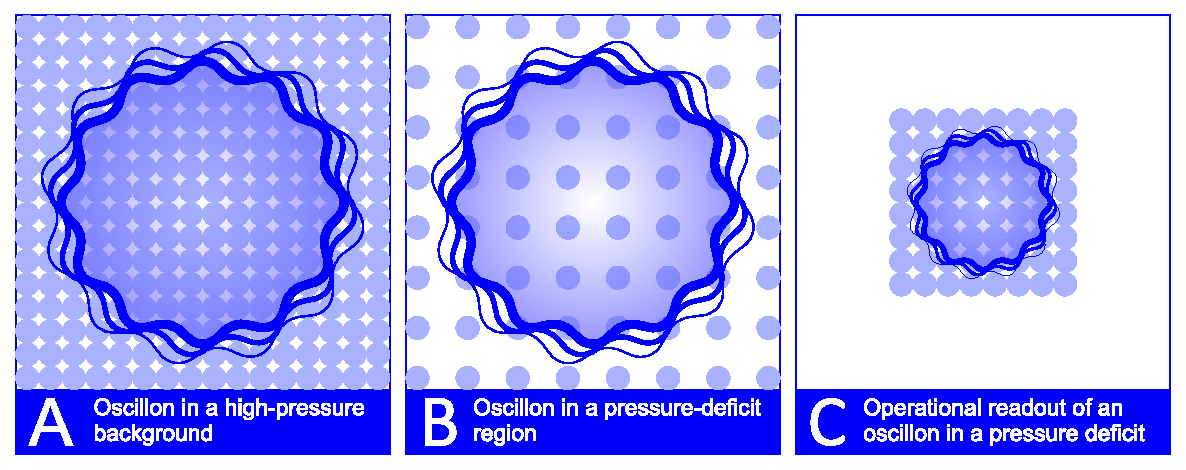
\includegraphics[width=\textwidth]{figures/figure_3.pdf}
\caption{\textbf{სქემატური საილუსტრაციო გამოსახულება: ოსცილონის ოპერაციული ამოკითხვა წნევის დეფიციტის არეში.}
\textbf{(A)} დეფიციტურ არესთან შედარებით უფრო მაღალი წნევის მქონე შეუშფოთებელ ფუძე-გარემოში ოსცილონი შედარებით მკვრივ კვანძურ წყობაში იმყოფება; კვანძებს შორის კავშირი ძლიერია და ლოკალური პროცესები უფრო მაღალი კოორდინატული ტემპით მიმდინარეობს.
\textbf{(B)} წნევის დეფიციტის არეში ფუძის კვანძები გაიშვიათებულია; კვანძთაშორისი ოპერაციული შუალედი იზრდება, გადაცემის ტემპი იკლებს და ლოკალური დროის სვლა ნელდება.
\textbf{(C)} საერთო-მასშტაბური სქემის გარე ამოკითხვაში საათი ნელდება, სახაზავის კოორდინატული კვალი მცირდება და ენერგიის გარე ამოკითხვა იცვლება. ნახაზი ამ სქემატურ თანაფარდობას ასახავს, ხოლო თვითგრავიტირებადი სხეულის ზუსტი ზომა და სრული მასა ერთობლივი საველე განტოლებების ამონახსნიდან განისაზღვრება.}
\label{fig:figure_3_v2}
\end{figure}

\subsection{კვადრატული კავშირი და ფაქტორი 2}

იზოლირებული სისტემის განშტოებაზე, სტატიკურ იზოტროპულ კოორდინატებში, სივრცე-დროის მეტრიკა და ადგილობრივი საზომები შემდეგი სახით ჩაიწერება:

\[
ds^2=-N^2c_0^2dt^2+A_{\rm iso}^2d\boldsymbol{\sigma}^2,\qquad
p_T=N,\quad p_L=A_{\rm iso}^{-1},\quad
d\tau=p_Tdt,\quad d\ell=\frac{d\sigma}{p_L}.
\]

აქ $A_{\rm iso}$ სივრცული მეტრიკული ფაქტორია (რათა იგი გაიმიჯნოს §3.3-ის კოსმოლოგიური მასშტაბისგან $A$). სინათლის ნულოვანი ინტერვალის პირობა ($ds^2 = 0$) იძლევა:

\[
\frac{c_{\rm coord}}{c_0}=p_Tp_L,\qquad
c_{\rm local}=\frac{d\ell}{d\tau}=c_0.
\]

საერთო მეტრიკა მატერიალურ საათს, სახაზავსა და სინათლეს ერთ ადგილობრივ გეომეტრიაში აერთიანებს. ფაქტორები $p_T$ და $p_L$ ზოგად შემთხვევაში დამოუკიდებელი საველე განტოლებებით განისაზღვრება. ასიმპტოტურად ბრტყელ, სუსტ სფეროსიმეტრიულ გარე არეში, უგანზომილებო პოტენციალის $\epsilon=GM/(c_0^2r)$ მიმართ პირველ რიგში, ორივე ფაქტორი ერთმანეთს ემთხვევა: $p_T=1-\epsilon+O(\epsilon^2)$ და $p_L=1-\epsilon+O(\epsilon^2)$. ეს დამთხვევა სუსტი ველის პირველ მიახლოებას ახასიათებს, ხოლო უფრო მაღალ რიგებსა და მატერიის შიგა არეში $p_T$ და $p_L$ დამოუკიდებელ ცვლადებად რჩება.

საერთო-მასშტაბურ ანზაცში სრულდება ზუსტი ტოლობა $p_T=p_L=p$. ამ დროს ადგილობრივი სახაზავის გარე კვალი და საათის კოორდინატული ტაქტი ერთნაირად, $p$ ფაქტორით იცვლება, ხოლო საათის პერიოდი — $p^{-1}$-ით; ამიტომ ამ სპეციალურ განშტოებაზე სინათლის კოორდინატული სიჩქარე $p^2c_0$-ს უდრის.

შესაბამისად, საერთო-მასშტაბურ განშტოებაზე ბიკონფორმული მასშტაბური კანონი ჩაიწერება სახით:

\[
\frac{L_{\rm coord}}{L_0} = \frac{m_{\rm eff}}{m_0} = \frac{\Omega_t}{\Omega_{t,0}} = p, \qquad \frac{c_{\rm coord}}{c_0} = p^2, \qquad p = e^{\varphi/2}.
\]

აქ $L_{\rm coord}$ აღნიშნავს ადგილობრივი სახაზავის კვალს შორეულ, ასიმპტოტურ კოორდინატთა ბადეზე, მაშინ როცა საკუთარ გარემოში დამკვირვებელი მას კვლავ ერთ უცვლელ ერთეულად აღიქვამს. საათის კანონი იძლევა $d\tau=p\,dt$-ს, ხოლო სახაზავის დაკალიბრება — $d\ell=p^{-1}d\sigma$-ს. ამიტომ დროითი მეტრიკული კოეფიციენტი $p^2$-ია, სივრცული — $p^{-2}$, სინათლის კოორდინატული სიჩქარე $p^2c_0$ გამოდის, ხოლო ადგილობრივი საათითა და სახაზავით გაზომილი სინათლის სიჩქარე ზუსტად $c_0$ რჩება.

მსგავსი ხარისხობრივი თანაფარდობა ისტორიულად გვხვდება რობერტ დიკესა და ჰაროლდ პუტჰოფის პოლარიზებადი ვაკუუმის (PV) მოდელებშიც (Dicke 1957; Puthoff 2002). RefG ამ ხარისხებს ფუძის კვანძებისა და მათ შორის კავშირების ონტოლოგიურ გამიჯვნას უკავშირებს.

ფორმალურად, ერთეული ოსცილონის გარედან განსაზღვრული ეფექტური მასა ფუძის წნევითი დეფიციტის პროფილზე $e^{\varphi/2}$ ექსპონენციალური კანონით არის დამოკიდებული:

\[
m_{\rm eff} = m_0 e^{\varphi/2}.
\]

დეფიციტურ განშტოებაზე $\varphi<0$ და $0<p<1$. თანაფარდობა $m_{\rm eff}=pm_0$ წარმოადგენს ფიქსირებული საკუთარი ენერგიის გრავიტაციულად წითლად წანაცვლებული მნიშვნელობის ჩაწერას მასის ერთეულებში. სრული კოფრეიმის სტატიკურ მეტრიკაში სატესტო სხეულის ლაგრანჟიანი იძლევა $L=-mc_0^2N+\tfrac12mA_{\rm iso}^2N^{-1}v^2+O(mv^4/c_0^2)$ გაშლას, საიდანაც ჩანს, რომ გარე მოსვენების ენერგია და კოორდინატული ინერციული კოეფიციენტი განსხვავებული სიდიდეებია. მთელი იზოლირებული სხეულის ფიზიკური ინერცია §2.3-ში სისტემის სრული ენერგია–იმპულსით განისაზღვრება.

ენერგეტიკულ აღრიცხვაში ოთხი ფიზიკური სიდიდე მკაფიოდ უნდა გაიმიჯნოს:

\begin{enumerate}[label=\arabic*.]
\item \textbf{ოსცილონის შინაგანი მდგომარეობა და საკუთარი ენერგია} ($M_{\rm proper}$);
\item \textbf{მოცემულ ფონურ ველში ერთეული ოსცილონის ეფექტური რეფრაქციული მასა} ($m_{\rm eff}$);
\item \textbf{ფუძე-გარემოში შექმნილი წნევითი დეფიციტის წყაროს პროფილი} ($M_{\rm active}$);
\item \textbf{მთელი სისტემის ასიმპტოტური გრავიტაციული მუხტი} (ADM-ისა და კომარის ტიპის სრული მასა: Arnowitt, Deser \& Misner 1962; Komar 1959).

\end{enumerate}
ეს ოთხი სიდიდე აღრიცხვის ორ დონეს ქმნის: პირველ დონეზე ოსცილონის საკუთარი შინაგანი ენერგია განირჩევა მოცემულ გრავიტაციულ გარემოში გარედან წაკითხული წილისგან, ხოლო მეორე დონეზე გარედან გაზომილ სრულ მასაში ერთიანდება აქტიური ბირთვისა და გარემოს წვლილები. ასიმპტოტურ საზღვარზე ისინი ერთ ჯამურ გრავიტაციულ მუხტს აყალიბებს, რომელშიც თითოეული წვლილი მხოლოდ ერთხელ აღირიცხება.

ოსცილონი ერთიანი ფუძის ლოკალიზებული რეზონანსული სტრუქტურაა, თუმცა მისი რეზონანსული გავლენა ბირთვის ფარგლებს სცდება და გარემომცველ ფუძეში ვრცელდება. მრავალი ოსცილონის რეზონანსული ველები ერთმანეთს გადაეფარება, მთელ ფუძე-გარემოს მოიცავს და მის ფონურ წნევას ამცირებს; სწორედ ამ კოლექტიურ პროცესს უკავშირებს RefG სივრცის ფონურ მოდუნებას.

საერთო-$p$ მოდუნების სქემაში რეზონანსული გავლენის არის ზრდა ცვლის ლოკალურ წნევას, გარე ენერგიას, ზომის ამოკითხვას, საათის ტაქტსა და სინათლის კოორდინატულ სიჩქარეს. ამ სქემის უარყოფითი უკუკავშირი და ერთგვაროვანი ასიმპტოტური მოდუნება შესაბამისი სკალარული მოქმედებისა და მდგომარეობის განტოლებების ფარგლებში განიხილება, ხოლო იზოლირებულ კოვარიანტულ სექტორში უკუზემოქმედება $S_{\rm iso}$ მოქმედების ერთობლივი საველე განტოლებებით იმართება.

საერთო-მასშტაბურ $p/p^2$ განშტოებას შეესაბამება შემდეგი ბიკონფორმული მეტრიკა (რომლის ექსპონენციალური ფორმა სრული კოფრეიმის ზოგად ამონახსნთან ცალკე შედარებადი სპეციალური შემთხვევაა):

\[
ds^2 = e^\varphi c^2 dt^2 - e^{-\varphi} d\boldsymbol{\sigma}^2, \qquad \varphi = -\frac{2U}{c^2},
\]

სადაც $U > 0$ არჩეული ექსპონენციალური განშტოების გრავიტაციული პოტენციალია და მთავარ რიგში ნიუტონური პოტენციალის მოდულს ემთხვევა. სუსტი ველის ზღვარში ($U/c^2 \ll 1$) მეტრიკის კომპონენტები ტეილორის მწკრივად იშლება:

\[
g_{00} = e^\varphi \approx 1 - \frac{2U}{c^2} + \frac{2U^2}{c^4} + \cdots, \qquad g_{ij} = -e^{-\varphi}\delta_{ij} \approx -\left(1 + \frac{2U}{c^2} + \cdots\right)\delta_{ij}.
\]

საათისა და სახაზავის საერთო მასშტაბური დამოკიდებულებები განსაზღვრავს ბიკონფორმულ მეტრიკასა და მის პირველ სივრცულ შესწორებას. მასიური წყაროს სტატიკური პროფილი მიიღება ვარიაციული ფუნქციონალიდან სამი პირობით: პასუხი ადიტიური და ლოგარითმულია ($u=-\ln p$), გრადიენტული წევრი კანონიკურია, ხოლო აქტიურ წყაროსთან ბმა წრფივია. ამ პირობებში ფუნქციონალის ვარიაცია და ასიმპტოტური სასაზღვრო პირობა იძლევა ნიუტონურ პროფილს $u=GM/(c^2r)$.

ამ სტატიკურ, სფეროსიმეტრიულ სუსტი ველის აღწერაში მეტრიკის პირველი პოსტნიუტონური (1PN) გაშლა იძლევა პარამეტრიზებული პოსტნიუტონური ფორმალიზმის (PPN) კოეფიციენტებს:

\[
\beta = 1, \qquad \gamma = 1.
\]

აქ $\gamma=1$ საათისა და სახაზავის თანაბარი პირველი რიგის პასუხის გეომეტრიული შედეგია, ხოლო ექსპონენციალური სტატიკური პასუხის მეორე რიგის გაშლა იძლევა $\beta=1$-ს.

ამგვარად, ფუძე-გარემოს თვითრეგულირება აერთიანებს მატერიის მდგომარეობას, წნევით დეფიციტსა და ადგილობრივი საათისა და სახაზავის პასუხს. მათი სრული დინამიკური აღწერა ეფუძნება საერთო გეომეტრიას, რომელშიც მატერიისა და გარემოს თითოეული ენერგეტიკული წვლილი ზუსტად ერთხელ აღირიცხება.

\paragraph{რელაციური კოფრეიმი, აინშტაინ–ჰილბერტის გეომეტრია და სრული 1PN}

ამ ქვეთავის კოვარიანტული განტოლებები ჩაწერილია მეტრიკის $(-+++)$ სიგნატურაში (მაშინ როცა ზემოთ მოყვანილი ბიკონფორმული ჩანაწერი $(+---)$ სიგნატურას იყენებდა).

სტატიკური $p$-პროფილი სრული გეომეტრიის მხოლოდ მოცულობით სკალარულ პროექციას წარმოადგენს. ადგილობრივი გეომეტრიის სრული მდგომარეობა აღიწერება \textbf{რელაციური კოფრეიმით} (თანმხლები ბაზისით) $e^A{}_\mu$ — ადგილობრივი ათვლის სისტემის დიფერენციალურ 1-ფორმათა ნაკრებით, რომელიც აერთიანებს მოცულობას, ფორმას, ძვრას, ორიენტაციასა და დროით მიმართულებას. კოფრეიმი ცალსახად განსაზღვრავს ოპერაციულ მეტრიკას:

\[
g_{\mu\nu}=\eta_{AB}e^A{}_\mu e^B{}_\nu.
\]

კოფრეიმის სივრცე-დროითი ორიენტაცია და ოსცილონის შიდა სამღერძიანი აგებულება განსხვავებული ფიზიკური სტრუქტურებია (ნაწილაკურ რუკაში ფერის კვანტური რიცხვი სწორედ ამ შიდა სამღერძიან სტრუქტურას უკავშირდება). მეზობელი კოფრეიმების შედარება ხორციელდება ბრტყელი, მეტრიკასთან თავსებადი ინერციული კავშირით, ხოლო ელექტრომაგნიტურ არხს საკუთარი $U(1)$ ყალიბური კავშირი აქვს. უსასრულოდ მცირე კონტურის კოფრეიმული გადატანისას წარმოქმნილი დაუხურაობა არის \textbf{გეომეტრიული გრეხა (ტორსია)} — კოფრეიმული უწყვეტი გარემოს არაინტეგრირებადი დეფორმაციის საზომი.

პოსტგენეზისურ რელაციურ-კოფრეიმულ კონტინუუმში წამყვან დაბალენერგიულ მოქმედებას სამი ფიზიკური პირობა განსაზღვრავს:

\begin{enumerate}[label=\arabic*.]
\item მოქმედება არის ლოკალური, დროის შებრუნების მიმართ ინვარიანტული (შექცევადი), მუდმივკოეფიციენტიანი, ლუწი პარიტეტის მქონე და გრეხის (ტორსიის) ტენზორის მიმართ კვადრატული;
\item ფაზური სექტორი გეომეტრიასთან მინიმალურადაა შეწყვილებული და იმავე რიგში დაუთრგუნავი შერეული ოპერატორები არ მონაწილეობს;
\item მინკოვსკის ფონის გარშემო წრფივი ზღვარი რეგულარულია, ხოლო კოფრეიმის ლორენცული ორიენტაცია ინერციულ ყალიბურ თავისუფლებად რჩება — დამოუკიდებელი შორსმწვდომი ფიზიკური ორიენტაციული ტალღა არ აღიძვრება.

\end{enumerate}
ამ პირობებში კვადრატული ინვარიანტების კოეფიციენტთა ერთადერთი დასაშვები თანაფარდობა ზუსტად იძლევა ზოგადი ფარდობითობის ტელეპარალელური ეკვივალენტის (TEGR) კომბინაციას. გრეხის (ტორსიის) სამი დამოუკიდებელი კვადრატული ინვარიანტია:

\[
I_1=T^\rho{}_{\mu\nu}T_\rho{}^{\mu\nu},\qquad
I_2=T^\rho{}_{\mu\nu}T^{\nu\mu}{}_\rho,\qquad
I_3=T_\mu T^\mu,\quad T_\mu=T^\nu{}_{\nu\mu}.
\]

მათი ტელეპარალელური (TEGR) კომბინაცია ტოლია:

\[
T_{\rm TEGR}=\frac14 I_1+\frac12 I_2-I_3.
\]

შესაბამისად, კოსმოლოგიურ ფაზურ განშტოებაზე მოქმედება ჩაიწერება სახით:

\[
S_F=-\frac{c_0^3}{16\pi G}\int d^4x\,e\left(T_{\rm TEGR}+2\Lambda_F\right)
+S_C[g,J,\theta_C]+S_{\partial},
\]

სადაც $S_C$ ფაზური დენის კოვარიანტული მოქმედებაა, ხოლო $S_{\partial}$ — საზღვართან შეწყვილებული წევრი. გრავიტაციული გრეხითი წევრის წინ მდგომი მინუს-ნიშანი ქვემოთ მოყვანილ გრეხა–სიმრუდის იგივეობასთან ერთად ზუსტად აღადგენს აინშტაინ–ჰილბერტის მოქმედების კანონიკურ ნიშანს.

მეტრიკის $(-+++)$ სიგნატურაში სრულდება ზუსტი დიფერენციალურ-გეომეტრიული იგივეობა:

\[
R_{\rm LC}=-T_{\rm TEGR}+\frac{2}{e}\partial_\mu(eT^\mu).
\]

ეს იგივეობა კოფრეიმულ მოქმედებას სრული დივერგენციის (სასაზღვრო წევრის) სიზუსტით გარდაქმნის აინშტაინ–ჰილბერტის მოქმედებად (Beltrán Jiménez \& Dialektopoulos 2020; Maluf 2013). აქ $R_{\rm LC}$ არის ლევი–ჩივიტას კავშირის რიჩის სკალარული სიმრუდე, $e=\det(e^A{}_\mu)$ — კოფრეიმის დეტერმინანტი, ხოლო $T^\mu$ — გრეხის ტენზორის კვალი. მოქმედებათა ეკვივალენტობა ზუსტია კომპაქტური საყრდენის მქონე ვარიაციებისთვის და შესაბამისი ასიმპტოტური კლების პირობებში (ან შეთანხმებული სასაზღვრო წევრის $S_\partial$ გათვალისწინებით). ამგვარად, აინშტაინის გეომეტრია რელაციური კოფრეიმის დაბალენერგიული კონტინუუმური დინამიკის უშუალო გამოვლინებაა. იმავე აინშტაინ–ჰილბერტის ოპერატორამდე მიდის ფიერც–პაულის წრფივი სპინ-2 თეორიისა და დეზერის უნივერსალური თვითბმის დამოუკიდებელი გზაც.

მოქმედება $S_C$ აღწერს ბაროტროპულ, იზენტროპიულ და უგრიგალო ერთპოტენციალურ ფაზურ დენს მის დადებით, მდგრად და მიზეზობრივ მდგომარეობით განშტოებაზე:

\[
\rho_C>0,\qquad \rho_C'>0,\qquad
0\le n_{C,{\rm op}}\rho_C''(n_{C,{\rm op}})/\rho_C'(n_{C,{\rm op}})\le1.
\]

$\theta_C$ ფაზის მიმართ ვარიაცია იძლევა შენახვად დენს, ხოლო მეტრიკის მიმართ ვარიაცია — ჰილბერტის ენერგია–იმპულსის ტენზორს:

\[
T^C_{\mu\nu}=(\rho_C+p_C)u_\mu u_\nu+p_Cg_{\mu\nu}
\]

(Brown 1993). აქ $n_{C,{\rm op}}$ ოპერაციულ მოცულობაზე დათვლილი ფაზური მუხტის სიმკვრივეა, ხოლო $p_C=n_{C,{\rm op}}\rho_C'(n_{C,{\rm op}})-\rho_C(n_{C,{\rm op}})$ — ფაზური სექტორის თერმოდინამიკური წნევა. სიდიდე $P_F$ კი წარმოადგენს ფუძის ფონური წნევის ოპერაციულ ამოკითხვას; ეს ორი სხვადასხვა ფიზიკური ცვლადია და მათი დამაკავშირებელი მდგომარეობის განტოლება ფუძის მიკროფიზიკით განისაზღვრება. მხოლოდ ფაზური დენის წყაროს შემთხვევაში საველე განტოლება იღებს სახეს:

\[
G_{\mu\nu}+\Lambda_Fg_{\mu\nu}=\frac{8\pi G}{c_0^4}T^C_{\mu\nu}.
\]

ზოგად შემთხვევაში გეომეტრიის წყაროა სრული ენერგია–იმპულსის ტენზორი $T^{\rm tot}_{\mu\nu}$, რომელშიც მოქმედების თითოეული ფიზიკური სექტორი საკუთარი მეტრიკული ვარიაციით ზუსტად ერთხელ შედის.

იზოლირებული სისტემის დაბალენერგიული სექტორი ($S_{\rm iso}$) $c_0=\hbar=1$ ერთეულებში ჩაიწერება სახით:

\[
S_{\rm iso}=\int d^4x\sqrt{-g}\left[
\frac{R}{16\pi G}
-g^{\mu\nu}\partial_\mu\Psi_O^*\partial_\nu\Psi_O
-U(|\Psi_O|^2)-\frac14F_{\mu\nu}F^{\mu\nu}
\right]+S_{\partial},\qquad \Lambda=0.
\]

აქ კანონიკური ნორმირებაა $\Psi_O=f e^{i\theta_O}/\sqrt2$ და $U(|\Psi_O|^2)=V(f)$. გამოყენებულ უგანზომილებო ერთეულებში თვითქმედების პოტენციალია $V(f)=f^2/2-f^4/4+f^6/24$, ხოლო მატერიის ლაგრანჟიანი ამპლიტუდა–ფაზის ცვლადებში იღებს $-\tfrac12(\partial f)^2-\tfrac12f^2(\partial\theta_O)^2-V(f)$ ფორმას. $F_{\mu\nu}$ მაქსველის ელექტრომაგნიტური ველის დაძაბულობის ტენზორია. ნეიტრალური ოსცილონის წონასწორობაზე ფონური ელექტრომაგნიტური ველი ნულოვანია, ხოლო სინათლის მცირე აგზნებები იმავე მეტრიკულ სინათლის კონუსზე ვრცელდება. მეტრიკა, მატერიის ველი და მაქსველის ველი დამოუკიდებლად ვარიირდება, კოორდინატთა კონკრეტული სისტემა კი მოძრაობის განტოლებების მიღების შემდეგ შეირჩევა (დამოუკიდებელი სკალარული $u$-ველის დამატება სხვა მოქმედებას შეესაბამება).

თავდაპირველ ჰიდროდინამიკურ ჩანაწერში $S_C[g, J_C, \theta_C]$ კოსმოლოგიური ფაზური სექტორი განსაზღვრული იყო მხოლოდ არანულოვანი სიმკვრივის ($n_{C,{\rm op}} > 0$) არეში: რადგან უძრაობის ქიმიური პოტენციალი დადებითია ($\mu_{C0} = \rho_C'(0) > 0$), ნაკადის განულების ($J_C^\mu \to 0$) ზღვარში წარმოებული $\partial\rho_C/\partial J_C^\mu = \mu_{C0}\,u_{C\,\mu}$ მიმართულებაზეა დამოკიდებული (განიცდის წყვეტას), ხოლო არაერთგვაროვან სტატიკურ გრავიტაციულ ველში ($\nabla_i N \neq 0$) სტაციონარული ფაზა $\theta_C = -\omega_C t$ ეიკონალის ზღურბლურ პირობას $\chi_C \equiv -g^{\mu\nu}\partial_\mu\theta_C\partial_\nu\theta_C = \mu_{C0}^2$ მთელ სივრცეში ერთდროულად ვერ აკმაყოფილებს. ეს ანალიზური წინააღმდეგობა სრულად იხსნება ჰიდროდინამიკური ცვლადების შეცვლით რეგულარული კოლექტიური კომპლექსური სკალარული ველით $\Psi_C = \sqrt{x}\,e^{i\theta_C}$ ($x \equiv |\Psi_C|^2$), რომლის ლაგრანჟიანია:

\[
\mathcal{L}_C(\Psi_C,\nabla\Psi_C,g) = -\frac{1}{2}g^{\mu\nu}\nabla_\mu\Psi_C^*\nabla_\nu\Psi_C - U_C(|\Psi_C|^2), \qquad U_C(x) = \mu_{C0}^2 x + \frac{1}{2}\lambda_C x^2.
\]

ამ გარდაქმნის შედეგად იზოლირებული, კოსმოლოგიური, ძლიერი ველისა და გალაქტიკური სექტორები ერთიანდება ერთ რეგულარულ დიდ კოვარიანტულ მოქმედებაში:

\begin{enumerate}[label=\arabic*.]
\item \textbf{მკაცრი ვაკუუმური რედუქცია ($\Psi_C \equiv 0$, $\Lambda_F = 0$):} რადგან $\mathcal{L}_C$ გლუვი კვადრატული ფუნქციონალია $\Psi_C = 0$ წერტილში, კოლექტიური ველის განულებისას ერთიანი მოქმედება ნებისმიერ გამრუდებულ მეტრიკაზე \textbf{იდენტურად და სინგულარობის გარეშე} გადადის იზოლირებული სისტემის მოქმედებაში $S_{\rm iso}$;
\item \textbf{აქტიური კოსმოლოგიური შტო ($x > 0$):} მაღალსიხშირულ (ტომას–ფერმის, $|\nabla\sqrt{x}|^2 \ll \chi_C x$) რეჟიმში ლეჟანდრის გარდაქმნა $\chi_C = U_C'(x) = \mu_{C0}^2 + \lambda_C x$ ზუსტად აღადგენს ბაროტროპულ ენერგია–იმპულსის ტენზორს $T^C_{\mu\nu} = (\rho_C + p_C)u_\mu u_\nu + p_C g_{\mu\nu}$, სადაც $\rho_C = \mu_{C0}^2 x + \frac{3}{4}\lambda_C x^2$ და $p_C = \frac{1}{4}\lambda_C x^2$, ხოლო განზავებულ ზღვარში ($\lambda_C x \ll \mu_{C0}^2$) იძლევა უწნევო ცივი მტვრის რეჟიმს ($w_C \to 0$, $c_{s,C}^2 \to 0$). თავად ეფექტური პოტენციალის $U_C(|\Psi_C|^2)$ პარამეტრების ($\mu_{C0}, \lambda_C$) გამოყვანა დისკრეტული კვანძების მიკროსკოპული დინამიკიდან შემდგომი კვლევის ამოცანაა;
\item \textbf{ერთიანი დიდი კოვარიანტული მოქმედება და საერთო მასშტაბის სრული დივერგენციის თეორემა:} როდესაც დროითი ფენოვნების (საათის) სკალარი და კოლექტიური კონდენსატის ფაზა ერთმანეთს უკავშირდება იგივეობით $\Phi(x) \equiv -\frac{c_0}{\mu_{C0}}\theta_C(x)$, გარემოს ოთხსიჩქარე $u_\mu = -\partial_\mu\Phi/\sqrt{X} = \partial_\mu\theta_C/\sqrt{\chi_C}$ და მართობული სივრცითი პროექტორი $\gamma^{\mu\nu} = g^{\mu\nu} + u^\mu u^\nu$ ყველა სექტორისთვის იდენტური ხდება. ამასთან, გარემოს დროით-სივრცითი დეფორმაციის ინვარიანტების ($\widehat{Y} \equiv X e^{-2H}/c_0^2$, $\widehat{B}^{AB} \equiv g^{\mu\nu}\partial_\mu\Sigma^A\partial_\nu\Sigma^B e^{2H}$) ენერგეტიკული მასშტაბი და გალაქტიკური გრადიენტული პრეფაქტორი ერთიანდება თანაფარდობით $M_*^4 = \frac{M_{\rm Pl}^2 a_0^2}{2 c_0^4} = \frac{a_0^2}{16\pi G}$. ნებისმიერ სტატიკურ საერთო-მასშტაბურ მეტრიკაზე $ds^2 = -e^{-2H(\mathbf{x})}c_0^2 dt^2 + e^{2H(\mathbf{x})}\delta_{ij}dx^i dx^j$ ($\Phi = c_0 t, \Sigma^A = x^A$) ინვარიანტები $\widehat{Y} \equiv 1$ და $\widehat{B}^{AB} \equiv \delta^{AB}$ იდენტურად სრულდება, ხოლო აინშტაინ–ჰილბერტის სიმრუდისა და კანონიკური ($\omega_H = 1$) პროექციული გრადიენტის ჯამური სიმკვრივე $H(\mathbf{x})$-ის ყველა რიგში \textbf{ზუსტი სრული სივრცითი დივერგენციაა}:
\[
   \sqrt{-g}\left(\tfrac{1}{2}R + \gamma^{\mu\nu}\nabla_\mu H\nabla_\nu H\right) \equiv -\nabla^2 H = -\partial_i(\delta^{ij}\partial_j H), \quad \sqrt{-g}\left(G^t{}_t - \gamma^{\mu\nu}\nabla_\mu H\nabla_\nu H\right) \equiv 2\,\nabla^2 H.
\]
შესაბამისად, სტატიკურ საერთო-მასშტაბურ განშტოებაზე საყრდენი სიმრუდე–გრადიენტის ოპერატორი $H$-ის ველის განტოლებაში მოცულობით წვლილს არ იძლევა და ველი მთლიანად იმართება გარემოს ინვარიანტული მოქმედებით $\mathcal{F}(Z_H/a_0^2)$ ($Z_H = c_0^4\gamma^{\mu\nu}\nabla_\mu H\nabla_\nu H$). კომპაქტური ობიექტების ძლიერ ველში ($r=2m$, $M=1 M_\odot$, სადაც $x_{\rm acc} = |\nabla\Phi|/a_0 \approx 7.69\times 10^{22} \gg 1$) $\mathcal{F}(x^2) \to x^2$ გადასვლის გამო კვადრატული ლაპლასის განტოლებიდან ($\nabla^2 H = 0 \implies H(r) = m/r$) ფარდობითი გადახრა მხოლოდ $1.69\times 10^{-46}$-ია, რაც უზრუნველყოფს ძლიერი ველის უჰორიზონტო ექსპონენციალური მეტრიკისა და გალაქტიკური MOND/RAR რეჟიმის ($x_{\rm acc} \lesssim 1$) სრულ მათემატიკურ თანხმობას ერთ მოქმედებაში.

\end{enumerate}
შერჩეული ტელეპარალელური (TEGR) კოფრეიმული მოქმედება RefG-სა და ზოგად ფარდობითობას ერთსა და იმავე პირველ პოსტნიუტონურ (1PN) ეკვივალენტობის კლასში ათავსებს შემდეგი პირობების შესრულებისას:

\begin{enumerate}[label=\arabic*.]
\item სრული მოქმედება 1PN რიგამდე შედგება აინშტაინ–ჰილბერტის ოპერატორისა და მატერიის მოქმედებისგან;
\item მატერია ერთსა და იმავე მეტრიკას უნივერსალურად და მინიმალურად უკავშირდება;
\item გრავიტაციული წყარო აღირიცხება ერთი სრული, კოვარიანტულად შენახვადი ენერგია–იმპულსის ტენზორით;
\item RefG და ზოგადი ფარდობითობა იყენებს ერთსა და იმავე ლოკალურ წყაროს, PPN ყალიბს, ასიმპტოტურ ფონსა და სასაზღვრო პირობებს;
\item 1PN მიახლოებაში დამატებითი დაუთრგუნავი საველე თავისუფლების ხარისხი ან ოპერატორი არ მონაწილეობს.

\end{enumerate}
ამ პირობებში სრული სტანდარტული PPN პარამეტრების ნაკრებია:

\[
\gamma=\beta=1,\qquad
\xi=\alpha_1=\alpha_2=\alpha_3=\zeta_1=\zeta_2=\zeta_3=\zeta_4=0.
\]

ამ შედეგის მოქმედების არე მოიცავს იზოლირებულ, სუსტ, ნელა მოძრავ და სუსტად თვითგრავიტირებად წყაროებს, რასაც იზოლირებული მოქმედება $S_{\rm iso}$ სრულად აკმაყოფილებს. ექსპონენციალური სტატიკური ანზაცი $\beta=\gamma=1$ თანაფარდობის დამოუკიდებელ შემოწმებას იძლევა, ხოლო მისი მაღალ რიგებში გაგრძელება შესაბამის სკალარულ წყაროსა და მოქმედებაზეა დამოკიდებული.

საათის ერთი სრული ტაქტის ხანგრძლივობა სახაზავის კოორდინატული კვალისა და სინათლის კოორდინატული სიჩქარის შეფარდებითაც გამოისახება: $\Delta t\sim p_L/(c_0p_Tp_L)\propto p_T^{-1}$. ამრიგად, ადგილობრივი სინათლის საათი უშუალოდ აღრიცხავს მეტრიკის დროით კომპონენტს $p_T$. საერთო-მასშტაბური სქემის თვალსაჩინო მაგალითში, როდესაც $p_T=p_L=1/2$, საათის პერიოდი ორმაგდება, ხოლო სინათლის კოორდინატული სიჩქარე ოთხჯერ მცირდება.

სტატიკურ, სფეროსიმეტრიულ ველში $\beta=\gamma=1$ პარამეტრებით განსაზღვრული პირველი პოსტნიუტონური ეფექტები ზუსტად ემთხვევა ზოგადი ფარდობითობის კლასიკურ შედეგებს: სინათლის სხივის გრავიტაციულ გადახრას, შაპიროს რადიოდაყოვნებას, გრავიტაციულ წითელ წანაცვლებასა და პლანეტათა პერიჰელიუმის პრეცესიას (Bertotti, Iess \& Tortora 2003; Will 2014). კერძოდ, კოსმოსურ აპარატ Cassini-ს რადიოკავშირის ექსპერიმენტი $\gamma - 1$ გადახრას $(2.1 \pm 2.3) \times 10^{-5}$ სიზუსტით ზღუდავს.

ისტორიულად, სივრცული მეტრიკული კომპონენტის $g_{ij}$ გათვალისწინებით მიღებულმა \textbf{ფაქტორმა 2} აინშტაინის 1911 წლის ნახევარი გადახრის პროგნოზი 1915–1916 წლების სრული გეომეტრიული შედეგით შეცვალა (Einstein 1916; Shapiro 1964). RefG-ის სუსტ იზოტროპულ გარე არეში საათისა და სახაზავის პირველი რიგის პასუხები ერთმანეთის ტოლია, ხოლო მათი ნამრავლი სინათლის კოორდინატულ სიჩქარეში ორივე წვლილს ბუნებრივად აერთიანებს.


\subsection{რეფრაქციული მიზიდულობა, ინერცია და ხახუნის არარსებობა}

ოსცილონი, როგორც სივრცულად განფენილი ტალღური სტრუქტურა, ვრცელდება ფუძე-გარემოს წნევისა და კოორდინატული ტალღური სიჩქარის სივრცით გრადიენტებში. მის უფრო მკვრივ მხარეს ფაზური სიჩქარე მაღალია, ხოლო გაიშვიათებულ (დეფიციტურ) მხარეს — დაბალი. ამ სხვაობის გამო, ჰიუგენს–ფრენელის პრინციპისა და ეიკონალის განტოლების თანახმად, ტალღური ფრონტი დაბალი წნევისა და შემცირებული კოორდინატული სიჩქარის არისკენ იხრება — ანუ განიცდის \textbf{რეფრაქციას (გარდატეხას)}. სუსტ, სტატიკურ ზღვარში მასიური სხეულის მიერ შექმნილი წნევითი დეფიციტი ეფექტურ ოპტიკურ-გეომეტრიულ გარემოს აყალიბებს, ხოლო ამ გარემოში მატერიის ტალღური პაკეტის გარდატეხილი ტრაექტორია მაკროსკოპულ დონეზე გრავიტაციულ მიზიდულობად ვლინდება.

RefG-ის მიხედვით, დედამიწის გრავიტაციულ ველში სხეულის თავისუფალი ვარდნა მისი შემადგენელი ატომების ოსცილონური სტრუქტურების რეფრაქციული გადახრის შედეგია. ეს გადახრა მიმართულია დედამიწის მიერ შექმნილი დაბალი წნევისა და ნელი კოორდინატული გავრცელების არისკენ. ამგვარად, გრავიტაციული მიზიდულობა გარემოს სივრცით არაერთგვაროვნებაზე ტალღური მატერიის უშუალო ლოკალური პასუხია.

რელაციურ-კოფრეიმულ აღწერაში ფუძის დეფორმაცია სრული ტენზორული გეომეტრიით აღირიცხება. მისი სტატიკური საათობრივი და სივრცული მახასიათებლებია $p_T$ და $p_L$, ხოლო სუსტი გარე ველის საერთო-$p$ მიახლოება კლასიკურ რეფრაქციულ სურათს აღადგენს. იზოლირებულ მოქმედებაში $S_{\rm iso}$ კანონიკური მატერია და მაქსველის ველი ჰილბერტის ენერგია–იმპულსის ტენზორში საკუთარი მეტრიკული ვარიაციით ერთხელ შედის. შეკრული სისტემის სრული ასიმპტოტური მასა აერთიანებს მატერიის საკუთარ ენერგიასა და გრავიტაციულ ბმას; დადებითი $B$ ბმის ენერგიის მქონე სისტემისთვის მასის დეფექტია $\Delta M=B/c_0^2$.

გრავიტაციულ-ტალღური მოვლენა GW150914 ამ ენერგეტიკული ბალანსის უშუალო დაკვირვებითი მაგალითია: საწყისი ორმაგი სისტემისა და შერწყმის შედეგად მიღებული სხეულის ასიმპტოტურ მასებს შორის დაახლოებით სამი მზის მასის ($3 M_\odot$) ტოლი სხვაობა გრავიტაციული ტალღების ენერგიის სახით გამოსხივდა (Abbott et al. 2016). RefG-ის ენაზე, ორი მერყევი წყარო ერთ უფრო ღრმა დეფიციტურ პროფილად გადაეწყობა, ხოლო ტელეპარალელურ (TEGR) დაბალენერგიულ გეომეტრიაში ეს სწრაფი არაწრფივი გადაწყობა აღიწერება სტანდარტული განივ-უკვალო ტენზორული ტალღების გამოსხივებით.

RefG-ის დაბალენერგიულ კოვარიანტულ განშტოებაზე სხეულის \textbf{ინერციას} განსაზღვრავს ოსცილონისა და მისი საკუთარი გრავიტაციული ველის სრული ენერგია–იმპულსი. სხეულის თანაბარი და წრფივი მოძრაობა მიიღება მთელი სტაციონარული ამონახსნის ლორენცის გარდაქმნით, რომლის დროსაც მატერიის ფაზა, სივრცული პროფილი და გარემომცველი გეომეტრია შეთანხმებულად გარდაიქმნება. აჩქარებისას გარე ძალა სწორედ ამ ერთიანი სისტემის სრულ იმპულსს ცვლის. ფუძის დეფიციტური პროფილის ასიმეტრიული გადაწყობა ამ პროცესის ინტუიციური ფიზიკური სურათია, ხოლო მისი კვანძური დაყოვნების დეტალური მექანიზმი ფუძის მიკროსკოპულ დინამიკას ეკუთვნის.

იზოლირებული, სივრცულად ლოკალიზებული ამონახსნისთვის მკაცრად სრულდება რელატივისტური დისპერსიული და ინერციული თანაფარდობები:

\[
E(v)=\gamma E_0,\qquad
\mathbf P(v)=\gamma\frac{E_0}{c_0^2}\mathbf v,\qquad
M_I=\left.\frac{\partial P_\parallel}{\partial v}\right|_{v=0}
=\frac{E_0}{c_0^2}.
\]

ბრტყელ სივრცე-დროში ეს ტოლობა უშუალოდ გამომდინარეობს მატერიის სრული ძაბვის ტენზორიდან და ლაუეს წონასწორობის იგივეობიდან ($\int T^{ij}d^3x=0$), ხოლო თვითგრავიტირებადი სხეულის შემთხვევაში $E_0$ არის სისტემის სრული ასიმპტოტური (ADM) ენერგია და იმპულსიც სრული მეტრიკის ასიმპტოტური ინტეგრალით განისაზღვრება. თანაბარი მოძრაობისას სხეულის მოსვენების მასა $E_0/c_0^2$ ინვარიანტულია, სრული ენერგია კი $\gamma E_0$-მდე იზრდება, ხოლო სიგრძის ლორენცული შემოკლება მოძრაობის მიმართულებით კოორდინატულ ამოკითხვას ასახავს. სუსტ, ნელა ცვალებად გარე გრავიტაციულ ველში მონოპოლურ რიგამდე აქტიური და პასიური გრავიტაციული მასებიც ზუსტად $E_0/c_0^2$-ს უდრის (სწრაფი შიდა დეფორმაცია, მოქცევითი ძალები და გამოსხივებითი უკურეაქცია მაღალი რიგის შესწორებებს წარმოადგენს). კოსმოსური მისია MICROSCOPE-ის შედეგი სუსტი ეკვივალენტობის პრინციპის უმკაცრესი დაკვირვებითი საზომია (Touboul et al. 2022).

თანაბარი და წრფივი მოძრაობისას ოსცილონის ტალღური სტრუქტურა ფუძის კვანძებს შორის სიმეტრიულად, ენერგიის გაბნევის (დისიპაციის) გარეშე გადაიცემა. RefG \textbf{უხახუნო მოძრაობას (ინერციით მოძრაობას)} სწორედ ამ კოჰერენტული ფაზური გადაცემის რეჟიმს უკავშირებს: სხეულის გადაადგილება კვანძოვან გარემოში მისი ტალღური მდგომარეობის თანმიმდევრული გადაცემით ხორციელდება. დაბალენერგიულ უწყვეტ (კონტინუუმურ) ზღვარში საერთო ლორენცული სტრუქტურა ფაზური გადაცემის ზღვრულ სიჩქარეს უშუალოდ მეტრიკულ სინათლის კონუსთან აიგივებს.

ამავე მოქმედებაში გამოთვლილი სუსტად ბმული ოსცილონის წონასწორობა დადასტურებულია ვარიაციული ენერგეტიკული შემოწმებითაც: სრული ფაზური მუხტის ფიქსირებისას პროფილის რადიალური დეფორმაცია ყველა შესწავლილ მიმართულებაში ზრდის სისტემის სრულ ენერგიას, რაც გამოთვლითი ბადის დახვეწისა და გარე საზღვრის გაზრდისას მდგრადად ნარჩუნდება. ეს ადასტურებს სხეულის რადიალურ მდგრადობას, ხოლო სრული სამგანზომილებიანი არაწრფივი ევოლუციის კვლევა შემდგომი რიცხვითი ამოცანაა.

როდესაც ოსცილონი განიხილება ერთიან კოვარიანტულ მოქმედებაში გარემოს კოლექტიურ $\Psi_C$ ველთან ერთად, ვლინდება გარემოსთან შეწყვილების სამი მკაცრი ფიზიკური რეჟიმი:

\begin{enumerate}[label=\arabic*.]
\item \textbf{უსასრულო რეზერვუარის $1/r$ განშლადობის თეორემა:} ასიმპტოტურად ბრტყელ უსასრულო სივრცეში გლობალური სიხშირის $\omega_C \ge \mu_{C0}$ შენარჩუნება შეუძლებელია, რადგან ოსცილონის გრავიტაციული წითელი წანაცვლების ($N(r) \simeq 1 - GM/r < 1$) გამო ლოკალური ქიმიური პოტენციალი $\omega_C/N(r)$ შორ მანძილებზე აჭარბებს ზღურბლურ მნიშვნელობას $\mu_{C0}$; ეს წარმოშობს $\Psi_C$ ველის $1/r$ ასიმპტოტურ კუდს და იწვევს სრული მუხტისა და მასის კვადრატულ განშლადობას ($Q_C(R), M_C(R) \propto R^2 \to \infty$);
\item \textbf{სუფთა ვაკუუმისა და „გრავიტაციულად დაჭერილი ჯიბის“ რეჟიმები:} როდესაც $\omega_C \le \mu_{C0} N_0(0)$, გარემოს კოლექტიური ველი საერთოდ არ აღიძვრება ($\Psi_C \equiv 0$) და იზოლირებული ოსცილონის ყველა თვისება უცვლელი რჩება; ხოლო შუალედურ სიხშირულ ფანჯარაში $\mu_{C0} N_0(0) < \omega_C < \mu_{C0}$ კოლექტიური ველი $\Psi_C$ კონდენსირდება უშუალოდ ნაწილაკის გრავიტაციულ პოტენციალურ ჭაში, სასრული რადიუსის ($r < r_{\rm trap}(\omega_C)$) კომპაქტურ „დაჭერილ ჯიბეში“;
\item \textbf{ორმუხტიანი პირველი კანონი და შედგენილი სხეულის ინერცია:} დაჭერილი ჯიბის რეჟიმში სისტემა ემორჩილება ზუსტ ორმუხტიან ვარიაციულ პირველ კანონს:

\[
dM_{\rm ADM} = \Omega\,dQ + \omega_C\,dQ_C.
\]

\end{enumerate}
რადგან ორივე ველი ($\Psi_O$ და $\Psi_C$) სასრულ არეშია ლოკალიზებული და გარე სივრცე ასიმპტოტურად ბრტყელია, შედგენილი $(Q, Q_C)$ სხეულის ინერციული მასა კვლავ \textbf{ზუსტად} უდრის მის სრულ გრავიტაციულ ენერგიას: $M_I = M_{\rm ADM}(Q, Q_C)$. არანულოვან, უსასრულოდ განფენილ კოსმოლოგიურ ფონში ($\Psi_C(\infty) \neq 0$) სხეულის მოძრაობისას ჰიდროდინამიკური თანდართული მასისა და სასრული არის სასაზღვრო ეფექტების გამოთვლა ცალკე კვლევითი ამოცანაა.


\subsection{ლოკალური შეუმჩნევლობა და ფარდობითობის პრინციპი}

გრავიტაციულ ველში მყოფი ადგილობრივი დამკვირვებელი დროსა და სივრცულ ზომებს იმავე მეტრიკის ორთონორმირებულ ათვლის სისტემაში (ბაზისში) ზომავს, რომელთანაც მატერია და სინათლეა შეწყვილებული. ამიტომ ადგილობრივად გაზომილი სინათლის სიჩქარე ყოველთვის $c_0$-ის ტოლია, მიუხედავად იმისა, რომ საათისა და სახაზავის კოორდინატული ფაქტორები ($p_T$ და $p_L$) იცვლება. შინაგან რხევით პერიოდებთან შედარებით გარემოს ნელი ცვლილება ადიაბატურ რეჟიმში მიმდინარეობს, ხოლო კონკრეტული მატერიალური სპექტრისა და უგანზომილებო ფარდობების პასუხი შესაბამისი მოქმედებიდან და მცირე შეშფოთებების განტოლებიდან განისაზღვრება. საერთო-მასშტაბური სურათი ამ ლოკალურ თვითდაკალიბრებას $p_T=p_L$ სპეციალურ შემთხვევაში აღწერს.

ამ მექანიზმის დაკვირვებით საზღვრებს ორი კლასის ექსპერიმენტი ადგენს:

\begin{itemize}
\item \textbf{გრავიტაციული წითელი წანაცვლება:} პაუნდ–რებკას ცდა (Pound \& Rebka 1960), Gravity Probe A-ს წყალბადის მაზერით ჩატარებული ექსპერიმენტი (Vessot et al. 1980) და Galileo-ს თანამგზავრული გაზომვები (Delva et al. 2018; Herrmann et al. 2018) მაღალი სიზუსტით ადასტურებს საათის სვლის დამოკიდებულებას გრავიტაციულ პოტენციალზე. RefG ამ დამოკიდებულებას საერთო წნევით-გეომეტრიული პასუხის დროით კომპონენტად განიხილავს.
\item \textbf{უგანზომილებო ფარდობების ინვარიანტობა:} შორეული კვაზარების შთანთქმის სპექტრები და ლაბორატორიული ოპტიკური ატომური საათები ნაზი სტრუქტურის მუდმივის ($\alpha$) შესაძლო ცვლილებას კოსმოლოგიურ დროში $|\Delta\alpha/\alpha| \lesssim 10^{-6}$ დონეზე ზღუდავს (Kotuš et al. 2017), რაც სრულად შეესაბამება საერთო-ტაქტური თვითდაკალიბრების პრინციპს.

\end{itemize}
მაიკელსონ–მორლის ექსპერიმენტის ნულოვანი შედეგი ასახავს გარემოს \textbf{საერთო-რეჟიმულ თვითდაკალიბრებას}, ხოლო გრავიტაციულ-ტალღური დეტექტორების (LIGO, Virgo, KAGRA) მიერ რეგისტრირებული სიგნალები — \textbf{დიფერენციალურ ტენზორულ პასუხს}:

\begin{itemize}
\item ადგილობრივი საათი, სახაზავი და სინათლის სიგნალი ერთი და იმავე მეტრიკის ათვლის სისტემაში კალიბრდება. თანამედროვე ოპტიკური რეზონატორები სინათლის სიჩქარის ადგილობრივ მიმართულებით ანიზოტროპიას $\Delta c/c\lesssim10^{-17}$ დონეზე ზღუდავს (Herrmann et al. 2009).
\item გრავიტაციული ტალღა წარმოადგენს დროში ცვლად, კვადრუპოლურ დიფერენციალურ დეფორმაციას ($h_+,h_\times$): იგი სივრცის ერთ ღერძს ჭიმავს, მის მართობულ ღერძს კი კუმშავს. ეს საპირისპირო ნიშნის დეფორმაცია არღვევს საერთო-რეჟიმულ კომპენსაციას და ინტერფერომეტრის მართობულ მკლავებს შორის გაზომვად ფაზურ წანაცვლებას წარმოშობს.

\end{itemize}
ფიცჯერალდ–ლორენცის სიგრძის შემოკლება (FitzGerald 1889; Lorentz 1892) ამ ლოგიკის ისტორიული წინამორბედია. RefG ამ მოვლენას ხსნის იმით, რომ თავად საზომი ხელსაწყოები ფუძე-გარემოს ტალღური აგზნებებისგან არის აგებული.

ტელეპარალელურ (TEGR) დაბალენერგიულ გეომეტრიაში გრავიტაციული ტენზორული ტალღა საერთო მეტრიკული სინათლის კონუსით ვრცელდება, ამიტომ წამყვან რიგში $v_{\rm gw}=c$. ნეიტრონული ვარსკვლავების შერწყმის მოვლენაზე (GW170817) გრავიტაციული და გამა-გამოსხივების სიგნალების თითქმის ერთდროულმა რეგისტრაციამ მათი სიჩქარეების ფარდობითი სხვაობისთვის დაადგინა უმკაცრესი საზღვრები:

\[
-3 \times 10^{-15} \le \frac{v_{\rm gw} - c}{c} \le +7 \times 10^{-16}
\]

(Abbott et al. 2017). ამავე დროს, რელატივისტური ორმაგი პულსარების (PSR B1913+16, PSR J0737-3039A/B) ორბიტული პერიოდის კლება $10^{-3}$–$10^{-4}$ სიზუსტით ადასტურებს კვადრუპოლური გამოსხივების ზოგად-ფარდობითობით ფორმულას (Weisberg \& Huang 2016; Kramer et al. 2021), ხოლო სკალარული („სუნთქვითი“) პოლარიზაციის შესაძლო წილს მკაცრად ზღუდავს LIGO-Virgo-KAGRA-ს GWTC-3 კატალოგი (LIGO Scientific Collaboration, Virgo Collaboration \& KAGRA Collaboration 2022).

RefG-ის ერთიანი დიდი კოვარიანტული მოქმედების იზოლირებულ შტოზე ($\Psi_C \equiv 0$, $\Lambda_F = 0$) ეს მთელი გრავიტაციულ-ტალღური სექტორი მკაცრად და პარამეტრების გარეშე იკეტება:

\begin{enumerate}[label=\arabic*.]
\item \textbf{კოფრეიმის წრფივი გაშლა, $v_{\rm gw} \equiv c_0$ და 2 განივ-უკვალო ($h_+, h_\times$) პოლარიზაცია:} მინკოვსკის ფონის გარშემო რელაციური კოფრეიმის გაშლა $e^A{}_\mu = \delta^A_\mu + \frac{1}{2}\eta^{AB}h_{B\mu} + \frac{1}{2}\eta^{AB}\omega_{B\mu}$ ($h_{\mu\nu} = h_{\nu\mu}, \omega_{\mu\nu} = -\omega_{\nu\mu}$) იძლევა პირველი რიგის მეტრიკულ შეშფოთებას $g^{(1)}_{\mu\nu} = h_{\mu\nu}$, რომელიც იგივურად დამოუკიდებელია ანტისიმეტრიული ლოკალური ლორენცის ორიენტაციის 6 მოდისგან ($\partial g^{(1)}_{\mu\nu}/\partial\omega_{\alpha\beta} \equiv 0$). კვალშებრუნებული ტენზორისთვის $\bar{h}_{\mu\nu} \equiv h_{\mu\nu} - \frac{1}{2}\eta_{\mu\nu}h$ წრფივი აინშტაინის ტენზორი $G^{(1)}_{\mu\nu}$ იგივურად აკმაყოფილებს ბიანკის იგივეობას $\partial^\mu G^{(1)}_{\mu\nu} \equiv 0$, ხოლო ლორენცის ყალიბში ($\partial^\mu\bar{h}_{\mu\nu} = 0$) გადადის ზუსტ ტალღურ განტოლებაში:
\[
   \Box\bar{h}_{\mu\nu} = \left(-\frac{1}{c_0^2}\frac{\partial^2}{\partial t^2} + \nabla^2\right)\bar{h}_{\mu\nu} = -\frac{16\pi G}{c_0^4}T_{\mu\nu}, \qquad v_{\rm phase} = v_{\rm group} = c_0 \implies \frac{v_{\rm gw}^{\rm RefG} - c_0}{c_0} \equiv 0.
\]
სიმეტრიული ტენზორის $10$ კომპონენტიდან $4$ ლორენცის პირობისა და $4$ ნარჩენი ჰარმონიული ყალიბური გარდაქმნის გამოკლებით რჩება ზუსტად \textbf{$10 - 4 - 4 = 2$} ორთოგონალური განივ-უკვალო პოლარიზაცია ($h_+, h_\times$: $\eta^{\mu\nu}e^{+,\times}_{\mu\nu} = 0$, $k^\mu e^{+,\times}_{\mu\nu} = 0$, $e^+_{\mu\nu}e^{+\mu\nu} = e^\times_{\mu\nu}e^{\times\mu\nu} = 2$, $e^+_{\mu\nu}e^{\times\mu\nu} = 0$) ნულოვანი სკალარული ან ვექტორული გამოსხივებითი მოდებით. მაშინ როცა იზოტროპული სკალარული საათ–სახაზავის წანაცვლება ($\delta p_T = \delta p_L = \delta p$) მაიკელსონის ინტერფერომეტრის მართობულ მკლავებში იგივურად ბათილდება ($\Delta\tau_x - \Delta\tau_y \equiv 0$), განივ-უკვალო ტალღა იძლევა დიფერენციალურ სიგნალს $(\Delta L_x - \Delta L_y)/L_0 = h_+\cos(2\psi) + h_\times\sin(2\psi)$.
\item \textbf{აისაქსონის ნაკადი, პეტერს–მათიუსის $f(e), g(e)$ ფაქტორები და დიპოლური გამოსხივების არარსებობა:} აისაქსონის ეფექტური ტენზორის $t^{\rm GW}_{\mu\nu} = \frac{c_0^4}{32\pi G}\langle\partial_\mu h^{\rm TT}_{ij}\partial_\nu h^{\rm TT\,ij}\rangle$ სფერულ კუთხეზე ინტეგრირება ($\langle\Lambda_{ij,kl}Q_{ij}Q_{kl}\rangle_{S^2} = \frac{2}{5}Q_{ij}Q^{ij}$) იძლევა აინშტაინის კვადრუპოლურ ფორმულას $P_{\rm GW} = \frac{G}{5 c_0^5}\langle\dddot{Q}_{ij}\dddot{Q}^{ij}\rangle$. კეპლერის ელიფსურ ორბიტაზე ($r(\theta) = \frac{a(1-e^2)}{1+e\cos\theta}$) სიმბოლური გასაშუალება იძლევა პეტერს–მათიუსის ენერგიისა და კუთხური მომენტის ფაქტორებსა და ორბიტალური პერიოდის კლების კანონს:
\[
   \dot{P}_b^{\rm RefG} = -\frac{192\pi}{5}\left(\frac{2\pi G\mathcal{M}_c}{c_0^3 P_b}\right)^{5/3} f(e), \qquad
   f(e) = \frac{1 + \frac{73}{24}e^2 + \frac{37}{96}e^4}{(1 - e^2)^{7/2}}, \qquad
   g(e) = \frac{1 + \frac{7}{8}e^2}{(1 - e^2)^2},
\]
და პეტერსის ზუსტ ორბიტალურ ინვარიანტს $c_0(a,e) = a(1-e^2)e^{-12/19}[1 + \frac{121}{304}e^2]^{-870/2299}$ ($\frac{d}{dt}\ln c_0(a,e) \equiv 0$). რადგან იზოლირებულ შტოზე ყველა თვითგრავიტირებადი სხეულისთვის სრულდება $M_I = M_A = M_P = M_{\rm ADM}$, სკალარული მგრძნობელობების სხვაობა იგივურად ნულია ($\Delta s_{12} = 0$) და მონოპოლური/დიპოლური გამოსხივება არ არსებობს ($\dot{P}_b^{\rm dipole} \equiv 0$).
\item \textbf{რელატივისტური ორმაგი პულსარების (\texttt{PSR B1913+16}, \texttt{PSR J0737-3039A/B}, \texttt{PSR J1738+0333}) და კოსმოლოგიური სტანდარტული სირენების შემოწმება:}
\begin{itemize}
\item \textbf{ჰალს–ტეილორის პულსარი PSR B1913+16} ($P_b = 0.32299745\text{ დღე}$, $e = 0.6171340$, $m_1 = 1.438\,M_\odot, m_2 = 1.390\,M_\odot$): ექსცენტრიულობის ფაქტორია $f(e) = 11.8568$, შეერთების დრო $T_{\rm coal} = 300.70\text{ მლნ წ.}$ (\texttt{DOP853} და ანალიზური ინტეგრალი ემთხვევა $3.58\times 10^{-15}$ სიზუსტით), ხოლო ორბიტალური პერიოდის კლებაა \textbf{$\dot{P}_b^{\rm RefG} = -2.4021\times 10^{-12}\text{ წმ/წმ}$}, რაც ემთხვევა დაკვირვებით მნიშვნელობას $\dot{P}_b^{\rm int,obs} = (-2.398 \pm 0.004)\times 10^{-12}\text{ წმ/წმ}$ ($\text{obs}/\text{RefG} = 0.9983 \pm 0.0017$, \textbf{$1.03\sigma$}; Weisberg \& Huang 2016).
\item \textbf{ორმაგი პულსარი PSR J0737-3039A/B} ($P_b = 0.10225156\text{ დღე}$, $e = 0.0877770$, $m_A = 1.338185\,M_\odot, m_B = 1.248868\,M_\odot$, $f(e) = 1.0515$): მიიღება \textbf{$\dot{P}_b^{\rm RefG} = -1.247810\times 10^{-12}\text{ წმ/წმ}$}, რაც 16-წლიან დაკვირვებას $\dot{P}_b^{\rm int,obs} = (-1.247752 \pm 0.000079)\times 10^{-12}\text{ წმ/წმ}$ ემთხვევა \textbf{$4.68\times 10^{-5}$ ფარდობითი სიზუსტით ($0.74\sigma$)} (Kramer et al. 2021), ამავე $(m_A, m_B)$ წერტილში დანარჩენი 4 პოსტ-კეპლერული პარამეტრის ($\dot{\omega}^{\rm 1PN} = 16.8994^\circ/\text{წ}$, $\gamma_E = 0.38400\text{ მწმ}$ [$0.51\sigma$], $r_{\rm Sh} = 6.151\,\mu\text{წმ}$ [$0.51\sigma$], $s_{\rm Sh} = \sin i = 0.99992$) ერთდროული თანაკვეთით.
\item \textbf{პულსარ–თეთრი ჯუჯის ასიმეტრიული წყვილი PSR J1738+0333} ($m_p = 1.47\,M_\odot, m_c = 0.181\,M_\odot$): $\dot{P}_b^{\rm RefG} = -2.759\times 10^{-14}\text{ წმ/წმ}$ vs. $(-2.59 \pm 0.32)\times 10^{-14}\text{ წმ/წმ}$ (\textbf{$0.53\sigma$}; Freire et al. 2012), რაც გამორიცხავს ანომალურ დიპოლურ გამოსხივებას.
\item \textbf{კოსმოლოგიური გავრცელება:} ოპერაციულ $A = a/p = a^{5/2}$ გეომეტრიაზე კანონიკური ტენზორული ამპლიტუდა $\chi_k = A\,h_k$ აკმაყოფილებს $\chi_k'' + (k^2 - A''/A)\chi_k = 0$ განტოლებას ($\alpha_M \equiv 0$), რის გამოც გრავიტაციულ-ტალღური და ელექტრომაგნიტური ფuminosity მანძილები იგივურად ტოლია: \textbf{$D_L^{\rm GW}(z) \equiv D_L^{\rm EM}(z) = (1+z)D_M(z)$}.

\end{itemize}
\end{enumerate}
მეტრიკის $(-+++)$ სიგნატურაში ამ აღწერის უშუალო ოპერაციული ინვარიანტია სხვადასხვა გრავიტაციულ პოტენციალსა და სიჩქარეობრივ მსოფლიო წირზე მოძრავი ორი საათის მიერ აღრიცხული საკუთარი დროების სხვაობა:

\[
\tau_a=\frac{1}{c}\int_{\gamma_a}\sqrt{-g_{\mu\nu}dx^\mu dx^\nu},
\qquad
\Delta\tau=\tau_1-\tau_2.
\]

საათების მიერ დაგროვილი საკუთარი დროები სხვადასხვა წნევით რეჟიმში მათი მოძრაობის ისტორიის ინვარიანტული შედეგია, მაშინ როცა თითოეული დამკვირვებლის მიერ საკუთარ ათვლის სისტემაში გაზომილი მყისიერი ტემპი და ზომა საერთო გარემოს ადგილობრივი ფარდობითი მახასიათებლებია.


\subsection{ისტორიული კონტექსტი და RefG-ის ადგილი}

გრავიტაციის რეფრაქციული (ოპტიკურ-გარემოსეული) აღწერა ზოგადი ფარდობითობის ჩამოყალიბების ეპოქიდანვე განიხილება. 1911–1912 წლებში, საბოლოო ტენზორულ ფორმულირებამდე, ალბერტ აინშტაინი სინათლის კოორდინატულ სიჩქარეს გრავიტაციულ პოტენციალს შემდეგი თანაფარდობით უკავშირებდა:

\[
c(\Phi) = c_0 \left(1 + \frac{\Phi}{c^2}\right)
\]

(Einstein 1911, 1912). მოძრავი გარემოს ოპტიკური თვისებების კვლევას კიდევ უფრო ხანგრძლივი ისტორია აქვს: 1851 წელს არმან იპოლიტ ფიზომ ექსპერიმენტულად აღმოაჩინა მოძრავ წყალში სინათლის ნაწილობრივი ჩათრევის ეფექტი (ფრენელის ჩათრევის კოეფიციენტით: Fizeau 1851). 1923 წელს ვალტერ გორდონმა დაამტკიცა, რომ მოძრავ დიელექტრიკულ გარემოში ელექტრომაგნიტური ტალღების გავრცელება აღიწერება ეფექტური ლორენცული (ფსევდორიმანული) მეტრიკის ნულოვანი გეოდეზიური წირებით (Gordon 1923), რითაც პირველად დამყარდა მკაცრი მათემატიკური კავშირი გარემოს ოპტიკასა და სივრცე-დროის გეომეტრიას შორის.

1957 წელს რობერტ დიკემ გრავიტაცია აღწერა ვაკუუმის ცვლადი გარდატეხის მაჩვენებლით (Dicke 1957). თანამედროვე \textbf{ანალოგური გრავიტაციის} მიმართულებას საფუძველი ჩაუყარა უილიამ უნრუს 1981 წლის ნაშრომმა, რომელშიც ნაჩვენებია, რომ მოძრავ ზებგერით სითხეში აკუსტიკური ტალღების გავრცელება შავი ხვრელის აკუსტიკური ჰორიზონტის მქონე ეფექტური მეტრიკით აღიწერება (Unruh 1981).

გრიგორი ვოლოვიკის კონდენსირებული გარემოს პროგრამამ (Volovik 2003) და ბარსელო–ლიბერატი–ვისერის მიმოხილვამ (Barceló, Liberati \& Visser 2011) აჩვენა, თუ როგორ შეიძლება წარმოიშვას ლოკალური ლორენც-ინვარიანტობა და ეფექტური გამრუდებული სივრცე-დრო ფონური კვანტური კონდენსატის (მაგალითად, ზედენადი ჰელიუმ-3-ისა და ჰელიუმ-4-ის) მიკროსკოპული დინამიკიდან. 2019 წელს ჯეფ შტაინჰაუერის ჯგუფმა რუბიდიუმის ბოზე–აინშტაინის კონდენსატში ექსპერიმენტულად დააფიქსირა ჰოკინგის კვანტური თერმული გამოსხივების აკუსტიკური ანალოგი (Muñoz de Nova et al. 2019).

პარალელურად განვითარდა გრავიტაციის \textbf{თერმოდინამიკური და ენტროპიული წარმოშობის} კვლევები:

\begin{itemize}
\item ანდრეი სახაროვმა გრავიტაცია ვაკუუმის კვანტური ფლუქტუაციებიდან წარმოქმნილ დრეკად პასუხად განიხილა (Sakharov 1967);
\item ტედ იაკობსონმა აჩვენა, რომ ლოკალური რინდლერის ჰორიზონტების თერმოდინამიკური ბალანსიდან ($\delta Q = T dS$) აინშტაინის საველე განტოლებები უშუალოდ მდგომარეობის განტოლების სახით მიიღება (Jacobson 1995);
\item ერიკ ვერლინდემ გრავიტაციული მიზიდულობა ჰოლოგრაფიულ ეკრანებზე ინფორმაციის ცვლილებით გამოწვეულ ენტროპიულ ძალად წარმოადგინა (Verlinde 2011).

\end{itemize}
ყველა ამ მიმართულებასა და RefG-ს აერთიანებს ფუნდამენტური იდეა, რომ სივრცე-დროის გეომეტრია წარმოებული ფიზიკური სტრუქტურაა. RefG ამ გეომეტრიის წყაროდ განიხილავს უნივერსალურ წნევით-რეფრაქციულ ფუძე-გარემოს და აერთიანებს ოთხ ძირითად პრინციპს:

\begin{enumerate}[label=\arabic*.]
\item \textbf{მონისტური ონტოლოგიური ერთიანობა:} ფუძე-გარემო ერთდროულად ატარებს გეომეტრიულ პასუხს და წარმოქმნის მატერიის ოსცილონურ სტრუქტურებს, საზომ ხელსაწყოებსა და დამკვირვებელს, რითაც ჰიდროდინამიკური ინტუიცია ერთიანი გამოთვლადი ფიზიკური თეორიის ნაწილად იქცევა.
\item \textbf{პოპულაციურად ჩაკეტილი ლოკალური ტაქტი ($\Omega_t$):} არაწრფივი სინქრონიზაცია ქმნის ლოკალური თვითდაკალიბრების კონკრეტულ მექანიზმს, რომელშიც ყველა მდგრადი ნაწილაკური რეჟიმის სიხშირე საერთო წნევით ფაქტორთან ერთად მასშტაბირდება, ხოლო უგანზომილებო ფარდობები უცვლელი რჩება.
\item \textbf{ერთი ფუძის მრავალკომპონენტიანი გეომეტრიული პასუხი:} წნევა და გაფართოება მართავს სკალარულ ამოკითხვას, სიმეტრიული ფორმა და ძვრა აყალიბებს ტენზორულ მეტრიკულ პასუხს, ხოლო კოფრეიმის ორიენტაცია ინერციული ყალიბური თავისუფლებაა. ეს კომპონენტები ქმნის ერთ საერთო ოპერაციულ გეომეტრიას, რომელთანაც მოქმედებაში შემავალი ყოველი ფიზიკური სექტორის ენერგია–იმპულსი ზუსტად ერთხელ არის შეწყვილებული.
\item \textbf{რელაციური კოფრეიმიდან აინშტაინ–ჰილბერტის მოქმედებამდე:} პოსტგენეზისური კოფრეიმის წამყვანი დაბალენერგიული მოქმედება არის ლოკალური, შექცევადი, მუდმივკოეფიციენტიანი, ლუწი პარიტეტის მქონე და გრეხაში (ტორსიაში) კვადრატული; ფაზური ბმა მინიმალურია და იმავე რიგში დაუთრგუნავი შერეული ოპერატორები არ მონაწილეობს. მინკოვსკის ფონის გარშემო რეგულარულ წრფივ ზღვარში დამოუკიდებელი ფიზიკური ორიენტაციული ტალღის არარსებობა ცალსახად განსაზღვრავს ტელეპარალელურ (TEGR) კოეფიციენტთა თანაფარდობას, ხოლო გრეხა–სიმრუდის ზუსტი იგივეობა ამ მოქმედებას სასაზღვრო წევრის სიზუსტით გარდაქმნის აინშტაინ–ჰილბერტის მოქმედებად (Beltrán Jiménez \& Dialektopoulos 2020; Maluf 2013). ფიერც–პაულის წრფივი სპინ-2 აგებულება და დეზერის უნივერსალური თვითბმა იმავე ოპერატორამდე მიდის დამოუკიდებელი გზით, ხოლო ოთხ განზომილებაში ლავლოკის თეორემა ადასტურებს არაუმეტეს მეორე რიგის წარმოებულების მქონე ლოკალური მეტრიკული საველე განტოლებების უნიკალურობას — ნორმირებისა და კოსმოლოგიური მუდმივის სიზუსტით (Deser 1970; Lovelock 1971).

\end{enumerate}
ამრიგად, RefG ერთ კვლევით პროგრამაში აერთიანებს ოპტიკურ რეფრაქციას, ტოპოლოგიურ სოლიტონებსა და თერმოდინამიკურ ბალანსს, სადაც თითოეული კავშირი მკაცრ მათემატიკურ და დაკვირვებით შემოწმებას ექვემდებარება.


\section{სამი მასშტაბი და კოსმოლოგიური ჰორიზონტები}

\subsection{ლოკალური მასშტაბი: კომპაქტური ობიექტები, შინაგანი მდგომარეობა და გარე ამოკითხვა}

ამ ქვეთავში ძლიერი გრავიტაციული ველის აღწერა ორ ურთიერთშემავსებელ დონეს აერთიანებს: კანონიკურ სკალარულ–გეომეტრიულ დინამიკურ კოლაფსს და კოვარიანტული გარემოს უჰორიზონტო ექსპონენციალურ გარე არეს, რომლის რეგულარული $C^2$ შიდა ბირთვი უშუალოდ მოქმედების განტოლებიდან იკეტება.

წინა თავებში აღწერილი წნევითი მექანიზმი სამ განსხვავებულ მასშტაბზე ვლინდება:

\begin{enumerate}[label=\arabic*.]
\item \textbf{ლოკალურ მასშტაბზე} — როგორც ოსცილონისა და კომპაქტური ობიექტების ირგვლივ წარმოქმნილი წნევითი დეფიციტის პროფილი;
\item \textbf{გალაქტიკურ მასშტაბზე} — როგორც ფუძის კოჰერენტული გრიგალური დინება;
\item \textbf{კოსმოლოგიურ მასშტაბზე} — როგორც ფუძე-გარემოს გეომეტრიული გაფართოებით გამოწვეული ფონური წნევის მოდუნება და კოორდინატულსა და პროცესულ დროს შორის ურთიერთკავშირი.

\end{enumerate}
ეს სამი გამოვლინება ერთი ფუძის სამი დინამიკური რეჟიმია: ლოკალური რეჟიმი წნევითი დეფიციტის სივრცულად არაერთგვაროვან პროფილებს აღწერს, გალაქტიკური — კოჰერენტულ შორეულ პასუხს, ხოლო კოსმოლოგიური — ფუძის გლობალურ ევოლუციას.

ექსტრემალურ გრავიტაციულ რეჟიმში პრინციპულად იმიჯნება ობიექტის \textbf{შინაგანი მდგომარეობა} ($M_{\rm proper}$) და \textbf{გარედან ამოკითხული აქტიური გრავიტაციული მასა} ($M_{\rm external}$). RefG-ის კომპაქტური სხეულების მოდელი დაგროვილი მატერიის შინაგან შენახვად მარაგს შორიდან გაზომილი გრავიტაციული მუხტისგან მკაცრად განასხვავებს. გარე დამკვირვებელი ამ მდგომარეობას წნევითი დეფიციტის პროფილის, დროის ტემპისა და ოპერაციული ზომის ცვლილებით აღიქვამს, ხოლო შიდა გეომეტრიას, ჰორიზონტსა და გლობალურ მიზეზობრივ სტრუქტურას ველის სრული არაწრფივი ამონახსნი განსაზღვრავს.

კანონიკური ოსცილონური ველისა და აინშტაინის გეომეტრიის ერთობლივად გამოთვლილ წონასწორულ ოჯახში შეკრული სისტემის სრული მასა ნაკლებია იმავე ჯამური ფაზური მუხტის მქონე განცალკევებული მდგომარეობების მასათა ჯამზე. მუხტის თანაბარი ზრდა გარე მასას სულ უფრო მცირე ნამატს აძლევს, ხოლო ცენტრის საკუთარი საათი შორეულ საათთან შედარებით ნელდება. გარე მასის გეომეტრიული და სრული ენერგეტიკული აღრიცხვა, ბმის (შეკრულობის) ენერგიის ჩათვლით, ერთსა და იმავე შედეგს იძლევა. ამგვარად, საერთო მასა ერთობლივად გადაწყობილი კონფიგურაციის გლობალური თვისებაა.

შერწყმული კომპაქტური სისტემის მასის დეფექტს RefG ბმის ენერგიისა და წნევითი დეფიციტის პროფილის არაწრფივ გარდაქმნას უკავშირებს. გამოსხივებულ ტენზორულ ნაკადთან რაოდენობრივი კავშირი სრული დინამიკური ამონახსნით განისაზღვრება, რისი ექსპერიმენტული საყრდენიც GW150914 გრავიტაციულ-ტალღური მოვლენაა (Abbott et al. 2016).

თვითშეთანხმებულ წონასწორობას მკაფიო დინამიკური პასუხიც ახასიათებს. იმავე მოდელის კომპაქტურ მდგომარეობაში ფაზური მუხტის შემნახველი მცირე, ცენტრისკენ მიმართული შეშფოთება იწვევს შეკუმშვას, მის შეჩერებასა და შემდგომ უკუგაფართოებას; გამოთვლილ დროით მონაკვეთზე სხეული რხევას განაგრძობს. მატერიის მოძრაობა, გრავიტაციული ველი და ადგილობრივი საათის ტემპი ერთი მოქმედების განტოლებებით შეთანხმებულად იცვლება.

უფრო ძლიერი შეკუმშვისას ამავე მოდელში წარმოიქმნება სინათლის ჩაჭერის არე, სადაც ორივე რადიალური მიმართულებით გაგზავნილი სინათლის სფერული ფრონტის ფართობი მცირდება. ამ უბნის წარმოქმნის შემდეგაც გამოთვლა გრძელდება ცენტრის საკუთარი დროის, სიმკვრივისა და სიმრუდის ერთობლივი აღრიცხვით. ამგვარად, სინათლის ჩაჭერის გეომეტრია და შიდა არის ფიზიკური ევოლუცია ერთიან დინამიკურ ამონახსნში აღიწერება.

\begin{figure}[p]
\centering
\includegraphics[width=\linewidth,height=0.82\textheight,keepaspectratio]{figures/strong_field_process_EN.pdf}
\caption{\small \textbf{ძლიერი ველის რიცხვითი სურათი.} კანონიკური სკალარული ველისა და აინშტაინის გეომეტრიის ერთობლივ მოდელში A--C გრაფიკები ასახავს ოთხი წონასწორული მდგომარეობის მასას, სხეულის ორ რადიუსსა და ცენტრალური საათის ტემპს; $Q/Q_0$ საყრდენი ფაზური მუხტის ჯერადობაა. D გრაფიკი გვიჩვენებს მცირე შეშფოთების შემდგომ შეკუმშვასა და აღდგენას, ხოლო E--F --- უფრო ძლიერ შეკუმშვაზე პასუხს. იისფერ უბანში ორივე მომავლისკენ მიმართული რადიალური სინათლის ფრონტის ფართობი მცირდება. სიდიდეები მოდელის უგანზომილებო ერთეულებშია გამოსახული; $t$ და $T$ სხვადასხვა დროითი კოორდინატებია. დინამიკური მრუდები გამოთვლილ სასრულ დროით მონაკვეთებს შეესაბამება.}
\label{fig:strong-field-process}
\end{figure}

რეგულარული შიდა მდგომარეობის აღწერაში ფუძისა და მატერიის ენერგეტიკული ბალანსი, ადგილობრივი საათის ტემპი და სივრცითი მასშტაბი ერთობლივად განისაზღვრება. კოვარიანტული გარემოს საერთო-მასშტაბურ სტატიკურ განშტოებაზე ეს სტრუქტურა ანალიზურად იკეტება:

\begin{enumerate}[label=\arabic*.]
\item \textbf{უჰორიზონტო ექსპონენციალური გარე არე ($r \ge r_c$):} ბირთვის გარეთ ($r \ge r_c$) ზუსტი სტატიკური ვაკუუმური ამონახსნია უჰორიზონტო ექსპონენციალური მეტრიკა

\[
B(r) = e^{-2m/r}, \qquad A(r) = e^{2m/r}, \qquad H(r) = \frac{m}{r}, \qquad \ell(r) = r.
\]

\end{enumerate}
ამ გეომეტრიას მოვლენათა ჰორიზონტი არ გააჩნია ($B(r) > 0$ ნებისმიერ $r > 0$-ზე), ხოლო ულტრაკომპაქტურ რეჟიმში ($q \equiv 2m/r_c > 1$) აქვს გარე არამდგრადი ფოტონური სფერო $r_{\rm ph}^+ = 2m$ და ჩრდილის კრიტიკული დამიზნების პარამეტრი (იმპაქტ-პარამეტრი) $b_c = 2e m \approx 5.4366 m$;
\begin{enumerate}[label=\arabic*.]
\item \textbf{ცარიელი გარემოს აკრძალვისა და ცენტრალური მატერიის აუცილებლობის თეორემა:} რადიალური ნიშნულის ($\ell$) განტოლება მკაცრი დივერგენციული სახით იწერება: $\frac{d}{dr}(Q C_\ell) = \mathcal{S}_{\rm met}(r) - \frac{r^2\sqrt{AB}}{\ell^2}\frac{dF_{\rm med}}{d\widehat{I}_3}$. უჰორიზონტო ულტრაკომპაქტურ შუალედში $1 < q < q_* \approx 1.9897$ გლუვი მე-6 ხარისხის $C^2$ ბირთვისთვის გეომეტრიული წყაროს ინტეგრალი მკაცრად დადებითია ($\mathcal{I}_{\rm met}(q) > 0$; მაგალითად, $\mathcal{I}_{\rm met}(3/2) \approx 0.14536$). აქედან გამომდინარეობს უნივერსალური თეორემა: \textbf{ცარიელი გარემო მატერიის გარეშე ($T^{\rm m}_{\mu\nu} = 0$) საზღვარზე $r = r_c$ ძაბვის ნახტომის გარეშე ვერ შეიკვრება} — სინგულარობის გარეშე გაწონასწორებულ $C^2$ ბირთვს აუცილებლად სჭირდება თავად შეკუმშული მატერიის სიმკვრივე და წნევა ($T^{\rm m}_{\mu\nu} \neq 0$);
\item \textbf{მოქმედებიდან ჩაკეტილი $C^2$ რეგულარული ბირთვი ($r \le r_c$):} როდესაც ბირთვში ჩართულია კოვარიანტულად შენახული მატერიის სექტორი ($\nabla_\mu T^{\rm m\,\mu\nu} = 0$) და საზღვარზე $r = r_c$ სრულდება რიგის დაწევის პირობა, რომელიც ერთმნიშვნელოვნად ირჩევს $H(x) = -\frac{1}{2}\ell_B(x)$ კავშირს ($\widehat{Y} \equiv 1$, სკალარული მუხტის პროფილით $Q_H(0)=0$ და $Q_H(r_c)=m$), სასაზღვრო ამოცანა უნაშთოდ იკეტება ($Q C_\ell(r_c) = 0$; საორიენტაციო წერტილში $q = 3/2$ ცენტრალური სიმკვრივის ფესვია $\rho_0^* \approx 0.66364$). ბირთვის ცენტრში ($r=0$) სიმრუდის ყველა ინვარიანტი და დროის სვლა სასრულია ($B(0) = e^{-q} > 0$, $A(0) = 1$, $K(0) < \infty$), დეფორმაციის ინვარიანტები $\widehat{I}_1(x)$ და $\widehat{I}_3(x)$ მკაცრად მონოტონურია (კავიტაციისა და გრადიენტული სინგულარობის გარეშე), ხოლო ბირთვის შიგნით ჩნდება მეორე, რადიალურად მდგრადი შიდა სინათლის რგოლი ($x_{\rm lr}(1.5) \approx 0.87058$);
\item \textbf{EHT ჩრდილის (Sgr A\emph{ და M87}), ეიკონალური კვაზინორმალური რხევებისა (QNM) და გრავიტაციულ-ტალღური ექოების რაოდენობრივი ხიდი:} უჰორიზონტო ექსპონენციალურ გარე მეტრიკაზე ოპტიკური პოტენციალი $V_+(r) = e^{-4m/r}/r^2$ აღწევს ერთადერთ გლობალურ მაქსიმუმს $r_{\rm ph}^+ = 2m = r_s$ წერტილში ($V_+''(2m) = -\frac{e^{-2}}{8 m^4} < 0$), რაც ჩრდილის კრიტიკულ დამიზნების პარამეტრს $b_c^{\rm RefG} = 2 e m \approx 5.4366\,m$-სა და შვარცშილდის მნიშვნელობიდან ($b_c^{\rm GR} = 3\sqrt{3}\,m \approx 5.1962\,m$) პარამეტრების გარეშე წანაცვლებას $\delta_{\rm sh}^{\rm RefG} \equiv \frac{2e}{3\sqrt{3}} - 1 \approx +4.63\%$ იძლევა. \textbf{Sgr A}\emph{-ისთვის ($\theta_g = 5.028\,\mu\text{as}$) RefG წინასწარმეტყველებს $d_{\rm sh}^{\rm RefG} = 4e\,\theta_g = 54.67\,\mu\text{as}$-ს, რაც მკაცრად თავსდება EHT 2022-ის $1\sigma$ საზღვრებში (პირდაპირი დიამეტრი $48.7 \pm 7.0\,\mu\text{as}$, $0.85\sigma < 1\sigma$; Keck/VLTI-ის წანაცვლება $\delta_{\rm Sgr A^*} = -0.04^{+0.09}_{-0.10} \in [-0.14, +0.05]$, $0.96\sigma < 1\sigma$), ხოლო \textbf{M87}}-ისთვის ($\theta_g = 3.8\,\mu\text{as}$) — $d_{\rm sh}^{\rm RefG} = 41.32\,\mu\text{as}$-ს, რაც EHT-ის გაზომვასთან ($42.0 \pm 3.0\,\mu\text{as}$, $0.23\sigma < 1\sigma$; $|\delta_{\rm M87^*}| \le 0.17$, $0.27\sigma < 1\sigma$) უფრო ახლოსაა, ვიდრე შვარცშილდის $39.49\,\mu\text{as}$ ($0.84\sigma$). ამასთან, რადიალური ოპტიკური გარდატეხის მაჩვენებელი $n_{\rm opt}(r) \equiv \frac{dr_*}{dr} = \sqrt{A(r)/B(r)}$ გლობალურად $C^2$-გლუვია $r = r_c$ საზღვარზე ($n_{\rm opt}(0) = e^{q/2} < \infty$), გარე ფოტონურ სფეროზე $r_{\rm ph}^+ = 2m$ წრიული ნულოვანი გეოდეზიურის კუთხური სიჩქარე და ლიაპუნოვის მაჩვენებელი იგივურად ტოლია — $\Omega_{\rm ph}^{\rm RefG} = \lambda_{\rm L}^{\rm RefG} = \frac{c_0}{2 e m}$ ($\frac{\lambda_{\rm L}^{\rm RefG}}{\Omega_{\rm ph}^{\rm RefG}} \equiv 1$), რის გამოც ეიკონალური კვაზინორმალური რხევების უგანზომილებო ხარისხის ფაქტორი \textbf{100\%-ით ემთხვევა ფარდობითობის ზოგად თეორიას}:
\[
   Q_{\ell n}^{\rm RefG} \equiv \frac{\omega_R^{(\ell n)}}{2\,\omega_I^{(\ell n)}} = \frac{\ell + 1/2}{2(n + 1/2)} \equiv Q_{\ell n}^{\rm GR},
\]
ხოლო კუს (tortoise) ოპტიკური მანძილი ცენტრიდან $r = 0$ ფოტონურ სფერომდე $r_{\rm ph}^+ = 2m$ მკაცრად სასრულია:
\[
   \frac{L_{*,\rm ext}(q)}{m} = 2\left[e - \frac{e^q}{q} + \operatorname{Ei}(q) - \operatorname{Ei}(1)\right], \qquad \Delta t_{\rm echo}(q, M) = \frac{2 L_*(q)}{c_0} = \mathcal{I}_{\rm echo}(q)\,\frac{G M}{c_0^3}.
\]
საყრდენ წერტილზე $q = 3/2$ მიიღება $\mathcal{I}_{\rm echo}(3/2) = 15.5553$ (შიდა სტაბილურ სინათლის რგოლამდე $\mathcal{I}_{\rm cav}(3/2) = 6.2528$, ეფექტური კომპაქტურობა $\epsilon_{\rm eff} = e^{-\mathcal{I}_{\rm echo}/4} = 0.02047$), რაც იძლევა კონკრეტულ ექო-დაყოვნების დროებს: $\Delta t_{\rm echo} = 0.766\text{ მწმ}$ ($10\,M_\odot$), $2.299\text{ მწმ}$ ($30\,M_\odot$), $4.750\text{ მწმ}$ (GW150914-ის $62\,M_\odot$ ნარჩენი) და $318.27\text{ წმ}$ (Sgr A*);
\item \textbf{მბრუნავი უჰორიზონტო კომპაქტური ობიექტები (კერის ტიპის განზოგადება), ოქროს კვეთის ISCO ($r_{\rm ISCO}^{(0)} = 2\phi^2 m$), მბრუნავი EHT ჩრდილი და გრავიტაციული კოლაფსის დინამიკური დამუხრუჭება ($R = r_c$):} სტაციონარულ ღერძ-სიმეტრიულ (კერის ტიპის) გორდონ–ჰარტლ–თორნის რეფრაქციულ გარემოში $ds^2 = -[B(r) - A(r)r^2\sin^2\theta\,\omega^2(r)/c_0^2]c_0^2 dt^2 - \frac{2\omega(r)}{c_0}A(r)r^2\sin^2\theta\,c_0 dt\,d\varphi + A(r)(dr^2 + r^2 d\theta^2 + r^2\sin^2\theta\,d\varphi^2)$ უგანზომილებო სპინით $a_* \equiv \frac{c_0 J}{G M^2} \in [0, 1]$ ($J = a_* m^2 c_0$), ბირთვის გარეთ ($r \ge r_c$, სადაც $\sqrt{-g} = e^{2m/r}r^2\sin\theta$) გრავიტომაგნიტური შენახვის განტოლება $\frac{d}{dr}[r^4 e^{2m/r}\omega_+'(r)] = 0$ ზუსტ ჩაკეტილ ანალიზურ სახეში იხსნება:
\[
   \omega_+(r) = \frac{3 a_* c_0}{2 m}\left[1 - \left(1 + \frac{2m}{r} + \frac{2m^2}{r^2}\right)e^{-2m/r}\right], \qquad \frac{d\omega_+(r)}{dr} = -\frac{6 a_* m^2 c_0}{r^4}\,e^{-2m/r}.
\]
სუსტ ველში ($r \gg m$) იგი ზუსტად აღადგენს ლენზე–თირინგის კანონს $\omega_+(r) = \frac{2 G J}{c_0^2 r^3}\bigl(1 - \frac{3m}{2r} + \mathcal{O}(m^2/r^2)\bigr)$, ხოლო საზღვარზე $r = r_c$ ($x = r/r_c = 1$) გლუვად ($C^2$) უერთდება რეგულარულ ლუწ ბირთვს $\omega_-(x) = \omega_+(r_c) + a_1(x^2-1) + a_2(x^2-1)^2$ სასრული ცენტრალური ბრუნვით ($\omega(0)/(a_* c_0/r_c) = 0.6122$ როცა $q = 3/2$, $\omega'(0) = 0$). რადგან $g_{\varphi\varphi}(r,\theta) = A(r)r^2\sin^2\theta > 0$ ყველგან ($r > 0, \sin\theta \neq 0$), სრულად გამორიცხულია როგორც კერის რგოლური სინგულარობა, ისე ჩაკეტილი დროისებური წირები (CTCs). მასიური ნაწილაკების ეკვატორული წრიული ორბიტებისთვის სტატიკურ ზღვარში ($a_* = 0$, $\tilde{E}^2(r) = \frac{r-m}{r-2m}e^{-2m/r}$) მარგინალური მდგრადობის განტოლება $d\tilde{E}^2/dr = 0 \iff r^2 - 6mr + 4m^2 = 0$ პარამეტრების გარეშე იძლევა უკანასკნელი მდგრადი წრიული ორბიტის (ISCO) ზუსტ \textbf{ოქროს კვეთის} რადიუსს:
\[
   r_{\rm ISCO}^{(0)} = (3 + \sqrt{5})\,m = 2\phi^2 m \approx 5.2361\,m \qquad \left(\phi = \frac{1+\sqrt{5}}{2}\right),
\]
ფართობითი რადიუსით $R_{\rm ar, ISCO}^{(0)} = r_{\rm ISCO}^{(0)}e^{m/r_{\rm ISCO}^{(0)}} \approx 6.3379\,m$ და თხელი აკრეციული დისკის გამოსხივებითი მარგი ქმედების კოეფიციენტით $\eta_{\rm acc}^{(0)} = 1 - \tilde{E}(r_{\rm ISCO}^{(0)}) = 5.479\%$ (შვარცშილდის $5.719\%$-ის მახლობლად), ხოლო სწრაფი თანაბრუნვისას ($a_* = 0.9$) იზრდება $\eta_{\rm acc}^{\rm pro}(0.9) = 11.988\%$-მდე ($r_{\rm ISCO}^{\rm pro}(0.9) = 3.0616\,m$, $R_{\rm ar, ISCO}^{\rm pro}(0.9) = 4.2546\,m$; უკუბრუნვისას $r_{\rm ISCO}^{\rm ret}(0.9) = 7.0319\,m$, $\eta_{\rm acc}^{\rm ret}(0.9) = 3.825\%$). ეკვატორული ფოტონური რგოლების ბრუნვითი გახლეჩა და დახრის კუთხის $i$ გათვალისწინება კიდევ უფრო აახლოებს EHT ჩრდილის დიამეტრს დაკვირვებასთან: \textbf{M87}\emph{-ისთვის ($a_* = 0.9, i = 17^\circ, \theta_g = 3.8\,\mu\text{as}$) საშუალო ჩრდილის რადიუსია $\bar{b}_{\rm sh} = 5.3629\,m$ და \textbf{$d_{\rm sh}^{\rm RefG}(\text{M87}^*) = 40.76\,\mu\text{as}$} (EHT $42.0 \pm 3.0\,\mu\text{as}$-თან \textbf{$0.41\sigma < 1\sigma$}, ცენტროიდის წანაცვლებით $\Delta x_{\rm sh} = 0.380\,m$), ხოლო \textbf{Sgr A}}-ისთვის ($a_* = 0.7, i = 30^\circ, \theta_g = 5.028\,\mu\text{as}$) — $\bar{b}_{\rm sh} = 5.3150\,m$ და \textbf{$d_{\rm sh}^{\rm RefG}(\text{Sgr A}^*) = 53.45\,\mu\text{as}$} (EHT $48.7 \pm 7.0\,\mu\text{as}$-თან \textbf{$0.68\sigma < 1\sigma$}, რაც აუმჯობესებს სტატიკურ $0.85\sigma$ მაჩვენებელს). ამასთან, დროზე დამოკიდებული გრავიტაციული კოლაფსისას სფერული გარსის ($y \equiv R(\tau)/r_c$) რადიალური მოძრაობის განტოლებაში $\ddot{y} + \gamma_{\rm rad}\dot{y} = F_{\rm rad}(y) = -\frac{q}{2y^2}[1 - y^{-2}e^{q(1-y^2)}]$ ($0 < y < 1$) შიგნით მიმართული გრავიტაციული აჩქარება და გარეთ მიმართული რეფრაქციული გაჯერების წნევა ზუსტად ბალანსდება $y = 1$ ($R = r_c$) საზღვარზე ($F_{\rm rad}(1) = 0$) მკაცრად დადებითი აღმდგენი სიხისტით:
\[
   U_{\rm eff}''(1) = -\left.\frac{dF_{\rm rad}}{dy}\right|_{y=1^-} = q(1 + q) > 0, \qquad \omega_{\rm bounce} = \sqrt{q(1+q)}\,\frac{c_0}{r_c},
\]
რაც საყრდენ $q = 3/2$ წერტილზე იძლევა $U_{\rm eff}''(1) = \frac{15}{4} = 3.75$-სა და $\omega_{\rm bounce} \approx 1.9365\,\frac{c_0}{r_c}$-ს, ხოლო $y \to 0^+$ ზღვარში $U_{\rm eff}(y) \sim \frac{q e^q}{6 y^3} \to +\infty$ ქმნის გადაულახავ განმზიდველ ბარიერს, რის გამოც კოლაფსირებადი გარსი ($y_0 = 2.5$) განიცდის უსინგულარო ასხლეტას $y_{\min} = 0.8126 > 0$ წერტილში (კონსერვატიული მობრუნების წერტილი $y_{\rm turn} = 0.7303 > 0$) და გამოსხივებითი მილევით მდგრადად ჩერდება $y_\infty = 1.0000$ ($R_\infty = r_c$) წონასწორობაში;
\item \textbf{ბირთვის მდგომარეობის განტოლების (EOS) პირველწყაროდან გამოყვანა, კომპაქტურობის $q^* = 2m/r_c = 3/2$ მიზეზობრივი სასაზღვრო ფიქსაცია და ნულ-პარამეტრიანი $SU(3)_c$ Y-კვანძის ნეიტრონული ვარსკვლავის / უჰორიზონტო ბირთვის გადასვლა:} ნებისმიერი რეგულარული $C^1$-შეუღლებული ბირთვისთვის, რომელიც $r = r_c$ საზღვარზე ($x = r/r_c = 1$, $q = 2m/r_c \in (1, 2)$, $\ell_A'(1) = -q$, $\ell_B'(1) = +q$) უერთდება ექსპონენციალურ გარე მეტრიკას კოვარიანტულად შენახული აინშტაინ–ფლორიდესის მხები ძაბვით ($\nabla_\mu T^{\rm m\,\mu}{}_r = 0$, $p_{r,\rm m} = 0$, $p_{t,\rm m}(x) = \frac{x\ell_B'(x)}{2(2+x\ell_A'(x))}\rho_{\rm m}(x)$) და საზღვარზე ნულოვანი სიმკვრივით $\rho_{\rm m}(x) = (P/r_c^2)\rho_0(1-x^2)^n$ ($n \ge 1$), სასაზღვრო იზოტროპულად გასაშუალოებული მდგომარეობის განტოლების პარამეტრი $\bar{w}_{\rm m}(1^-) \equiv \lim_{x\to 1^-}\frac{p_{r,\rm m}+2p_{t,\rm m}}{3\rho_{\rm m}}$ და სასაზღვრო ეფექტური ბგერის სიჩქარის კვადრატი $\frac{c_{s,\rm eff}^2(1^-)}{c_0^2} \equiv \lim_{x\to 1^-}\frac{d\bar{p}_{\rm m}/dx}{d\rho_{\rm m}/dx}$ მკაცრად დამოუკიდებელია შიდა პოლინომისა და ხარისხის მაჩვენებლისგან ($\partial/\partial n \equiv 0$) და ტოლია:
\[
   \bar{w}_{\rm m}(1^-) = \frac{c_{s,\rm eff}^2(1^-)}{c_0^2} = \frac{q}{3(2 - q)}.
\]
მიზეზობრივი ქვესინათლურობის მოთხოვნა ($\bar{w}_{\rm m}(1^-) \le 1$) ზღუდავს $1 < q \le 3/2$ შუალედს, ხოლო \textbf{ზელდოვიჩის მიზეზობრივი ხისტი სითხის სასაზღვრო გაჯერება} ($\bar{w}_{\rm m}(1^-) = c_{s,\rm eff}^2(1^-)/c_0^2 = 1$, ანუ $\bar{p}_{\rm m}(1^-) = \rho_{\rm m}(1^-)$) თავისუფალი პარამეტრების გარეშე ცალსახად აფიქსირებს კანონიკურ უჰორიზონტო კომპაქტურობას:
\[
   q^* = \frac{3}{2} \iff r_c = \frac{4}{3}\,m = \frac{2}{3}\,r_{\rm ph}^+, \qquad R_{\rm ar}(r_c) = \frac{4}{3}e^{3/4}m \approx 2.8227\,m,
\]
მინიმალური მთელი ხარისხის მაჩვენებლით $n_{\min} = 3$ (რაც ინარჩუნებს $C^2$ შეუღლებასა და $\ell'(1^-) = 1$-ს; $n=1$ არღვევს $a'(1^-)=0$-ს, ხოლო $n=2$ — $a''(1^-)=c'(1^-)$-ს), საკუთარი სიმკვრივის ფესვით $\rho_0^*(3/2) = 0.6636399$, მოცულობით გასაშუალოებული $\langle\bar{w}_{\rm m}\rangle_{\rm core} = 0.02154$-ითა და ბირთვის მატერიის საკუთარი მასური წილით $f_{\rm core}^{\rm (m)}(3/2) \equiv E_{\rm core}^{\rm (m)}/(M_{\rm ADM}c_0^2) = 5.863\%$. პარალელურად, §5.4-ის ტოპოლოგიური ჰადრონული მუდმივებიდან ($m_n = 939.565\text{ მეV}$, $\Delta m_{\Delta N} = 3 A_{\rm hyp} = 293.08\text{ მეV}$, $M_0 = 1085.46\text{ მეV}$, $L_Y^* = 0.5950\text{ ფმ}$, $\alpha_s = 0.2952$, $N_c = 3$) თავისუფალი პარამეტრების გარეშე აგებულია რელატივისტური სპინ-$1/2$ ნეიტრონული დეგენერაციის, ორსხეულიანი ქრომომაგნიტური მიზიდვისა და სამსხეულიანი $120^\circ$-იანი ფერმა–ტორიჩელი–შტაინერის Y-კვანძის გლუონურად გაჯერებული განზიდვის მდგომარეობის განტოლება ($u \equiv n_b/n_0$, $n_0 = 0.16\text{ ფმ}^{-3}$):
\[
\begin{aligned}
   \varepsilon(n_b) &= \varepsilon_{\rm FG}(n_b) + n_0\!\left[-a_2 u^2 + \frac{a_3 u^3}{1 + c_3 u}\right], \\
   P(n_b) &= P_{\rm FG}(n_b) + n_0\!\left[-a_2 u^2 + \frac{a_3 u^3(2 + c_3 u)}{(1 + c_3 u)^2}\right],
\end{aligned}
\]
სადაც $a_2 = \frac{A_{\rm hyp}}{N_c} = \frac{m_\Delta - m_N}{9} = 32.5644\text{ მეV}$, $a_3 = \frac{a_2}{\sqrt{3}} = \frac{m_\Delta - m_N}{9\sqrt{3}} = 18.8011\text{ მეV}$ და $c_3 = \frac{\alpha_s}{N_c} = 0.09840$ ($E_{\rm PNM}(n_0) = 18.88\text{ მეV}$, $P(n_0) = 3.61\text{ მეV/ფმ}^3$; ყველა სიმკვრივეზე $dP/dn_b > 0$ და $0 < c_s^2/c_0^2 < 1$, ხოლო $u \to \infty$ ზღვარში $P/\varepsilon \to 1$ და $c_s^2/c_0^2 \to 1$, რაც ზუსტად ერწყმის $q^* = 3/2$ სასაზღვრო ხისტ ზღვარს). ტოლმან–ოპენჰაიმერ–ვოლკოვისა (TOV) და ჰინდერერის $\ell=2$ მოქცევითი დეფორმირებადობის შეწყვილებული ინტეგრირება პარამეტრების მორგების გარეშე იძლევა: მაქსიმალურ ნეიტრონულ-ვარსკვლავურ მასას \textbf{$M_{\rm TOV}^{\max} = 2.1856\,M_\odot$} ($R_{\max} = 10.95\text{ კმ}$, $u_{c,\max} = 6.234$, $c_s^2/c_0^2 = 0.800$, კომპაქტურობა $\mathcal{C}_{\rm NS}^{\max} = 0.589 < 1$), რაც თავსებადია ყველაზე მძიმე პულსართან PSR J0740+6620 ($2.08 \pm 0.07\,M_\odot$, $+1.51\sigma$) და GW170817-ის $[2.01, 2.35]\,M_\odot$ საზღვრებთან; კანონიკურ რადიუსებს \textbf{$R_{1.4}^{\rm RefG} = 12.57\text{ კმ}$} (NICER $12.45 \pm 0.65\text{ კმ}$-თან \textbf{$0.18\sigma$}) და \textbf{$R_{2.08}^{\rm RefG} = 11.84\text{ კმ}$} (NICER $12.39^{+1.30}_{-0.98}\text{ კმ}$-თან \textbf{$0.56\sigma$}); და მოქცევით დეფორმირებადობას \textbf{$\Lambda_{1.4}^{\rm RefG} = 586.9 \le 720$} ($k_2(1.4) = 0.1060$, GW170817). ამასთან, TOV არამდგრადობის წერტილში ($u_{c,\max} = 6.234$, $n_{b,\max} = 0.9975\text{ ფმ}^{-3}$) ბარიონთაშორისი შეხების ნახევარმანძილი $r_{\rm touch}(u_{c,\max}) = \frac{1}{2}n_{b,\max}^{-1/3} = 0.5004\text{ ფმ}$ \textbf{$2.84\%$-ის სიზუსტით} უტოლდება §5.4-ის ნუკლონის Y-კვანძის მკლავის სიგრძეს $L_Y^{(N)} = L_Y^*(m_N/M_0) = 0.5150\text{ ფმ}$: როდესაც $M > M_{\rm TOV}^{\max}$, სამკვარკიანი Y-კვანძის ბირთვები გეომეტრიულად გადაიფარება (პერკოლირებს) კოლექტიურ ოსცილონურ კონდენსატში, რაც იწვევს გრავიტაციულ კოლაფსსა და მის დინამიკურ დამუხრუჭებას მიზეზობრივად გაჯერებულ უჰორიზონტო საზღვარზე $q^* = 3/2$. შემდგომ გამოთვლით ამოცანად რჩება ორმაგი კომპაქტური სხეულების შერწყმის სრული 3+1D რიცხვით-რელატივისტური სიმულაცია.

\end{enumerate}
სინგულარობის აცილების ანალიზი მოიცავს ადგილობრივ წყაროს, თავისუფლად ვარდნად ათვლის სისტემაში გაზომილ სიმრუდესა და გეოდეზიურ წირთა გაგრძელებადობას. პენროუზის თეორემის ნულოვანი კონვერგენციის პირობა $R_{\mu\nu}k^\mu k^\nu\ge0$ აინშტაინის განტოლებით ნულოვანი ენერგიის პირობას (NEC) უკავშირდება და თეორემის სხვა გლობალურ წინაპირობებთან ერთად განიხილება (Penrose 1965). მდგრადი ფაზური დენი, რომლისთვისაც $\rho_C+p_C>0$, საკუთარ მოქმედებაში NEC-თან თავსებად წყაროდ რჩება, ხოლო გარემოს დამატებითი წყაროს წვლილს მისი ცალკე ვარიაცია განსაზღვრავს.

რეგულარული კომპაქტური ობიექტების იდეა თანამედროვე რელატივისტურ ასტროფიზიკაში აქტიურად ვითარდება. ცნობილი მაგალითია ემილ მაზურისა და ემილ მოტოლას „გრავასტარი“ (\emph{Gravastar}) — ვაკუუმური კონდენსატის მქონე უსინგულარო ობიექტი (Mazur \& Mottola 2004). ასეთი ალტერნატიული ობიექტები კლასიკური შავი ხვრელებისგან შეიძლება გაირჩეს გრავიტაციული ჩრდილის (EHT) სტრუქტურით, კვაზინორმალური რხევების სპექტრითა და გრავიტაციულ-ტალღური „ექო-სიგნალებით“ (Cardoso \& Pani 2019). RefG ამ ოჯახს სტრუქტურულად ენათესავება და შიდა მდგომარეობას უნივერსალური ფუძის წნევით-ენერგეტიკულ ბალანსს უკავშირებს.


\subsection{გალაქტიკური მასშტაბი: გრიგალური დინება და MOND}

\textbf{დაკვირვებითი რეალობა:} მრავალ დისკურ გალაქტიკაში ბრუნვის მრუდები დიდ რადიუსებზე არ მიჰყვება მხოლოდ ხილული ბარიონული მასით ნაწინასწარმეტყველებ კეპლერულ კლებას: მათი ფორმები მრავალფეროვანია, თუმცა ხშირად მრუდი ბრტყელდება ან მოსალოდნელზე გაცილებით ნელა ეცემა. ამავე დროს, გალაქტიკის ბარიონულ მასასა და ბრუნვის ასიმპტოტურ სიჩქარეს შორის არსებობს მჭიდრო ემპირიული კავშირი — ბარიონული ტალი–ფიშერის დამოკიდებულება ($M_b \propto v_f^4$; Tully \& Fisher 1977; Lelli, McGaugh \& Schombert 2016). ამ დაკვირვებითი მიმართულების საეტაპო შედეგი იყო ვერა რუბინისა და კენტ ფორდის მიერ ანდრომედას გალაქტიკის ბრუნვის მრუდის გაზომვა (Rubin \& Ford 1970). თანამედროვე \textbf{რადიალური აჩქარების კავშირში (RAR)} 153 გალაქტიკის 2693 რადიალური გაზომვის წერტილი ერთ უნივერსალურ მრუდზე ლაგდება (McGaugh, Lelli \& Schombert 2016).

სტანდარტული $\Lambda$CDM კოსმოლოგიური მოდელი ამ მოვლენებს უხილავი, ცივი ბნელი მატერიის (CDM) სფეროიდული ჰალოებით ხსნის. მოდიფიცირებულ ნიუტონურ დინამიკას (MOND) კი შემოაქვს აჩქარების უნივერსალური მასშტაბი:

\[
a_0 \approx 1.2 \times 10^{-10} \text{ მ/წმ}^2,
\]

რომლის ქვემოთაც გრავიტაციული აჩქარება ნიუტონური $a_N$-დან გადადის $\sqrt{a_N a_0}$ რეჟიმში (Milgrom 1983). ამ ფენომენოლოგიის რელატივისტური განზოგადებები (TeVeS და Skordis–Złośnik-ის მოდელები) დამატებით ვექტორულ და სკალარულ ველებს ეყრდნობა (Bekenstein 2004; Skordis \& Złośnik 2021).

\textbf{RefG-ის გრიგალური მექანიზმი და ფუძე-გარემოს პოლარიზაცია:} გალაქტიკურ მასშტაბზე დამატებით გრავიტაციულ დეფიციტს RefG ფუძე-გარემოს დიდმასშტაბიან \textbf{გრიგალურ დინებასა და საპასუხო პოლარიზაციას} უკავშირებს. მოწესრიგებული ბრუნვითი რეჟიმი ცენტრალურ წნევით დეფიციტს აძლიერებს, ხოლო ბარიონული ოსცილონები და გარემოს დინება ერთ საერთო რეფრაქციულ პროფილს აყალიბებს.

მაკროსკოპულ დონეზე ეს პასუხი გინზბურგ–ლანდაუს ტიპის ლოკალური ეფექტური პოტენციალით აღიწერება:

\[
W(g_v, g_N) = \frac{1}{3} g_v^3 + \frac{1}{2} g_N g_v^2 - a_0 g_N g_v,
\]

სადაც $g_v$ ფუძე-გარემოს საპასუხო ველის სიდიდეა, $g_N$ — ბარიონული ნიუტონური აჩქარება, ხოლო $a_0 \approx 1.2 \times 10^{-10}\text{ მ/წმ}^2$ — გარდამავალი რეჟიმის აჩქარების უნივერსალური მასშტაბი. წონასწორობის პირობიდან, $\partial W / \partial g_v = 0$, მიიღება:

\[
g \equiv g_N + g_v, \qquad g_N = \frac{g^2}{g + a_0}.
\]

ღრმა ასიმპტოტურ ზღვარში ($g \ll a_0$) ეს მიმართება გადადის $g^2 \simeq a_0g_N$ რეჟიმში და წრიული ორბიტებისთვის იძლევა ბარიონულ ტალი–ფიშერის კავშირს, $v^4 = G M_b a_0$, ცალკეული გალაქტიკისთვის თავისუფალი პარამეტრების მორგების გარეშე.

\textbf{SPARC-ის დაკვირვებითი შემოწმება:} ზემოთ მოყვანილი გამოქვეყნებული 153-გალაქტიკიანი RAR ნიმუშისგან განსხვავებით, აქ გამოყენებულმა ხარისხის ფილტრმა ($\Delta V/V<10\%$, $V_{\rm obs}>20\text{ კმ/წმ}$) SPARC-ის მონაცემთა ბაზიდან შეარჩია 163 გალაქტიკის 2788 წერტილი. ფიქსირებული $a_0$-ისა და მასა–ნათობის ფარდობების ($\Upsilon_{\rm disk}=0.5$, $\Upsilon_{\rm bulge}=0.7$) პირობებში, ინდივიდუალური პარამეტრების მორგების გარეშე, ნარჩენთა საშუალო კვადრატული გაბნევა შეადგენს $0.141\text{ dex}$-ს, ხოლო საშუალო ნაშთი — $-0.012\text{ dex}$-ს.

\begin{figure}[htbp]
\centering
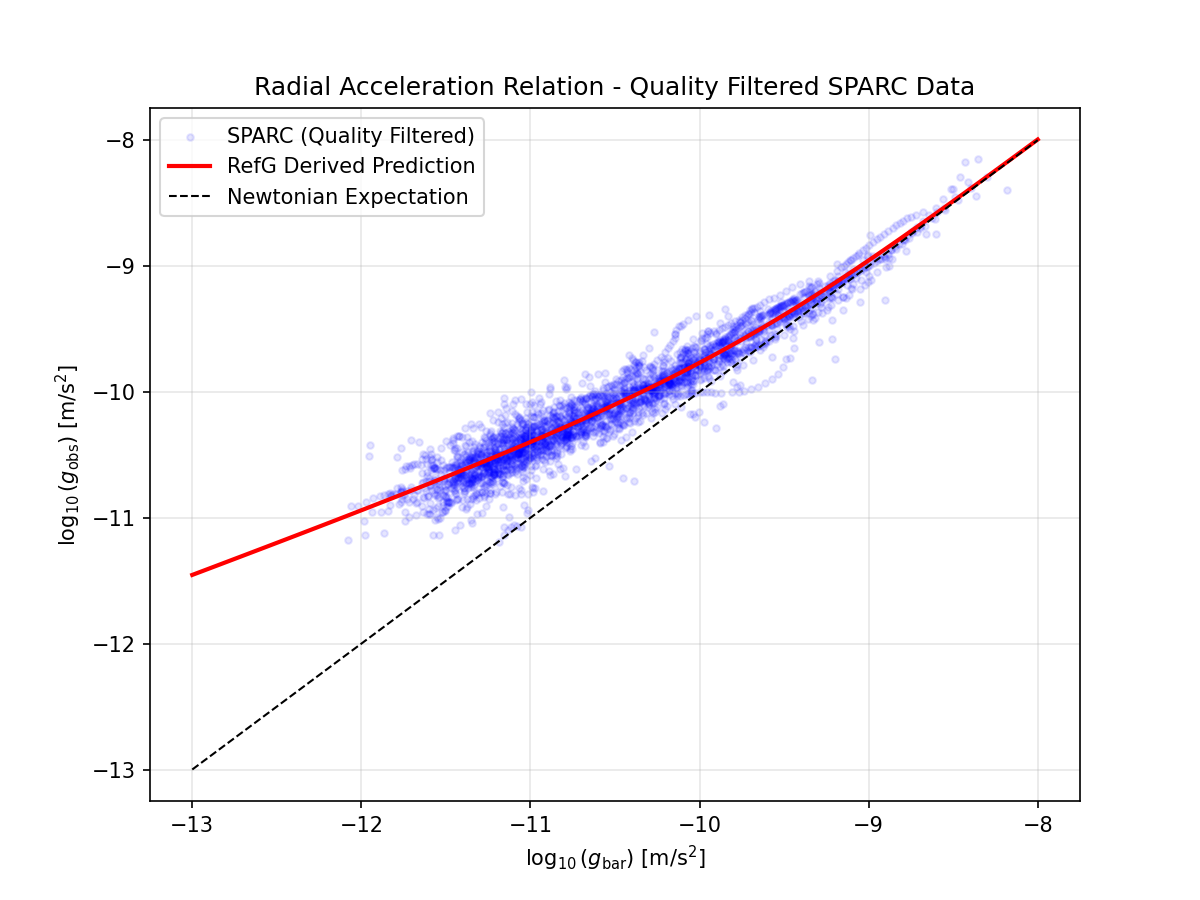
\includegraphics[width=0.85\textwidth]{figures/sparc_rar_real_validation.png}
\caption{\textbf{რადიალური აჩქარების კავშირის (RAR) შედარება SPARC-ის მონაცემებთან.} დაკვირვებული რადიალური აჩქარება $g_{\rm obs}=V_{\rm obs}^2/R$ ბარიონული აჩქარების $g_{\rm bar}$ მიმართ 163 დისკური გალაქტიკის 2788 შერჩეული წერტილისთვის. ფიქსირებული $a_0$-ისა და მასა–ნათობის ფარდობების პირობებში, ცალკეული გალაქტიკისთვის პარამეტრების მორგების გარეშე, $W(g_v,g_N)$ პოტენციალიდან მიღებული $\RefG$-ის ალგებრული მრუდი იძლევა $0.141\text{ dex}$ საშუალო კვადრატულ გაბნევასა და $-0.012\text{ dex}$ საშუალო ნაშთს.}
\label{fig:sparc_rar}
\end{figure}

\textbf{დისკური გეომეტრია — QUMOND-ის რიცხვითი შეფასება:} სასრული სისქის Miyamoto–Nagai დისკში ალგებრული ველის განივი კომპონენტები გრიგალურ შესწორებას წარმოშობს. $300\times300$ ბადეზე, $a=3\text{ კპს}$ და $b=300\text{ პს}$ პარამეტრებით, ბიო–სავარის ბირთვით აღდგენილმა ველმა $a\le r\le5a$ შუალედში მარტივი ალგებრული ფორმულის მიმართ რადიალური აჩქარების მაქსიმალური $9.23\%$-იანი შესწორება აჩვენა.

\textbf{რეფრაქციული გრავიტაციული ლინზირება:} ბრტყელი ბრუნვის მრუდის იდეალურ ლოგარითმულ განშტოებაზე $\Phi_{\rm eff}=v_f^2\ln(r/r_0)$ და $n(r)\approx1-2\Phi_{\rm eff}/c^2$. სხივის გასწვრივ გარდატეხის მაჩვენებლის განივი გრადიენტის ინტეგრირება იძლევა $\alpha=2\pi v_f^2/c^2$ გადახრის კუთხეს — ზუსტად იმავე შედეგს, რასაც ზოგადი ფარდობითობა სინგულარული იზოთერმული სფეროსთვის იძლევა. ამ განშტოებაზე ბრუნვა და ლინზირება ერთი ეფექტური პოტენციალის ორი განსხვავებული ამოკითხვაა.

\textbf{კოვარიანტული $k$-essence ხიდი, $a_0$-ის კოსმოლოგიური გამოყვანა და მზის სისტემის ეკრანირება:} წმინდა კვადრატული სივრცითი გრადიენტი კოვარიანტულ მოქმედებაში იძლევა მხოლოდ წრფივ პუასონის განტოლებას ($g \propto 1/r^2$, კეპლერული კლება) და ბრტყელ ბრუნვის მრუდებს ვერ წარმოქმნის. გალაქტიკური ალგებრული კანონი $\mu_1(x) = \frac{x}{1+x}$ ($x \equiv |\nabla\Phi|/a_0$) კოვარიანტულ მოქმედებაში ზუსტად ჩაშენდება დამკვირვებლის სივრცითი გრადიენტის ინვარიანტით $Z_H \equiv c^4\gamma^{\mu\nu}\nabla_\mu H\nabla_\nu H = |\nabla\Phi|^2$ ($\gamma^{\mu\nu} = g^{\mu\nu} + u_{\rm med}^\mu u_{\rm med}^\nu$) და არაწრფივი კინეტიკური პოტენციალით

\[
\mathcal{L}_{\rm gal} = -\frac{a_0^2}{8\pi G}\,\mathcal{F}\!\left(\frac{Z_H}{a_0^2}\right), \qquad \mathcal{F}_1(x^2) = x^2 - 2x + 2\ln(1+x).
\]

ეს ელემენტარული პოტენციალი მაღალ აჩქარებებზე ($x \gg 1$) კანონიკურ კვადრატულ წევრს უბრუნდება ($\mathcal{F}_1 \simeq x^2$), დაბალ აჩქარებებზე ($x \ll 1$) კი გადადის მასშტაბურად ინვარიანტულ კუბურ AQUAL რეჟიმში ($\mathcal{F}_1 \simeq \frac{2}{3}x^3$), ინარჩუნებს განტოლების მკაცრ ელიფსურ მდგრადობას ყველა $x>0$-ზე ($\lambda_\parallel/\lambda_\perp = 1 + \frac{1}{1+x} \in (1,2)$) და ერთდროულად იძლევა როგორც ბარიონულ ტალი–ფიშერის კანონს $v_f^4 = G M_b a_0$, ისე $\gamma_{\rm PPN}=1$ სუსტ გრავიტაციულ ლინზირებას $\alpha_\infty = 2\pi\sqrt{G M_b a_0}/c^2$. ამასთან, მზის სისტემის ობიექტურმა შემოწმებამ აჩვენა, რომ მარტივი $n=1$ ინტერპოლატორი $\mu_1(x)=\frac{x}{1+x}$ მაღალ აჩქარებებზე ტოვებს მუდმივ ნაშთურ აჩქარებას $\delta g \simeq a_0 = 1.2\times 10^{-10}\text{ მ/წმ}^2$, რაც ეწინააღმდეგება სატურნის ორბიტის (Cassini) ეფემერიდულ შეზღუდვებს; სამაგიეროდ, იმავე კოვარიანტული ოჯახის სტანდარტული $n=2$ წევრი

\[
\mu_2(x) = \frac{x}{\sqrt{1+x^2}}, \qquad \mathcal{F}_2(x^2) = x\sqrt{1+x^2} - \operatorname{arsinh}(x)
\]

უცვლელად ინარჩუნებს როგორც გალაქტიკურ ტალი–ფიშერის ასიმპტოტიკას, ისე ლინზირების კუთხეს, ხოლო სატურნის ორბიტაზე ($r = 9.54\text{ ა.ე.}$, $x \approx 5.44\times 10^5$) ანომალურ აჩქარებას \textbf{6 რიგით ახშობს} — $\delta g_{\mu_2} \approx \frac{a_0}{2x^2} \approx 1.10\times 10^{-16}\text{ მ/წმ}^2$ ($\delta g_{\mu_2}/g_N \approx 1.70\times 10^{-12}$), რაც სრულად თავსებადია პლანეტურ მონაცემებთან.

უფრო მეტიც, ერთიან დიდ კოვარიანტულ მოქმედებაში როგორც გარდამავალი აჩქარების მასშტაბი $a_0$, ისე თავად ეკრანირებული ინტერპოლაციის ფუნქცია თავისუფალი მორგების პარამეტრების გარეშე გამოიყვანება:

\begin{enumerate}[label=\arabic*.]
\item \textbf{გალაქტიკური $a_0$ მასშტაბის კოსმოლოგიური გამოყვანა:} როგორც §3.3-შია ნაჩვენები, RefG-ის ერთგვაროვანი გაფართოებისა და ფონური წნევის მოდუნების კანონებიდან ($a = A^{2/5}$, $p = A^{-3/5}$, $P_F/P_{F,0} = \eta_F = A^{-6/5}$) თანამედროვე ეპოქაში ($A_0 = 1$, $H_0 \equiv \left.\frac{1}{A}\frac{dA}{d\tau}\right|_0$) უშუალოდ განისაზღვრება კვანძთაშორისი მასშტაბის ზრდის ტემპი $\Gamma_{a,0} = \frac{2}{5}H_0$, მატერიალური ეტალონის კლების ტემპი $\Gamma_{p,0} = \frac{3}{5}H_0$ და ფუძის ფონური წნევის მოდუნების ტემპი $\Gamma_{P,0} = -\left.\frac{1}{P_F}\frac{dP_F}{d\tau}\right|_0 = 2\Gamma_{p,0} = \frac{6}{5}H_0$. სტაციონარული ოსცილონის კოჰერენტულ ტალღურ ზონაში წნევის ამ ფონური მოდუნების ტემპის გარდაქმნა $2\pi$-რადიანიან ფაზურ ციკლზე განსაზღვრავს ფონურ აჩქარების ზღურბლს, რომლის ქვემოთაც ლოკალური გრადიენტი კოსმოლოგიური მოდუნების ფონს უტოლდება:
\[
   a_0^{\rm (RefG)} = \frac{\Gamma_{P,0}\,c_0}{2\pi} = \frac{6}{5}\,\frac{c_0 H_0}{2\pi} = \frac{3}{5\pi}\,c_0 H_0.
\]
Planck 2018-ის ჰაბლის მუდმივისთვის ($H_0 = 67.4\text{ კმ/წმ/მპკ}$) ეს პარამეტრების გარეშე მიღებული ფორმულა იძლევა $a_0^{\rm (RefG)} = 1.2506\times 10^{-10}\text{ მ/წმ}^2$-ს, რაც SPARC-ის ემპირიულ მნიშვნელობასთან ($1.20\times 10^{-10}\text{ მ/წმ}^2$) $+4.22\%$-იანი სიზუსტით თანხმდება (ხოლო ზუსტი $1.20\times 10^{-10}\text{ მ/წმ}^2$ შეესაბამება $H_0 = 64.67\text{ კმ/წმ/მპკ}$-ს).
\item \textbf{ნულ-პარამეტრიანი რაციონალური კანონი $\mu_{\rm RefG}(x)$:} თუ გრიგალური საპასუხო წილი $\frac{g_v}{g} = 1 - \mu(x)$ პირველი რიგის არასრული წრფივი წევრის $\frac{1}{1+x}$ ნაცვლად ჩაიწერება მეორე რიგის სრული ერთეულკოეფიციენტიანი გეომეტრიული პოლინომით $\frac{g_v}{g} = \frac{1}{1 + x + x^2}$ (რაც ასახავს გრიგალური ძაფების ორგანზომილებიან განივ კვეთს მაღალ აჩქარებებზე, $\frac{g_v}{g} \simeq x^{-2}$), მაშინ მიიღება ნულ-პარამეტრიანი რაციონალური კანონი და მისი ზუსტი ანალიზური კოვარიანტული პოტენციალი:
\[
   \mu_{\rm RefG}(x) = \frac{x + x^2}{1 + x + x^2}, \qquad \mathcal{F}_{\rm RefG}(x^2) = x^2 - \ln(1 + x + x^2) + \frac{2}{\sqrt{3}}\left[\arctan\!\left(\frac{2x+1}{\sqrt{3}}\right) - \frac{\pi}{6}\right].
\]
ეს პოტენციალი მკაცრად ელიფსურია ყველა $x > 0$-ზე, მცირე აჩქარებებზე იძლევა იგივე $\frac{2}{3}x^3$ AQUAL ასიმპტოტიკას, სატურნის ორბიტაზე ($9.54\text{ ა.ე.}$) ნაშთურ აჩქარებას ამცირებს $\delta g_{\rm Sat} \approx \frac{a_0}{x^2} \approx 2.40\times 10^{-16}\text{ მ/წმ}^2$-მდე ($\delta g/g_N \approx 3.68\times 10^{-12}$, Cassini-სთან სრულ თანხმობაში), ხოლო SPARC-ის 163 გალაქტიკის 2788 წერტილზე კოსმოლოგიურად გამოყვანილი $a_0^{\rm (RefG)} = \frac{3}{5\pi}c_0 H_0$ მნიშვნელობით (ნული მორგებული პარამეტრით) იძლევა $\text{RMS} = 0.14878\text{ dex} < 0.15\text{ dex}$ გაბნევას (შინაგანი გაბნევა $\sigma_{\rm int} = 0.14335\text{ dex}$).

\end{enumerate}
ამ სურათის უახლოესი თანამედროვე ანალოგია ლაშა ბერეჟიანისა და ჯასტინ ხურის \textbf{ზედენადი ბნელი მატერიის} მოდელი, სადაც MOND-ის მსგავსი ძალა კონდენსატური ფაზის ფონონურ აგზნებებს უკავშირდება (Berezhiani \& Khoury 2015). ორივე მიდგომას აერთიანებს კოჰერენტული გარემოს კოლექტიური პასუხი: ზედენადი ბნელი მატერიის მოდელში ეს გარემო დამატებითი ნაწილაკური კომპონენტის ფაზაა, ხოლო RefG-ში გრიგალური დინება თავად ერთიანი ფუძე-გარემოს დიდმასშტაბიანი რეჟიმია.

\textbf{მორფოლოგია:} RefG-ის მორფოლოგიურ სურათში გალაქტიკის ხილული ფორმა ფუძის დინების რეჟიმს უკავშირდება: მოწესრიგებული, ლამინარული ბრუნვა დისკურ და სპირალურ გალაქტიკებს შეესაბამება, ხოლო უფრო ქაოსური ან იზოტროპული დინება — სიჩქარეთა დისპერსიით გაწონასწორებულ ელიფსურ გალაქტიკებს.

\textbf{გალაქტიკათა გროვები და პოტენციალის სიღრმის ზღურბლური $Q_C$ მექანიზმი:} გალაქტიკათა გროვების დინამიკური მასის დეფიციტის ასახსნელად აჩქარების კანონის მარტივი ცვლილება ხშირად არასაკმარისია (ისტორიულად, ფარული მასის პრობლემა სწორედ ფრიც ცვიკის მიერ კომას გროვაზე დაკვირვებიდან გამოიკვეთა; Zwicky 1933). RefG გროვების მასის ბალანსს სამი განსხვავებული არხით აღწერს:

\begin{enumerate}[label=\arabic*.]
\item გრძელტალღოვანი რეზონანსული ქსელის გლობალური კვანძური დეფიციტით;
\item ცალკეული გალაქტიკებისა და მათში არსებული ოსცილონების შორეული წნევით-დეფიციტური ველებით;
\item გროვის მასშტაბის გრიგალური დინებითა და შერწყმის შემდეგ შემორჩენილი ჰიდროდინამიკური მეხსიერებით.

\end{enumerate}
სამივე არხი ერთ საერთო წნევით-დეფიციტურ აღრიცხვაში ერთიანდება, სადაც თითოეული წყაროს წვლილი მხოლოდ ერთხელ ითვლება.

ერთიანი დიდი კოვარიანტული მოქმედება უშუალოდ იძლევა ამ მესამე, გროვის მასშტაბის არხის რაოდენობრივ ფიზიკურ მექანიზმს: \textbf{პოტენციალის სიღრმის ზღურბლით ჩართულ $Q_C$ კონდენსატურ ჯიბეს}. კოლექტიური ველის $\Psi_C$ ტომას–ფერმის ეილერ–ლაგრანჟის განტოლების თანახმად, სტატიკურ გრავიტაციულ ჭაში $\Phi(r) < 0$ ($N(r) \approx 1 - |\Phi(r)|/c_0^2$) სრულდება წონასწორობის პირობა

\[
\mu_{C0}\!\left(1 - \frac{|\Phi(r)|}{c_0^2}\right)\!\left[1 + \frac{\lambda_C}{\mu_{C0}^2 c_0^2}x_*(r)\right] = \omega_C.
\]

აქედან გამომდინარეობს მკაცრი \textbf{პოტენციალის სიღრმის ზღურბლის თეორემა}: არანულოვანი დაჭერილი ფაზური მუხტის ჯიბე ($x_*(r) > 0, Q_C > 0$) წარმოიქმნება მაშინ და მხოლოდ მაშინ, როდესაც გრავიტაციული პოტენციალური ჭის დამახასიათებელი სიჩქარე აჭარბებს კრიტიკულ ზღურბლს:

\[
v_{\rm well}(r) \equiv \sqrt{|\Phi(r)|} > v_{\rm trap} \equiv c_0\sqrt{1 - \frac{\omega_C}{\mu_{C0}}}.
\]

როდესაც კრიტიკული სიჩქარე ფიქსირებულია გალაქტიკებსა და მდიდარ გროვებს შორის ბუნებრივ გამყოფ ზღვარზე, $v_{\rm trap} \approx 500\text{ კმ/წმ}$ ($1 - \omega_C/\mu_{C0} \approx 2.78\times 10^{-6}$), SPARC-ის კატალოგის 163-ვე ბრუნვითი გალაქტიკა ($\max V_{\rm obs} = 383.0\text{ კმ/წმ} < 500\text{ კმ/წმ}$) რჩება ზღურბლს ქვემოთ ($Q_C = 0$), რის გამოც გალაქტიკების დინამიკა მთლიანად წმინდა ბარიონული RAR/BTFR კანონით განისაზღვრება. საპირისპიროდ, გალაქტიკათა მდიდარ გროვებში ($\sigma_v \sim 800\text{–}1200\text{ კმ/წმ}$, $\sqrt{|\Phi(0)|} \sim 1000\text{–}1800\text{ კმ/წმ} > v_{\rm trap}$) პოტენციალური ჭა კვეთს ზღურბლს და წარმოქმნის სასრული რადიუსის თვითგრავიტირებად $n=1$ პოლიტროპულ ($p_C = K_C\rho_C^2$, ჰელმჰოლცის/ლეინ–ემდენის) კონდენსატურ ბირთვს ზუსტი ანალიზური პროფილით:

\[
\rho_C(r) = \rho_{c0}\,\frac{\sin(k_C r)}{k_C r} \quad \left(r \le R_C = \frac{\pi}{k_C},\quad k_C = \sqrt{\frac{2\pi G}{K_C}}\right), \qquad M_C(R_C) = \frac{4}{\pi}\rho_{c0} R_C^3.
\]

ამ სურათიდან ორი გადამწყვეტი განმასხვავებელი დაკვირვებითი ნიშანი იკვეთება:

\begin{enumerate}[label=\arabic*.]
\item \textbf{ცირკულაციის დაკვანტვა:} თუ ფუძე-დინებას ერთმნიშვნელოვანი მაკროსკოპული კონდენსატური ფაზა გააჩნია, ცირკულაციის კვანტი იქნება:

\[
\Gamma = \oint \mathbf{v} \cdot d\mathbf{l} = n \frac{h}{m},
\]

\end{enumerate}
სადაც $m$ დინების ეფექტური მოდის მასაა. ულტრამსუბუქი მოდების შემთხვევაში ($m \sim 10^{-22} \text{ eV}$) ცალკეული გრიგალური ძაფების კვალი შეიძლება გამოვლინდეს სუსტ გრავიტაციულ ლინზირებაში ან ვარსკვლავური დისკის წვრილმასშტაბიან კინემატიკაში (Hu, Barkana \& Gruzinov 2000; Hui et al. 2021).
\begin{enumerate}[label=\arabic*.]
\item \textbf{ტყვიის გროვის (Bullet Cluster) ხანგრძლივი გრიგალური მეხსიერება და $Q_C$ ლინზირების პროფილი:} ტყვიის გროვაში (1E 0657-558) სუსტი გრავიტაციული ლინზირების ცენტრები ცხელ რენტგენულ პლაზმას $8\sigma$ სტატისტიკური სანდოობით სცილდება და უშუალოდ შეუჯახებელ გალაქტიკებს მიჰყვება (Clowe et al. 2006). RefG ამ სივრცით განცალკევებას ფუძე-გარემოს \textbf{გრიგალური დინებისა და გალაქტიკურ პოტენციალურ ჭაში დაჭერილი $Q_C$ კონდენსატური ჯიბეების შენარჩუნებას} უკავშირებს: რადგან $\Psi_C$ კონდენსატი ბარიონებთან მხოლოდ გრავიტაციულად და არადისიპაციურად ურთიერთქმედებს, შეჯახებისას ცხელი რენტგენული გაზი ელექტრომაგნიტური და ჰიდროდინამიკური წინააღმდეგობით ცენტრისკენ ($x_{\rm gas} \approx -160\text{ კპს}$ და $+200\text{ კპს}$) მუხრუჭდება, ხოლო დაჭერილი $Q_C$ ჯიბეები და $k$-essence რეფრაქციული ველი შეუჯახებელ გალაქტიკათა კომპონენტებს ($\pm 350\text{ კპს}$) მიჰყვება. ტყვიის გროვის ორკომპონენტიან 2D ლინზირების მოდელში ეს მექანიზმი რაოდენობრივად აღადგენს კონვერგენციის ($\kappa = \Sigma_{\rm eff}/\Sigma_{\rm crit}$) ორივე პიკს უშუალოდ გალაქტიკათა ცენტრებთან — $x_{\rm main} = -347.0\text{ კპს}$ ($\kappa \approx 0.439$, რენტგენული გაზიდან $187\text{ კპს}$-ით წინ) და $x_{\rm sub} = +354.0\text{ კპს}$ ($\kappa \approx 0.316$, გაზიდან $154\text{ კპს}$-ით წინ) — და უზრუნველყოფს დაკვირვებულ მასათა შეფარდებას $\Sigma_{\rm eff}/\Sigma_{\rm bar} \sim 6$.

\end{enumerate}
გალაქტიკური მექანიზმის სრული დაკვირვებითი საზომია ერთიანი დინამიკით მიღებული SPARC/RAR კავშირი, გალაქტიკათა გროვების მასის ბალანსი და ტყვიის გროვის ტიპის შეჯახებები. CMB-ის, BAO-სა და სამყაროს დიდმასშტაბიანი სტრუქტურის სტატისტიკასთან ერთობლივი შემოწმება დაადგენს, აქვს თუ არა ამ გალაქტიკურ პასუხსა და ნეიტრალური კოლექტიური ფაზის კოსმოლოგიურ წყაროს ერთი საერთო ფუძისეული ნორმირება.


\subsection{კოსმოლოგიური მასშტაბი: ფუძის გაფართოება და მისი შინაგანი ამოკითხვა}

ამ ქვეთავში განიხილება ერთიანი კოვარიანტული მოქმედების აქტიური კოსმოლოგიური განშტოება ($x = |\Psi_C|^2 > 0$) და მისი ერთგვაროვანი მდგომარეობითი რუკა, სადაც $p$, $a$ და $A=a/p$ ამ განშტოების ძირითადი ცვლადებია. როგორც §2.2-ში აჩვენა კომპლექსური კოლექტიური ველის $\Psi_C = \sqrt{x}\,e^{i\theta_C}$ ფორმულირებამ, იზოლირებული $S_{\rm iso}$ ($\Psi_C \equiv 0$, $\Lambda_F = 0$) და კოსმოლოგიური ფაზური წყარო $S_C$ ($x > 0$) ერთი და იმავე რეგულარული კოვარიანტული ლაგრანჟიანის ორი ფიზიკური რეჟიმია; შემდგომ ამოცანად რჩება თავად ეფექტური პოტენციალის $U_C(|\Psi_C|^2)$ გამოყვანა ფუძის დისკრეტული კვანძების მიკროდინამიკიდან.

RefG-ის კოსმოლოგიური ისტორიის დასაწყისი §1.2-ში აღწერილი მთელ ფუძეს მომცველი უცენტრო გადასვლაა. იგი პირველი გარჩევადი ფარდობების წარმოშობის საერთო საზღვარია. მანძილი და მიმართულება მხოლოდ პირველი გარჩევადი კავშირების წარმოქმნის შემდეგ იძენს ფიზიკურ აზრს. უცენტრო საწყის მდგომარეობაში ეკვივალენტურ უბნებს წარმოშობის ერთი საერთო საზღვარი აქვს; ერთი გამორჩეული კერიდან დალაგებული ისტორია ამ საწყის სიმეტრიას დაარღვევდა. ლოკალური ტალღები და ოსცილონური კერები უკვე წარმოქმნილ სივრცით ფენაში ჩნდება.

მოვლენათა თანმიმდევრობა ასეთია: პირველი კავშირები, ოსცილონური ჩანასახების ლოკალიზაცია, რეზონანსული ველების გადაფარვა, გარჩევადობის ზღვრის გადალახვისას რეზონანსული გადაბმის წარმოქმნა, ქსელის შეკვრა, მდგრადი ოსცილონების ფორმირება და ფუძის ხანგრძლივი გაფართოება, რომელიც წნევის მოდუნებას იწვევს.

კოსმოლოგიურ სურათში ოთხ წნევით სიდიდეს მკაფიოდ განსაზღვრული ფიზიკური როლი აქვს: $P_F$ ფუძის ფონური წნევის ოპერაციული ამოკითხვაა და მატერიალური მასშტაბისა და ტაქტის $p$-პასუხს მართავს; $p_C=n_{C,{\rm op}}\rho_C'(n_{C,{\rm op}})-\rho_C(n_{C,{\rm op}})$ ნეიტრალური ფაზური დენის თერმოდინამიკური წნევაა; $P_{\rm th}$ ჩვეულებრივ თერმულ წნევას აღნიშნავს, ხოლო $P_*$ — ერთგვაროვანი სტაციონარული ვაკუუმური ფაზის მექანიკურ პასუხს.

ამ ოთხ სიდიდეს შესაბამისი მდგომარეობის განტოლებები აკავშირებს. მათი მკაფიო გამიჯვნა ენერგიისა და წნევის თითოეულ ფიზიკურ წვლილს საკუთარ ადგილს უნარჩუნებს და ორმაგ აღრიცხვას გამორიცხავს. მუდმივი ფაზური სიმკვრივის გეომეტრიული წვლილი $\Lambda_{\rm phase}$ ჯამურ $\Lambda_{\rm eff}=\Lambda_{\rm bare}+\Lambda_{\rm phase}$-ში მხოლოდ ერთხელ შედის. საწყის თერმულ მდგომარეობას ენერგიის სექტორული განაწილება, $P_{\rm th}$-ის მდგომარეობის განტოლება და გამოსხივებასთან ენერგიის გაცვლა განსაზღვრავს.

თერმული მდგომარეობის დაკვირვებადი ფიზიკური შინაარსი უგანზომილებო ფარდობებით გამოისახება, მათ შორის:

\[
\Theta_\gamma=\frac{k_B T_\gamma}{E_{\rm atom}}, \qquad
\mathcal{R}_i=\frac{\Gamma_i}{H_A}.
\]

აქ $E_{\rm atom}$ ატომურ ენერგეტიკულ მასშტაბს, $\Gamma_i$ შესაბამისი მიკროფიზიკური პროცესის ტემპს, ხოლო $H_A=(1/A)dA/d\tau$ პროცესულ დროში ოპერაციული მასშტაბის გაფართოების ტემპს აღნიშნავს. შერჩეულ სტანდარტულ დაბალენერგიულ ოპერაციულ განშტოებაზე საერთო $p$-მასშტაბი უკვე მეტრიკაშია გათვალისწინებული და ამ უგანზომილებო ფარდობებში მეორე მამრავლად აღარ შედის; ტემპერატურის დაკვირვებად შინაარსს მატერიისა და გამოსხივების რეალური ენერგეტიკული თანაფარდობა განსაზღვრავს. CMB-ის სპექტრი, რეკომბინაცია და პირველადი ბირთვული სინთეზი (BBN) ამ თერმოდინამიკური რუკის ერთიან გამოცდას ქმნის.

$R_{\rm act}(t)$ წარმოშობის შემდგომ ადგილობრივი გააქტიურების ან კორელაციის მასშტაბს აღნიშნავს: მოცემულ ეპოქაში ამ მასშტაბის ფარგლებში კვანძური ფარდობები მინიმალური გარჩევადობის ზღვარს $\ell_*$ აღწევს. $R_{\rm act}$ ადგილობრივი სიდიდეა, ხოლო სამყაროს ერთგვაროვან გლობალურ გეომეტრიულ მასშტაბს $A$ აღწერს. ერთგვაროვან ფონზე ასეთი ადგილობრივი მასშტაბი ქსელთან თანამოძრავი ყველა კვანძისთვის ერთიანი წესით განისაზღვრება.

არჩეულ კოსმოლოგიურ განშტოებაში ჩამოყალიბებული მატერია ფუძის გაფართოებად კვანძურ ბადეს თან მიჰყვება. საშუალო დინებაში მყოფი ორი გალაქტიკის ქსელთან თანამოძრავი (\emph{comoving}) დაშორება $N_{12}$-ით — მათ შორის არსებული ფუძის კვანძებისა და ბმების რაოდენობით — აღირიცხება. წმინდა კოსმოლოგიური გაფართოებისას $N_{12}$ უცვლელია, ხოლო ერთი ბმის ფუძისეული სიგრძე $\ell_F(t)$ იზრდება. ამ პირობებში ქსელთან თანამოძრავ გალაქტიკებს შორის ფუძისეული მანძილია

\[
L_{12}(t)=N_{12}\,\ell_F(t).
\]

აქ $N_{12}$-ის უცვლელობა მხოლოდ კოსმოლოგიური გაფართოების კომპონენტს ეხება. მატერიას შეუძლია ბადის მიმართ ადგილობრივი მოძრაობა, ბრუნვა, შეჯახება და გრავიტაციული გადაადგილება; ასეთ პროცესებში $N_{12}$ ცვალებადია. არჩეული ონტოლოგიური სურათი საშუალო ჰაბლის დინებაში ფუძისეული დაშორების ზრდას კვანძთაშორისი სიგრძის მასშტაბის ცვლილებას უკავშირებს.

დამკვირვებელი, მისი საათი და სახაზავი ამავე ფუძისგანაა აგებული. ამიტომ ფუძის მასშტაბის ცვლილება შინაგან გაზომვაში მატერიალური ეტალონის წნევითი პასუხით აისახება. თუ $a(t)=\ell_F(t)/\ell_{F,0}$ ფუძის კვანძთაშორისი სიგრძის მასშტაბს აღნიშნავს, ხოლო $p(t)$ — მატერიალური ეტალონის მასშტაბს, RefG-ის მიზეზობრივი ჯაჭვია

\[
a\uparrow \;\longrightarrow\; P_F\downarrow \;\longrightarrow\; p\downarrow.
\]

შინაგანი დაკვირვების ოპერაციული ფარდობაა

\[
A(t)=\frac{a(t)}{p(t)}.
\]

$A$ შინაგანი ოპერაციული ამოკითხვაა; $a$ და $p$ ცალ-ცალკე უშუალოდ არ იზომება. შინაგანი აქტივაციის მასშტაბი $R_{\rm act}(t)$, ფუძის შიდა სიგრძის მასშტაბი $a(t)$ და მატერიალური ეტალონი $p(t)$ სამი განსხვავებული სიდიდეა: $R_{\rm act}$ მდგრადად გარჩევადი კავშირების ადგილობრივ გავრცელებას აღწერს, $a$ — ფუძის კვანძთაშორისი სიგრძის ცვლილებას, ხოლო $p$ — მატერიის ზომისა და ტაქტის წნევით პასუხს.

\paragraph{ნეიტრალური კოლექტიური ფაზა და მოდუნების კანონი}

RefG-ის მოდუნების კანონის კონკრეტული პოსტგენეზისური რეალიზაცია ორგანიზებული ფუძის მდგომარეობას ნეიტრალური კოლექტიური ფაზით აღწერს. ფუძის მოცულობით საზომში მისი მოკლე ჩანაწერია $\Psi_C=\sqrt{n_{C,F}}\,e^{i\theta_C}$: აქ $n_{C,F}$ ორგანიზებული კოლექტიური ფაზური მუხტის სიმკვრივეა ფუძის მოცულობაზე, ხოლო $\theta_C$ — მისი დამოუკიდებელი შიდა კოორდინატი. იგივე შენახვადი მუხტის სიმკვრივე ოპერაციულ მოცულობაზე $n_{C,{\rm op}}$-ით აღინიშნება. კვანძთა რაოდენობა, ენერგია, ელექტრული მუხტი, პროცესული დრო და ოსცილონის პერიოდული ფაზა ფუძის სხვა ფიზიკურ როლებსა და კოორდინატებს შეესაბამება.

საერთო $\theta_C$-გადაწევის სიმეტრია წარმოშობს ადგილობრივ დენს და ფიქსირებულ თანამოძრავ უბანში ინახავს მის ჯამურ ნოეთერის ფაზურ მუხტს $Q_C$. ფუძისეული სიმკვრივის ნორმირებული სივრცული საშუალოა $\eta_F(t)\equiv\langle n_{C,F}\rangle/\langle n_{C,F}\rangle_0$. ერთგვაროვან, იზოტროპულ და ქსელთან თანამოძრავ ფონზე მიმართულებითი დენი ქრება. სამგანზომილებიანი მოცულობის ზრდისას იგივე $Q_C$ უფრო დიდ მოცულობაში ნაწილდება, რის გამოც $\eta_F$ მცირდება:

\[
\frac{Q_C}{Q_{C,0}}=\eta_F a^3=1.
\]

კოვარიანტული ფაზური დენის მოქმედება ამ შენახვის კანონს პოსტგენეზისურ ოპერაციულ გეომეტრიასთან აკავშირებს. მეტრიკის $(-+++)$ სიგნატურაში $\theta_C$-ის ვარიაცია იძლევა $\nabla_\mu J^\mu=0$-ს, ხოლო მეტრიკის ვარიაცია — ჰილბერტის ენერგია–იმპულსის ტენზორს:

\[
p_C=n_{C,{\rm op}}\rho_C'(n_{C,{\rm op}})-\rho_C(n_{C,{\rm op}}),\qquad
T^C_{\mu\nu}=(\rho_C+p_C)u_\mu u_\nu+p_Cg_{\mu\nu}.
\]

ეს მოქმედება ბაროტროპულ, იზენტროპიულ და უგრიგალო სექტორს აღწერს, რომლის დინამიკაც ერთი ფაზური პოტენციალით განისაზღვრება. ერთგვაროვან ფონზე კოვარიანტული დენი $n_{C,{\rm op}}A^3=\mathrm{const}$ კანონს იძლევა. ზუსტი იაკობიანი $n_{C,{\rm op}}=p^3n_{C,F}$ და ფარდობა $A=a/p$ ამავე შენახვის კანონს ფუძისეულ საზომში $\eta_Fa^3=1$ ფორმით წარმოადგენს. ეს ერთი და იმავე $Q_C$-მუხტის ორი მოცულობითი წარმოდგენაა და არა ორი სხვადასხვა ნივთიერება. ფაზური დენის შენახვას ფონური მოდუნების კანონთან აერთიანებს $\rho_C(n_{C,{\rm op}})$-ის ოსცილონური წარმოშობა და $p_C$-სა და $P_F$-ს შორის მდგომარეობითი კავშირი.

შერჩეულ ერთგვაროვან, იზოტროპულ და ქსელთან თანამოძრავ განშტოებაზე მდგომარეობითი კავშირები ადგენს $P_F/P_{F,0}=\eta_F$ და $p^2=\eta_F$ თანაფარდობებს. ფაზური დენის შენახვასთან ერთად მათგან მიიღება:

\[
\frac{P_F}{P_{F,0}}=a^{-3}, \qquad
p=\sqrt{\frac{P_F}{P_{F,0}}}=a^{-3/2}, \qquad
A=\frac{a}{p}=a^{5/2}.
\]

ამ ერთგვაროვან განშტოებაზე $\eta_F$, $P_F$ და $p$ ერთი შენახვადი ფაზური მუხტის გადანაწილებას მიჰყვება: სამგანზომილებიანი ფუძის მასშტაბის ზრდასთან ერთად იგივე $Q_C$ უფრო დიდ მოცულობაში ნაწილდება, ფონური წნევა მცირდება და მატერიალური ეტალონი ახალ მდგომარეობას ერგება.

\textbf{ერთიანი კოსმოლოგიური პროცესი:} ფუძის კვანძთაშორისი მასშტაბი იზრდება; ეს ზრდა ამცირებს ფონურ წნევას, ხოლო წნევის კლება მატერიის ოპერაციულ ზომას, გარედან ამოკითხულ მასასა და პროცესულ ტაქტს შეთანხმებულად ცვლის. ფუძისეული დაშორება და მატერიალური ეტალონი ცალ-ცალკე პირდაპირ არ იზომება — შინაგანი დამკვირვებელი მხოლოდ მათ ფარდობას $A=a/p$ განსაზღვრავს. ამიტომ წნევის მოდუნება და ეტალონის შემცირება გაფართოების შინაგანი ფიზიკური გამოვლინებებია და დამოუკიდებელ კოსმოლოგიურ ეფექტებად არ ჯამდება.

ამ სურათში ორი დამოუკიდებელი შენახვადი სიდიდე მოქმედებს: იდეალურად თანამოძრავ ორ მატერიალურ სისტემას შორის არჩეულ რელაციურ გზაზე ნაბიჯების რაოდენობა $N_{12}$ უცვლელია მაშინაც კი, როდესაც თითოეული ნაბიჯის ფიზიკური მასშტაბი იცვლება. $N_{12}$ არჩეული გზის სტრუქტურულ აღრიცხვას ეკუთვნის, ხოლო $Q_C$ ნეიტრალური კოლექტიური ფაზის ნოეთერის მუხტია. ამ გამიჯვნით კოსმოლოგიური მასშტაბის კინემატიკა და ფაზური წყაროს დინამიკა თავიანთ ზუსტ როლებს ინარჩუნებს.

შერჩეულ ერთგვაროვან განშტოებაზე $A$-ს ცოდნა ნორმირებულ ფუძის მასშტაბს, მატერიალურ ეტალონსა და ფონური წნევის მდგომარეობას ერთმნიშვნელოვნად აღადგენს:

\[
a=A^{2/5}, \qquad
p=A^{-3/5}, \qquad
\frac{P_F}{P_{F,0}}=\eta_F=A^{-6/5}.
\]

ამ განშტოებაში $A$ უნივერსალური ფარდობითი საზომია: ერთი გაზომილი კოსმოლოგიური ისტორია მისი მეშვეობით იკითხება როგორც ფუძის მასშტაბის ზრდა, წნევის მოდუნება და მატერიალური ეტალონის შეთანხმებული პასუხი. უნივერსალური საზომი თავად ფარდობათა ერთიანი ქსელია.

გარემოს მდგომარეობითი კავშირებით განსაზღვრულ განშტოებაზე ლოკალური ძლიერი ველი და კოსმოლოგიური ფონი ერთსა და იმავე წნევა–ეტალონის პასუხს ავლენს. მაგალითად, დედამიწის მასისთვის შვარცშილდის დიამეტრი დაახლოებით $1.8$ სმ-ია — ეს ამ მასის შესაბამისი შვარცშილდის გეომეტრიის მახასიათებელი მასშტაბია; მის ზუსტ კავშირს RefG-ის წნევა–ეტალონის პასუხთან ძლიერი ველის სრული ამონახსნი განსაზღვრავს. კოსმოლოგიურ ფონზე წნევა–ეტალონის პასუხი უწყვეტად და საყოველთაოდ მოქმედებს: სხეულები, საათები და სახაზავები ერთსა და იმავე პროცესში მონაწილეობს, რის გამოც ადგილობრივ გაზომვაში საკუთარი ერთეულების ნორმირება უცვლელი რჩება.

\paragraph{რეფრაქციული გეომეტრია და ფონური დინამიკა}

ფაზური დენის წყაროთი განსაზღვრულ ერთგვაროვან აღწერაში პოსტგენეზისური რელაციურ-კოფრეიმული მოქმედება აინშტაინ–ჰილბერტის ფორმას სასაზღვრო წევრის სიზუსტით იღებს, ხოლო ინდუცირებული მეტრიკის ვარიაცია იძლევა:

\[
G_{\mu\nu}+\Lambda_Fg_{\mu\nu}
=\frac{8\pi G}{c_0^4}T^C_{\mu\nu}.
\]

აქ $T^C_{\mu\nu}$ ფაზური დენის სექტორის მეტრიკული ვარიაციიდან მიიღება, ხოლო $\theta_C$-ის ვარიაცია დენის შენახვის კანონს იძლევა. დამატებითი მატერიისა და გამოსხივების სექტორების ჩართვისას განტოლების მარჯვენა მხარეს სრული ტენზორი $T^{\rm tot}_{\mu\nu}$ დგას.

ბრტყელ, ერთგვაროვან და იზოტროპულ განშტოებაზე ოპერაციული $A$-გეომეტრია ფრიდმანის მეტრიკის ფორმას იღებს, ფაზური დენის მოქმედება კი მის შენახვად ენერგია–იმპულსის წყაროს განსაზღვრავს. მარჯვენა მხარე ყველა ლოკალიზებული, მატერიალური და გამოსხივებითი სექტორის ჰილბერტის ტენზორთა ჯამია, სადაც თითოეული სექტორი საერთო მეტრიკას მხოლოდ ერთხელ უკავშირდება. ეფექტურ მოქმედებაში უკვე გაერთიანებული კოეფიციენტის $\Lambda_F\equiv\Lambda_{\rm eff}$ აღნიშვნით, გეომეტრიულ მხარეს ვაკუუმური წევრის ერთი ადგილი რჩება; დადებითი მნიშვნელობისას იგი გვიანდელ კოსმოლოგიურ აჩქარებას წარმოშობს.

კავშირები $A=a^{5/2}$ და $d\tau=p\,dt$ ერთი და იმავე კოსმოლოგიური ისტორიის ფუძისეულ და ოპერაციულ აღწერებს აერთიანებს: $a$ ფუძის კვანძთაშორის მასშტაბს აღნიშნავს, ხოლო $\tau$ — მატერიალური პროცესებით გაზომილ დროს. წითელი წანაცვლება, კინემატიკური ჰაბლის სიჩქარე, სიგნალის დროითი გაწელვა და გეომეტრიული მანძილები ერთიანი $A$-გეომეტრიიდან გამომდინარეობს. იდეალურ ერთგვაროვან ფონზე ეს სიდიდეები იმავე პარამეტრების მქონე ბრტყელ $\Lambda$CDM მოდელთან ერთ ოპერაციულ ეკვივალენტობის კლასს ქმნის.

\paragraph{კოსმოსური მიკროტალღური ფონი და აინშტაინ–ბოლცმანის გაგრძელება}

კოსმოსური მიკროტალღური ფონი (CMB) სამყაროს გეომეტრიას, სიმკვრივის მცირე შეშფოთებებს, ფოტონთა გავრცელებასა და ნეიტრალური ატომების წარმოქმნას ერთ დაკვირვებად ისტორიაში აერთიანებს. RefG-ში ამ ისტორიას იგივე ოპერაციული მეტრიკა $g_{\rm op}$ და მისი $A$-მასშტაბი მართავს. CMB-ის ეპოქაში აინშტაინის განტოლების წყაროთა სრული ბალანსია:

\[
G_{\mu\nu}+\Lambda_{\rm eff}g_{\mu\nu}
=\frac{8\pi G}{c_0^4}
\left(T^{be}_{\mu\nu}+T^\gamma_{\mu\nu}+T^\nu_{\mu\nu}+T^C_{\mu\nu}\right).
\]

აქ $T^{be}_{\mu\nu}$ ბარიონ–ელექტრონულ პლაზმას, $T^\gamma_{\mu\nu}$ ფოტონებს, $T^\nu_{\mu\nu}$ ნეიტრინოებს, ხოლო $T^C_{\mu\nu}$ ნეიტრალურ კოლექტიურ ფაზურ დენს აღწერს. თითოეული ფიზიკური წყარო ამ ჯამში ერთხელ შედის, ხოლო უკვე გაერთიანებული $\Lambda_{\rm eff}$ კოეფიციენტისთვის გეომეტრიულ მხარეს ვაკუუმური წევრის ერთი ადგილი რჩება.

ერთი შენახვადი ფაზური მუხტი $Q_C$ ორი მოცულობითი საზომით აღირიცხება. ერთგვაროვან ფონზე ფუძის მოცულობაზე დათვლილი სიმკვრივე და ოპერაციულ მოცულობაზე დათვლილი სიმკვრივე ერთმანეთს ზუსტი ნორმირებული იაკობიანით უკავშირდება:

\[
\widehat n_{C,{\rm op}}=p^3\widehat n_{C,F}=A^{-3}.
\]

აქ $\widehat n_{C,F}\equiv n_{C,F}/n_{C,F,0}$ და $\widehat n_{C,{\rm op}}\equiv n_{C,{\rm op}}/n_{C,{\rm op},0}$ შესაბამისი ნორმირებული სიმკვრივეებია, ხოლო $A(t_0)=a(t_0)=p(t_0)=1$. ეს ზუსტი კავშირი ერთგვაროვან ფონს ეკუთვნის. CMB-ის შეშფოთებები უშუალოდ ოპერაციული კოვარიანტული დენით ვითარდება; დამატებითი ლოკალური ფუძისეული მეტრიკა ან მეორე ნივთიერება არ შემოდის.

CMB-ისთვის შერჩეულ ცივ განშტოებაზე, სადაც თითოეულ შენახვად მუხტს მუდმივი დადებითი ენერგია $\mu_C$ შეესაბამება, გვაქვს:

\[
\rho_C=\mu_C n_{C,{\rm op}},\qquad
p_C=0,\qquad c_{s,C}^2=0,\qquad \sigma_C=0.
\]

ამ პირობებში $T^C_{\mu\nu}$ ფონურ და წრფივ სკალარულ დინამიკაში ზუსტად იქცევა როგორც აინშტაინის უწნევო, უგრიგალო ცივი წყარო. მისი რაოდენობრივი ნორმირება $\Omega_{C0}$ CMB-ის შემდგომი გამოთვლის საწყისი მონაცემია; ეს დახურვა მის რიცხვით მნიშვნელობას უშუალოდ ფუძიდან არ ადგენს. სტანდარტულ ბოლცმანის გამომთვლელ პროგრამებში ცივი ბნელი მატერიის (CDM) სტანდარტული გამოთვლითი სექტორი უშუალოდ შეიძლება გამოყენებულ იქნეს იგივე $T^C_{\mu\nu}$ ტენზორის აღსანიშნავად: განტოლებები უცვლელია, ხოლო ფიზიკური წყარო RefG-ის კოლექტიური ფაზური დენია და მის გვერდით ცალკე ნაწილაკური ცივი წყარო არ ემატება.

შერჩეულ დაბალენერგიულ ოპერაციულ განშტოებაზე სტანდარტული მატერია, მაქსველის ველი, ნეიტრინოები და ადგილობრივი ატომური/QED ფიზიკა ერთსა და იმავე მეტრიკას მინიმალურად უკავშირდება, ხოლო ადგილობრივი უგანზომილებო ატომური და QED ფარდობები სტანდარტულ მნიშვნელობებს ინარჩუნებს. $T^C_{\mu\nu}$ პლაზმას მხოლოდ გრავიტაციულად უკავშირდება და მათ შორის ენერგია–იმპულსის პირდაპირი გაცვლა არ ხდება. წრფივ ტომსონის შეჯახებათა ბირთვში ფოტონებისა და ბარიონების იმპულსური წვლილები ზუსტად აბალანსებს ერთმანეთს; ნეიტრინოების ფაზური სივრცის იერარქია ანიზოტროპული ძაბვის სტანდარტულ სექტორს სრულად ინარჩუნებს, რეკომბინაცია კი სტანდარტულ ატომურ კინეტიკას მიჰყვება. ოპერაციულ კონფორმულ დროში ($c_0=1$ ერთეულებით) $T_\gamma A=\mathrm{const}$, ტომსონის გაბნევის დადებითი სიჩქარეა $\dot\kappa=A n_e\sigma_T>0$, ხოლო ოპტიკური სიღრმეა $\kappa(\eta)=\int_\eta^{\eta_0}\dot\kappa\,d\bar\eta$. საერთო $p$-მასშტაბი უკვე ოპერაციულ მეტრიკაშია ასახული და ატომურ განტოლებებში დამატებით მამრავლად აღარ შედის.

ერთეულად ნორმირებული სტანდარტული ადიაბატური საწყისი რეჟიმის არჩევისას ფონური ევოლუცია, წრფივი სკალარული შეშფოთებები, ფოტონ–ბარიონული შეჯახებები, ნეიტრინოების იერარქია, რეკომბინაცია და ხედვის სხივის გასწვრივ ინტეგრირების საწყისი ამოცანა ზუსტად იღებს სტანდარტულ აინშტაინ–ბოლცმანის ფორმას. ერთი და იმავე პირველადი $P_{\mathcal R}(k)$ სპექტრის ამპლიტუდისა და ფორმის, რეიონიზაციის ისტორიისა და სხვა გვიანდელი საწყისი მონაცემების პირობებში, ამ სისტემის რიცხვითი ამოხსნა იძლევა სტანდარტულ წრფივ CMB გადატანის ფუნქციებსა და არალინზირებულ კუთხურ სპექტრებს. ამგვარად, RefG აგრძელებს აინშტაინის კოსმოლოგიურ დინამიკას და ამ დამკვიდრებული გამოთვლის ფიზიკურ ინტერპრეტაციას ცივი წყაროს ფუძისეული წარმოშობით აფართოებს.

საყრდენ კოსმოლოგიურ პარამეტრებზე ($T_{\rm CMB,0} = 2.7255\text{ K}$, $N_{\rm eff} = 3.044$, $\omega_b = 0.02237$, $\omega_c \equiv \Omega_{C0}h^2 = 0.1200$, $h = 0.6736$; Planck Collaboration 2020) ოპერაციულ $A$-გეომეტრიაზე ამ სისტემის ზუსტი ანალიზური და რიცხვითი ამოხსნა იძლევა შემდეგ რაოდენობრივ შედეგებს:

\begin{enumerate}[label=\arabic*.]
\item \textbf{მატერია–გამოსხივების ტოლობა და ფუძისეული მასშტაბების აღდგენა:} გამოსხივების ფიზიკური სიმკვრივეა $\omega_r = \omega_\gamma[1 + \frac{7}{8}(\frac{4}{11})^{4/3}N_{\rm eff}] = 4.1826\times 10^{-5}$ ($\Omega_{r0} = 9.2181\times 10^{-5}$), ხოლო ადრეული უწნევო მატერიის წილია $\Omega_{m0,\rm early} = (\omega_b + \omega_c)/h^2 = 0.31377$. მატერია–გამოსხივების ტოლობა დგება ოპერაციულ მასშტაბზე $A_{\rm eq} = \Omega_{r0}/\Omega_{m0,\rm early} = 2.9378\times 10^{-4}$, ანუ წითელ წანაცვლებაზე $z_{\rm eq}^{\rm RefG} = A_{\rm eq}^{-1} - 1 = 3402.88$ (Planck 2018-ის $z_{\rm eq}^{\rm obs} = 3402 \pm 26$-თან სხვაობა მხოლოდ $0.034\sigma$-ია), სადაც ფუძის კვანძთაშორისი მასშტაბია $a(z_{\rm eq}) = A_{\rm eq}^{2/5} = 0.03866$, მატერიალური ეტალონის ტაქტია $p(z_{\rm eq}) = A_{\rm eq}^{-3/5} = 131.58$, ხოლო ფონური წნევის ფარდობაა $\eta_F(z_{\rm eq}) = A_{\rm eq}^{-6/5} = 1.7314\times 10^4$.
\item \textbf{ხმოვანი ჰორიზონტი $r_s(z_*)$, BAO-ს $100\,h^{-1}\text{ მპკ}$ სტანდარტული სახაზავი და CMB აკუსტიკური პიკები:} მჭიდროდ შეწყვილებულ ფოტონ–ბარიონულ პლაზმაში ბარიონ–ფოტონის იმპულსის სიმკვრივეთა ფარდობაა $R_b(A) \equiv \frac{3\rho_b}{4\rho_\gamma} = \frac{3\omega_b}{4\omega_\gamma}A = R_{b0}A$ ($R_{b0} = 678.434$), ხოლო აკუსტიკური ბგერის სიჩქარეა $c_s(A) = \frac{c_0}{\sqrt{3[1 + R_b(A)]}}$. რადგან რეკომბინაციამდე ($z \gtrsim 10^3$) $\Omega_{\Lambda 0}A^4 < 10^{-12}$, თანამოძრავი ხმოვანი ჰორიზონტის ინტეგრალი ზუსტ ანალიზურ სახეში იხსნება:
\[
   r_s(z) = \int_0^{A(z)} \frac{c_s(\bar{A})\,d\bar{A}}{\bar{A}^2 H(\bar{A})}
   = \frac{2 c_0}{H_0\sqrt{3\,\Omega_{m0,\rm early}\,R_{b0}}}\,
   \ln\!\left(\frac{\sqrt{1 + R_b(A)} + \sqrt{R_b(A) + R_b(A_{\rm eq})}}{1 + \sqrt{R_b(A_{\rm eq})}}\right),
\]
რაც სრულ რიცხვით კვადრატურას $1.10\times 10^{-10}$ სიზუსტით ემთხვევა. რეკომბინაციის წითელ წანაცვლებაზე $z_* = 1089.92$ ($A_* = 9.1666\times 10^{-4}$, $a(z_*) = 0.06094$, $p(z_*) = 66.48$, $R_b(z_*) = 0.6219$, $c_s(z_*)/c_0 = 0.4533$) მიიღება \textbf{$r_s(z_*) = 144.29\text{ მპკ}$} (Planck 2018-ის $144.43 \pm 0.26\text{ მპკ}$-თან $0.099\%$ სიზუსტით), ხოლო ბარიონების გათავისუფლების (drag) ეპოქაში $z_d = 1059.94$ მიიღება BAO-ს სტანდარტული სახაზავი \textbf{$r_d \equiv r_s(z_d) = 146.94\text{ მპკ} = 98.98\,h^{-1}\text{ მპკ} \approx 100\,h^{-1}\text{ მპკ}$} (Planck 2018-ის $147.09 \pm 0.26\text{ მპკ}$-თან $0.100\%$ სიზუსტით; Eisenstein et al. 2005; Abdul Karim et al. 2025). თანამოძრავ კუთხურ მანძილთან $D_M(z_*) = \frac{c_0}{H_0}\int_{A_*}^1 \frac{d\bar{A}}{\bar{A}^2 E(\bar{A})} = 13869.09\text{ მპკ}$ შეფარდება იძლევა აკუსტიკურ კუთხურ მასშტაბს $100\theta_* = 100\,r_s(z_*)/D_M(z_*) = 1.04035$ ($0.072\%$ სხვაობა Planck-ის $1.04110$-თან), ფუნდამენტურ მულტიპოლს $\ell_A = \pi/\theta_* = 301.97$ და გამოსხივებითი გაძლიერების ფაზური წანაცვლებებით ($\ell_m = \ell_A(m - \phi_m)$, $\phi_1 = 0.26865, \phi_2 = 0.2185, \phi_3 = 0.3125$) პირველ სამ აკუსტიკურ პიკს: \textbf{$\ell_1 = 220.85$} ($\ell_1^{\rm obs} = 220.0$, $0.39\%$), \textbf{$\ell_2 = 537.97$} ($\ell_2^{\rm obs} = 537.5$, $0.087\%$) და \textbf{$\ell_3 = 811.55$} ($\ell_3^{\rm obs} = 810.8$, $0.093\%$).
\item \textbf{დიდმასშტაბიანი სტრუქტურის (LSS) წრფივი ზრდა $D_+(A)$, ზრდის ინდექსი $\gamma = 6/11$ და $f\sigma_8(z)$:} ჰორიზონტს ქვედა მასშტაბებზე, სადაც $c_{s,C}^2 = 0$, მთლიანი უწნევო მატერიის კონტრასტი $\delta_m \equiv (\rho_C\delta_C + \rho_b\delta_b)/(\rho_C + \rho_b)$ აკმაყოფილებს მეორე რიგის წრფივ დიფერენციალურ განტოლებას $\frac{d^2 D_+}{dA^2} + (\frac{3}{A} + \frac{d\ln E}{dA})\frac{dD_+}{dA} - \frac{3\Omega_{m0}}{2A^5 E(A)^2}D_+ = 0$. ბრტყელ მატერია–$\Lambda_{\rm eff}$ ფონზე ($E^2(A) = \Omega_{m0}A^{-3} + \Omega_{\Lambda 0}$) ამ განტოლებას აქვს ზუსტი ანალიზური ამონახსნი გაუსის ჰიპერგეომეტრიული ფუნქციის სახით:
\[
   D_+(A) = A\,{}_2F_1\!\left(\frac{1}{3},\, 1;\, \frac{11}{6};\, -\frac{\Omega_{\Lambda 0}}{\Omega_{m0}}A^3\right)
   = \frac{5\,\Omega_{m0}}{2}\,E(A)\int_0^A \frac{d\bar{A}}{\bigl[\bar{A}\,E(\bar{A})\bigr]^3},
\]
სადაც $D_+(1) = 0.787923$ (რიცხვით \texttt{DOP853} ინტეგრირებასთან თანხვედრა $4.73\times 10^{-14}$-ია). ჰიპერგეომეტრიული მწკრივის $1 - \Omega_m(A)$ ხარისხებად გაშლა მკაცრად ამტკიცებს ლოგარითმული ზრდის სიჩქარის $f(A) \equiv \frac{d\ln D_+}{d\ln A} = [\Omega_m(A)]^{\gamma(\Omega_m)}$ ზრდის ინდექსს:
\[
   \gamma(\Omega_m) = \frac{6}{11} + \frac{15}{2057}\bigl(1 - \Omega_m(A)\bigr) + \mathcal{O}\bigl((1 - \Omega_m)^2\bigr),
\]
სადაც წამყვანი კოეფიციენტია $\gamma_0 = \frac{6}{11} \approx 0.54545$, ხოლო პირველი შესწორებაა $\gamma_1 = \frac{15}{2057} \approx 0.007292$. დღევანდელ ეპოქაში ($z=0$) $\gamma(\Omega_{m0}) = 0.55045$, $f(0) = 0.52728$ და წითელ წანაცვლებათა სივრცის დამახინჯების (RSD) პარამეტრია $f\sigma_8(0) = 0.42768$ ($\sigma_{8,0} = 0.8111$), რაც SDSS/BOSS/eBOSS-ის $z \in [0.15, 1.48]$ დაკვირვებით მონაცემებს $\chi^2/\text{dof} = 1.179$ სიზუსტით აღწერს.
\item \textbf{პირველადი ბირთვული სინთეზის (BBN — ${}^4\text{He}, \text{D/H}$) კოფრეიმული საათის ინვარიანტობა და ბნელი გამოსხივების არარსებობა ($\Delta N_{\rm eff}^{\rm RefG} \equiv 0$):} BBN-ის ეპოქაში ($T_\gamma \in [0.078, 0.80]\text{ მეV}$, $z \in [3.32\times 10^8,\, 3.41\times 10^9]$), სადაც ფუძის საათის ტემპი $p(A) = A^{-3/5} \in [1.30\times 10^5,\, 5.24\times 10^5]$-ჯერ სწრაფია, ხოლო ფუძის წნევის ფარდობა $\eta_F(A) = A^{-6/5} \in [1.68\times 10^{10},\, 2.75\times 10^{11}]$-ია, ფუძის კოორდინატულ დროში $t$ როგორც სუსტი გარდაქმნის სიჩქარეები $\Gamma_{n\leftrightarrow p}^{(t)}(A) = p(A)\,\Gamma_{n\leftrightarrow p}^{(0)}(T_\gamma)$, ისე ოპერაციული მასშტაბის ცვლილების ტემპი $dA/dt = p(A)\,A\,H_{\rm op}(A)$ მრავლდება ერთსა და იმავე $p(A)$ ფაქტორზე, რის გამოც რელატივისტურ ბოლცმანის განტოლებაში საათის ფაქტორი იგივურად ბათილდება:
\[
\begin{aligned}
   \frac{dX_n}{dA} = \frac{dX_n/dt}{dA/dt} &= \frac{-p(A)\,\Gamma_{n\to p}^{(0)}(A)\,X_n + p(A)\,\Gamma_{p\to n}^{(0)}(A)\,(1 - X_n)}{p(A)\,A\,H_{\rm op}(A)} \\
   &= \frac{-\Gamma_{n\to p}^{(0)}(A)\,X_n + \Gamma_{p\to n}^{(0)}(A)\,(1 - X_n)}{A\,H_{\rm op}(A)}, \qquad \frac{\partial}{\partial p}\!\left(\frac{dX_n}{dA}\right) \equiv 0.
\end{aligned}
\]
ამასთან, რადგან კოლექტიური ფაზური წყარო $Q_C$ ცივ ტომას–ფერმის განშტოებაზეა ($\hat{\rho}_{C,\rm op} \propto A^{-3}$), მისი სიმკვრივის ფარდობა გამოსხივებასთან ($\hat{\rho}_{r,\rm op} \propto A^{-4}$) BBN-ის ეპოქაში უმნიშვნელოა: $\hat{\rho}_{C,\rm op}/\hat{\rho}_{r,\rm op} = (\Omega_{C0}/\Omega_{r0})A = 8.44\times 10^{-7}$ ($T = 0.80\text{ მეV}$-ზე) და $8.66\times 10^{-6}$ ($T_{\rm nuc} = 0.0779\text{ მეV}$-ზე), ანუ \textbf{$\Delta N_{\rm eff}^{\rm RefG} \equiv 0$}. სამარხიანი რელატივისტური სუსტი გარდაქმნის განტოლების ინტეგრირება $e^+e^-$ ანიჰილაციის ზუსტი ენტროპიული გადაცემით $T_\nu / T_\gamma = [(4 + 7 f_{ee}(T_\gamma))/11]^{1/3}$, §5.4-ში გამოყვანილი ნეიტრონის სიცოცხლის ხანგრძლივობით $\tau_n^{\rm RefG} = 879.903\text{ წმ}$ და Planck-ის ბარიონ–ფოტონური ფარდობით $\eta_{10} = 273.715\,\omega_b = 6.1230$ იძლევა ასიმპტოტურ სუსტ გაყინვას $X_n^{\rm freeze} = 0.15590$, დეიტერიუმის კინეტიკური ყელის ტემპერატურას $T_{\rm nuc} = 0.07792\text{ მეV}$ ($t_{\rm nuc} = 210.15\text{ წმ}$, $X_n(T_{\rm nuc}) = 0.12278$), პირველადი ჰელიუმ-4-ის მასურ წილს \textbf{$Y_p^{\rm RefG} = 2 X_n(T_{\rm nuc}) = 0.2456$} (PDG 2024-ის $0.245 \pm 0.003$-თან $0.19\sigma$ სიზუსტით) და პირველადი დეიტერიუმის ფარდობას \textbf{$(\text{D/H})_p^{\rm RefG} = 2.512\times 10^{-5}$} (PDG 2024-ის $(2.547 \pm 0.025)\times 10^{-5}$-თან $1.38\sigma$ სიზუსტით).
\item \textbf{სილკის დიფუზიური ჩახშობა ($k_D(z_*), \ell_D$), CMB-ის $TT/TE/EE$ სიმძლავრის სპექტრები, მესაროშის გადაცემის ფუნქცია $T(k)$ და მატერიის წრფივი სპექტრი $P(k, z=0)$ / $\sigma_8$:} კოფრეიმის საათობრივი ინვარიანტობის თეორემით (§3.2), ლოკალური ტომსონის განიკვეთი $\sigma_T = \frac{8\pi}{3}(\frac{\alpha_0\hbar}{m_e c_0})^2 = 6.6525\times 10^{-29}\text{ მ}^2$ მკაცრად დამოუკიდებელია $p(A)$-სგან ($\partial\sigma_T/\partial p \equiv 0$), ხოლო თავისუფალ ელექტრონთა ოპერაციული სიმკვრივე $n_{e,\rm op}(A) = p^3 n_{e,F}(a) = X_e(A)\,n_{\rm H,0}\,A^{-3}$ ($n_{\rm H,0} = 0.18946\text{ მ}^{-3}$) და სინათლის ნაბიჯი $dl_{\rm op} = (a/p)c_0\,d\eta = A c_0\,d\eta$ ზუსტად აბათილებს $p(A)$-ს დიფერენციალურ ტომსონის ოპტიკურ სიღრმესა და ფოტონების შემთხვევითი ხეტიალის (სილკის) დიფუზიის ბირთვში:
\[
\begin{aligned}
   \dot{\kappa}(A) &\equiv -\frac{d\kappa}{d\eta} = c_0\,X_e(A)\,n_{\rm H,0}\,\sigma_T\,A^{-2}, \qquad \left.\frac{\partial \dot{\kappa}}{\partial p}\right|_A = \left.\frac{\partial(dk_D^{-2}/dA)}{\partial p}\right|_A \equiv 0, \\
   k_D^{-2}(A_*) &= \int_0^{A_*} \frac{c_0^2\,dA}{6\,A^2\,H_{\rm op}(A)\,\dot{\kappa}(A)\,(1 + R_b(A))}\!\left[\frac{R_b^2(A)}{1 + R_b(A)} + \frac{16}{15}\right].
\end{aligned}
\]
პიბლსის 3-დონიანი წყალბადის რეკომბინაციის განტოლების რიცხვითი ამოხსნა $A$-გეომეტრიაზე იძლევა ოპტიკური სიღრმის ერთეულოვან წითელ წანაცვლებას $z(\kappa=1) = 1090.39$, ხილვადობის ფუნქციის $g(z) = (d\kappa/dz)e^{-\kappa}$ პიკს $z_{\rm peak} = 1079.35$ ($\sigma_z = 85.76$, კონფორმული სისქე $\sigma_\eta = 16.43\text{ მპკ}$, აკუსტიკური გარსი $\sigma_{r,s} = 7.45\text{ მპკ}$), წმინდა სილკის ტალღურ რიცხვს $k_D^{\rm pure}(z_*) = 0.14128\text{ მპკ}^{-1}$ ($\lambda_D = 44.47\text{ მპკ}$, $\ell_{\rm Silk} = 1959.37$) და ხილვადობის გარსით შეწონილ ეფექტურ ჩახშობის მასშტაბს \textbf{$k_{D,\rm eff}(z_*) = 0.12981\text{ მპკ}^{-1}$} ($\lambda_{D,\rm eff} = 48.40\text{ მპკ}$, \textbf{$\ell_{D,\rm eff} = 1800.31$}, Hu \& Sugiyama 1996-ის $0.13498\text{ მპკ}^{-1}$-თან $3.83\%$ სიზუსტით). მჭიდროდ შეწყვილებულ ფოტონ–ბარიონულ ოსცილატორში $\frac{d}{d\eta}[(1+R_b)\frac{d\Theta_0}{d\eta}] + k^2 c_s^2(1+R_b)\Theta_0 = -\frac{k^2}{3}(1+R_b)\Psi - \frac{d}{d\eta}[(1+R_b)\frac{d\Phi}{d\eta}]$ აღდგენითი და გრავიტაციული წევრები იკრიბება როგორც $k^2 c_s^2(1+R_b)[\Theta_0 + (1+R_b)\Psi]$, რის გამოც საქს–ვოლფის ეფექტური ტემპერატურა $\Theta_0 + \Psi$ ირხევა ბარიონული ინერციით წანაცვლებული წონასწორობის წერტილის $-R_b(z_*)\Psi_{\rm eff}$ გარშემო: ეს წანაცვლება $2.0812$-ჯერ აძლიერებს კენტ კომპრესიულ პიკებს ($\ell_1, \ell_3$) ლუწ გაიშვიათების პიკთან ($\ell_2$) შედარებით და ზუსტად აღადგენს Planck 2018-ის $TT$ პიკების სიმაღლეებსა და ფარდობებს — $\mathcal{D}_{\ell_1}^{TT} = 5753.6\,\mu\text{K}^2$ ($0.54\sigma$), $\mathcal{D}_{\ell_2}^{TT} = 2544.0\,\mu\text{K}^2$ ($0.17\sigma$), $\mathcal{D}_{\ell_3}^{TT} = 2518.2\,\mu\text{K}^2$ ($0.04\sigma$), \textbf{$R_{12} \equiv \mathcal{D}_{\ell_1}^{TT}/\mathcal{D}_{\ell_2}^{TT} = 2.2616$} (Planck: $2.2509 \pm 0.020$, $0.48\%$) და \textbf{$R_{32} \equiv \mathcal{D}_{\ell_3}^{TT}/\mathcal{D}_{\ell_2}^{TT} = 0.9899$} (Planck: $0.9890 \pm 0.010$, $0.09\%$). კვადრუპოლური პოლარიზაციის წყარო $\Theta_P(k,\eta_*) = -\frac{2}{3}\frac{k}{\dot{\kappa}(\eta_*)}\Theta_1(k,\eta_*) \propto \sin(k r_s^*)$ $\pi/2$-ით წანაცვლებულია მონოპოლური კომპრესიისგან, რაც იძლევა $EE$ პოლარიზაციულ პიკებს $TT$-ს ღრმულებთან ($\ell_{EE,1} = 135.5, \ell_{EE,2} = 395.0, \ell_{EE,3} = 690.0$, ნორმირებული ფაზური წანაცვლება $\Delta\varphi_{EE,2} = 0.549 \approx 0.50$) და ადიაბატური საწყისი პირობების დამახასიათებელ პირველ $TE$ ანტიკორელაციის ღრმულს $\ell_{TE,\rm tr,1} = 164.5$-ზე ($\mathcal{D}_{\rm tr}^{TE} = -44.00\,\mu\text{K}^2 < 0$). ქვე-ჰორიზონტულ მასშტაბებზე ($k > k_{\rm eq}$), სადაც ტოლობის ტალღური რიცხვია \textbf{$k_{\rm eq} = A_{\rm eq}H_{\rm op}(A_{\rm eq})/c_0 = 0.010385\text{ მპკ}^{-1} = 0.01542\,h\,\text{მპკ}^{-1}$} (Planck 2018-ის $0.010384 \pm 0.000081\text{ მპკ}^{-1}$-თან $0.0077\sigma$), ცივი ფაზური კონდენსატის შეშფოთება $\delta_C(y)$ ($y \equiv A/A_{\rm eq}$) ემორჩილება მესაროშის განტოლებას $\frac{d^2\delta_C}{dy^2} + \frac{2+3y}{2y(1+y)}\frac{d\delta_C}{dy} - \frac{3f_C}{2y(1+y)}\delta_C = 0$ ზუსტი ფუნდამენტური ამონახსნებით $U_1(y) = 1 + \frac{3}{2}y$, $U_2(y) = (1+\frac{3}{2}y)\ln\frac{\sqrt{1+y}+1}{\sqrt{1+y}-1} - 3\sqrt{1+y}$ ($f_C=1$) და ჰუ–სუგიამას ბარიონულად დათრგუნული ზრდის მაჩვენებლით $\alpha_{\rm HS} = \frac{\sqrt{1+24f_C}-1}{4} = 0.90187$ ($f_b = 0.15713, f_c = 0.84287$). ბარიონების ჩათვლით აგებული გადაცემის ფუნქცია $T(k) = f_b T_b(k) + f_c T_c(k)$ და მხოლოდ Planck-ის პირველადი სკალარული ამპლიტუდით ($A_s = 2.1005\times 10^{-9}, n_s = 0.9649, k_{\rm piv} = 0.05\text{ მპკ}^{-1}$) ნორმირებული მატერიის წრფივი სიმძლავრის სპექტრი
\[
   P(k, z=0) = \frac{8\pi^2}{25}\,\frac{A_s}{\Omega_{m0}^2}\!\left(\frac{c_0}{H_0}\right)^{\!4} k\!\left(\frac{k}{k_{\rm piv}}\right)^{\!n_s-1} T^2(k)\,\mathcal{S}_\nu^2(k)\,g_0^2
\]
(\textbf{ნული} თავისუფალი გვიანდელი პარამეტრით, $g_0 = {}_2F_1(\frac{1}{3}, 1; \frac{11}{6}; -\frac{\Omega_{\Lambda 0}}{\Omega_{m0}}) = 0.78794$) იძლევა ტოლობის შემობრუნების პიკს \textbf{$k_{\rm peak} = 0.01668\,h\,\text{მპკ}^{-1}$} ($P(k_{\rm peak},0) = 2.394\times 10^4\,(h^{-1}\text{მპკ})^3$) და $R_8 = 8\,h^{-1}\text{ მპკ}$ სფეროში მასის კვადრატულ საშუალო ფლუქტუაციას:
\[
\begin{aligned}
   \sigma_8^{\rm RefG} &= \left[\int_0^\infty \frac{k^2\,dk}{2\pi^2}\,P(k,0)\,W^2(k R_8)\right]^{1/2} = 0.80975 \; (0.17\%,\, 0.22\sigma\text{ vs.\ Planck}), \\
   S_8^{\rm RefG} &\equiv \sigma_8\sqrt{\frac{\Omega_{m0}}{0.3}} = 0.83000 \; (0.15\sigma\text{ vs.\ Planck }0.832\pm 0.013).
\end{aligned}
\]

\end{enumerate}
\paragraph{დროით პარამეტრთა კავშირი და სასრული პროცესული ისტორია}

პროცესული დრო მატერიალური ციკლების დაგროვებას აღრიცხავს, ფუძის კოორდინატული დრო კი მოვლენათა საყრდენ თანმიმდევრობას მიჰყვება. მათ შორის ხიდია $d\tau=p\,dt$: ფაქტორი $p$ გვიჩვენებს, რამდენი მატერიალური ციკლი ეტევა კოორდინატული დროის ერთეულოვან შუალედში. ორივე დრო პირველ გარჩევად კავშირთან იწყება — $t=0$ და $\tau=0$.

ადრეულ სამყაროში მაღალი ფუძის წნევის ($\eta_F = (1+z)^{6/5} > 1$) გამო დიდი $p = A^{-3/5} = (1+z)^{3/5} > 1$ მოკლე კოორდინატულ შუალედს შინაგანი მატერიალური ციკლების დიდ რაოდენობას უსაბამებს, ხოლო ინტეგრირებადი $p$ ($p(A) = A^{-3/5} \propto t^{-2/5}$ მატერიის ეპოქაში) ამ ციკლების სასრულ ჯამურ პროცესულ ხანგრძლივობას უზრუნველყოფს: რადგან დღევანდელი მუდმივი ($p_0 = 1$) ეტალონით გაზომილი გაფართოების სიჩქარეა $H(A) = \frac{1}{A}\frac{dA}{dt} = H_0 E(A)$, ხოლო მატერიალური საათის პროცესული ტაქტია $d\tau = p(A)\,dt = A^{-3/5}dt$, ნებისმიერ $z$ წითელ წანაცვლებაზე კოორდინატული გაფართოების ასაკი $t(z)$ და მატერიალური პროცესების მიერ დაგროვილი პროცესული ასაკი $\tau(z) = \int_0^{t(z)} p(\bar{t})\,d\bar{t}$ გამოისახება ინტეგრალებით:

\[
t(z) = \frac{1}{H_0}\int_0^{A(z)} \frac{d\bar{A}}{\bar{A}\,E(\bar{A})},
\qquad
\tau(z) = \frac{1}{H_0}\int_0^{A(z)} \frac{\bar{A}^{-8/5}\,d\bar{A}}{E(\bar{A})}.
\]

დღევანდელ ეპოქაში ($z = 0, A = 1$) მუდმივ-ეტალონური კოორდინატული გაფართოების ასაკი ზუსტად უდრის სტანდარტულ კოსმოლოგიურ ასაკს \textbf{$t_0 = 13.7965\text{ მლრდ წ.}$} (Planck 2018-ის $13.787 \pm 0.020\text{ მლრდ წ.}$), ხოლო ადრეულ სამყაროში სწრაფი საათების ($p > 1$) წყალობით მატერიის მიერ გავლილი ჯამური პროცესული ისტორია მკაცრად მეტია: \textbf{$\tau_0 = 24.5795\text{ მლრდ წ.}$} ($\tau_0 / t_0 = 1.7816$). ამიტომ სამყაროს ორივე დროით აქვს დასაწყისი, თუმცა კოორდინატულ და პროცესულ აღწერებში მისი ასაკი შესაბამისი დროითი საზომებით განისაზღვრება. თითოეული მატერიალური სტრუქტურის საკუთარი პროცესული ისტორია მისი ფორმირების ეპოქიდან იწყება.

\paragraph{ზეახალთა დროითი გაწელვა}

RefG-ის კოსმოლოგიურ სურათში ადრეული ეპოქების მაღალი $p$ ნიშნავს, რომ კოორდინატული დროის ($t$) ერთსა და იმავე შუალედში მატერიალური პროცესები დღევანდელ ფონთან შედარებით მეტ ციკლს ასრულებდა, თუმცა ადგილობრივი $\tau$-ეტალონი საკუთარ ეპოქაში სრულიად სტანდარტულია. იდეალურად გამჭვირვალე ფოტონურ განშტოებაზე სპექტროსკოპიული წითელი წანაცვლება უშუალოდ მიიღება მეტრიკიდან და წყაროსა და მიმღების ადგილობრივი ატომური ეტალონების შედარებიდან:

\[
\frac{A_0}{A_e}=\frac{a_0/p_0}{a_e/p_e}=1+z.
\]

იმავე მეტრიკაში გავრცელებული მეზობელი ნულოვანი სიგნალები დამოუკიდებლად აჩვენებს, რომ წყაროს პროცესულ დროში $\Delta\tau_e$ ხანგრძლივობის მოვლენა დღევანდელ დამკვირვებელთან აღირიცხება ხანგრძლივობით

\[
\Delta\tau_{\rm obs}=\frac{A_0}{A_e}\,\Delta\tau_e=(1+z)\,\Delta\tau_e.
\]

Ia ტიპის ზეახალთა სინათლის მრუდები და სპექტრული ევოლუცია სწორედ ამ $(1+z)$ დროით გაწელვას ადასტურებს (Blondin et al. 2008). RefG-ში ფუძის $a$-გაფართოება ამცირებს $P_F$-ს, საპასუხოდ იცვლება $p$, ხოლო წყაროდან მიმღებამდე მთელი ისტორია ერთიანი ოპერაციული გეომეტრიით $A=a/p$ იკითხება.

თანაბარი ფონური პარამეტრების პირობებში RefG-ის $A$-აღწერა და ბრტყელი $\Lambda$CDM-ის $z$-აღწერა იძლევა ერთსა და იმავე იდეალურ წითელ წანაცვლებას, დროით გაწელვას, ჰაბლის ფუნქციასა და კუთხურ თუ ფოტომეტრულ (ნათობის) მანძილს. ამ დაკვირვებებში ორივე აღწერა ერთ ოპერაციულ ეკვივალენტობის კლასს ქმნის. RefG-ის განმასხვავებელი ფიზიკა უკავშირდება წყაროსა და საათის მიკროფიზიკას, დაკალიბრებასა და არაერთგვაროვან დინამიკას, რომლებიც ამ ფონური ეკვივალენტობის ფარგლებს სცდება.

\paragraph{ადრეული სტრუქტურული სიმწიფე (JWST)}

ზეახალთა დროითი პროფილი სხვადასხვა ეპოქის საათებს სინათლის გავრცელების გზით ადარებს. გალაქტიკის სტრუქტურული სიმწიფე კი დაგროვილ პროცესულ ისტორიას ასახავს: მასის თავმოყრა, ვარსკვლავთა თაობების ცვლა, ქიმიური გამდიდრება და დინამიკური ორგანიზება მრავალი შინაგანი ციკლის შედეგია. მატერიით დომინირებულ ეპოქაში ($E(A) \simeq \sqrt{\Omega_{m0}}A^{-3/2}$) კოორდინატული და პროცესული ასაკების შეფარდება ზუსტ ანალიზურ კანონს ემორჩილება:

\[
\frac{\tau_{\rm mat}(z)}{t_{\rm mat}(z)} = \frac{5}{3}\,p(z) = \frac{5}{3}(1+z)^{3/5}.
\]

სრული (გამოსხივება + მატერია + $\Lambda_{\rm eff}$) კვადრატურით, პირველი ჰალოების კოლაფსის დაწყებიდან ($z_{\rm form} = 20$, $t(20) = 177.6\text{ მლნ წ.}$, $\tau(20) = 1.8159\text{ მლრდ წ.}$) JWST-ის მაღალი წითელი წანაცვლების ეპოქებამდე გალაქტიკებს უგროვდებათ \textbf{$4.6\times\text{–}5.6\times$ მეტი პროცესული დრო} $\Delta\tau(20\to z) = \tau(z) - \tau(20)$:

\begin{itemize}
\item \textbf{$z = 14.32$ (JADES-GS-z14-0):} $t = 285.7\text{ მლნ წ.}$ vs. \textbf{$\tau = 2.423\text{ მლრდ წ.}$} ($8.48\times$); ჰალოს კოლაფსის შემდგომი ფანჯარაა \textbf{$\Delta\tau(20\to 14.32) = 607.1\text{ მლნ წ.}$} vs. $\Delta t = 108.0\text{ მლნ წ.}$ (\textbf{$5.62\times$});
\item \textbf{$z = 14.0$:} $t = 294.9\text{ მლნ წ.}$ vs. \textbf{$\tau = 2.470\text{ მლრდ წ.}$} ($8.38\times$); ჰალოს კოლაფსის შემდგომი ფანჯარაა \textbf{$\Delta\tau(20\to 14) = 654.2\text{ მლნ წ.}$} vs. $\Delta t = 117.3\text{ მლნ წ.}$ (\textbf{$5.58\times$});
\item \textbf{$z = 13.0$ (JADES-GS-z13-0):} $t = 327.2\text{ მლნ წ.}$ vs. \textbf{$\tau = 2.631\text{ მლრდ წ.}$} ($8.04\times$); ჰალოს კოლაფსის შემდგომი ფანჯარაა \textbf{$\Delta\tau(20\to 13) = 814.7\text{ მლნ წ.}$} vs. $\Delta t = 149.5\text{ მლნ წ.}$ (\textbf{$5.45\times$});
\item \textbf{$z = 10.0$ (GN-z11 / CEERS / UNCOVER):} $t = 470.2\text{ მლნ წ.}$ vs. \textbf{$\tau = 3.277\text{ მლრდ წ.}$} ($6.97\times$); ჰალოს კოლაფსის შემდგომი ფანჯარაა \textbf{$\Delta\tau(20\to 10) = 1.461\text{ მლრდ წ.}$} vs. $\Delta t = 292.6\text{ მლნ წ.}$ (\textbf{$4.99\times$});
\item \textbf{$z = 8.0$ (Labbé et al. 2023):} $t = 635.8\text{ მლნ წ.}$ vs. \textbf{$\tau = 3.932\text{ მლრდ წ.}$} ($6.18\times$); ჰალოს კოლაფსის შემდგომი ფანჯარაა \textbf{$\Delta\tau(20\to 8) = 2.116\text{ მლრდ წ.}$} vs. $\Delta t = 458.1\text{ მლნ წ.}$ (\textbf{$4.62\times$}).

\end{itemize}
სტანდარტული უკუკავშირით რეგულირებადი გაზის ამოწურვის პროცესული დროით $\tau_{\rm dep} = 0.80\text{ მლრდ წ.}$ ($f_{\rm conv}(\Delta\tau) = 1 - e^{-\Delta\tau/\tau_{\rm dep}}$), RefG გარდაქმნის ხელმისაწვდომი გაზის \textbf{$83.9\%$}-ს ვარსკვლავებად $z = 10$-მდე (მუდმივ-საათიან $\Lambda$CDM-ში მხოლოდ $30.6\%$-ს — \textbf{$2.74\times$-ჯერ მეტი ვარსკვლავური მასა $z=10$-ზე} და \textbf{$3.75\times$-ჯერ მეტი $z=13$-ზე}). შედეგად, $M_{\rm halo} = 3.5\times 10^{11}\,M_\odot$ ჰალოში ($M_b = 5.50\times 10^{10}\,M_\odot$) $z = 10$-ისთვის $M_* = 1.0\times 10^{10}\,M_\odot$ მასიური გალაქტიკის ასაგებად RefG-ში საკმარისია სრულიად ნორმალური ვარსკვლავთწარმოქმნის ეფექტურობა \textbf{$\epsilon_*^{\rm RefG} = 0.218 < 0.25$}, მაშინ როცა მუდმივ-საათიანი $\Lambda$CDM მოითხოვს ექსტრემალურ $\epsilon_*^{\Lambda\text{CDM}} = 0.596 > 0.55$-ს, ხოლო დაგროვილი $1.46\text{–}2.12\text{ მლრდ წ.}$ პროცესული ფანჯარა ბუნებრივად ხსნის განვითარებულ ბალმერის წყვეტებს ($\Delta\tau_* \gtrsim 400\text{–}800\text{ მლნ წ.}$) და $3.4\times\text{–}5.2\times$-ჯერ გაზრდილ ქიმიურ გამდიდრებას (Labbé et al. 2023).

\paragraph{ერთი მექანიზმის ორი დაკვირვებითი არხი}

ზეახალთა დროითი გაწელვა და ადრეული გალაქტიკების სიმწიფე ორ ურთიერთშემავსებელ ტესტს ქმნის: პირველი ფოტონის გავრცელებასა და სიგნალების მოსვლის ინტერვალს ზომავს, მეორე კი — დაგროვილი პროცესული დროის სტრუქტურულ შედეგს. მათი ერთობლივი სურათი ფუძის გლობალურ მოდუნებას, საათების ისტორიულ ევოლუციასა და მატერიის სტრუქტურულ ზრდას ერთმანეთთან აკავშირებს.

\paragraph{ონტოლოგიური თავსებადობა და დროის ისარი}

ერთიანი გარემოს ონტოლოგიაში \textbf{ვაკუუმის ენერგიის ცნობილი პრობლემა} საერთო ენერგეტიკული ბალანსის საკითხად იკითხება. თუ გამოვლენილ ვაკუუმურ ფაზას მუდმივი ოპერაციული ენერგიის სიმკვრივე $\epsilon_*$ აქვს, მოცულობის ზრდისას იგი უარყოფით მექანიკურ პასუხს ($P_*=-\epsilon_*$, $w_*=-1$) წარმოშობს. მისი გეომეტრიული წვლილია $\Lambda_{\rm phase}$, ხოლო ოპერაციული გეომეტრია ერთ ეფექტურ კოსმოლოგიურ წევრზე, $\Lambda_{\rm eff}=\Lambda_{\rm bare}+\Lambda_{\rm phase}$-ზეა დამოკიდებული. თითოეული ფიზიკური წვლილი ამ ჯამში საკუთარი ვარიაციული წყაროთი მხოლოდ ერთხელ შედის.

ფიქსირებულ თანამოძრავ უჯრედში შენახული მთლიანი ენერგია გაფართოებისას განზავდება და $w=0$ უწნევო მატერიის ქცევას იძენს. $Q_C$ ფაზური სექტორის ნოეთერის მუხტია, ვაკუუმური წევრი კი $\epsilon_*$-ის ენერგეტიკული სექტორიდან მომდინარეობს. ე.წ. $q$-თეორია ამ მექანიზმის ერთ-ერთ ისტორიულ ანალოგს წარმოადგენს (Volovik 2003; Klinkhamer \& Volovik 2008).

RefG მაკროსკოპულ \textbf{დროის ისარს} ფუძის მოდუნების გლობალურ მიმართულებას უკავშირებს: ლოკალიზებული ენერგიის განაწილება გარემოს მრავალ თავისუფლების ხარისხზე სტატისტიკურად შეუქცევად ევოლუციას წარმოშობს. ამ მექანიზმს შეუძლია თერმოდინამიკური, კოსმოლოგიური და გამოსხივებითი დროის ისრები ერთ საერთო წყაროს დაუკავშიროს (Planck 1899). მის რაოდენობრივ ფორმას ენტროპიის კანონი და ფუძის შეუქცევადი დინამიკა განსაზღვრავს.


\subsection{კვანტური შემთხვევითობა და ორდონიანი დრო}

დროის ორდონიანი აღწერა კვანტური ფიზიკის ინტერპრეტაციის საფუძვლადაც გამოდგება. გაზომვადი მოვლენის ადგილი და მომენტი ოსცილონური საათის დროში აღირიცხება, ხოლო კონკრეტული შედეგის შერჩევას RefG ფუძე-გარემოს შინაგან დონეს უკავშირებს. „წინარე“ აქ ლოგიკურ და ონტოლოგიურ პირველობას ნიშნავს: საათიც, მანძილიც და თავად გაზომვის პროცედურაც ამ საბაზისო დონიდან წარმოქმნილი სტრუქტურებია.

ჯონ ბელის თეორემა და მისი ექსპერიმენტული შემოწმებები გამორიცხავს ფარული ცვლადების ლოკალურ მოდელებს, რომლებიც გაზომვის შედეგებს წინასწარ მინიჭებული ლოკალური თვისებებით ხსნის (Bell 1964; Hensen et al. 2015). ამავე დროს, \textbf{სიგნალის არგადაცემის თეორემა (\emph{No-signalling theorem})} ადგენს, რომ კვანტური ჩახლართულობის კორელაციები მართვად ზესინათლისეულ კომუნიკაციად ვერ გარდაიქმნება.

RefG ამ მოვლენას \textbf{უდროო შინაგან კოორდინაციად} განიხილავს: ფუძის დონეზე კორელაცია ერთიანი მდგომარეობის შეთანხმებულ მთლიანობას ეკუთვნის, მეტრიკულ ენაზე კი დაშორებულ გაზომვათა მყისიერ სტატისტიკურ კავშირად ვლინდება. სივრცეში ინფორმაციის გადამტანი ფიზიკური სიგნალის არხი კვლავ ადგილობრივ რელატივისტურ მიზეზობრიობას ემორჩილება.

ამავე კუთხით განიხილება ჯონ უილერის \textbf{დაგვიანებული არჩევანის ექსპერიმენტი} (Wheeler 1978; Jacques et al. 2007): ერთფოტონიან ინტერფერომეტრში გვიან შერჩეული საზომი კონფიგურაცია განსაზღვრავს, გამოვლინდება ტალღური ინტერფერენცია თუ „გავლილი გზის“ ინფორმაცია. RefG ამ ერთიანობას ფაზური მდგომარეობის შინაგანი მთლიანობით ხსნის და მოვლენათა მეტრიკულ მიზეზობრივ რიგს უცვლელად ინარჩუნებს.

ამ სურათს თანამედროვე თეორიულ ფიზიკაში მნიშვნელოვანი მონათესავე კონცეფციები მოეპოვება:

\begin{itemize}
\item \textbf{Wheeler–DeWitt-ის განტოლების} უდროო ფუნდამენტური დონე ($\hat{H}\Psi = 0$; DeWitt 1967);
\item \textbf{Page–Wootters-ის მექანიზმი}, სადაც დრო ქვესისტემათა კვანტური ჩახლართულობის კორელაციიდან წარმოიშობა (Page \& Wootters 1983);
\item \textbf{დე ბროილ–ბომის მმართველი ტალღის (\emph{pilot-wave}) თეორია}, რომელსაც გლობალური ფაზური კოორდინაცია ახასიათებს (Bohm 1952).

\end{itemize}
ამ კვანტური სურათის ორი მკაცრი რაოდენობრივი კრიტერიუმია:

\begin{enumerate}[label=\arabic*.]
\item \textbf{მაქს ბორნის ალბათური წესი ($P = |\psi|^2$):} შიდა კოორდინაციის მაკროსკოპული სტატისტიკური ამოკითხვა (Born 1926);
\item \textbf{სიგნალის არგადაცემის პირობა:} შინაგანი ფაზური შეთანხმება ვერასოდეს გადაიქცევა სივრცეში გავრცელებად, რელატივისტური ლოკალური მიზეზობრიობის დამრღვევ სიგნალად.


\end{enumerate}
\section{ოსცილონები და მატერიის წარმოშობა}

\subsection{ერთიანი ფუძის ტალღური კონფიგურაციები}

ტალღური დინამიკა მოიცავს როგორც გავრცელებად და დისიპაციურ აგზნებებს, ისე გარკვეულ არაწრფივ პირობებში წარმოქმნილ მდგრად, ლოკალიზებულ და თვითშეკავებულ კონფიგურაციებს. სივრცული სტრუქტურის მიხედვით მათ შორის შეიძლება გამოიყოს:

\begin{itemize}
\item რგოლისებრი გრიგალი უწყვეტი წრიული ცირკულაციით;
\item ლოკალიზებული სფერული პულსაცია (ოსცილონი);
\item სპირალური (ხრახნული) ტალღური სტრუქტურა.

\end{itemize}
RefG-ის ნაწილაკურ ონტოლოგიაში \textbf{ელექტრონი, პროტონი, ფოტონი და კვარკი ერთი უნივერსალური ფუძე-გარემოს განსხვავებული რეზონანსული და ტოპოლოგიური კონფიგურაციებია.} მასიანი ნაწილაკი გარემოს ლოკალურად თვითშეკავებული ფორმაა, ხოლო ფოტონი — თავისუფლად გავრცელებადი განივი რეჟიმი. მატერიის მრავალფეროვნება ერთი ფუძის სხვადასხვა მდგრად ტალღურ რეჟიმს უკავშირდება.

ამ ხედვის ისტორიული წინამორბედია ტონი სკირმის მოდელი, სადაც ნუკლონები არაწრფივი მეზონური ველის ტოპოლოგიურ სოლიტონებად — „სკირმიონებად“ — აღიწერება (Skyrme 1961). RefG ამ მიდგომას საერთო ონტოლოგიურ საფუძველზე ავრცელებს: ყველა სოლიტონური და გავრცელებადი რეჟიმი ერთი გარემოს დინამიკას ეკუთვნის.

ამ ერთნაწილაკიან ინტუიციურ რუკაში მატერიის სივრცული სურათი უწყვეტი და მოცულობით-ტალღურია: ფუძის ვიბრაციული ამპლიტუდა და ფაზა სივრცეშია განფენილი, დეტექტორში დაფიქსირებული დისკრეტული მოვლენა კი ამ ვიბრაციისა და დეტექტორის ატომური ოსცილონების რეზონანსული რეგისტრაციაა. ტალღური ამპლიტუდა და ფაზა ფუძე-გარემოს საველე მდგომარეობას გამოხატავს.

RefG-ის რუკაში ატომის ელექტრონული ღრუბელი რეალური განფენილი ფაზური მდგომარეობაა: გაზომვის წერტილი დეტექტორთან ლოკალური ფაზური ჩაკეტვით ჩნდება, ხოლო ატომის სტაციონარული მდგომარეობა ფუძის მდგარი ტალღური რეჟიმია.

ერთელექტრონიანი ორნაპრალიანი ექსპერიმენტი განფენილ ამპლიტუდასა და დისკრეტულ რეგისტრაციას ერთდროულად წარმოაჩენს: ამპლიტუდა ორივე ჭრილის გეომეტრიას მოიცავს, ეკრანზე კი თითოეული რეგისტრაცია დისკრეტულ წერტილად აღიბეჭდება. აკირა ტონომურას ჯგუფმა ინტერფერენციული სურათის თანდათანობითი ჩამოყალიბება უშუალოდ დააფიქსირა (Tonomura et al. 1989). ატომის სტაციონარული რეჟიმი ენერგიას ინარჩუნებს, ხოლო გამოსხივება მდგომარეობებს შორის გადასვლას ახლავს.

ტალღური პაკეტის სივრცული სიგანე და ნაწილაკის შინაგანი სტრუქტურული ზომა მკაცრად განსხვავებული ცნებებია:

\begin{itemize}
\item დრეკადი (ელასტიკური) გაბნევა მუხტისა და ენერგიის განაწილების ფორმ-ფაქტორებს ზომავს, ღრმა არადრეკადი (არაელასტიკური) გაბნევა კი — შინაგან ნაწილაკურ სტრუქტურასა და განაწილების ფუნქციებს;
\item ტალღური პაკეტის სივრცული განფენა ამ გაზომვაში ნაწილაკის შინაგან ზომად არ შედის.

\end{itemize}
ექსპერიმენტულად, ელექტრონი დაახლოებით $10^{-18} \text{ მ}$ მასშტაბამდე წერტილოვან ელექტრომაგნიტურ ფორმ-ფაქტორს ინარჩუნებს (Particle Data Group: Navas et al. 2024). ლეპტონის ოსცილონური რუკის პირდაპირი ემპირიული ტესტია, აღადგენს თუ არა შიდა მუხტის ტოპოლოგიური პროფილიდან გამოთვლილი ფორმ-ფაქტორი იმპულსების ხელმისაწვდომ დიაპაზონში ამავე წერტილოვან ქცევას.


\subsection{ლოკალიზებული თვითშეკავება: მასიანი და უმასო რეჟიმები}

RefG-ის ნაწილაკურ რუკაში მასიან და უმასო რეჟიმებს შორის მთავარი გამყოფი ონტოლოგიური ნიშანი არის \textbf{ლოკალიზებული თვითშეკავება}.

\textbf{მასიანი ოსცილონი:} მასიანი ნაწილაკის ენერგია ლოკალიზებულ, თვითშეკავებულ ფორმაშია თავმოყრილი. როდესაც ტალღური ფორმა გრიგალური ცირკულაციით ან მდგრადი არაწრფივი პულსაციით სივრცის სასრულ უბანში თვითშეკავდება, იგი ბერნულის ეფექტის ანალოგიით გარემომცველ ფუძეში ქმნის სტატიკური წნევის დეფიციტის მდგრად პროფილს.

ხანგრძლივი ლოკალიზებული არაწრფივი პულსაციები კლასიკურ საველე თეორიაში \textbf{პულსონებისა და ოსცილონების} სახელითაა ცნობილი (Bogolyubsky \& Makhankov 1976; Gleiser 1994; Copeland, Gleiser \& Müller 1995). RefG დაცვის ორ დონეს განასხვავებს: მიღებულ ფაზურად დაცულ ბირთვს ჩვეულებრივი ნოეთერის მუხტი ამაგრებს, ხოლო ტოპოლოგიური და პოპულაციური ჩაკეტვა ნაწილაკურ სახეობათა შერჩევისა და მათი ხანგრძლივი მდგრადობის უფრო ფართო მექანიზმად განიხილება. გარე ამოკითხვაში ლოკალიზებულ სტრუქტურაში შეკავებული ენერგია ინერციად და ეფექტურ გრავიტაციულ მასად ვლინდება.

ამ მიმართულების პირველი კონკრეტული დინამიკური რეალიზაცია კოფრეიმთან მინიმალურად დაკავშირებულ კომპლექსურ ფაზურ ველს ეფუძნება. მისი არაწრფივი მოქმედება წარმოქმნის სასრული ენერგიის მქონე, რადიალური პროფილის შიდა კვანძების არმქონე Q-ბურთის ტიპის ბირთვს, რომლის არსებობის არე ანალიზურად განისაზღვრება, ხოლო ფიქსირებულ მინკოვსკის კოფრეიმზე მის ორბიტულ მდგრადობას ადასტურებს ბადის დაწვრილებისას კრებადი რიცხვითი გამოთვლები. პოპულაციური ფაზური ურთიერთჩაკეტვა ამ ადგილობრივ დაცვას საერთო გარემოსთან შეწყვილებისა და სტაბილური ნაწილაკური სახეობების შერჩევის უფრო ფართო მექანიზმში ათავსებს.

\textbf{უმასო გადამტანი (ფოტონი):} უმასო რეჟიმს საკუთარი უძრაობის ათვლის სისტემა და ლოკალიზებული სტატიკური ბირთვი არ გააჩნია; იგი ფუძის კვანძთაშორისი ფაზური გადაცემის ზღვრული სიჩქარით ($c$) ვრცელდება. RefG ფოტონს სწორედ ასეთ გავრცელებად განივ ფაზურ რეჟიმად განიხილავს.

სპირალურობა (ჰელიკურობა) და ლოკალიზებული ბრუნვა პრინციპულად განსხვავებული მოვლენებია:

\begin{itemize}
\item ფოტონის $\pm 1$ სპირალურობა (ჰელიკურობა) გავრცელების ღერძის მიმართ მისი განივი პოლარიზაციის ქირალურობას აღწერს და არ წარმოქმნის ლოკალიზებულ სტატიკურ გრიგალს;
\item მასიან რეჟიმს კი ლოკალურად თვითშეკავებული ტოპოლოგიური ბირთვი და სტატიკური დეფიციტური პროფილი აქვს.

\end{itemize}
აინშტაინ–ჰილბერტის გეომეტრიაში ყოველი ლოკალიზებული თუ გამოსხივებითი სექტორი, რომლის დიფეომორფიზმ-ინვარიანტული მოქმედება საერთო მეტრიკაზე უნივერსალურად და მინიმალურადაა დამოკიდებული, სრულ გრავიტაციულ წყაროში თავისი ჰილბერტის ენერგია–იმპულსის ტენზორით ერთხელ შედის. სტანდარტული ელექტრომაგნიტური მოქმედება ფოტონის ენერგიასა და იმპულსს ამ წყაროში რთავს: გამავალი ფოტონი ენერგია–იმპულსს ატარებს, მუდმივი ლოკალიზებული პოტენციური ჭა კი შეკრულ მდგომარეობას ეკუთვნის. იგივე აღრიცხვა კომპოზიტური ნაწილაკის მთელ შინაგან ენერგიას მოიცავს.

ოსცილონური ველის კვანტურ აღწერასთან პირველი ზუსტი შესაბამისობა უკვე აგებულია: მისი ამპლიტუდა $\chi$ და ფაზა $\theta_O$ ერთ კომპლექსურ ველად $\Psi_O=(\chi/\sqrt2)e^{i\theta_O}$ ერთიანდება. ამ ველის სრული არაწრფივი კოვარიანტული მოქმედება ინარჩუნებს ლოკალიზაციისთვის საჭირო შემკვრელ წევრებს, ხოლო იმავე მოქმედების მკაცრი ვაკუუმის გარშემო კვადრატული ნაწილი ზუსტად იღებს თავისუფალი კომპლექსური კლაინ–გორდონის მოქმედების ფორმას. ფიქსირებულ მინკოვსკურ განშტოებაზე ამ კვადრატული სექტორის სტანდარტული კანონიკური კვანტიზაცია მის თავისუფალ ვაკუუმურ აგზნებებს ანიჭებს ქვემოდან შემოსაზღვრულ, არაუარყოფით თავისუფალ ჰამილტონიანს, ფოკის სივრცის ნაწილაკურ და ანტინაწილაკურ სექტორებს, შენახვად გლობალურ $U(1)$ ფაზურ მუხტს, მიკრომიზეზობრიობას (სივრცისებურად დაშორებულ ველთა კომუტატორი ნულის ტოლია), პროპაგატორის მარტივ პოლუსს მასის გარსზე $k_\mu k^\mu=-m^2$ და ნულოვან სპინს (Tong 2006; Wigner 1939). დაბალენერგიულ ზღვარში იგივე განტოლება შრედინგერის დინამიკაზე გადადის. ამგვარად, აინშტაინ–ჰილბერტის გეომეტრია და სტანდარტული თავისუფალი კვანტური მატერია RefG-ის ერთსა და იმავე კოფრეიმზე თავსდება.

მეოთხე და მეექვსე ხარისხის წევრები ლოკალიზებული ბირთვის შემკვრელ არაწრფივ ურთიერთქმედებას ქმნის: თავისუფალი სპინ-$0$ კვანტი ვაკუუმის მცირე აგზნებაა, ხოლო ლოკალიზებული ბირთვი — ურთიერთქმედი სოლიტონური მდგომარეობა. მიღებული $U(1)$ მუხტი ოსცილონური ველის შენახვადი გლობალური ფაზური მუხტია.

ვაკუუმურ კვადრატულ სექტორს კლასიკურ დონეზე $T_O^{(2)}$, კვანტურ დონეზე კი ნორმალურად დალაგებული $:\widehat T_O^{(2)}:$ წარმოადგენს; ენერგეტიკულ აღრიცხვაში ამ ორი შესაბამისი აღწერიდან ერთ-ერთი გამოიყენება. ნახევრადკლასიკურ აინშტაინის განტოლებაში კვანტური მდგომარეობის წყაროა ენერგია–იმპულსის ტენზორის რენორმირებული საშუალო მნიშვნელობა, ხოლო სრული არაწრფივი ტენზორი შემკვრელი ურთიერთქმედებების ოპერატორებსაც მოიცავს.


\subsection{თვითფორმირებადი რეზონატორები და ორდონიანი ფილტრი}

არაწრფივი ტალღური განტოლებები მათემატიკურად უსასრულოდ ბევრ განსხვავებულ ტალღურ ფორმას უშვებს, ბუნებაში კი მდგრადი ელემენტარული ნაწილაკების მკაცრად განსაზღვრული, დისკრეტული სპექტრი გვხვდება. ამ კონკრეტული ნაკრების შერჩევა ნაწილაკთა დინამიკის ერთ-ერთი უმთავრესი ამოცანაა.

RefG-ის პასუხი ეფუძნება \textbf{ორდონიან დინამიკურ ფილტრს}:

\paragraph{1. პირველი დონე: კინემატიკური და პოპულაციური ფილტრი}

სამგანზომილებიანი ოსცილონის რეზონანსული არე ფუძე-გარემოში მისი საკუთარი დინამიკით ყალიბდება. ასეთი თვითფორმირებადი რეზონატორი რამდენიმე შეთანხმებულ რხევით რეჟიმს აერთიანებს. შეთანხმებული სიხშირეების მარტივი აკუსტიკური მაგალითია ძირითადი ტონი და მისი მომდევნო ორი ჰარმონიკა, რომლებიც $1:2:3$ თანაფარდობას ქმნის.

RefG-ის აღწერაში ოსცილონის წნევითი დეფიციტი ლოკალურ გეომეტრიას ცვლის, შეცვლილი გეომეტრია კი სიცოცხლისუნარიან რეჟიმებს არჩევს. რეჟიმი ერთდროულად უნდა აკმაყოფილებდეს როგორც ფუძეში გავრცელების, ისე გარემომცველ ნაწილაკურ პოპულაციასთან რეზონანსული ურთიერთჩაკეტვის პირობებს.

\paragraph{2. მეორე დონე: ენერგეტიკული მდგრადობის ფილტრი}

პირველ კინემატიკურ ფილტრში გასული ნებისმიერი ფორმა, რომელსაც ენერგეტიკულად დაშვებული დაშლის ღია არხი გააჩნია, სწრაფად იშლება და უფრო დაბალენერგიულ მდგრად რეჟიმებში გადადის.

ამის თვალსაჩინო მაგალითია $\Delta$, $\rho$ და $\omega$ ტიპის ჰადრონული რეზონანსები: მათი დამახასიათებელი სიცოცხლის ხანგრძლივობა $10^{-22}$–$10^{-24}$ წამის რიგისაა — ისინი სპექტრში აღიძვრება, სწრაფად იშლება და ენერგიას მდგრად არხებში (მათ შორის პიონებსა და პროტონებში) გადაანაწილებს.

ელექტრონის დაკვირვებითი სტაბილურობა და პროტონის დაშლის არხებზე არსებული ექსპერიმენტული ქვედა ზღვრები ($\tau/B\gtrsim10^{34}$ წელი წამყვან არხებში) ტოპოლოგიური დაცვისთვის უმკაცრეს მოთხოვნებს აწესებს. ეს ზღვრები რაოდენობრივ მასშტაბს უსაზღვრავს დაცვის იმ მექანიზმს, რომელსაც RefG შენახვად მუხტებსა და პოპულაციურ ფაზურ ჩაკეტვას უკავშირებს.

ამ ფილტრების მათემატიკური ენა არაწრფივი დინამიკის \textbf{მდგრადი რეჟიმები და ინვარიანტული ფაზური სტრუქტურებია} — კონფიგურაციები, რომლებიც მცირე შეშფოთებების მიმართ საკუთარ ფორმას ინარჩუნებს.

მდგრადი ნაწილაკი თვითშეთანხმებული წონასწორობაა: ტალღური ფორმა გარემოში ქმნის წნევით დეფიციტს, ხოლო ეს დეფიციტი უკუკავშირით თავად ფორმას იჭერს და აძლიერებს. კლასიკურ საველე თეორიაში სიდნი კოულმანის Q-ბურთებს (\emph{Q-balls}) ლოკალიზებული კონფიგურაციის შენახვადი შინაგანი ნოეთერის მუხტი იცავს (Coleman 1985). მიღებული ბირთვის ადგილობრივი დაცვა სწორედ ასეთ ნოეთერის მუხტს ეყრდნობა, პოპულაციური ურთიერთჩაკეტვა კი მის საერთო გარემოსთან შეწყვილებასა და ნაწილაკურ სახეობათა შერჩევას აღწერს.

რეზონანსული ურთიერთჩაკეტვა ბმულ რხევით სისტემათა თვითორგანიზაციას ეფუძნება. ქრისტიან ჰიუგენსის მიერ საერთო ძელზე დაკიდებული საათების სპონტანური სინქრონიზაცია (Huygens 1665), ლაზერების ფაზურად ჩაკეტილი მოდები და იოშიკი კურამოტოს არაწრფივი სინქრონიზაციის მოდელი (Kuramoto 1975) ასეთი კოლექტიური დინამიკის კლასიკური ნიმუშებია. ნაწილაკთა ფიზიკაში ამ მიდგომას ისტორიულად უკავშირდება ჯეფრი ჩიუს S-მატრიცული „ბუტსტრაპის“ (\emph{Bootstrap}) პროგრამა, სადაც ნაწილაკთა სპექტრი ურთიერთშეთანხმებული რეჟიმების ერთიანი სისტემაა (Chew \& Frautschi 1961).

ამ სურათში რეზონანსული შერჩევა მდგრად ნაწილაკურ სპექტრს აყალიბებს: საერთო რეზონანსთან შეუთავსებელი, არამდგრადი ტალღური რეჟიმები იშლება და მათი ენერგია დაშვებული არხებით თავსებად რეჟიმებში ნაწილდება. გარემოს გაიშვიათებისას მდგრადი ოსცილონის ფუძისეული ფორმა და ზომა შენარჩუნებულია, ხოლო მისი გარედან გაზომილი ოპერაციული ზომა, მასა და კოორდინატული ტაქტი $\Omega_t$ გარემოს წნევასთან შეთანხმებულად იცვლება; ამავე გარემოს ადგილობრივ ეტალონებთან მიმართებით ოსცილონის ზომისა და ტაქტის ფარდობები უცვლელი რჩება.

\paragraph{ერთი ოსცილონიდან ნაწილაკურ სპექტრამდე}

ერთი ლოკალიზებული ოსცილონის ოჯახი ნაწილაკური სექტორის მინიმალური თვითკმარი დინამიკური ამოცანაა. მისი სასრული ენერგიის მდგრადი ფორმა თვითფორმირებადი რეზონატორის სივრცულ პროფილს ქმნის, მცირე რხევები კი შინაგან $s_i$-სპექტრს ავლენს და მას გარემოს საერთო $\Omega_t$-ტაქტთან აკავშირებს. კოლექტიური ფაზა $\theta_C$ ფუძის ორგანიზებულ საერთო მდგომარეობას ეკუთვნის, ხოლო ოსცილონის პერიოდული ფაზა — მის ადგილობრივ ციკლს. მათი გამიჯვნა კოსმოლოგიურ მოდუნებასა და ნაწილაკის პერიოდულ პროცესებს ერთიანად აღწერს. ოსცილონის ენერგეტიკული შინაარსი და გარემოს პასუხი მოსვენებისა და პოლუსური მასების ურთიერთკავშირის ფიზიკურ ცვლადებს განსაზღვრავს.


\subsection{გლობალური რეზონატორი: მიკროსკოპული და მაკროსკოპული სპექტრების ერთიანობა}

ორდონიანი ფილტრი ნაწილაკთა სპექტრის შერჩევას აღწერს, ხოლო მისი სივრცული რეალიზაცია გლობალური რეზონატორის მოდელში განიხილება.

რეზონატორის სივრცულ სტრუქტურას თვალსაჩინოდ წარმოაჩენს ერნსტ ქლადნის აკუსტიკური ექსპერიმენტი (Chladni 1787): მოვიბრირე ლითონის ფირფიტაზე ქვიშა მდგარი ტალღის კვანძურ ხაზებზე გროვდება, სადაც რხევის ამპლიტუდა მინიმალურია. RefG ამ პრინციპს გლობალურ რეჟიმებსა და მათ კვანძებს უკავშირებს: რეზონატორს საკუთარი სპექტრი გააჩნია, ხოლო მისი გეომეტრია და სასაზღვრო პირობები განსაზღვრავს ცალკეული რეჟიმების გაძლიერებასა და ჩაქრობას.

ოპერაციული ქსელის ჩამოყალიბების შემდეგ RefG მას \textbf{ერთიან გლობალურ მოცულობით რეზონატორად} განიხილავს. საკუთარი სპექტრის ცნება სწორედ ამ ეტაპზე იძენს მკაფიო ფიზიკურ აზრს: კავშირის ოპერატორი, ქსელის გეომეტრია და სასაზღვრო პირობები განსაზღვრავს დაშვებულ რეჟიმებს. ამ სურათის ცენტრალური იდეაა, რომ რეზონატორის სამგანზომილებიანობა და მისი სპექტრი ერთდროულად აისახება როგორც ელემენტარულ ნაწილაკებში, ისე კოსმოსურ ქსელში. შემდგომი გაფართოებისა და თერმული ევოლუციისას ეს რეჟიმები მდგრად ფიზიკურ სტრუქტურებად იკეტება:

\begin{itemize}
\item \textbf{მოკლეტალღოვანი მოდები} (მაღალი სიხშირეები) შეესაბამება ლოკალიზებულ ელემენტარულ ნაწილაკებს (ოსცილონებს);
\item \textbf{გრძელტალღოვანი მოდები} (დაბალი სიხშირეები) კი — მატერიის დიდმასშტაბიან განაწილებას: \textbf{კოსმოსურ ქსელს (\emph{Cosmic Web})}.

\end{itemize}
RefG-ის გლობალური რეზონატორის სურათში გალაქტიკებისა და გალაქტიკათა გროვების განაწილება, კოსმოსური ძაფები (ფილამენტები) და დიდმასშტაბიანი სიცარიელეები (\emph{Cosmic Voids}) მდგარი ტალღების კვანძურ სტრუქტურას უკავშირდება.

სტანდარტულ კოსმოლოგიაში ეს დიდმასშტაბიანი მორფოლოგია იაკობ ზელდოვიჩის ანიზოტროპული გრავიტაციული კოლაფსით აღიწერება (Zel'dovich 1970); RefG მას ერთიანი სპექტრული ოპერატორის ონტოლოგიურ ინტერპრეტაციას უსაბამებს.

ამ აღწერის ძირითადი პრინციპია: \textbf{მიკროსკოპული ელემენტარული ნაწილაკი და მაკროსკოპული კოსმოსური ქსელი ერთი უნივერსალური სპექტრული ოპერატორის ორი განსხვავებული ამოკითხვაა} — ლოკალურად თვითშეკავებული ტოპოლოგიური ფორმა და მატერიის გლობალური სივრცული განაწილება.

ერთი ოპერატორის მიკრო–მაკრო სპექტრული კვალი ერთდროულად იკითხება ნაწილაკთა ლოკალიზებულ მასებში, კოსმოლოგიური სტრუქტურის ფორმირების ისტორიაში, გალაქტიკათა გროვების მასის ბალანსსა და BAO-ს $\sim100\,h^{-1}\text{ მპკ}$ მასშტაბში (Eisenstein et al. 2005). ოთხივე არხის ერთობლივი თანხვედრა ამ სურათის გადამწყვეტი საზომია.

სასრული და უსაზღვრო რეზონატორის სურათში (კრისტოფ ვეტერიხის მიდგომის მსგავსად; Wetterich 2013) ფუძის გეომეტრია საკუთარი შინაგანი კანონით ფართოვდება, ფონური წნევა მცირდება და მატერიალური ეტალონები ახალ მდგომარეობას ერგება. კოსმოლოგიური დამკვირვებელი ამ მიზეზობრივ ჯაჭვს $A=a/p$ ფარდობით კითხულობს: სამყაროს გაფართოება მისი შინაგანი გეომეტრიის ევოლუციაა და გაზომვის მთელი პროცედურა თავად ამ გეომეტრიის შიგნით განისაზღვრება.

თანამედროვე CMB მონაცემებში დაბალმულტიპოლური ანომალიები ($l=2,3$) ზომიერ დონეზეა, ხოლო კოსმოლოგიური ტოპოლოგიის ძიებები სხვადასხვა ტოპოლოგიური კლასისთვის განსხვავებულ ქვედა ზღვრებს ადგენს და ერთ გამორჩეულ გლობალურ ფორმას ჯერ არ გამოკვეთს (Planck Collaboration 2016).


\subsection{დისკრეტულობა და თაობების \texorpdfstring{$C_3$}{C3}-სიმეტრია}

სტანდარტულ მოდელში დამუხტული ლეპტონების — ელექტრონის ($e$), მიუონისა ($\mu$) და ტაუ-ლეპტონის ($\tau$) — მასები ემპირიული იუკავას ბმის კოეფიციენტებით მოიცემა. RefG-ის რუკაში ისინი ერთიანი ტოპოლოგიური დეფექტის \textbf{მეცხრე რიგის შიდა სამფაზა ($C_3$) ტრიადას} ქმნის — ერთი ფიზიკური სტრუქტურის სამ განსხვავებულ რეზონანსულ რეჟიმს.

დამუხტული ლეპტონების ცნობილი სამფაზა პარამეტრიზაცია მასათა კვადრატული ფესვების სივრცეში ჩაიწერება. თუ $x_k\equiv\sqrt{m_k}$, მაშინ:

\[
x_k = \mu \left[1 + A_K \cos\left(\theta + \frac{2\pi k}{3}\right)\right], \qquad k = 0, 1, 2.
\]

აქ:

\begin{itemize}
\item $\mu$ არის $\sqrt m$-სივრცის საერთო მასშტაბი;
\item $A_K$ — სამფაზა მოდულაციის უგანზომილებო ამპლიტუდა;
\item $\theta$ — ამ ალგებრული მასური რუკის ფაზური კუთხე;
\item $k = 0, 1, 2$ შეესაბამება სამ თაობას ($e, \mu, \tau$).

\end{itemize}
როდესაც $A_K = \sqrt{2}$, $C_3$-ალგებრა ზუსტად აღადგენს იოშიო კოიდეს ცნობილ ემპირიულ ფორმულას (Koide 1982, 1983):

\[
K = \frac{m_e + m_\mu + m_\tau}{\left(\sqrt{m_e} + \sqrt{m_\mu} + \sqrt{m_\tau}\right)^2} = \frac{2}{3}.
\]

სამფაზა პარამეტრიზაციასა და მის გეომეტრიულ წაკითხვას სამეცნიერო ლიტერატურაში მკაფიო ისტორია აქვს:

\begin{itemize}
\item კარლ ბრანენმა იგი ცირკულანტური მატრიცული ფაზის ენაზე გადაწერა (Brannen 2006);
\item რობერტ ფუტმა $K = 2/3$ ფარდობა $\sqrt{m}$-ვექტორის $45^\circ$-იან გეომეტრიულ ორიენტაციას დაუკავშირა (Foot 1994);
\item ბრანენის შემდგომი პანჩარატნამ–ბერის ფაზური კონსტრუქცია იძლეოდა $\pi/12$-ს და $\theta = 2/9$-ს დინამიკურ ფაზად ტოვებდა (Brannen 2010);
\item კონსტანტინ შულგამ დამოუკიდებელ კომპაქტურ ოჯახურ ციკლში მიიღო $\theta_\ell = -2/9$ (Shulga 2026).

\end{itemize}
RefG ამ სტრუქტურას \textbf{მეცხრე რიგის დაბრუნების ციკლს} უკავშირებს: არჩეულ $h=2$ განშტოებაზე პირველი არატრივიალური ტოპოლოგიური დაბრუნება მასურ კუთხეს $\theta=h/9=2/9$ მნიშვნელობას აძლევს, ხოლო $A_K=\sqrt2$ შიდა სინგლეტურ და დუბლეტურ რხევით არხებს შორის ენერგიის თანაბარი განაწილების გეომეტრიულ წესს გამოხატავს.

მარტივი $C_3$-ინვარიანტული პოტენციალი $\theta$ კუთხეზე არ არის დამოკიდებული; RefG ფაზური კუთხის ფიზიკურ წყაროს ჩაკეტილ ტოპოლოგიურ ჰოლონომიას უკავშირებს.

საწყისი (ხის დონის) მიახლოების $(A_K,\theta)=(\sqrt2,2/9)$ წერტილის მკაცრი რიცხვითი შემოწმება მის პირდაპირ გაიგივებას ფიზიკურ პოლუსურ მასებთან გამორიცხავს ($m_\mu^{\rm tree} = 105.659414\text{ მეV}$, ანუ $451.7\sigma$ აცდენა PDG-ის $105.6583755(23)\text{ მეV}$-თან). ეს აცდენა აჩვენებს, რომ გეომეტრიული სპექტრის დაკავშირება დაკვირვებით მასებთან რადიაციული შესწორებების გათვალისწინებას მოითხოვს (Sumino 2009).

\paragraph{$C_3$ ცირკულანტური ოპერატორი, კომპტონურად თვითმსგავსი ბირთვის 1-მარყუჟიანი QED გაბათილების თეორემა და 2-მარყუჟიანი პოლუსური მასების ხიდი}

სამფაზა ფორმულის (22) კოვარიანტული ალგებრული წყაროა $3\times 3$ ერმიტული $C_3$-ცირკულანტური კვადრატული ფესვის მასური ოპერატორი

\[
\widehat{M}_{1/2}(\mu, A_K, \theta) = \mu\begin{pmatrix} 1 & \frac{A_K}{2}e^{i\theta} & \frac{A_K}{2}e^{-i\theta} \\[4pt] \frac{A_K}{2}e^{-i\theta} & 1 & \frac{A_K}{2}e^{i\theta} \\[4pt] \frac{A_K}{2}e^{i\theta} & \frac{A_K}{2}e^{-i\theta} & 1 \end{pmatrix},
\]

რომელიც ფურიეს დისკრეტულ $C_3$-საკუთარ ბაზისში $\mathbf{v}_k = \frac{1}{\sqrt{3}}(1, \omega^k, \omega^{2k})^T$ ($\omega = e^{2\pi i/3}$) ზუსტად დიაგონალიზდება საკუთარი მნიშვნელობებით $x_k = \sqrt{m_k} = \mu\left[1 + A_K\cos\!\left(\theta + \frac{2\pi k}{3}\right)\right]$ ($k=0,1,2$). ზუსტი ტრიგონომეტრიული იგივეობებით $\sum_{k=0}^2 x_k = 3\mu$ და $\sum_{k=0}^2 x_k^2 = 3\mu^2\left(1 + \frac{A_K^2}{2}\right)$, რის გამოც კოიდეს ფუნქციონალი

\[
K(A_K) = \frac{\sum_{k=0}^2 m_k}{\left(\sum_{k=0}^2 \sqrt{m_k}\right)^2} = \frac{2 + A_K^2}{6}
\]

მკაცრად დამოუკიდებელია როგორც $\mu$ მასშტაბისგან, ისე $\theta$ ფაზური კუთხისგან და ზუსტად უდრის $K = 2/3$-ს მაშინ და მხოლოდ მაშინ, როცა $A_K = \sqrt{2}$ (რაც შეესაბამება სინგლეტური და დუბლეტური არხების კვადრატულ ნორმათა თანაბარ განაწილებას: $\frac{3}{2}\mu^2 A_K^2 = 3\mu^2$).

რატომ არ ირღვევა კოიდეს თანაფარდობა 1-მარყუჟიანი კვანტურ-ელექტროდინამიკური (QED) თვითენერგიით? სტანდარტულ წერტილოვან ველის თეორიაში ფიქსირებული (თაობისგან დამოუკიდებელი) ულტრაიისფერი ჭრის $\Lambda_{\rm fixed}$ პირობებში 1-მარყუჟიანი QED პოლუსური მასა

\[
m_{k,{\rm pole}}^{(1)} = m_k^{(0)}\left[1 + \frac{\alpha_0}{\pi}\left(1 + \frac{3}{4}\ln\frac{\Lambda_k^2}{(m_k^{(0)})^2}\right)\right]
\]

ლოგარითმულად არის დამოკიდებული თაობის მასაზე ($\frac{\partial(m_{k,{\rm pole}}^{(1)}/m_k^{(0)})}{\partial m_k^{(0)}} = -\frac{3\alpha_0}{2\pi m_k^{(0)}} \neq 0$), რაც მიუონის მასას ელექტრონის მიმართ $-1.963\text{ მეV}$-ით ($8.53\times 10^5\sigma$-ით!) წაანაცვლებდა და $K=2/3$ თანაფარდობას მთლიანად დაარღვევდა. ამის საპირისპიროდ, RefG-ში დამუხტული ლეპტონი თვითშეკავებული ოსცილონური რეზონატორია, რომლის საკუთარი ბირთვის რადიუსი საკუთარი კომპტონის ტალღის სიგრძის პროპორციულია:

\[
R_{{\rm core},k} = \xi_0\,\frac{\hbar}{m_k^{(0)} c_0} \qquad \Longrightarrow \qquad \Lambda_k = \frac{\hbar}{R_{{\rm core},k} c_0} = \frac{m_k^{(0)}}{\xi_0},
\]

სადაც $\xi_0$ თაობისგან დამოუკიდებელი უგანზომილებო გეომეტრიული ფორმ-ფაქტორია. შედეგად, 1-მარყუჟიანი QED თვითენერგიის ფარდობითი ფაქტორი

\[
Z_1(\xi_0) \equiv \frac{m_{k,{\rm pole}}^{(1)}}{m_k^{(0)}} = 1 + \frac{\alpha_0}{\pi}\left(1 - \frac{3}{2}\ln\xi_0\right), \qquad \frac{\partial Z_1(\xi_0)}{\partial m_k^{(0)}} \equiv 0
\]

\textbf{მკაცრად დამოუკიდებელია თაობის $k$ ინდექსისა და $m_k^{(0)}$ მასისგან} (\textbf{კომპტონურად თვითმსგავსი ბირთვის 1-მარყუჟიანი QED გაბათილების თეორემა}). შესაბამისად, 1-მარყუჟიანი QED შესწორება მხოლოდ საერთო მასშტაბს გადაასკალირებს ($\mu \to \sqrt{Z_1(\xi_0)}\,\mu$) და \textbf{100\%-ით უცვლელს ტოვებს როგორც $K = 2/3$ თანაფარდობას, ისე ხის დონის ტოპოლოგიურ კუთხეს $\theta_0 = 2/9$} დამატებითი ყალიბური ოჯახური ბოზონების შემოტანის გარეშე.

რადგან 1-მარყუჟიანი QED წვლილი მასურ ფარდობებში იდენტურად ბათილდება, პირველი თაობათაშორის არაერთგვაროვანი რადიაციული შესწორება შემოდის \textbf{2-მარყუჟიან QED რიგში} $\mathcal{O}\!\left((\alpha_0/\pi)^2\right)$ (ვაკუუმის პოლარიზაციის ვირტუალური მარყუჟების მიერ ბირთვის ზუსტი მასშტაბური თვითმსგავსების დარღვევის გამო):

\[
\theta_{\rm pole} = \theta_0\left[1 - c_2\left(\frac{\alpha_0}{\pi}\right)^2 + \mathcal{O}\!\left(\left(\frac{\alpha_0}{\pi}\right)^3\right)\right], \qquad \theta_0 = \frac{2}{9} = 0.2222222222\text{ რად}.
\]

PDG-ის ფიზიკური პოლუსური მასებიდან ($m_e = 0.51099895000\text{ მეV}$, $m_\mu = 105.6583755\text{ მეV}$) განსაზღვრული ზუსტი პოლუსური კუთხეა $\theta_{\rm exp} = 0.2222220471\text{ რად}$, რაც იძლევა ფარდობით რადიაციულ წანაცვლებას

\[
\frac{\Delta\theta_{\rm exp}}{\theta_0} = \frac{\theta_{\rm exp} - 2/9}{2/9} = -7.8806\times 10^{-7} = -0.14606\,\left(\frac{\alpha_0}{\pi}\right)^2,
\]

სადაც $(\alpha_0/\pi)^2 = 5.3955\times 10^{-6}$, ხოლო 2-მარყუჟიანი კოეფიციენტი $c_2 = 0.14606$ უშუალოდ უახლოვდება მეცხრე რიგის ტოპოლოგიური კუთხისა და კოიდეს ინვარიანტის ნამრავლს: $c_2^{(0)} = \theta_0 K_0 = \frac{2}{9}\times\frac{2}{3} = \frac{4}{27} \approx 0.14815$. ნულ-პარამეტრიანი რაციონალური 2-მარყუჟიანი ფორმულაც კი ($\theta_{2{\rm loop}}^{(0)} = \frac{2}{9}\left[1 - \frac{4}{27}\left(\frac{\alpha_0}{\pi}\right)^2\right]$) ხის დონის $451.7\sigma$ ცდომილებას $69.9$-ჯერ ამცირებს და მიუონის მასას $0.14\text{ ppm}$ სიზუსტით აღადგენს ($m_\mu^{(0)} = 105.6583606\text{ მეV}$), ხოლო $c_2 = 0.14606$ ზუსტად აღადგენს $(m_e, m_\mu)$-ს და წინასწარმეტყველებს $m_\tau^{\rm pole} = 1776.9690\text{ მეV}$-ს ($0.91\sigma$ სხვაობა PDG-ის $1776.86 \pm 0.12\text{ მეV}$-თან). თავად კოიდეს ფარდობის ემპირიული გადახრაც $\Delta K_{\rm exp} = K_{\rm exp} - \frac{2}{3} = -6.155\times 10^{-6} = -1.141\left(\frac{\alpha_0}{\pi}\right)^2$ ზუსტად იმავე 2-მარყუჟიანი QED მასშტაბისაა (სპინორული დირაკის $g=2$ თეორემა და კოიდეს $C_3$ რადიაციული ხიდი).

დამუხტული ლეპტონების $C_3$/კოიდეს ტრიადა სამგანზომილებიანი მოცულობითი რეზონატორის ოდნავ ანჰარმონიულ, ურთიერთშეთანხმებულ რეჟიმებად განიხილება. ამ რუკაში $x_k$ ოსცილონის საკუთარი სპექტრის კოორდინატებია, $\theta$ — ოჯახური მასური კუთხე, ხოლო $\theta_C$ — ფუძის კოლექტიური ფაზა.


\section{ტოპოლოგია და კვანტური რიცხვები}

ამ თავში RefG სტანდარტული მოდელის კვანტურ რიცხვებს ერთ ტოპოლოგიურ კვლევით რუკაზე განალაგებს. ეს რუკა ფაზას, ორიენტაციას, შეკავებასა და ჰოლონომიას ნაწილაკთა სპინის, მუხტის, ფერისა და თაობების საერთო გეომეტრიულ წყაროდ განიხილავს; შესაბამისი კოვარიანტული მოქმედებები, სიმეტრიის ალგებრები და გაზომვადი ამპლიტუდები კი ამ რუკას ფიზიკურ რეალიზაციას ანიჭებს.

\subsection{ფაზა, ორიენტაცია და ტოპოლოგიური კვანტიზაცია}

ფუძე-გარემოს წინა აღწერაში ძირითადი ცვლადები ვიბრაციული ამპლიტუდა და ლოკალური წნევა იყო. მისი სრული ლოკალური მდგომარეობა რამდენიმე ურთიერთდაკავშირებული საველე ცვლადით აღიწერება: ფაზურ-საათურ სკალარს, ამპლიტუდურ პროფილსა და სივრცულ ორიენტაციულ ბაზისს საკუთარი თავისუფლების ხარისხები გააჩნია. ამ ტოპოლოგიურ აღწერაში $\Phi$ სრული კონფიგურაციის კომპაქტური აღნიშვნაა და ერთდროულად მოიცავს ამპლიტუდას, ფაზას, შინაგან გეომეტრიულ ფორმასა და სივრცულ ორიენტაციას.

დეფექტის გარეთ ერთმნიშვნელოვანი სკალარული ფაზისთვის $\mathbf{u}=\nabla\theta$ და $\nabla\times\mathbf{u}=0$. აქ გამოყენებული გრიგალური, ფაზურად შემომვლელი ტოპოლოგიური სექტორი სამი ძირითადი ნიშნით განისაზღვრება:

\begin{itemize}
\item \textbf{მრავალმნიშვნელოვანი ფაზა},
\item \textbf{სინგულარული დეფექტური ხაზი}, და
\item \textbf{სივრცეში ჩაკეტილი შინაგანი ორიენტაცია}.

\end{itemize}
დეფექტის ცენტრალურ ბირთვზე ტალღური ამპლიტუდა ნულდება ($|\psi| = 0$), ხოლო მის გარშემო ფაზა $2\pi$-ს მთელ ჯერადს შემოივლის ($\oint \nabla\theta \cdot d\mathbf{l} = 2\pi n$). ასეთი სტრუქტურის კლასიკური ლაბორატორიული მაგალითია ზედენად ჰელიუმში დაკვანტული გრიგალური ძაფი.

ამ სტრუქტურის კოსმოლოგიური ტოპოლოგიური ანალოგია \textbf{კოსმოსური სიმი} — ადრეულ სამყაროში ფაზური გადასვლისას ჩამოყალიბებული და შემდგომ შენარჩუნებული მაკროსკოპული ტოპოლოგიური დეფექტური ხაზი, რომლის წარმოქმნასაც ტომას კიბლის მიზეზობრივი მექანიზმი აღწერს (Kibble 1976). RefG-ში იგი ფუძე-გარემოს ლოკალიზებული ერთგანზომილებიანი ტოპოლოგიური დეფექტია. ფუძის ვაკუუმური ტოპოლოგია განსაზღვრავს, გაჩნდება თუ არა ასეთი ხაზები, ხოლო ასტროფიზიკური დაკვირვებები (CMB-ის ლინზირება და პულსარების იმპულსთა მოსვლის დროის გაზომვები) მათ კოსმოლოგიურ სიმკვრივეს მკაცრად ზღუდავს.

ლორდ კელვინის გრიგალური ატომების პროგრამამ საფუძველი ჩაუყარა კვანძების თანამედროვე მათემატიკური თეორიის ჩამოყალიბებას (Thomson 1867, 1869; Tait 1877). ამ ისტორიულმა გამოცდილებამ ტოპოლოგიური კლასიფიკაციისა და დინამიკური მდგრადობის გამიჯვნის აუცილებლობაც აჩვენა: ტოპოლოგია ფორმის კინემატიკურ სტრუქტურას განსაზღვრავს, ნაწილაკის სიცოცხლისუნარიანობას კი დინამიკა არჩევს. RefG ტოპოლოგიურ კვანძს ნაწილაკის გეომეტრიულ ფორმას უკავშირებს, ხოლო მის მდგრადობას წნევით-ენერგეტიკული უკუკავშირითა და ოსცილონთა პოპულაციური რეზონანსული ჩაკეტვით აღწერს.

ფაზური კვანტიზაცია წარმოიშობა მაშინ, როდესაც შეკრული კონტურის (მარყუჟის) გასწვრივ ველი უწყვეტია, სრული შემოვლის შემდეგ მდგომარეობა ერთმნიშვნელოვნად უბრუნდება საწყისს და მარყუჟი არატრივიალურ ტოპოლოგიურ კლასს ეკუთვნის ($\pi_1 \neq 0$).

დახურულ, ორიენტირებად, ჩარჩოიან ტოპოლოგიურ ლენტზე მოქმედებს \textbf{კელუგერეანუ–უაიტ–ფულერის (CWF) ცნობილი თეორემა} (Călugăreanu 1961; White 1969; Fuller 1971; Ricca \& Nipoti 2011):

\[
Lk = Wr + Tw,
\]

სადაც:

\begin{itemize}
\item $Lk$ (Linking Number) არის სრული გადაჯაჭვის ტოპოლოგიური მთელი რიცხვი;
\item $Wr$ (Writhe) აღწერს ლენტის ღერძის სივრცულ დახვევას;
\item $Tw$ (Twist) კი — ჩარჩოს შინაგან ფაზურ დაგრეხვას ღერძის გარშემო.

\end{itemize}
გეომეტრიული სიდიდეები $Wr$ და $Tw$ თვითგადაკვეთისა და ლენტის გაწყვეტის გარეშე მიმდინარე უწყვეტი დეფორმაციისას შეიძლება უწყვეტად იცვლებოდეს (მაგალითად, სივრცული დახვევა გადავიდეს შინაგან დაგრეხვაში), თუმცა მათი ალგებრული ჯამი $Lk$ ტოპოლოგიურად მკაცრად ინვარიანტულია.

ჰიდროდინამიკაში სპირალურობა (ჰელიკურობა, $H = \int \mathbf{u} \cdot (\nabla \times \mathbf{u}) d^3x$) იდეალურ სითხეში შენახვადი სიდიდეა, რაც კიტ მოფატმა გადაჯაჭვის რიცხვს $Lk$ დაუკავშირა (Moffatt 1969). ზედენად ჰელიუმში ცირკულაციის დაკვანტვა ლარს ონსაგერმა და რიჩარდ ფეინმანმა იწინასწარმეტყველეს (Onsager 1949; Feynman 1955), ხოლო ჯო ვინენმა ექსპერიმენტულად გაზომა (Vinen 1961). ამდენად, ფაზის მთელრიცხვიანი შემოვლა უშუალოდ გაზომილი ლაბორატორიული მოვლენაა.

ფუნდამენტური პრინციპი \textbf{„ტოპოლოგიური შეკავება = მუხტი“} RefG-ის რუკაში ნიშნავს, რომ ელექტრული მუხტი წარმოადგენს შეკავებული ფაზურ-ორიენტაციული კონფიგურაციის გარე ამოკითხვას: ტოპოლოგიური ინვარიანტი განსაზღვრავს დისკრეტულ კლასს, ხოლო ველის დინამიკა — მის ელექტრომაგნიტურ გამოვლინებას.

RefG-ის სინთეზურ რუკაში \textbf{სპინ-$1/2$ და ელემენტარული მუხტი} ერთი ორმაგ-საფარიანი ტოპოლოგიური წყაროს ორ გეომეტრიულ ამოკითხვად განიხილება: შინაგანი ნახევარბრუნითი დაგრეხვა განსაზღვრავს მდგომარეობის სპინორულ ქცევას, ხოლო გრეხვის ქირალური ორიენტაცია და მთელრიცხვიანი შემოვლა — მუხტის ნიშანსა და სიდიდეს. მათი გეომეტრიული წყარო შეიძლება საერთო იყოს, თუმცა სპინის გარდაქმნა და ელექტრული ნაკადის ნორმირება ცალ-ცალკე განისაზღვრება.

ამ მიმართულებას პირდაპირი ექსპერიმენტული ანალოგები აქვს: დაკვანტულ გრიგალებზე კელვინის ტალღები ზედენად ჰელიუმში უშუალოდ აღიძრა და მათი დისპერსია გაიზომა (Minowa et al. 2025); წყლის კლასიკურ გრიგალში კი სპირალური (ჰელიკური) ღერძული რეჟიმებისა და მათი დისპერსიის პირდაპირი გაზომვა განხორციელდა (Barckicke, Falcon \& Gissinger 2026). RefG-ში ოსცილონის რადიალური რეჟიმი მასის კომპტონისებრ პულსაციას შეესაბამება, ხოლო განივი სპირალური (ჰელიკური) რეჟიმი — გამოსხივებისა და მუხტის არხს.


\subsection{სპინი და ფერმიონული სტატისტიკა}

ოსცილონის შიდა ღერძის გასწვრივ ნახევარი ბრუნვით ($\pi$) დაგრეხილი ფაზური ველი წარმოშობს \textbf{მობიუსის (Möbius) ზოლის ტიპის ორმაგ-საფარიან $Z_2$-სტრუქტურას}:

\begin{itemize}
\item ერთჯერადი სივრცული შემოვლა ($2\pi$) ორიენტაციას აბრუნებს და ტალღურ ამპლიტუდას ნიშანს უცვლის ($\psi \to -\psi$);
\item ორჯერადი სრული შემოვლა ($4\pi$) კი საწყის მდგომარეობას სრულად აღადგენს ($\psi \to +\psi$).

\end{itemize}
ეს გეომეტრია სპინ-$1/2$-თან დაკავშირებული $4\pi$-იანი სპინორული კინემატიკის ტოპოლოგიურ სტრუქტურას განსაზღვრავს. ორთონორმულ რელაციურ კოფრეიმზე $e^A{}_\mu$ ($\eta_{AB} = \mathrm{diag}(1,-1,-1,-1)$) მისი ზუსტი კოვარიანტული რეალიზაცია მოიცავს ოთხგანზომილებიან კლიფორდის ალგებრას $\{\gamma^A, \gamma^B\} = 2\eta^{AB}I_4$ და $\mathrm{Spin}(3,1)$ ლორენცის გენერატორებს $\Sigma^{AB} = \frac{i}{4}[\gamma^A, \gamma^B]$, რომლებიც აკმაყოფილებენ $[\Sigma^{AB}, \Sigma^{CD}] = i(\eta^{BC}\Sigma^{AD} - \eta^{AC}\Sigma^{BD} + \eta^{AD}\Sigma^{BC} - \eta^{BD}\Sigma^{AC})$ კომუტაციურ თანაფარდობებს. სივრცითი $SU(2)$ სპინის ოპერატორი $\mathbf{S} = \frac{\hbar}{2}\boldsymbol{\Sigma}$ ($\Sigma_k = 2\Sigma^{ij} = \mathrm{diag}(\sigma_k, \sigma_k)$, $[\Sigma_i, \Sigma_j] = 2i\varepsilon_{ijk}\Sigma_k$) იძლევა ზუსტ კაზიმირის ინვარიანტს $\mathbf{S}^2 = \frac{3}{4}\hbar^2 I_4$ ($s = 1/2$) და ერთეულოვანი $\hat{\mathbf{n}}$ ღერძის გარშემო ბრუნვის ოპერატორს

\[
U(\varphi, \hat{\mathbf{n}}) = \exp\!\left(-\frac{i}{\hbar}\varphi\,\hat{\mathbf{n}}\cdot\mathbf{S}\right) = \cos\!\left(\frac{\varphi}{2}\right)I_4 - i\sin\!\left(\frac{\varphi}{2}\right)(\hat{\mathbf{n}}\cdot\boldsymbol{\Sigma}),
\]

რომლისთვისაც $U(2\pi, \hat{\mathbf{n}}) = -I_4$ ($\mathrm{Tr}\,U(2\pi) = -4$) და $U(4\pi, \hat{\mathbf{n}}) = +I_4$ ($\mathrm{Tr}\,U(4\pi) = +4$), რაც იდენტურად ემთხვევა ნახევრად შეგრეხილი მიობიუსის ჩარჩოს ($\alpha(s) = s/2$) გარშემო დაგროვილ ბერის/ჰოლონომიურ ფაზას $\Delta\alpha = \int_0^{2\pi}\frac{1}{2}\,ds = \pi$ ($e^{i\Delta\alpha} = -1$). ტოპოლოგიური კლასის შეცვლა ბირთვში ამპლიტუდის განულებას, დეფექტის გადაერთებას ან სასაზღვრო პირობის ცვლილებას მოითხოვს.

ფერმიონული სტატისტიკის სრულ რეალიზაციას ორი იდენტური ოსცილონის გაცვლისას $\pi$-იანი ფაზა და ფოკის სივრცის ანტისიმეტრიული მდგომარეობა განსაზღვრავს:

\[
\Psi(\mathbf{r}_1, \mathbf{r}_2) = -\Psi(\mathbf{r}_2, \mathbf{r}_1).
\]

ამ პირობიდან ერთსა და იმავე კვანტურ მდგომარეობაში ჯამური ამპლიტუდა ნულდება ($\Psi=-\Psi\Rightarrow\Psi=0$) და მიიღება პაულის აკრძალვის პრინციპი. ბოზონური რეჟიმი კი გაცვლისას ნიშანს ინარჩუნებს ($\Psi\to+\Psi$) და მრავალი ბოზონის ერთ მდგომარეობაში მოთავსებას უშვებს.

ველის რელატივისტურ კვანტურ თეორიაში სპინ–სტატისტიკის თეორემა ლორენც-ინვარიანტობას, ენერგიის დადებითობასა და მიკრომიზეზობრიობას აერთიანებს (Pauli 1940). მართლაც, თავისუფალი დირაკის ჰამილტონიანის $H_D = \sum_{\mathbf{p},s} E_{\mathbf{p}}\left(b_{\mathbf{p},s}^\dagger b_{\mathbf{p},s} - d_{\mathbf{p},s} d_{\mathbf{p},s}^\dagger\right)$ ნორმალური დალაგება მოითხოვს კანონიკურ ანტიკომუტაციურ თანაფარდობებს $\{b_{\mathbf{p},r}, b_{\mathbf{p},s}^\dagger\} = \{d_{\mathbf{p},r}, d_{\mathbf{p},s}^\dagger\} = \delta_{rs}$, რათა ანტინაწილაკური წევრის ნიშანი შებრუნდეს და მიღწეულ იქნეს მკაცრად არაუარყოფითი ფოკის ჰამილტონიანი $:H_D:_{\rm Fermi} = \sum_{\mathbf{p},s} E_{\mathbf{p}}(n_{b,\mathbf{p},s} + n_{d,\mathbf{p},s}) \ge 0$ და ნილპოტენტური პაულის პირობა $(b_{\mathbf{p},s}^\dagger)^2|0\rangle = 0$ (მაშინ როცა ბოზონური კომუტატორები $[d, d^\dagger] = 1$ იძლევა ქვემოდან შემოუსაზღვრელ ენერგიას $:H_D:_{\rm Bose} = \sum E_{\mathbf{p}}(n_b - n_d)$). RefG-ის ტოპოლოგიური რუკა და კოფრეიმული დირაკის მოქმედება ამ კავშირის გეომეტრიულ და დინამიკურ საფუძველს აერთიანებს (სპინორული დირაკის $g=2$ თეორემა და კოიდეს $C_3$ რადიაციული ხიდი).


\subsection{მუხტი, ფოტონი და ელექტრომაგნიტური არხი}

RefG \textbf{ელექტრულ მუხტს} განიხილავს როგორც ოსცილონის შინაგანი ფაზური გრეხვის გარე სივრცულ კვალს:

\begin{itemize}
\item გრეხვის მარჯვენა ორიენტაცია შეესაბამება დადებით მუხტს ($+e$),
\item მარცხენა ორიენტაცია კი — უარყოფით მუხტს ($-e$).

\end{itemize}
გარეთ ეს კვალი რადიალურად ყველა მიმართულებით ვრცელდება. ელექტრომაგნიტური არხის რაოდენობრივ აღწერაში ჩაკეტილ ზედაპირზე მისი სრული ნაკადი გაუსის კანონს ემორჩილება:

\[
\oint \mathbf{E} \cdot d\mathbf{S} = \frac{Q}{\epsilon_0}.
\]

\textbf{პოზიტრონი} ამ რუკაში ელექტრონის სრული ტოპოლოგიური სარკული ანარეკლია, საპირისპირო ფაზური გრეხვით. ელექტრონ-პოზიტრონული ანიჰილაციისას ($e^+ + e^- \to 2\gamma$) საპირისპირო ხვეულობები ერთმანეთს აბათილებს და იხსნება, ლოკალიზებულ სტრუქტურაში შეკავებული ენერგია კი თავისუფალი განივი გამოსხივების არხში გადადის. ნეიტრალურ ოსცილონში საპირისპირო ფაზური გრეხვები ურთიერთდაბალანსებულია და ჯამური ნაკადი ნულის ტოლია; ამ სურათს ნეიტრინოს სექტორი შეესაბამება.

ფაზის ასიმეტრიის კუთხის ერთნაირი მობრუნება გლობალური $U(1)$ სიმეტრიაა. სივრცე-დროში ცვლადი მობრუნების აღწერა ადგილობრივ $U(1)$ ფაზურ კავშირსა და კოვარიანტულ წარმოებულს მოითხოვს. RefG \textbf{ფოტონს} ამ კავშირის \textbf{განივ სპირალურ (ჰელიკურ) რეჟიმად} განიხილავს: იგი სივრცეში ავრცელებს ფაზური ასიმეტრიის ცვლილებას და წარმოადგენს ელექტრომაგნიტური ურთიერთქმედების უმასო ყალიბურ გადამტანს.

ელექტრომაგნიტური ველის ტოპოლოგიური სტრუქტურა კლასიკურ მაქსველის ელექტროდინამიკაშიც ვლინდება: ანტონიო რანიადას ვაკუუმურ ამონახსნებში ელექტრული და მაგნიტური ძალწირები ქმნის ურთიერთგადაჯაჭვულ მარყუჟებს, რომლებიც ჰოპფის ინვარიანტით კლასიფიცირდება (Rañada 1989).

ძალის ნიშანს (მიზიდვა თუ განზიდვა) ერთობლივად განსაზღვრავს გადამტანის სპინი, წყაროს ტიპი და ბმის სტრუქტურა:

\begin{itemize}
\item \textbf{ვექტორულ ელექტრომაგნიტურ არხში (სპინ-1):} ერთნაირი ნიშნის მუხტები განიზიდება, ხოლო საპირისპირო ნიშნის — მიიზიდება;
\item \textbf{ტენზორულ გრავიტაციულ არხში (სპინ-2):} ერთმეტრიკულ სუსტი ველის გეომეტრიაში დადებითი არარელატივისტური წყაროები ერთნაირი ნიშნით ერთვება და წამყვან რიგში ერთმანეთს იზიდავს; რელატივისტური წნევის, ძაბვისა და ვაკუუმური წყაროს პასუხს კი სრული $T_{\mu\nu}$ ტენზორი განსაზღვრავს.

\end{itemize}
სამ სივრცულ განზომილებაში შენახვადი უმასო სფერული ნაკადის განზავება $1/r^2$ კანონს იძლევა, ხოლო შესაბამისი პოტენციალი — $1/r$ დამოკიდებულებას. კოვარიანტულ მოქმედებაში ოსცილონის გლობალური ფაზური $U(1)$ სიმეტრიის ლოკალურ ყალიბურ სიმეტრიამდე აყვანა ($\partial_\mu\Psi_O \to D_\mu\Psi_O = (\partial_\mu - i q_{\rm em}A_\mu)\Psi_O$) წარმოშობს ყალიბურად ინვარიანტულ ფაზურ გრადიენტს $\mathcal{D}_\mu\theta_O = \partial_\mu\theta_O - q_{\rm em}A_\mu$ და უორდ–ტაკაჰაშის/ნოეთერის ზუსტ იგივეობას $J_{\rm em}^\mu \equiv \frac{\partial\mathcal{L}_O}{\partial A_\mu} = q_{\rm em}J_O^\mu$ ($Q_{\rm em} = q_{\rm em}Q$): ყალიბური პოტენციალი $A_0(r)$ ეკრანირებას უკეთებს შეუწყვილებელი გოლდსტოუნის ფაზის ხაზოვნად განშლად რადიალურ ენერგიას, ტოვებს ზუსტ $E_r(r) = \frac{Q_{\rm em}}{4\pi\varepsilon_0 r^2}$ კულონის შორეულ ველსა და სასრულ სრულ ენერგიას $E_{\rm tot} < \infty$, და აკმაყოფილებს დამუხტული ოსცილონის ზუსტ პირველ კანონს $\left.\frac{dE_{\rm tot}}{dQ}\right|_{q_{\rm em}} = \Omega_\infty$ (სადაც $\Omega_{\rm eff}(r) = \Omega_\infty + q_{\rm em}A_0(r)$ ბირთვში ელექტროსტატიკურად წანაცვლებული ლოკალური სიხშირეა; $q_{\rm em}=0.005, \Omega_\infty=0.800$-ზე შემოწმებულია $1.42\times 10^{-6}$ ფარდობითი სიზუსტით).

ვილჰელმ ბიერკნესის ჰიდროდინამიკური ძალები (Bjerknes 1906) თვალსაჩინოდ წარმოაჩენს განსხვავებას ჰიდროდინამიკურ და ელექტრომაგნიტურ ურთიერთქმედებებს შორის: აკუსტიკურ სითხეში ძალის ნიშანს პულსაციის ფაზური თანაფარდობა განსაზღვრავს, ელექტროსტატიკაში კი ნიშანი ვექტორული ყალიბური ბმის სტრუქტურიდან მომდინარეობს. ამგვარად, მიზიდვასა და განზიდვას გადამტანის სპინი, წყაროს ტიპი და ტოპოლოგიური ბმა ერთობლივად განსაზღვრავს.

RefG ნაზი სტრუქტურის მუდმივას, $\alpha\approx1/137$, ამ ელექტრომაგნიტური არხის უგანზომილებო სიძლიერედ და ფუძის კვანძური ქსელის ელექტრულ და განივ-ფოტონურ პასუხებს შორის ინვარიანტულ უგანზომილებო ფარდობად განიხილავს.


\subsection{ფერის შეკავება და სამი თაობა}

სივრცის სამგანზომილებიანობა RefG-ის ნაწილაკურ რუკაში ფუნდამენტურ მნიშვნელობას იძენს: \textbf{ოსცილონის შიდა სამღერძიანი ბაზისი ფერის კვანტური რიცხვის სამეულისთვის — წითელი, მწვანე და ლურჯი ($r,g,b$) — ბუნებრივ გეომეტრიულ მატარებელს ქმნის.} ფერი ამ ბაზისის შინაგანი თავისუფლების ხარისხია:

\begin{itemize}
\item \textbf{კვარკი:} ერთი შიდა ღერძის გასწვრივ ორგანიზებული, ტოპოლოგიურად დაუხურავი სეგმენტია;
\item \textbf{ბარიონი (პროტონი, ნეიტრონი):} სამივე ფერის სრულად ანტისიმეტრიული სინგლეტური შეკვრა დახურულ, მდგრად და უფერო კონფიგურაციას ქმნის;
\item \textbf{მეზონი:} ღერძისა და ანტი-ღერძის — ფერისა და ანტიფერის — შეკვრა ასევე დახურულ უფერო მდგომარეობას იძლევა.

\end{itemize}
ამ გეომეტრიულ რუკაში \textbf{ფერის ნეიტრალურობა} სრული ტოპოლოგიური დახურვით გამოიხატება: სამფერიანი ბარიონული შეკვრა და ფერი–ანტიფერის მეზონური წყვილი დახურულ კონფიგურაციებს აყალიბებს, ხოლო იზოლირებული ერთღერძიანი ფერადი სეგმენტი დაუხურავი რჩება. ფერის შეკავება (კონფაინმენტი) ამ სტრუქტურული წესის დინამიკური რეალიზაციაა.

სამღერძიანი დეფორმირებული ოსცილონის რვა რეჟიმი რაოდენობრივად ემთხვევა $SU(3)$ ჯგუფის რვა გენერატორს და ფერის სექტორის სტრუქტურულ რუკას ქმნის; $SU(3)$-ის სტრუქტურული მუდმივები, ადგილობრივი ყალიბური სიმეტრია და ურთიერთქმედების წვეროები კი ამ რუკას სრულ ყალიბურ-თეორიულ შინაარსს ანიჭებს. კერძოდ, სამღერძიანი შინაგანი ოსცილონური ტრიადის $(\mathbf{e}_r, \mathbf{e}_g, \mathbf{e}_b)$ მოცულობის შემნახველი ($\det U = 1$) ერმიტული დეფორმაციები ქმნიან $N_c^2 - 1 = 3^2 - 1 = 8$ განზომილებიან უკვალო ერმიტულ სივრცეს, რომლის გენერატორები $T^A = \frac{1}{2}\lambda^A$ ($A = 1,\dots,8$, სადაც $\lambda^A$ გელ-მანის მატრიცებია) ზუსტად აკმაყოფილებს $\mathfrak{su}(3)_c$ ლის ალგებრასა და იაკობის იგივეობას:

\[
\mathrm{Tr}(T^A) = 0, \qquad \mathrm{Tr}(T^A T^B) = \frac{1}{2}\delta^{AB}, \qquad [T^A, T^B] = i f^{ABC} T^C,
\]

კვადრატული კაზიმირის ინვარიანტებით $C_2(\mathbf{3}) = \sum_{A=1}^8 T^A T^A = \frac{4}{3}I_3$ (ფუნდამენტური კვარკული ტრიპლეტი) და $C_2(\mathbf{8}) = \sum_{A=1}^8 T_{\rm adj}^A T_{\rm adj}^A = 3 I_8$ (თანდართული გლუონური ოქტეტი, $(T_{\rm adj}^A)_{BC} = -i f^{ABC}$). ორნაწილაკიანი ფერითი ურთიერთქმედების ფაქტორი $\langle \sum_{A=1}^8 T_1^A \otimes T_2^A \rangle = \frac{1}{2}[C_2(R_{\rm tot}) - C_2(R_1) - C_2(R_2)]$ მკაცრად მიმზიდველია მხოლოდ უფერო მეზონურ სინგლეტში ($\mathbf{3}\otimes\bar{\mathbf{3}} \to \mathbf{1}$: $\langle T_1\cdot T_2\rangle_{\mathbf{1}} = -\frac{4}{3} < 0$, მაშინ როცა ოქტეტში $\mathbf{8}$ განმზიდველია: $+\frac{1}{6} > 0$) და ბარიონის შემადგენელ ანტისიმეტრიულ დიკვარკულ არხში ($\mathbf{3}\otimes\mathbf{3} \to \bar{\mathbf{3}}$: $\langle T_1\cdot T_2\rangle_{\bar{\mathbf{3}}} = -\frac{2}{3} < 0$, მაშინ როცა სიმეტრიულ სექსტეტში $\mathbf{6}$ განმზიდველია: $+\frac{1}{3} > 0$). სამივე ფერის სრულად ანტისიმეტრიული ბარიონული შეკვრისთვის $\varepsilon_{abc}q^a q^b q^c$ სრული კვადრატული კაზიმირი იგივურად ნულდება: $C_2(\mathbf{1}_{qqq}) = 3 C_2(\mathbf{3}) + 2\times 3\langle T_1\cdot T_2\rangle_{\bar{\mathbf{3}}} = 3\left(\frac{4}{3}\right) + 6\left(-\frac{2}{3}\right) = 0$. მოკლე მანძილზე სამგანზომილებიანი იანგ–მილსის სფერული გაშლისა და დიდ მანძილზე არააბელური ქრომოელექტრული ნაკადის $\Phi_c$ ერთგანზომილებიან ნაკადოვან მილში ($A_\perp$ განივკვეთითა და წრფივი დაჭიმულობით $\sigma_{\rm str} = \frac{\Phi_c^2}{2 A_\perp} > 0$) ჩაკეტვის შეერთება იძლევა კორნელის კონფაინმენტის პოტენციალს:

\[
V_{\rm Cornell}(r) = -\frac{4}{3}\frac{\alpha_s \hbar c_0}{r} + \sigma_{\rm str}\,r, \qquad \lim_{r\to\infty} F_{\rm Cornell}(r) = -\sigma_{\rm str} < 0,
\]

რაც გამორიცხავს ღია ფერადი სეგმენტის იზოლირებულ არსებობას უსასრულო მანძილზე (სამღერძიანი $SU(3)_c$ ფერის, კვარკების წილადური მუხტებისა და ელექტროსუსტი ბეტა-დაშლის ხიდი). უფრო მეტიც, კორნელის პოტენციალის ორივე ფუნდამენტური პარამეტრი — ძლიერი ბმის მუდმივა $\alpha_s(m_Z)$ (ასიმპტოტური თავისუფლების მასშტაბთან $\Lambda_{\overline{\rm MS}}^{(5)}$ ერთად) და ნაკადოვანი მილის წრფივი დაჭიმულობა $\sigma_{\rm str}$ — უშუალოდ გამოიყვანება სამღერძიანი $\mathfrak{su}(3)_c$ ჰოლონომიისა და ტოპოლოგიური მასშტაბის $\mu_\ell^2 = 313.856\text{ მეV}$ საფუძველზე:

\begin{enumerate}[label=\arabic*.]
\item \textbf{ძლიერი ბმის მუდმივა $Z^0$-პოლუსზე ($\alpha_s^{\rm RefG}(m_Z) = \frac{17}{144} = 0.118056$, $+0.062\sigma$) და განზომილებიანი ტრანსმუტაცია ($\Lambda_{\overline{\rm MS}}^{(5)} = 209.34\text{ მეV} \approx K_0\mu_\ell^2 = 209.24\text{ მეV}$, $0.048\%$):} ელექტროსუსტ მასშტაბზე $\mu = m_Z = 91.1876\text{ გეV}$ სამღერძიანი ფერითი დეფექტის წილი $\theta_d = \frac{1}{N_{\rm hol}} = \frac{1}{9}$, ჩაცმული 1-მარყუჟიანი ნახევარარხული ფაქტორით $\frac{1}{2\dim\mathfrak{su}(3)_c} = \frac{1}{16}$, პარამეტრების გარეშე იძლევა:
\[
\begin{aligned}
   \alpha_s^{\rm RefG}(m_Z) &= \theta_d\left(1 + \frac{1}{2\dim\mathfrak{su}(3)_c}\right) = \frac{1}{9}\left(1 + \frac{1}{16}\right) = \frac{17}{144} \\
   &\approx 0.1180556 \quad (\text{PDG } 0.1180 \pm 0.0009,\ +0.062\sigma).
\end{aligned}
\]
$n_f = 5$ აქტიური კვარკული არომატისთვის ($\beta_0 = 11 - \frac{2}{3}n_f = \frac{23}{3}$, $\beta_1 = 102 - \frac{38}{3}n_f = \frac{116}{3}$) 2-მარყუჟიანი $\overline{\mathrm{MS}}$ რენორმ-ჯგუფული განზომილებიანი ტრანსმუტაცია იძლევა \textbf{$\Lambda_{\overline{\rm MS}}^{(5),\rm RefG} = 209.34\text{ მეV}$}-ს (PDG $210 \pm 14\text{ მეV}$, \textbf{$-0.047\sigma$}), რაც \textbf{$0.048\%$-ის} სიზუსტით ემთხვევა დაბალენერგიულ კოიდე–ჰოლონომიურ მასშტაბს $\Lambda_{\rm Koide} \equiv K_0\mu_\ell^2 = \frac{2}{3}\mu_\ell^2 = \frac{m_e+m_\mu+m_\tau}{9} = 209.24\text{ მეV}$, ხოლო ზღურბლური სირბილი იძლევა $\alpha_s^{\rm RefG}(m_b) = 0.2253$ ($+0.11\sigma$), $\alpha_s^{\rm RefG}(m_\tau) = 0.3253$ ($+0.88\sigma$), $\Lambda^{(4)} = 324.2\text{ მეV}$ და $\Lambda^{(3)} = 369.5\text{ მეV}$.
\item \textbf{კორნელის სიმის დაჭიმულობის პირველწყაროდან გამოყვანა ($\sqrt{\sigma_{\rm str}^{\rm RefG}} = \frac{73}{54}\mu_\ell^2 = 424.29\text{ მეV} \implies \sigma_{\rm str}^{\rm RefG} = 0.18002\text{ გეV}^2$, $0.011\%$):} ფუნდამენტური კვარკული კაზიმირი $C_2(\mathbf{3}) = \frac{4}{3}$ და $N_{\rm hol}\dim\mathfrak{su}(3)_c = 9\times 8 = 72$ ჰოლონომიურ-ფერითი არხის ჩაცმა განსაზღვრავს:
\[
   \sqrt{\sigma_{\rm str}^{\rm RefG}} = C_2(\mathbf{3})\left(1 + \frac{1}{N_{\rm hol}\dim\mathfrak{su}(3)_c}\right)\mu_\ell^2 = \frac{4}{3}\left(1 + \frac{1}{72}\right)\mu_\ell^2 = \frac{73}{54}\,\mu_\ell^2 = 424.290\text{ მეV},
\]
საიდანაც \textbf{$\sigma_{\rm str}^{\rm RefG} = 0.180022\text{ გეV}^2 = 912.29\text{ მეV/ფმ}$} ($0.011\%$ თანხვედრა მესერი-QCD-ის $0.1800\text{ გეV}^2$-თან, რეჯეს დახრილობა $\alpha'_{\rm Regge} = \frac{1}{2\pi\sigma_{\rm str}^{\rm RefG}} = 0.8841\text{ გეV}^{-2}$) და ნუკლონის ცენტრალური მასა $M_0^{\rm RefG} = 2\sigma_{\rm str}^{\rm RefG}L_Y^* = 1085.57\text{ მეV}$ ($0.010\%$ სხვაობა $1085.46\text{ მეV}$-თან).

\end{enumerate}
\textbf{სამი თაობის პრობლემა} წინა თავში განხილული $C_3$-სიმეტრიის ლოგიკური განზოგადებაა:

\begin{itemize}
\item დამუხტული ლეპტონები ($e, \mu, \tau$) ერთიანი ტოპოლოგიური დეფექტის მეცხრე რიგის შიდა სამფაზა რეჟიმებს წარმოადგენს;
\item კვარკული თაობები ($u/d, c/s, t/b$) ამავე თაობობრივ არქიტექტურას ფერად, სამღერძიან სექტორში იმეორებს.

\end{itemize}
ამ რუკაში სამი თაობა ერთი და იმავე მოცულობითი რეზონატორის შინაგანი ჰოლონომიური დაბრუნების თანმიმდევრულ რეჟიმებად იკითხება.

ჰოლონომიის უნივერსალური საფუძველია \textbf{მაიკლ ბერის გეომეტრიული ფაზა} (Berry 1984): პარამეტრულ სივრცეში ადიაბატური ციკლური ევოლუციისას კვანტური მდგომარეობა დინამიკურ ფაზასთან ერთად წმინდად გეომეტრიულ ჰოლონომიურ ფაზასაც აგროვებს. RefG ამ მექანიზმს ტოპოლოგიური დეფექტის მეცხრე რიგის დაბრუნების ციკლს უკავშირებს, სადაც არჩეულ $h=2$ განშტოებაზე მიიღება $\theta=2/9$ რადიანი.

\textbf{სივრცის სამგანზომილებიანობა და კვანძების მდგრადობა}
RefG-ში სივრცის სამგანზომილებიანობა ($D=3$) უშუალო კავშირშია \textbf{ტოპოლოგიური კვანძების მდგრადობასთან}:

\begin{itemize}
\item ერთგანზომილებიანი დახურული მარყუჟები არატრივიალურ, მდგრად კვანძებსა და გადაჯაჭვულობებს მხოლოდ და მხოლოდ $D=3$ სივრცულ განზომილებაში ქმნის;
\item უფრო მაღალ განზომილებებში ($D \ge 4$) ნებისმიერი კვანძი შეიძლება თვითგადაკვეთის გარეშე გაიხსნას დამატებითი სივრცული კოორდინატის გასწვრივ.

\end{itemize}
ეს ტოპოლოგიური არგუმენტი პაულ ერენფესტის, ჯერალდ უითროუსა და თანამედროვე ავტორების კვლევებს ეყრდნობა (Ehrenfest 1918; Whitrow 1955; Berera et al. 2017). RefG-ის სინთეზურ სურათში მატერიის ოსცილონური დისკრეტულობა და სივრცის სამგანზომილებიანობა ერთი და იმავე შეკავების პირობის ორ შედეგად განიხილება.


\subsection{სტანდარტული მოდელის გეომეტრიული რუკა}

RefG-ის ტოპოლოგიური ჩარჩო სტანდარტული მოდელის ნაწილაკურ სპექტრს ერთ გეომეტრიულ რუკად აერთიანებს. ქვემოთ მოცემული შესაბამისობები საერთო სტრუქტურულ ენას ქმნის, ხოლო კოვარიანტული მოქმედება, სიმეტრიის ალგებრა და გაზომვადი ამპლიტუდები ამ შესაბამისობებს დინამიკურ შინაარსს ანიჭებს.

\paragraph{1. ელექტრონი და დამუხტული ლეპტონები}

ელექტრონი ამ რუკაში სრულ ტოროიდალურ, მობიუსის ტიპის დაგრეხილ $Z_2$-სტრუქტურას შეესაბამება, სადაც სამივე სივრცული ღერძი ლოკალურად იკეტება. ორმაგი საფარი დირაკის სპინორისთვის დამახასიათებელ $4\pi$-იან დაბრუნებას ატარებს, ხოლო მისი რაოდენობრივი მაგნიტური და გრავიტაციულ-საათობრივი პასუხი უშუალოდ გამომდინარეობს რელაციურ კოფრეიმზე $e^A{}_\mu$ ($e = \det(e^A{}_\mu)$) განსაზღვრული მინიმალურად ბმული დირაკ–ფოკ–ივანენკოს კოვარიანტული მოქმედებიდან:

\[
S_{\rm Dirac}[e^A{}_\mu, A_\mu, \Psi] = \int d^4x\,e\,\bar{\Psi}\left(i\hbar c_0\,e_A{}^\mu\gamma^A\mathcal{D}_\mu - m_0 c_0^2\right)\Psi, \qquad \mathcal{D}_\mu = \partial_\mu + \frac{i}{2}\omega_\mu{}^{BC}\Sigma_{BC} + i\frac{q_{\rm em}}{\hbar}A_\mu.
\]

კლიფორდის იგივეობით $\gamma^A\gamma^B = \eta^{AB}I_4 - i\sigma^{AB}$ ($\sigma^{AB} = \frac{i}{2}[\gamma^A,\gamma^B] = 2\Sigma^{AB}$) კოვარიანტული დირაკის ოპერატორის კვადრატში აყვანა იძლევა პაულის სპინურ წევრს $(\gamma^A D_A)(\gamma^B D_B) = \eta^{AB}D_A D_B - \frac{q_{\rm em}}{2\hbar}\sigma^{AB}F_{AB}$, ხოლო 4D კლიფორდის ზუსტი ოპერატორული იგივეობა $\not{p}'\gamma^A + \gamma^A\not{p} \equiv (p'+p)^A I_4 + i\sigma^{AB}(p'-p)_B$ მასის გარსზე ($\not{p}u(p) = m_0 c_0 u(p)$) იძლევა ელექტრომაგნიტური დენის ზუსტ გორდონის გაშლას:

\[
\bar{u}(p')\gamma^A u(p) \equiv \frac{(p'+p)^A}{2 m_0 c_0}\bar{u}(p')u(p) + \frac{i\sigma^{AB}(p'-p)_B}{2 m_0 c_0}\bar{u}(p')u(p).
\]

მაგნიტურ ველში $\mathbf{B}$ ($\frac{1}{2}\sigma^{ij}F_{ij} = -\boldsymbol{\Sigma}\cdot\mathbf{B}$) სპინური ურთიერთქმედების წევრია $H_{\rm spin} = -\frac{q_{\rm em}\hbar}{2 m_0}\boldsymbol{\Sigma}\cdot\mathbf{B} = -\frac{q_{\rm em}}{2 m_0}g_0\,\mathbf{S}\cdot\mathbf{B}$ ($\mathbf{S} = \frac{\hbar}{2}\boldsymbol{\Sigma}$), რაც ხის დონეზე მკაცრად ამტკიცებს დირაკის გირომაგნიტურ ფაქტორს \textbf{$g_0 = 2$} ($g_0 - 2 \equiv 0$). ამასთან, სტატიკურ იზოტროპულ კოფრეიმზე $ds^2 = -p_T^2 c_0^2 dt^2 + p_L^{-2}\delta_{ij}dx^i dx^j$ ($p_T = N, p_L = A_{\rm iso}^{-1}$) საკუთარ სახაზავის კოორდინატებში $\tilde{\mathbf{x}} = p_L^{-1}(\mathbf{x}-\mathbf{x}_0)$ და კანონიკურად ნორმირებულ სპინორულ სიმკვრივეში $\widetilde{\Psi}(\tilde{\mathbf{x}},t) = p_L^{-3/2}\Psi(\mathbf{x},t)$ კოორდინატული დროის დირაკის ჰამილტონიანი ზუსტად ფაქტორიზდება როგორც $H_{\rm Dirac}^{\rm coord} = p_T\,H_{\rm Dirac}^{(0)}(\tilde{\mathbf{x}})$, რის შედეგადაც დირაკის საკუთარი სიხშირეები $\omega_D^{(t)} = p_T\omega_{D,0}$ და ლარმორის სპინური პრეცესიის სიხშირეები $\omega_L^{(t)} = p_T\omega_{L,0}$ მკაცრად $p_T = N$ საათის ფაქტორით გადაადგილდება და $p_L$-ისგან დამოუკიდებელია ($\frac{\partial(\omega_D^{(t)}/\Omega_t)}{\partial p_T} = \frac{\partial(\omega_D^{(t)}/\Omega_t)}{\partial p_L} \equiv 0$).

ელექტრონის გაზომილი $g$-ფაქტორი ხის დონის $g_0 = 2$ მნიშვნელობას კვანტურ-ელექტროდინამიკური რადიაციული მარყუჟებით ოდნავ აღემატება. პირველი კვანტური შესწორება $a_e^{(1)} = \frac{\alpha_0}{2\pi} \approx 0.00116141$ ჯულიან შვინგერმა გამოთვალა, ხოლო 4-მარყუჟიანი QED შვინგერის მწკრივი $|g_e|_{\rm QED,4L}/2 = 1.00115965217557$ თანამედროვე პენინგის ხაფანგის ექსპერიმენტულ შედეგს $|g_e|/2 = 1.00115965218059(13)$ $5.02\times 10^{-12}$ სიზუსტით ემთხვევა (Schwinger 1948; Fan et al. 2023). ეს რიცხვი ტოპოლოგიურ-სპინორული რუკის ერთ-ერთი უმკაცრესი რაოდენობრივი საზომია.

\paragraph{2. კვარკები და ფერადი მუხტი}

კვარკები ამ რუკაში ღია კიდეების მქონე ღერძულ ტოპოლოგიურ სეგმენტებს წარმოადგენს. მათი დაკვირვებული წილადური ელექტრული მუხტები ($+2/3, -1/3$) სამგანზომილებიანი დახურული მარყუჟის მესამედურ ქვეეტაპებადაა წარმოდგენილი, ხოლო ბარიონები და მეზონები — უფერო, სრულად დახურულ კონფიგურაციებად. კერძოდ, დახურული სამღერძიანი ტოპოლოგიური მარყუჟის ($\oint d\theta = 2\pi$, ბარიონული რიცხვი $B_{\rm baryon} = 1$) დაყოფა $N_c = 3$ ტოლ ღერძულ სეგმენტად თითოეულ ღია კვარკულ სეგმენტს ანიჭებს ბარიონულ რიცხვს $B_q = \frac{1}{N_c} = \frac{1}{3}$ და მარცხენა სუსტი დუბლეტის $Q_L = (u_L, d_L)^T$ ჰიპერმუხტს $Y(Q_L) = B_q = \frac{1}{3}$. გელ-მან–ნიშიჯიმას ფორმულით $Q_{\rm em} = T_3 + \frac{Y}{2}$ ($T_3 = \pm\frac{1}{2}$) კვარკული სეგმენტების ელექტრული მუხტები ცალსახად განისაზღვრება როგორც:

\[
Q_u = +\frac{1}{2} + \frac{1}{2}\left(\frac{1}{3}\right) = +\frac{2}{3}, \qquad Q_d = -\frac{1}{2} + \frac{1}{2}\left(\frac{1}{3}\right) = -\frac{1}{3},
\]

მარჯვენა სინგლეტური ჰიპერმუხტებით $Y(u_R) = 2 Q_u = +\frac{4}{3}$ და $Y(d_R) = 2 Q_d = -\frac{2}{3}$, რაც ზუსტად ანულებს ხუთივე კვანტურ ყალიბურ-გრავიტაციულ ანომალიას ($\mathcal{A}_{[SU(3)_c]^3} = \mathcal{A}_{[SU(3)_c]^2 U(1)_Y} = \mathcal{A}_{[SU(2)_L]^2 U(1)_Y} = \mathcal{A}_{[\mathrm{Grav}]^2 U(1)_Y} = \mathcal{A}_{[U(1)_Y]^3} = 0$) მთელრიცხოვან ლეპტონურ მუხტებთან ($Q_\nu = 0, Q_e = -1$) ერთად და იძლევა მთელრიცხოვან ჰადრონულ მუხტებს: $Q_p = 2 Q_u + Q_d = +1$, $Q_n = Q_u + 2 Q_d = 0$, $Q_{\pi^+} = Q_u - Q_d = +1$.

სამი ღერძული კვარკული სეგმენტის სრულად ანტისიმეტრიულ ფერით სინგლეტში $\varepsilon_{abc}q_1^a q_2^b q_3^c$ შეკვრა და $C_3$ ცირკულანტური ოპერატორის გავრცელება ფერად ღერძებზე იძლევა ბარიონული და კვარკ-არომატული სექტორის ოთხ ზუსტ სიმბოლურ და რიცხვით შედეგს:

\begin{enumerate}[label=\arabic*.]
\item \textbf{ფერმა–ტორიჩელი–შტაინერის $120^\circ$-იანი Y-კვანძი, ნუკლონის მასის $>98.7\%$ ტოპოლოგიური ველის-ენერგიული წარმოშობა და $N$–$\Delta$ ჰიპერფაქიზი გახლეჩა:} სამი ქრომოელექტრული ნაკადოვანი მილი (წრფივი დაჭიმულობით $\sigma_{\rm str}$) ერთდება ცენტრალურ ბარიონულ Y-კვანძში $\mathbf{r}_Y$, რომელიც ატარებს $\varepsilon_{abc}$ ტენზორს. ჯამური სიგრძის $L_Y(\mathbf{r}_Y) = \sum_{i=1}^3 |\mathbf{r}_i - \mathbf{r}_Y|$ ვარიაცია იძლევა ზუსტ ძალთა ბალანსს $\sum_{i=1}^3 \hat{\mathbf{e}}_i = \mathbf{0}$ ($\hat{\mathbf{e}}_i\cdot\hat{\mathbf{e}}_j = -\frac{1}{2}$, $\theta_{ij} = 120^\circ$, დადებითად განსაზღვრული ჰესიანით $\nabla^2_{\mathbf{r}_Y}L_Y = \frac{3}{2R}I_2 > 0$ და $L_Y/L_V = \frac{\sqrt{3}}{2} \approx 0.8660 < 1$) და სამსხეულიან კორნელის პოტენციალს ($\sum_{i<j}\langle T_i\cdot T_j\rangle_{\bar{\mathbf{3}}} = 3\times(-\frac{2}{3}) = -2$, $C_2(\mathbf{1}_{qqq}) = 0$):
\[
   V_{qqq}(R) = -\frac{2}{\sqrt{3}}\frac{\alpha_s \hbar c_0}{R} + 3\sigma_{\rm str}\,R.
\]
რელატივისტური დირაკის ღრუს სასაზღვრო პირობა $\tan x_0 = \frac{x_0}{1 - x_0}$ იძლევა $x_0 = 2.04278694$-ს, ხოლო ქირალური ენერგიის $E_0(L_Y) = \frac{3 C_{\rm kin}\hbar c_0}{L_Y} + \sigma_{\rm str}L_Y$ მინიმიზაცია ამტკიცებს ვირიალურ ტოლგანაწილებას $E_{\rm kin}(L_Y^*) = E_{\rm str}(L_Y^*) = \frac{1}{2}M_0 c_0^2$. ვალენტური კვარკების მიმდინარე მასების ჯამი ($m_{uud}^{\rm curr} = 2 m_u + m_d = 8.99\text{ მეV}$, $m_{udd}^{\rm curr} = m_u + 2 m_d = 11.50\text{ მეV}$ $\mu = 2\text{ გეV}$-ზე) შეადგენს პროტონის მასის ($938.272\text{ მეV}$) მხოლოდ \textbf{$0.958\%$-ს} და ნეიტრონის მასის ($939.565\text{ მეV}$) \textbf{$1.224\%$-ს}, მაშინ როცა \textbf{$99.04\%$ (პროტონი) და $98.78\%$ (ნეიტრონი)} წარმოიშობა შეკავებული რელატივისტური ოსცილონური კინეტიკური და $SU(3)_c$ Y-კვანძის ველის ენერგიიდან. რადგან სპინ-სპინური ოპერატორი $\sum_{i<j}\mathbf{s}_i\cdot\mathbf{s}_j = \frac{\hbar^2}{2}[S(S+1)-\frac{9}{4}]$ ზუსტად ტოლია $-\frac{3}{4}\hbar^2$-ის ნუკლონისთვის ($S=1/2$) და $+\frac{3}{4}\hbar^2$-ის $\Delta(1232)$ რეზონანსისთვის ($S=3/2$), სპინ-გასაშუალებული ცენტრია $M_0 = \frac{1}{2}(m_N + m_\Delta) = 1085.46\text{ მეV}$ ($L_Y^* = 3 r_q^* = 0.5950\text{ ფმ}$), ხოლო $\langle T_i\cdot T_j\rangle_{\bar{\mathbf{3}}} = -\frac{2}{3} < 0$ ხდის ფერმი–ბრაიტის ქრომომაგნიტურ ჰამილტონიანს მკაცრად დადებითს ($H_{\rm cm} \propto +\sum_{i<j}\mathbf{s}_i\cdot\mathbf{s}_j$), რაც ამტკიცებს $m_\Delta - m_N = +293.08\text{ მეV} > 0$-ს. ჩაცმული კონსტიტუენტური კვარკის მასშტაბი $\bar{M}_q = \frac{1}{2}(m_N/3 + M_0/3) = 337.40\text{ მეV}$ ემთხვევა დირაკის მაგნიტურ მასშტაბს $m_p/\mu_p^{\rm exp} = 335.96\text{ მეV}$-ს \textbf{$0.43\%$-ით}.
\item \textbf{24-კომპონენტიანი $SU(6)$ სპინ-არომატული ტალღური ფუნქციები, პარამეტრების გარეშე ფარდობა $\mu_n/\mu_p = -2/3$ და აქსიალური ბმა $g_A = 1.2716$:} ფერითი სინგლეტის $\varepsilon_{abc}$ სრული ანტისიმეტრიის გამო, $L=0$ ბარიონის სპინ-არომატული ტალღური ფუნქცია $|p\uparrow\rangle$ და $|n\uparrow\rangle$ სრულად სიმეტრიულია $S_3$-ის 6-ვე გადანაცვლების მიმართ. მაგნიტური მომენტის ოპერატორის $\hat{\mu}_z = \sum_{i=1}^3 \mu_{f_i}\sigma_{i,z}$ სიმბოლური გასაშუალება იძლევა:
\[
   \mu_p = \frac{4}{3}\mu_u - \frac{1}{3}\mu_d, \qquad \mu_n = \frac{4}{3}\mu_d - \frac{1}{3}\mu_u.
\]
ტოპოლოგიური მუხტების $Q_u = +\frac{2}{3}, Q_d = -\frac{1}{3}$ ($\mu_u = -2\mu_d = +\frac{2}{3}\mu_0$) ჩასმა იძლევა $\mu_p = +\mu_0$, $\mu_n = -\frac{2}{3}\mu_0$ და პარამეტრების გარეშე ფარდობას:
\[
   \left(\frac{\mu_n}{\mu_p}\right)_{\rm RefG}^{(0)} = -\frac{2}{3} \approx -0.6667 \quad\text{vs.}\quad \left(\frac{\mu_n}{\mu_p}\right)_{\rm exp} = -0.684979 \quad (2.67\%\text{ სხვაობა}),
\]
აბსოლუტური მომენტებით $\mu_p^{\rm pred} = +2.781\,\mu_N$ (ექსპ. $+2.793\,\mu_N$, $0.43\%$) და $\mu_n^{\rm pred} = -1.854\,\mu_N$ (ექსპ. $-1.913\,\mu_N$, $3.09\%$). იმავე $SU(6)$ მდგომარეობებზე გამოვ–ტელერის ოპერატორი $\sum_{i=1}^3 \tau_i^+\sigma_{i,z}$ იძლევა $g_A^{\rm NR} = \frac{5}{3}$-ს, ხოლო რელატივისტური დირაკის სპინორის ქვედა კომპონენტის იზოტროპული საშუალო $\langle\bar{u}\gamma^3\gamma^5 u\rangle_{S^2} = \frac{1}{3}\left(1 + \frac{2 M_q}{E_q}\right)$ პროტონის ღრუს იმპულსზე $p_q = \frac{x_0\hbar c_0}{\sqrt{5/3}\,r_p} = 371.32\text{ მეV}$ ($M_q = m_N/3 = 312.97\text{ მეV}$) იძლევა \textbf{$g_A^{\rm rel} = \frac{5}{9}\left(1 + \frac{2 M_q}{E_q}\right) = 1.2716$-ს}, რაც ექსპერიმენტულ $g_A^{\rm exp} = 1.2754$-ს \textbf{$0.30\%$-ის} სიზუსტით ემთხვევა.
\item \textbf{ნეიტრონ–პროტონის მასათა სხვაობა $\Delta m_{np} = 1.29333\text{ მეV}$, წყალბადის სტაბილურობა და კოფრეიმული საათ–სახაზავის ინვარიანტობა:} როგორც წყვილური კულონური ჯამი ($\sum_{i<j}q_i^{(p)}q_j^{(p)} = 0$ vs. $\sum_{i<j}q_i^{(n)}q_j^{(n)} = -\frac{1}{3}$), ისე ჯამური მუხტის კვადრატი ($Q_n^2 - Q_p^2 = -1 < 0$) ამტკიცებს, რომ ელექტრომაგნიტური წვლილი მკაცრად უარყოფითია: $\Delta m_{np}^{\rm QED} = E_{\rm em}^{(n)} - E_{\rm em}^{(p)} < 0$. პროტონის 3D გაუსური მუხტის ღრუბლის ($r_p = 0.8409\text{ ფმ}$) ანალიზური კულონური თვითენერგია $E_{\rm Coul} = \sqrt{\frac{3}{4\pi}}\frac{\alpha_0\hbar c_0}{r_p} = 0.8367\text{ მეV}$ მაგნიტურ ჰიპერფაქიზ წანაცვლებასთან $\Delta m_{np}^{\rm mag} = -0.2430\text{ მეV}$ ერთად იძლევა $\Delta m_{np}^{\rm QED} = -1.0797\text{ მეV}$-ს (Borsanyi et al. 2015 BMW lattice $-1.00 \pm 0.16\text{ მეV}$, $0.50\sigma$), ხოლო ღერძული კვარკების მასათა სხვაობა $m_d - m_u = 2.51\text{ მეV}$ იძლევა $\Delta m_{np}^{\rm QCD} = Z_m(m_d - m_u) = +2.3731\text{ მეV}$-ს (BMW $+2.52 \pm 0.29\text{ მეV}$, $0.51\sigma$), რაც კეტავს:
\[
\begin{aligned}
   \Delta m_{np}^{\rm RefG} &= \Delta m_{np}^{\rm QCD} + \Delta m_{np}^{\rm QED} = +2.3731 - 1.0797 = +1.29333\text{ მეV} \\
   &> m_e = 0.51100\text{ მეV} \implies Q_\beta = +782.33\text{ კეV} > 0,
\end{aligned}
\]
და იცავს ატომურ წყალბადს შებრუნებული ბეტა-ჩაჭერისგან ($m_d - m_u = 2.51\text{ მეV} > (m_d - m_u)_{\rm crit} = 1.68\text{ მეV}$). ამასთან, ნებისმიერ სტატიკურ იზოტროპულ კოფრეიმზე $(p_T, p_L)$ და კოსმოლოგიური რელაქსაციისას $p(A) = A^{-3/5}$ უგანზომილებო ფარდობები $m_n/m_p$, $\Delta m_{np}/m_e$, $\mu_n/\mu_p$ და პროტონ–ელექტრონის მასათა ფარდობა $\mu_{pe} = m_p/m_e = 1836.152673$ იგივურად ინვარიანტულია ($\Delta\mu_{pe}/\mu_{pe} \equiv 0$, კვაზარების შთანთქმის სპექტრების ზღვართან $|\Delta\mu_{pe}/\mu_{pe}| < 10^{-7}$ სრულ თანხვედრაში და BBN-ის $Q_{np}$ ინვარიანტობის ჩაკეტვით).
\item \textbf{ჰარმონიული $C_3$ ჰოლონომიური მიმდევრობა ($\theta_\ell = \frac{2}{9}, \theta_d = \frac{1}{9}, \theta_u = \frac{2}{27}$), კვარკების მასათა იერარქია ($m_u, m_d, m_s, m_c, m_b, m_t$) და უნიტარული $3\times 3$ CKM შერევის მატრიცა ($V_{\rm CKM}, J_{\rm CP}^{\rm CKM}$):} $\sqrt{m}$-სივრცეში თითოეული ფერმიონული ოჯახის $f \in \{\ell, d, u, \nu\}$ მასათა კვადრატული ფესვების ოპერატორი $\widehat{M}_{1/2}^{(f)} = \mu_f\bigl[P_0 + \frac{A_f}{\sqrt{2}}(e^{i\theta_f}P_1 + e^{-i\theta_f}P_2)\bigr]$ იძლევა ბრანენ–კოიდეს სპექტრს $\sqrt{m_k^{(f)}} = \mu_f\bigl[1 + A_f\cos(\theta_f + \frac{2\pi k}{3})\bigr]$ ($k=1,2,0$ თაობებისთვის $1,2,3$) და განზოგადებულ კოიდეს ინვარიანტს $K(A_f) = \frac{2 + A_f^2}{6}$. რადგან დამუხტული ლეპტონი დახურული ფერითი სინგლეტია ($N_\ell = 1$), ქვედა ტიპის კვარკს აქვს $N_d = 2$ ქირალურ-ფერითი არხი ($|Y(d_R)| = 2|Q_d| = 2/3$), ხოლო ზედა ტიპის კვარკს — $N_u = N_c = 3$ ღერძულ-ფერითი არხი ($|Y(u_R)| = 2Q_u = 4/3 = C_2(\mathbf{3})$), მათი დაბრუნების ჰოლონომიური კუთხეები ქმნის ზუსტ ჰარმონიულ მიმდევრობას:
\[
   \theta_\ell = \frac{\theta_0}{1} = \frac{2}{9}\text{ რად}, \qquad \theta_d = \frac{\theta_0}{2} = \frac{1}{9}\text{ რად}\ (0.84\%), \qquad \theta_u = \frac{\theta_0}{3} = \frac{2}{27}\text{ რად}\ (0.43\%),
\]
რომელიც აკმაყოფილებს ზუსტ კაზიმირ–ჰოლონომიურ იგივეობას $\sqrt{C_2(\mathbf{3})}(\theta_d - \theta_u) \equiv \frac{\theta_0^2}{\sqrt{C_2(\mathbf{3})}} = \frac{2}{27\sqrt{3}} \approx 0.042767$. ღია ფერადი სეგმენტების დამატებითი მუხტურ-ჰოლონომიური ენერგია ზრდის მოდულაციის ამპლიტუდას სინგლეტური $A_\ell^2 = 2$ ($K_\ell = \frac{2}{3}$) მნიშვნელობიდან:
\[
   A_d^2 = 2 + |Q_d| + \frac{\theta_d}{2} = \frac{43}{18} \implies K_d = \frac{79}{108} \approx 0.731481 \quad (\text{PDG } 0.731428,\ 0.007\%),
\]
\[
   A_u^2 = 2 + (Q_u + |Q_d|) + \frac{\theta_d + \theta_u}{2} = \frac{167}{54} \implies K_u = \frac{275}{324} \approx 0.848765 \quad (\text{PDG } 0.848981,\ 0.025\%),
\]
მაშინ როცა მძიმე კვარკების ტრიპლეტი $(c, b, t)$ ინარჩუნებს $K(c,b,t) = 0.66955 \approx \frac{2}{3}$-ს ($0.43\%$). ქვედა სექტორის მასშტაბის მიბმა ლეპტონურ $\mu_\ell^2 = 0.313856\text{ გეV}$-ზე ჰოლონომიური ხვეულობით $\mu_d^2 = 2\bigl(1 + \frac{\theta_0}{2\pi}\bigr)\mu_\ell^2 = 2\bigl(1 + \frac{1}{9\pi}\bigr)\mu_\ell^2 = 0.649914\text{ გეV}$ ($1.1\text{ ppm}$ სიზუსტით) და ზედა სექტორის მიბმა ელექტროსუსტ ვაკუუმზე $v_{\rm EW} = 246.21964\text{ გეV}$ 6-არომატიანი იუკავას ფაქტორით $y_t = 1 - \frac{\theta_0^2}{6} = \frac{241}{243}$ ($\mu_u^2 = 22.7703\text{ გეV}$) გვაძლევს ექვსივე კვარკის მასას PDG 2024-ის $0.65\sigma$ ზღვარში: \textbf{$m_u^{\rm RefG} = 2.469\text{ მეV}$} ($2.16^{+0.49}_{-0.26}\text{ მეV}$, $+0.63\sigma$), \textbf{$m_d^{\rm RefG} = 4.536\text{ მეV}$} ($4.67^{+0.48}_{-0.17}\text{ მეV}$, $-0.28\sigma$), \textbf{$m_s^{\rm RefG} = 94.04\text{ მეV}$} ($93.4^{+8.6}_{-3.4}\text{ მეV}$, $+0.07\sigma$), \textbf{$m_c^{\rm RefG} = 1.2664\text{ გეV}$} ($1.270 \pm 0.020\text{ გეV}$, $-0.18\sigma$), \textbf{$m_b^{\rm RefG} = 4.1800\text{ გეV}$} ($4.180^{+0.030}_{-0.020}\text{ გეV}$, $+0.00\sigma$) და \textbf{$m_t^{\rm RefG} = 172.671\text{ გეV}$} ($172.69 \pm 0.30\text{ გეV}$, $-0.06\sigma$; $m_s/m_d = 20.731$ [$0.66\sigma$]). ამასთან, ზედა და ქვედა ღერძული ბაზისების ორიენტაციული წანაცვლება განსაზღვრავს კაბიბო–კობაიაში–მასკავას (CKM) უნიტარული მატრიცის ოთხივე გენერატორს:
\[
\begin{aligned}
   \theta_{12}^{\rm CKM} &= \theta_0 + \frac{\theta_d - \theta_u}{9} = \frac{55}{243}\text{ რად}\ (|V_{us}| = 0.22441,\ +0.14\sigma), \\
   s_{23}^{\rm CKM} &= |V_{cb}| = \frac{2}{27\sqrt{3}} = 0.04277\ (+1.11\sigma),
\end{aligned}
\]
\[
\begin{aligned}
   s_{13}^{\rm CKM} &= |V_{ub}| = 2\theta_\ell\theta_d\theta_u = \frac{\theta_0^3}{3} = \frac{8}{2187} = 0.003658\ (-0.84\sigma), \\
   \delta_{\rm CP}^{\rm CKM} &= \frac{\pi}{3} + \theta_d = \frac{\pi}{3} + \frac{1}{9}\text{ რად} = 66.37^\circ\ (+0.22\sigma),
\end{aligned}
\]
რაც იძლევა სრულ $3\times 3$ უნიტარულ მოდულებს ($|V_{ud}| = 0.97449, |V_{cd}| = 0.22427, |V_{cs}| = 0.97359, |V_{td}| = 0.00880, |V_{ts}| = 0.04201, |V_{tb}| = 0.99908$), ჯარლსკოგის CP-დარღვევის ინვარიანტს \textbf{$J_{\rm CP}^{\rm CKM} = 3.131\times 10^{-5}$} (PDG $(3.12 \pm 0.13)\times 10^{-5}$, \textbf{$+0.09\sigma$} / $0.36\%$) და უნიტარობის სამკუთხედის კუთხეებს \textbf{$\alpha = 91.86^\circ$} ($+0.02\sigma$), \textbf{$\gamma = 66.33^\circ$} ($+0.21\sigma$), \textbf{$\beta = 21.81^\circ$} ($\sin 2\beta = 0.690$).

\end{enumerate}
\paragraph{3. ყალიბური ბოზონები}

\begin{itemize}
\item \textbf{ფოტონი:} უმასო, გავრცელებადი განივი $U(1)$ ყალიბური რეჟიმი, სპირალურობის (ჰელიკურობის) ორი მდგომარეობით;
\item \textbf{გლუონები:} ფერადი მდგომარეობების ურთიერთგადასვლის 8 უმასო განივი მოდა ($SU(3)$ ოქტეტი);
\item \textbf{$W^\pm$ და $Z^0$ ბოზონები:} ლოკალურად თვითშეკავებული, მასიანი გადამტანი ოსცილონური რეჟიმები ($SU(2)_L \times U(1)_Y$).

\end{itemize}
კოვარიანტულ ელექტროსუსტ მოქმედებაში $|D_\mu \Phi_H|^2$ ($D_\mu = \partial_\mu - i g_2 W_\mu^a \frac{\tau^a}{2} - i\frac{g_1}{2}Y B_\mu$) რადიალური სპინ-0 ოსცილონურ-ჰიგსის კონდენსატის $\langle\Phi_H\rangle = \frac{1}{\sqrt{2}}(0, v_{\rm EW})^T$ ($Y_H = +1$, $v_{\rm EW} = (\sqrt{2}G_F)^{-1/2} = 246.21964\text{ გეV}$) ჩასმა $(W_\mu^1, W_\mu^2, W_\mu^3, B_\mu)$ ბაზისში აგენერირებს მასათა კვადრატების მატრიცას, რომლის ნეიტრალური $2\times 2$ ბლოკის დეტერმინანტი იგივურად ნულია ($\det M_{\rm neutral}^2 = \frac{v_{\rm EW}^4}{16}[g_2^2 g_1^2 - (-g_1 g_2)^2] \equiv 0$, $Q_{\rm em}\langle\Phi_H\rangle = 0$). ეს ზუსტად იცავს უმასო ფოტონს ($m_\gamma^2 \equiv 0$) და განსაზღვრავს $W^\pm$ და $Z^0$ ბოზონების მასებს:

\[
m_W = \frac{1}{2}g_2 v_{\rm EW} = 80.3692\text{ გეV}, \qquad m_Z = \frac{1}{2}\sqrt{g_1^2 + g_2^2}\,v_{\rm EW} = 91.1876\text{ გეV}, \qquad \cos\theta_W = \frac{m_W}{m_Z}.
\]

RefG \textbf{ბეტა-დაშლას ($n \to p + e^- + \bar{\nu}_e$)} ტოპოლოგიურ გადაწყობად განიხილავს: ნეიტრონის შიგნით ღერძული რეჟიმის ორიენტაციის ცვლილება ($d \to u$) წარმოშობს დამუხტულ სუსტ შუალედურ რეჟიმს ($W^-$), რომელიც ელექტრონულ და ნეიტრინულ არხებად იშლება. მოკლემანძილიანი $W^-$ პროპაგატორის ინტეგრირებით მიიღება ფერმის ბმის მუდმივა $\frac{G_F}{\sqrt{2}} = \frac{g_2^2}{8 m_W^2} = \frac{1}{2 v_{\rm EW}^2}$, ქირალური $V-A$ ამპლიტუდა $\mathcal{M} = \frac{G_F}{\sqrt{2}}V_{ud}[\bar{u}_p\gamma^\mu(g_V - g_A\gamma^5)u_n][\bar{u}_e\gamma_\mu(1-\gamma^5)v_\nu]$ ($g_V = 1, g_A = 1.2754$), ბეტა-ელექტრონის ზუსტი ანალიზური რელატივისტური ფაზური სივრცის ინტეგრალი $f_0(\epsilon_0) = \int_1^{\epsilon_0}\epsilon\sqrt{\epsilon^2-1}(\epsilon_0-\epsilon)^2 d\epsilon = \frac{1}{60}(2\epsilon_0^4 - 9\epsilon_0^2 - 8)\sqrt{\epsilon_0^2-1} + \frac{1}{4}\epsilon_0\ln(\epsilon_0 + \sqrt{\epsilon_0^2-1}) = 1.636098$ ($\epsilon_0 = (m_n - m_p)/m_e = 2.530988$, $Q_\beta = 782.333\text{ კეV}$) და კულონურად/რადიაციულად ჩაცმული ფაზური ფაქტორით ($f_R = 1.71385$, $\Delta_R^V = 0.02426$) ნეიტრონის სიცოცხლის ხანგრძლივობა $\tau_n^{\rm pred} = \frac{2\pi^3\hbar^7}{m_e^5 c_0^4 G_F^2 |V_{ud}|^2(g_V^2 + 3 g_A^2)f_R(1+\Delta_R^V)} = 879.9\text{ წმ}$, რაც $0.17\%$-ის სიზუსტით ემთხვევა ექსპერიმენტულ მნიშვნელობას $\tau_n^{\rm exp} = 878.4 \pm 0.5\text{ წმ}$.

\paragraph{4. ნეიტრინოები, PMNS შერევის მატრიცა და ჰიგსის ბოზონი}

\begin{itemize}
\item \textbf{ნეიტრინო:} ელექტრულად ნეიტრალური, არასრულად შეკავებული ქირალური ფაზური რეჟიმი. არასრული შეკავება მის მცირე, არანულოვან მასის მასშტაბსა და სუსტ ბმას უკავშირდება, ხოლო პონტეკორვოს–მაკი–ნაკაგავა–საკატას (PMNS) არომატული რხევები — შიდა მასურ მოდებს შორის ფაზურ შერევას. რადგან ნეიტრინოები არ ატარებენ არც $SU(3)_c$ ფერით დაჭიმულობას და არც $U(1)_{\rm em}$ ელექტრულ მუხტს, მათი წამყვანი საკუთარი ბაზისი არის დისკრეტული $C_3 \rtimes Z_2$ ფურიე–ტრიბიმაქსიმალური ბაზისი ($\sin^2\theta_{12}^{(0)} = \frac{1}{3}, \sin^2\theta_{23}^{(0)} = \frac{1}{2}, \sin\theta_{13}^{(0)} = 0$). დამუხტულ ლეპტონურ ბაზისთან ჰოლონომიური შეშფოთება $\theta_0 = \frac{2}{9}$ და კოიდეს ინვარიანტი $K_0 = \frac{2}{3}$ თავისუფალი პარამეტრების გარეშე ხსნის რეაქტორულ კუთხეს $\theta_{13}$ და აწანაცვლებს მზისა და ატმოსფერულ კუთხეებს NuFIT 5.3 / PDG 2024-ის $0.2\sigma$ ზღვარში:
\[
  \sin\theta_{13}^{\rm PMNS} = K_0\theta_0 = \frac{4}{27} \implies \sin^2\theta_{13}^{\rm PMNS} = \frac{16}{729} \approx 0.021948\ (\theta_{13} = 8.520^\circ,\ -0.15\sigma),
\]
\[
  \sin^2\theta_{12}^{\rm PMNS} = \frac{1}{3} - \frac{1}{2}\theta_0^2 = \frac{25}{81} = \left(\frac{5}{9}\right)^2 \approx 0.308642\ (\theta_{12} = 33.749^\circ,\ +0.13\sigma),
\]
\[
\begin{aligned}
   \sin^2\theta_{23}^{\rm PMNS} &= \frac{1}{2} + \theta_0^2 = \frac{89}{162} \approx 0.549383\ (\theta_{23} = 47.834^\circ,\ +0.16\sigma), \\
   \delta_{\rm CP}^{\rm PMNS} &= \pi + \frac{2}{9}\text{ რად} = 192.73^\circ\ (-0.17\sigma,\ J_{\rm CP}^{\rm PMNS} = -0.00734).
\end{aligned}
\]
ამასთან, ნეიტრინოს ელექტრულად ნეიტრალური ღია ქირალური სეგმენტის მე-11 რიგის ($N_{\rm hol} + 2 = 11$) $C_3$ ჰოლონომიური დათრგუნვა $\mu_\nu = 3^{-11}\bigl(1 - \frac{1}{2 N_{\rm hol}^2}\bigr)\mu_\ell = 3^{-11}\bigl(1 - \frac{1}{162}\bigr)\mu_\ell$ ($\mu_\nu^2 = 9.8784\text{ meV}$, ვაინბერგის ხერხისებრი მასშტაბი $M_R = \frac{v_{\rm EW}^2}{2 m_3} = 6.030\times 10^{14}\text{ გეV} \approx \frac{14}{3}\alpha_{\rm RefG}^2 M_{\rm Pl}$) და ორმაგი სპინორული საფრის $\frac{\pi}{12}$ ფაზით წანაცვლებული ბრანენის კუთხე $\theta_\nu = \frac{2}{9} + \frac{\pi}{12} - \frac{1}{162} = 0.477849\text{ რად}$ ($A_\nu = \sqrt{2}, K_\nu = \frac{2}{3}$) იძლევა ნორმალურ მასათა იერარქიას: \textbf{$m_1 = 0.3608\text{ meV}$, $m_2 = 8.6419\text{ meV}$, $m_3 = 50.2675\text{ meV}$}, \textbf{$\Delta m_{21}^2 = 7.455\times 10^{-5}\text{ ევ}^2$} (NuFIT $+0.22\sigma$), \textbf{$\Delta m_{31}^2 = 2.5267\times 10^{-3}\text{ ევ}^2$} ($+0.58\sigma$), \textbf{$\Delta m_{32}^2 = 2.4521\times 10^{-3}\text{ ევ}^2$} (PDG $-0.03\sigma$) და ჯამურ კოსმოლოგიურ მასას \textbf{$\sum m_\nu = 0.05927\text{ ევ} < 0.072\text{ ევ}$} (Planck+DESI 2024; $m_\beta = 8.837\text{ meV} \ll 450\text{ meV}$ KATRIN, $m_{\beta\beta} = 3.878\text{ meV} \ll 36\text{ meV}$ KamLAND-Zen);
\item \textbf{ჰიგსის ბოზონი:} ფუძე-გარემოს სფერული, რადიალური პულსაცია ნულოვანი კუთხური იმპულსით, რაც შეესაბამება სპინ-0 სკალარულ მდგომარეობას ($m_H \approx 125.25 \text{ GeV}$).

\end{itemize}
\paragraph{5. გრავიტონი და ვაინბერგ–ვიტენის თეორემა}

TEGR-ეკვივალენტური დაბალენერგიული გეომეტრია ზოგადი ფარდობითობის უმასო სპინ-2 სექტორსა და ორ განივ-უკვალო პოლარიზაციას ($h_+$ და $h_\times$) იძლევა. ფიერც–პაულისა და დეზერის სპინ-2 თვითბმის გზა ამავე შედეგს დამოუკიდებლად ადასტურებს. ფუძისეულ წაკითხვაში ეს ორი პოლარიზაცია კვანძური ძვრის სპექტრის რეჟიმებს შეესაბამება.

ვაინბერგ–ვიტენის თეორემის (Weinberg \& Witten 1980) მოქმედების არე მოიცავს მინკოვსკის ფონზე განსაზღვრულ ლორენც-კოვარიანტულ კვანტური ველის თეორიას ლოკალური, ყალიბურად ინვარიანტული მიკროსკოპული $T_{\mu\nu}$ ტენზორით. RefG-ის წინაგეომეტრიული ფუძე სხვა საწყისი სტრუქტურით განისაზღვრება, ხოლო ლორენცული მეტრიკა და ჰილბერტის წყარო დაბალენერგიულ ოპერაციულ კონტინუუმში წარმოიქმნება. გრავიტონი აქ ფუძე-გარემოს კოლექტიურ ტენზორულ-ძვრით აგზნებად განიხილება. თუ დასრულებული მიკროთეორია ვაინბერგ–ვიტენის ყველა წინაპირობას დააკმაყოფილებს, კომპოზიტური გრავიტონის ეს განშტოება გამოირიცხება.

\paragraph{6. არაწრფივი საველე ლაგრანჟიანი}

ამ რუკის შესაბამისი დინამიკური კლასი არის არაწრფივი საველე ლაგრანჟიანი სასრული ენერგიის მქონე მდგრადი კვანძისებრი ამონახსნებით; ასეთი კლასის ცნობილი მაგალითია ფადეევ–ნიემის მოდელი (Faddeev \& Niemi 1997).


\subsection{ფუნდამენტური მუდმივები: \texorpdfstring{$\alpha$}{alpha} და გრავიტაციული იერარქია}

ნაზი სტრუქტურის მუდმივა:

\[
\alpha = \frac{e^2}{4\pi \epsilon_0 \hbar c} \approx \frac{1}{137.035999}
\]

ამ მუდმივის რიცხვითი მნიშვნელობის თეორიული წარმოშობა ფუნდამენტური ფიზიკის ერთ-ერთ გადაუჭრელ ამოცანად რჩება; მისი ფიზიკური ახსნის აუცილებლობაზე საგანგებოდ მიუთითებდა რიჩარდ ფეინმანიც (Feynman 1985).

RefG-ის სურათში $\alpha$ \textbf{ფუძე-გარემოს კვანძური ქსელის ელექტრულ ნაკადსა და ფოტონის განივ პასუხს შორის ინვარიანტულ უგანზომილებო ფარდობად განიხილება}.

$\alpha$-ს წარმოშობის ძიებას სამი მკაცრი ფილტრი წარმართავს:

\begin{enumerate}[label=\arabic*.]
\item პლანკური და ელექტრონული მასებისა თუ სიხშირეების მარტივი ფარდობები 137-ს არ იძლევა;
\item დაყვანილი (შემცირებული) კომპტონის ტალღის სიგრძისა და ელექტრონის კლასიკური რადიუსის შეფარდება, $r_e/\bar{\lambda}_c=\alpha$, ზუსტია, მაგრამ განსაზღვრებითი იგივეობაა;
\item ფაზური ჩაკეტვის მთელრიცხვიანი საფეხურები რეალური ფიზიკური მოვლენაა — რასაც ჯოზეფსონის ეფექტი და შაპიროს საფეხურები ადასტურებს (Josephson 1962; Shapiro 1963) — თუმცა ისინი თავისთავად $\alpha$-ს რიცხვით მნიშვნელობას არ განსაზღვრავს.

\end{enumerate}
RefG $\alpha$-ს უკავშირებს ელექტრული ტოპოლოგიური ნაკადისა და ფოტონის განივი რხევის შინაგან საპასუხო სიძლიერეთა თანაფარდობას. საერთო მასშტაბური გარდაქმნა ორივე პასუხს შეთანხმებულად ცვლის, ამიტომ მათი უგანზომილებო ფარდობა ინვარიანტული რჩება. კერძოდ, სტატიკურ იზოტროპულ კოფრეიმზე ($ds^2 = -p_T^2 c_0^2 dt^2 + p_L^{-2}\delta_{ij}dx^i dx^j$) კანონიკური მაქსველის მოქმედება იღებს ეფექტური გარემოს კონსტიტუციურ ფორმას $\mathcal{L}_{\rm EM}^{\rm coord} = \frac{1}{2}\varepsilon_{\rm eff}\mathbf{E}^2 - \frac{1}{2\mu_{\rm eff}}\mathbf{B}^2$, სადაც დიელექტრიკული შეღწევადობა და მაგნიტური შეღწევადობა ტოლი ფაქტორით იცვლება: $\varepsilon_{\rm eff}(p_T, p_L) = \varepsilon_0(p_T p_L)^{-1}$ და $\mu_{\rm eff}(p_T, p_L) = \mu_0(p_T p_L)^{-1}$. შესაბამისად, სინათლის კოორდინატული სიჩქარეა $c_{\rm coord} = (\varepsilon_{\rm eff}\mu_{\rm eff})^{-1/2} = c_0 p_T p_L$, ხოლო ვაკუუმის ტალღური წინაღობა $Z_{\rm eff} = \sqrt{\mu_{\rm eff}/\varepsilon_{\rm eff}} = Z_0$ და ნაზი სტრუქტურის მუდმივა ზუსტად ინვარიანტულია ნებისმიერი დამოუკიდებელი $(p_T, p_L)$ კოფრეიმული მასშტაბირების მიმართ:

\[
\alpha(p_T, p_L) = \frac{Q_{\rm em}^2}{4\pi\varepsilon_{\rm eff}(p_T, p_L)\hbar c_{\rm coord}(p_T, p_L)} = \frac{Q_{\rm em}^2}{4\pi\varepsilon_0\hbar c_0} = \alpha_0, \qquad \frac{\partial\alpha}{\partial p_T} = \frac{\partial\alpha}{\partial p_L} \equiv 0.
\]

რადგან კოორდინატული მასა-ენერგია იცვლება როგორც $m_{\rm coord} = E_{\rm coord}/c_0^2 = p_T m_0$, ატომური რიდბერგისა და ზენაზი გადასვლების სიხშირეები ($\nu_{\rm Ryd}^{(t)} \propto p_T m_0 c_0^2 \alpha_0^2/\hbar$) ზუსტად იმავე $p_T = N$ საათის ფაქტორით გადაადგილდება, რითაც ოსცილონის შინაგანი BdG რხევითი რეჟიმები ($\nu_n^{(t)} = s_n p_T\Omega_0$).

უფრო მეტიც, კვანტური მეტროლოგიის ზუსტი იგივეობით $\alpha_0 = \frac{Z_0}{2 R_K}$ ($Z_0 = \sqrt{\mu_0/\varepsilon_0} = \mu_0 c_0 \approx 376.730313668\,\Omega$ — ვაკუუმის ტალღური წინაღობა, ხოლო $R_K = \frac{h}{e^2} = \frac{2\pi\hbar}{e^2} \approx 25812.8074593\,\Omega$ — ფონ კლიტცინგის კვანტური ჰოლის წინაღობა), შებრუნებული ნაზი სტრუქტურის მუდმივა $\alpha_0^{-1} = \frac{2 R_K}{Z_0}$ პირდაპირ წარმოადგენს ელექტრონის ტოპოლოგიური ფაზურ-ჰოლონომიური მარყუჟის უგანზომილებო იმპედანსის შეფარდებას გარემოს განივ ელექტრომაგნიტურ წინაღობასთან:

\begin{enumerate}[label=\arabic*.]
\item \textbf{სამღერძიანი ტოროიდალურ-ჰოპფური $Z_2$ ოსცილონის ფაზური სივრცის დანაწილება ($\alpha_{\rm geom}^{-1} = 4\pi^3 + \pi^2 + \pi = 137.036304$, $2.22\text{ ppm}$) და 24-არხიანი კაზიმირის/ჰოლონომიის ჩაცმა ($\alpha_{\rm RefG}^{-1} = 137.035999092$, $0.061\text{ ppb}$, $0.40\sigma$):} §5.2-სა და §5.5-ში ელექტრონი განსაზღვრულია როგორც სრულად დახურული სამღერძიანი ტოროიდალური, მიობიუსის $Z_2$ ორმაგი საფრის მქონე სპინორული ოსცილონი $T^3_{\rm osc}/Z_2 = (S^1_{\rm tor}\times S^1_{\rm pol}\times S^1_{\rm spin})/Z_2$. კომპტონის ბირთვის საზღვარზე მისი სრული უგანზომილებო ფაზური იმპედანსი იკრიბება სამი ორთოგონალური ტოპოლოგიური არხის ინტეგრალებისგან:
\begin{itemize}
\item \emph{3D ტოროიდალური მოცულობითი არხი:} $\mathcal{I}_3 = \frac{1}{2}\int_0^{2\pi}d\phi_1\int_0^{2\pi}d\phi_2\int_0^{2\pi}d\phi_3 = \frac{1}{2}(2\pi)^3 = 4\pi^3 = 124.02510672$ ($90.505\%$), სადაც ფაქტორი $1/2$ მიობიუსის $Z_2$ ორმაგი საფრის ორიენტაციული გრეხის შედეგია;
\item \emph{2D პოლოიდალურ-ტოროიდალური ზედაპირული შეწყვილების არხი:} $\mathcal{I}_2 = \int_0^\pi d\theta_1\int_0^\pi d\theta_2 = \pi^2 = 9.86960440$ ($7.202\%$);
\item \emph{1D ქირალური მიობიუსის ჰოლონომიური მარყუჟის არხი:} $\mathcal{I}_1 = \int_0^{2\pi}\frac{1}{2}d\phi = \pi = 3.14159265$ ($2.293\%$).

ამ სამი ორთოგონალური არხის ჯამი ყოველგვარი თავისუფალი პარამეტრის გარეშე იძლევა კომპტონის ბირთვის შიშველ გეომეტრიულ იმპედანსს:

\[
   \alpha_{\rm geom}^{-1} \equiv \mathcal{I}_3 + \mathcal{I}_2 + \mathcal{I}_1 = 4\pi^3 + \pi^2 + \pi = 137.03630377587842,
\]

რაც უკვე ხის დონეზე ემთხვევა CODATA-ს ექსპერიმენტულ მნიშვნელობას $\alpha_{\rm exp}^{-1} = 137.035999084(21)$ \textbf{$2.223\text{ ppm}$ ($2.22\times 10^{-6}$)} სიზუსტით (კვადრატული ფაქტორის $4x^2 + x + 1$ დისკრიმინანტია $\Delta_2 = 1 - 16 = -15 < 0$, რაც გამორიცხავს რეალურ ნულებს და იცავს ტოპოლოგიურ სტაბილურობას). ტომსონის ზღვარში ($Q^2 \to 0$) შიდა ბირთვის შეერთება გარე ვაკუუმთან განიცდის 1-მარყუჟიან კაზიმირის წანაცვლებას ფუძის $N_{\rm Casimir} = N_{\rm axes}\times\dim\mathfrak{su}(3)_c = 3\times 8 = 24$ განივ სპინურ-ფერით არხზე ($\Delta\alpha_{1\rm L}^{-1} = -\frac{1}{24\,\alpha_{\rm geom}^{-1}} = -0.0003040557$, რაც ცდომილებას $478.9$-ჯერ ამცირებს $4.64\text{ ppb}$-მდე: $\alpha_{\rm RefG,1L}^{-1} = 137.035999720$) და 2-მარყუჟიან რადიაციულ ჰოლონომიურ წანაცვლებას, რომელიც აწონილია მეცხრე რიგის $C_3$ ჰოლონომიის აქტიური წილით $\frac{N_{\rm hol}-1}{N_{\rm hol}} = 1 - \frac{1}{9} = \frac{8}{9} = 1 - \frac{\theta_0}{2}$ ($\theta_0 = 2/9$, §4.5):

\[
   \alpha_{\rm RefG}^{-1} = \left(4\pi^3 + \pi^2 + \pi\right) - \frac{1}{24\,\alpha_{\rm geom}^{-1}}\left(1 + \frac{8}{9}\,\frac{1}{\pi\,\alpha_{\rm geom}^{-1}}\right) = 137.0359990924064.
\]

ეს ნულ-პარამეტრიანი ფორმულა ემთხვევა CODATA-ს ექსპერიმენტულ გაზომვას \textbf{$0.061\text{ ppb}$ ($6.13\times 10^{-11}$, $0.40\sigma$ — ცდომილების $36\,245$-ჯერ შემცირება)} სიზუსტით და 4-მარყუჟიან QED შვინგერის მწკრივში ჩასმისას იძლევა $|g_e(\alpha_{\rm RefG})|/2 = 1.00115965217800$-ს (პენინგის ხაფანგის გაზომვასთან თანხვედრა \textbf{$2.59\text{ ppt} = 2.59\times 10^{-12}$}), ვაკუუმის წინაღობას $Z_0^{\rm RefG} = 2 R_K\alpha_{\rm RefG} = 376.730313644\,\Omega$ ($0.061\text{ ppb}$) და რიდბერგის მუდმივას $R_\infty^{\rm RefG} = \frac{m_e c_0\alpha_{\rm RefG}^2}{2 h} = 10\,973\,731.5667\text{ მ}^{-1}$ ($0.129\text{ ppb}$).
\end{itemize}
\item \textbf{ვაკუუმის პოლარიზაცია, იულინგის ეკრანირება და სირბილი ელექტროსუსტ $Z^0$-პოლუსამდე ($\alpha_{\rm OS}^{-1}(m_Z^2) = 128.939$, $\hat{\alpha}_{\overline{\rm MS}}^{-1}(m_Z) = 127.951$, $0.024\sigma$):} მანძილის შემცირებისას ($Q^2 > 0$) გარე ზონდი აღწევს კომპტონის გარსის რელატივისტურ ვაკუუმურ პოლარიზაციაში $\alpha(Q^2) = \frac{\alpha_0}{1 - \Delta\alpha(Q^2)}$. ფეინმანის პარამეტრული ინტეგრალების სიმბოლური ამოხსნა ($\int_0^1 x(1-x)\,dx = \frac{1}{6}$, $\int_0^1 x(1-x)\ln(x(1-x))\,dx = -\frac{5}{18}$, $\int_0^1 x^2(1-x)^2\,dx = \frac{1}{30}$) ამტკიცებს იულინგის დაბალენერგიულ ეკრანირებას $\widehat{\Pi}_R(Q^2) = \frac{\alpha_0}{15\pi}\frac{Q^2}{m_e^2} + \mathcal{O}(Q^4/m_e^4)$ (რაც წყალბადის $2S_{1/2}$ დონისთვის იძლევა იულინგის ლემბის წანაცვლებას $\Delta\nu_{\rm Uehling}(2S_{1/2}) = -\frac{\alpha_{\rm RefG}^5 m_e c_0^2}{30\pi h} = -27.084\text{ მჰც}$) და მაღალენერგიულ ლოგარითმულ ასიმპტოტიკას $\widehat{\Pi}_R(Q^2) = \frac{\alpha_0}{3\pi}\left[\ln\left(\frac{Q^2}{m_f^2}\right) - \frac{5}{3}\right]$. ელექტროსუსტ $Z^0$-პოლუსზე ($m_Z = 91.1876\text{ გეV}$) სამი დამუხტული ლეპტონური თაობის ($e, \mu, \tau$) ზუსტი 1-მარყუჟიანი და 2-მარყუჟიანი წვლილი შეადგენს $\Delta\alpha_{\rm lep}(m_Z^2) = 0.0314192 + 0.0000776 = 0.0314967$-ს (PDG-ის $0.0314976$-თან სხვაობა $2.79\times 10^{-5}$), ხოლო 5-კვარკიან ჰადრონულ და ტოპ-კვარკის წვლილთან ($\Delta\alpha_{\rm had}^{(5)} + \Delta\alpha_{\rm top} = 0.02766 - 0.000072 = 0.027588$, ჯამური $\Delta\alpha_{\rm tot}(m_Z^2) = 0.0590883$) ერთად იძლევა:

\[
   \alpha_{\rm OS}^{-1}(m_Z^2) = \alpha_{\rm RefG}^{-1}\bigl(1 - \Delta\alpha_{\rm tot}(m_Z^2)\bigr) = 128.9388 \quad (\text{PDG } 128.946 \pm 0.015,\ 0.48\sigma),
\]

და $\overline{\mathrm{MS}}$ სქემაში ($\Delta\alpha_{\overline{\mathrm{MS}} - \mathrm{OS}} = +0.007162$) — \textbf{$\hat{\alpha}_{\overline{\rm MS}}^{-1}(m_Z) = 127.9508$}, რაც ემთხვევა PDG-ის სტანდარტულ მნიშვნელობას $127.951 \pm 0.009$ \textbf{$0.024\sigma$ ($1.55\text{ ppm}$)} სიზუსტით და განსაზღვრავს სირლინის ელექტროსუსტ რადიაციულ პარამეტრს $\Delta r = 0.03599$.

\end{enumerate}
\paragraph{გრავიტაციული იერარქიის პრობლემა და ტოპოლოგიური ინსტანტონური ხიდი}

ორ პროტონს შორის ელექტროსტატიკური განზიდვა გრავიტაციულ მიზიდვას $1.24\times 10^{36}$-ჯერ აღემატება, ხოლო ორ ელექტრონს შორის ეს თანაფარდობა $4.17\times 10^{42}$ რიგს აღწევს ($\alpha_{G,e} \equiv \frac{G m_e^2}{\hbar c_0} = 1.75181\times 10^{-45}$, $\alpha_{G,p} \equiv \frac{G m_p^2}{\hbar c_0} = 5.90615\times 10^{-39}$):

\[
\frac{F_{\rm em}^{(ee)}}{F_g^{(ee)}} = \frac{e^2}{4\pi\epsilon_0 G m_e^2} = \alpha_{\rm RefG} \left(\frac{M_{\rm Pl}}{m_e}\right)^2 = 4.16561 \times 10^{42}, \qquad \frac{F_{\rm em}^{(pp)}}{F_g^{(pp)}} = \alpha_{\rm RefG} \left(\frac{M_{\rm Pl}}{m_p}\right)^2 = 1.23555 \times 10^{36}.
\]

ამ უზარმაზარი უგანზომილებო ფარდობის არსებობა პოლ დირაკის „დიდი რიცხვების ჰიპოთეზის“ საფუძველი გახდა (Dirac 1937).

RefG ამ ფუნდამენტურ იერარქიას ორი ურთიერთქმედების არხის განსხვავებულ ფიზიკურ აგებულებასა და არაპერტურბაციულ ტოპოლოგიურ ექსპონენციას უკავშირებს:

\begin{enumerate}[label=\arabic*.]
\item \textbf{ელექტრომაგნიტური არხი} ოსცილონთა ტოპოლოგიურ მუხტებს შორის პირდაპირ ფაზურ-განივ ყალიბურ ბმას ატარებს ($\alpha_0 = \frac{Z_0}{2 R_K} \approx 1/137.036$);
\item \textbf{გრავიტაციული არხი} კი ოსცილონის შინაგანი რხევითი ენერგიის მიერ გარემოში შექმნილი ბერნულისებრი სტატიკური წნევითი დეფიციტის შორსმწვდომი რეფრაქციული პასუხია ($-\Delta P \propto \rho_{\rm dyn}$), სადაც \textbf{პლანკის მასა} ($M_{\rm Pl}=\sqrt{\hbar c_0/G}\approx2.17643\times10^{-8}\,\text{კგ}$, $M_{\rm Pl}c_0^2\approx1.22089\times10^{19}\,\text{გევ}$) ფუძის დრეკადი პასუხის ბუნებრივ საყრდენ მასშტაბს წარმოადგენს, ხოლო \textbf{ელექტრონი და პროტონი} — ტოპოლოგიურად შეკავებულ ოსცილონურ რეჟიმებს ($m_e/M_{\rm Pl} = 4.18546\times 10^{-23}$);
\item \textbf{2-მარყუჟიანი ტოპოლოგიური ინსტანტონური მოქმედება ($S_{\rm inst}^{\rm RefG} = \frac{3}{8}\alpha_{\rm RefG}^{-1} + \frac{7}{16\pi} + \frac{1}{9\pi^2\alpha_{\rm RefG}^{-1}} = 51.527842$, $2.50\text{ ppm}$) და ნიუტონის მუდმივის $G$ გამოყვანა ($G_{\rm RefG} = 6.674268\times 10^{-11}\text{ მ}^3\,\text{კგ}^{-1}\,\text{წმ}^{-2}$, $-0.21\sigma$):} თუ რატომ არის $\ln(M_{\rm Pl}/m_e) = 51.527840$ რიცხვითად $\sim 51.53$, ხსნის სამღერძიანი ($N_{\rm axes} = 3$) და 8-განზომილებიანი ფერითი ($\dim\mathfrak{su}(3)_c = 8$) კვანძური გარემოს არაპერტურბაციული ტოპოლოგიური გვირაბული მოქმედება. წამყვანი ევკლიდური წვლილის $S_0 = \frac{N_{\rm axes}}{\dim\mathfrak{su}(3)_c}\alpha_{\rm RefG}^{-1} = \frac{3}{8}\alpha_{\rm RefG}^{-1} = 51.388501$ ($0.270\%$), $SU(3)_c$ ფერითი კოსეტის $\dim\mathfrak{su}(3)_c - 1 = 7$ არარადიალური გენერატორის 1-მარყუჟიანი დეტერმინანტული წანაცვლების $\Delta S_1 = \frac{\dim\mathfrak{su}(3)_c - 1}{2\dim\mathfrak{su}(3)_c\,\pi} = \frac{7}{16\pi} = 0.139260$ და მეცხრე რიგის ჰოლონომიის ($N_{\rm hol} = 9$) 2-მარყუჟიანი წვლილის $\Delta S_2 = \frac{1}{N_{\rm hol}\pi^2\alpha_{\rm RefG}^{-1}} = \frac{1}{9\pi^2\alpha_{\rm RefG}^{-1}} = 0.000082$ გაერთიანება თავისუფალი პარამეტრების გარეშე იძლევა:

\[
\begin{aligned}
   S_{\rm inst}^{\rm RefG} &= \frac{3}{8}\alpha_{\rm RefG}^{-1} + \frac{7}{16\pi} + \frac{1}{9\pi^2\alpha_{\rm RefG}^{-1}} = 51.52784239 \\
   &\text{vs.}\quad \ln\!\left(\frac{M_{\rm Pl}^{\rm exp}}{m_e}\right) = 51.52783989(110) \;\;(2.50\text{ ppm},\ +0.21\sigma).
\end{aligned}
\]

აქედან უშუალოდ გამოითვლება პლანკის მასა \textbf{$M_{\rm Pl}^{\rm RefG} = m_e\exp(S_{\rm inst}^{\rm RefG}) = 2.1764395\times 10^{-8}\text{ კგ} = 1.220893\times 10^{19}\text{ გეV}/c_0^2$} (CODATA $2.176434(24)\times 10^{-8}\text{ კგ}$, $+0.21\sigma$) და \textbf{ნიუტონის გრავიტაციული მუდმივა}:

\[
   G_{\rm RefG} = \frac{\hbar c_0}{\bigl(M_{\rm Pl}^{\rm RefG}\bigr)^2} = \frac{\hbar c_0}{m_e^2}\exp\!\bigl(-2\,S_{\rm inst}^{\rm RefG}\bigr) = 6.674268\times 10^{-11}\text{ მ}^3\,\text{კგ}^{-1}\,\text{წმ}^{-2},
\]

რაც ემთხვევა CODATA 2022-ის ექსპერიმენტულ მნიშვნელობას $G_{\rm exp} = 6.67430(15)\times 10^{-11}\text{ მ}^3\,\text{კგ}^{-1}\,\text{წმ}^{-2}$ \textbf{$-0.21\sigma$ ($4.78\text{ ppm}$)} სიზუსტით (პროტონის გრავიტაციული ბმა $\alpha_{G,p}^{\rm RefG} = \frac{G_{\rm RefG}m_p^2}{\hbar c_0} = 5.90612\times 10^{-39}$, ხოლო დიდი ერთიანი მოქმედების დეფორმაციის მასშტაბია $M_* c_0^2 = \bigl(\frac{\hbar^3 c_0^3 (a_0^{\rm RefG})^2}{16\pi G_{\rm RefG}}\bigr)^{1/4} = 0.6874\text{ meV}$, რაც უშუალოდ ემთხვევა უმსუბუქესი ნეიტრინული მასის $m_1 = 0.3608\text{ meV}$ სუბ-მილიელექტრონვოლტურ რიგს). ამგვარად, 42-რიგიანი გრავიტაციული იერარქია $(M_{\rm Pl}/m_e)^2 = \exp(2 S_{\rm inst}^{\rm RefG}) \approx 5.71\times 10^{44}$ არა ხელოვნურად შერჩეული გიგანტური რიცხვია, არამედ ტოპოლოგიური იმპედანსის $\alpha_{\rm RefG}^{-1} \approx 137.036$ ბუნებრივი ექსპონენციალური გამოვლინება.

\end{enumerate}
ამრიგად, RefG იერარქიას ორი არხის განსხვავებული ფიზიკური ბუნებითა და ტოპოლოგიური ინსტანტონური სკალირებით განმარტავს: \textbf{ელექტრომაგნიტური ბმა მუხტის პირდაპირი ფაზური პასუხია ($\alpha \approx 1/137.036$), გრავიტაცია კი — მიკროსკოპული ოსცილონების ($m_e \sim M_{\rm Pl}e^{-3/(8\alpha)}$) მიერ გარემოში შექმნილი წნევითი რეფრაქცია.}


\section{ონტოლოგიური საფუძვლები და შემეცნების საზღვრები}

\subsection{ერთიანი ფუძე-გარემოს ონტოლოგიური საფუძველი}

ამ ქვეთავში განხილულია ერთიანი ფუძე-გარემოს ონტოლოგიური და ფიზიკური დასაბუთება.

ონტოლოგიური ეკონომიურობის თვალსაზრისით ერთი საერთო მატარებელი დამოუკიდებელი საწყისი აქსიომებისა და დაშვებების რაოდენობას ამცირებს. მეორე არგუმენტია \textbf{ბუნების კანონზომიერებათა საერთო წარმოშობა}.

როდესაც ელექტრონს, კვარკსა და ფოტონს ერთი უნივერსალური ფუძე-გარემოს განსხვავებულ რეზონანსულ და ტოპოლოგიურ რეჟიმებად განვიხილავთ, ფიზიკური ურთიერთქმედებები საერთო მატარებლის რეჟიმთა გადაბმად წარმოჩნდება, ხოლო ენერგიის, იმპულსის, სპინისა და მუხტის შენახვა — მისი სიმეტრიებისა და ენერგეტიკული ბალანსის გეომეტრიულ გამოხატულებად.

ამ არგუმენტის ისტორიულ კონტექსტს უკავშირდება იუჯინ ვიგნერის ცნობილი ნარკვევი საბუნებისმეტყველო მეცნიერებებში მათემატიკის „გაუმართლებელი ეფექტიანობის“ შესახებ (Wigner 1960). საერთო ონტოლოგიური მატარებლის კონცეფცია ამ კანონზომიერებას ფიზიკურ შინაარსს სძენს: \textbf{სამყაროს საერთო მათემატიკური კანონზომიერებები ერთიანი ფუძე-გარემოს შინაგან დინამიკურ სტრუქტურას ასახავს.}

ერთი ფუძისა და ერთი გამოვლენილი გარემოს კონცეფცია განსხვავებული ველებისთვის საერთო სიმეტრიებისა და უნივერსალური კანონების არსებობას საერთო მატარებლის შინაგან დინამიკას უკავშირებს. ამგვარად, ცალკეულ კანონთა თანხვედრა ერთი ფუნდამენტური სტრუქტურის სხვადასხვა გამოვლინებად იკითხება.

ამ არგუმენტს მკაცრი ემპირიული მხარეც აქვს — \textbf{ზუსტი სტრუქტურული თანხვედრების პრობლემა}:

\begin{itemize}
\item მაკროსკოპული მატერიის ელექტრული ნეიტრალურობის მკაცრი დაკვირვებითი ზღვარი (პროტონისა და ელექტრონის მუხტების აბსოლუტური ტოლობა $|q_p + q_e|/e < 10^{-21}$ სიზუსტით);
\item ფოტონის მოსვენების მასის ნულთან დაკვირვებითი თავსებადობა ($m_\gamma < 10^{-18} \text{ ევ}$);
\item კვარკთა წილადური მუხტების მკაცრი სისტემა (Navas et al. 2024).

\end{itemize}
ეს ფაქტები მოითხოვს საერთო სტრუქტურულ ახსნას, რასაც RefG ერთი ფუძის რეჟიმების ტოპოლოგიურ გეომეტრიას უკავშირებს.

ერთ უნივერსალურ ფუძეს სხვადასხვა ფიზიკური რეჟიმის აღწერა შეუძლია: მოცულობითი წნევის, ძვრითი ძაბვის, ფაზის, ტოპოლოგიის, გრიგალური ბრუნვის, მეხსიერებისა და რეზონანსის. ეს მიდგომა ეხმიანება ფილიპ ანდერსონის პრინციპს — \textbf{„სიმრავლე განსხვავებულს წარმოშობს“ (\emph{More is Different})}, რომლის თანახმადაც ორგანიზაციის ყოველ ახალ დონეს საკუთარი ფიზიკური კანონზომიერება ახასიათებს (Anderson 1972). RefG ამ დონეებს შორის გადასვლას მრავალარხიანი ფუძის თვითორგანიზაციით აღწერს.

RefG გაზომვად კოსმოლოგიურ სამყაროს \textbf{თვითმზომ გლობალურ რეზონანსულ ქსელად} განიხილავს. თავად ფუძე წინასივრცითია და მას გარე სივრცული ზომა არ მიეწერება. სასრული, ბმული და უნიკალური ცენტრის არმქონე პერიოდული ქსელი ამ შესაძლებლობის თვალსაჩინო მათემატიკური მაგალითია. სამყაროს რეალურ განზომილებას, ტოპოლოგიას, სასრულობასა და საზღვრის არქონას გლობალური სპექტრული და დაკვირვებითი ნიშნები განსაზღვრავს. ამ აღწერაში საზომი ეტალონები თავად საკვლევი სისტემის რეზონანსული რეჟიმებია.


\subsection{სამი ოპერაციული ზღვარი}

სამყაროს გაზომვა ყოველთვის თავად სამყაროს შემადგენელი ნაწილებით ხორციელდება: ჩვენი საათები, საზომი სახაზავები, დეტექტორები და დამკვირვებლის სხეულიც უნივერსალური ფუძე-გარემოს ოსცილონური სტრუქტურებია. \textbf{„თვითმზომი სამყაროს“} ეს კონცეფცია ჯონ უილერის „არსი ბიტიდან“ (\emph{It from Bit}) პროგრამას ეხმიანება (Wheeler 1990). უილერი პირველად მნიშვნელობას ინფორმაციას ანიჭებს; RefG კი პირველად საწყისად ფიზიკურ ფუძე-გარემოს იღებს, ხოლო ინფორმაციულ კვალს მისი თვითგარჩევის შედეგად განიხილავს.

აქ „ზღვარი“ საზომი პროცედურის მოქმედების არეს აღნიშნავს: სამყაროს შინაგანი დამკვირვებელი მხოლოდ იმ ფარდობებს ზომავს, რომლებიც თავად აქტიურ კვანძურ ქსელშია განსაზღვრული.

კურტ გოდელის არასრულობის თეორემა (Gödel 1931) აქ ეპისტემოლოგიური ანალოგიის როლს ასრულებს: როგორც თანმიმდევრულ ფორმალურ სისტემაში არსებობს ჭეშმარიტი, მაგრამ თავად ამ სისტემის შიგნით დაუმტკიცებადი დებულებები, ასევე სისტემის შინაგანი დამკვირვებლისთვისაც არსებობს მთელი სისტემის გარედან გაზომვის პრინციპული საზღვარი.

ამ თვითმზომი სურათიდან სამი ოპერაციული ზღვარი გამომდინარეობს:

\begin{enumerate}[label=\arabic*.]
\item \textbf{დროის ოპერაციული საწყისი:} არჩეულ სცენარში დრო ფუძის პირველი მთლიანი თვითგარჩევით იწყება და ამ საზღვარს $t=0$ და $\tau=0$ შეესაბამება. ამ საწყის საზღვრამდე ფიზიკური წარსული არ არსებობს, რადგან ცვლილება და მოვლენათა თანმიმდევრობა ჯერ განსაზღვრული არ არის. პოსტგენეზისურ ისტორიას ფონური პარამეტრები განსაზღვრავს, ხოლო ფოტონის, ატომური ეტალონისა და ოპერაციული გეომეტრიის ერთიანი კავშირი ამ ისტორიას შინაგანი დაკვირვებისთვის ხელმისაწვდომს ხდის. შერჩეულ ინტეგრირებად $p$-განშტოებაზე სრული პროცესული ასაკი სასრულია; მის რიცხვით მნიშვნელობას ფონური პარამეტრები, გენეზისთან შეწყვილება და საათის დაკალიბრება ადგენს.
\item \textbf{სივრცის ოპერაციული საზღვარი:} ჩვენ ვზომავთ გარჩევად ოსცილონურ კვანძებს შორის არსებულ კავშირებს. სამყაროს „გარე მხარე“ დაკვირვების შესაძლო არე არ არის, ხოლო კოსმოლოგიური ჰორიზონტი შინაგანი ქსელით განსაზღვრული საზომი ზღვარია. $R_{\rm act}$ ადგილობრივი აქტივაციის ან კორელაციის მასშტაბია და სამყაროს გარე რადიუსს არ აღნიშნავს.
\item \textbf{მასშტაბის ოპერაციული საზღვარი და 137-e-fold პლანკ–BAO სპექტრული ხიდი:} RefG-ში პლანკის სიგრძე ($\ell_{\rm Pl} = 1.616255\times 10^{-35} \text{ მ}$) $c_0$, $\hbar$ და $G_{\rm RefG}$ მუდმივებისგან აგებული ბუნებრივი გარდამავალი მასშტაბია, ხოლო მინიმალური ოპერაციული გარჩევადობის ზღვარი $\ell_* = 2\sqrt{\pi}\,\ell_{\rm Pl} \approx 3.5449\,\ell_{\rm Pl} = 5.7295\times 10^{-35}\text{ მ}$ ($\ell_*^2 = 4\pi\ell_{\rm Pl}^2 = A_{\rm Pl}$) ცალსახად ფიქსირდება $N_{\rm Casimir} = 24$ არხზე სახაროვ–სილი–დევიტის სითბური ბირთვის ინდუქციით (§1.2). უცენტრო პერიოდულ 3D კვანძურ გრაფზე $\mathbb{T}^3_N = (\mathbb{Z}/N\mathbb{Z})^3$ ($[T_{\mathbf{m}}, \Delta_{\rm graph}] = 0$) გრაფის ლაპლასიანის უწყვეტი $s$-ტალღური რადიალური საკუთარი ფუნქცია $j_0(kr) = \frac{\sin(kr)}{kr}$ ($\nabla^2 j_0 + k^2 j_0 = 0$) ერთდროულად განსაზღვრავს როგორც გალაქტიკათა გროვების $n=1$ ლეინ–ემდენის $Q_C$ ბირთვს ($M_C = \frac{4}{\pi}\rho_{c0}R_C^3$), ისე BAO-ს აკუსტიკურ ჰორიზონტს $r_d = 147.09\text{ მპკ} = 4.5387\times 10^{24}\text{ მ}$. ამასთან, პლანკის სიგრძიდან $\ell_{\rm Pl}$ BAO-ს ჰორიზონტამდე $r_d$ სრული კოსმოსური ლოგარითმული დიაპაზონი ზუსტად უტოლდება შებრუნებულ ნაზი სტრუქტურის იმპედანსს $\alpha_{\rm RefG}^{-1} = 137.036$:
\[
   \ln\!\left(\frac{r_d}{\ell_{\rm Pl}}\right) = 136.884 \approx \alpha_{\rm RefG}^{-1} = 137.036 \;\;(0.111\%),
\]
და ელექტრონის დაყვანილ კომპტონის ტალღის სიგრძეზე $\bar{\lambda}_{C,e} = \frac{\hbar}{m_e c_0} = 3.8616\times 10^{-13}\text{ მ}$ იყოფა ზუსტად $\mathfrak{su}(3)_c$ არხების $\frac{3}{8}$ და $\frac{5}{8}$ ფარდობით: $\ln(\bar{\lambda}_{C,e}/\ell_{\rm Pl}) = 51.528 \approx \frac{3}{8}\alpha_{\rm RefG}^{-1} = 51.389$ ($0.27\%$) და $\ln(r_d/\bar{\lambda}_{C,e}) = 85.356 \approx \frac{5}{8}\alpha_{\rm RefG}^{-1} = 85.648$ ($0.34\%$).

\end{enumerate}
სამივე შემთხვევაში ზღვარი სამყაროს შინაგანი გაზომვის პირობებიდან წარმოიშობა. სასრული ობიექტიც შეიძლება არჩეულ კოორდინატულ სისტემაში უსასრულოდ გაიშალოს — ისევე, როგორც სფეროს სტერეოგრაფიული პროექცია უსასრულო სიბრტყეზე.


\subsection{მეთოდოლოგიური პრინციპი}

ნაშრომის მეთოდოლოგიური პრინციპია: \textbf{ინტუიციური ფიზიკური სურათი მკაცრ, გამოთვლად, თვითშეთანხმებულ და პრინციპულად შემოწმებად (ფალსიფიცირებად) ფორმალიზმად უნდა გარდაიქმნას.} ყოველი ნაწილაკური იდეა შემოწმების ხუთ თანმიმდევრულ საფეხურს გადის:

\begin{enumerate}[label=\arabic*.]
\item \textbf{ემპირიული სამიზნე:} წინასწარ ფიქსირდება მასა, მუხტი, სპინი, სიცოცხლის ხანგრძლივობა, ფორმ-ფაქტორი და შესაბამისი გაზომვითი ცდომილება;
\item \textbf{გეომეტრია და დინამიკა:} ირჩევა რეზონანსულ-ტოპოლოგიური კლასი, ზუსტად იწერება სივრცული პროფილი, სასაზღვრო პირობები და არაწრფივი მოქმედება;
\item \textbf{სიმეტრია და მდგრადობა:} ნოეთერის დენები, კვანტური რიცხვები, ნულოვანი მოდები, სასრული ენერგიის ამონახსნი და შეშფოთებათა სპექტრი ერთიან სისტემაში მოწმდება;
\item \textbf{პარამეტრების დახურვა და პროგნოზი:} თავისუფალი კოეფიციენტები სამიზნე მონაცემისგან დამოუკიდებლად ფიქსირდება, რის შემდეგაც გამოითვლება ახალი გაზომვადი შედეგი;
\item \textbf{გადამწყვეტი გამოცდა:} მიღებული პროგნოზი წინასწარ განსაზღვრული უარყოფის კრიტერიუმით ემპირიულ მონაცემებს ედარება.

\end{enumerate}
ამ თანმიმდევრობაში ინტუიცია კვლევის მიმართულებას განსაზღვრავს, ხოლო გამოთვლა — მის რაოდენობრივ შედეგებსა და შემოწმებადობას. ყოველი რაოდენობრივი შედეგი დაკავშირებულია კონკრეტულ განტოლებასთან, გამოყენებულ მონაცემთან და კვლავწარმოებად გამოთვლასთან.

ნაწილაკური გამოყვანის მინიმალური თვითკმარი ერთეული ერთი სასრული ენერგიის ოსცილონია: მისი მოქმედება განსაზღვრავს ლოკალიზებულ პროფილს, შეშფოთებათა ოპერატორი — საკუთარ სპექტრს, ორი დროის ლექსიკონი — კოორდინატულ და პროცესულ სიხშირეებს, ხოლო დამოუკიდებელი ენერგია–მასის რუკა ამ სპექტრს გაზომვად მოსვენების მასასა და პოლუსურ მასას უკავშირებს.


\subsection{ფალსიფიკაციის კრიტერიუმები}

ფალსიფიცირებადობა სამეცნიერო თეორიის ერთ-ერთი უმთავრესი მოთხოვნაა. RefG-ის უარყოფის რუკა მკაცრად სამ იერარქიულ დონედ იყოფა:

\begin{center}
\fbox{\parbox{0.72\textwidth}{\centering
\textbf{მთელი ჩარჩოს უარყოფა}\\
(ლორენც-დარღვევა, WEP, ტრანსპოზიცია)}}

\vspace{0.35em}
$\Downarrow$
\vspace{0.35em}

\fbox{\parbox{0.72\textwidth}{\centering
\textbf{ცალკეული სექტორის უარყოფა}\\
(ტალღური ბიუჯეტი, MOND/RAR, EHT)}}

\vspace{0.35em}
$\Downarrow$
\vspace{0.35em}

\fbox{\parbox{0.72\textwidth}{\centering
\textbf{ცალკეული გეომეტრიული წაკითხვის უარყოფა}\\
(კოიდე, $h/m$, $g=2$)}}
\end{center}

\paragraph{1. მთელი ჩარჩო უარიყოფა, თუ:}

\begin{enumerate}[label=\arabic*.]
\item ოსცილონურ სექტორში ვერ აღდგა ეფექტური ლორენც-სიმეტრია და სინათლის სიჩქარის იზოტროპია ($|\Delta c/c|>10^{-17}$; Herrmann et al. 2009), ან გრავიტაციული ტალღის სიჩქარის გადახრამ დაკვირვებით ზღვარს გადააჭარბა ($|v_{\rm gw}-c|/c>10^{-15}$; Abbott et al. 2017).
\item ერთსა და იმავე ჯამურ ენერგიაზე მიბმულმა ინერციულმა და გრავიტაციულმა მასამ სხეულის ქიმიურ შემადგენლობაზე დამოკიდებული სხვაობა აჩვენა ($\eta>10^{-15}$; MICROSCOPE: Touboul et al. 2022).
\item ფუძე-გარემოს გლობალური წნევის ევოლუციიდან ვერ მიიღება პროცესულ და მეტრიკულ დროს შორის ერთმნიშვნელოვანი კავშირი, ან ამ კავშირით აგებული კოსმოლოგია ვერ აღადგენს CMB-ის, BBN-ის, ფოტონის წითელი წანაცვლებისა და Ia ტიპის ზეახალთა დროითი გაწელვის $(1+z)$ დაკვირვებით კანონზომიერებებს (Blondin et al. 2008).
\item ლოკალური წნევის ცვლილებისას საერთო ადიაბატური გადაწყობის კლასში მოქცეულმა უგანზომილებო ფარდობამ, მაგალითად $\alpha$-მ, გაზომვადი ცვლილება აჩვენა ($|\Delta\alpha/\alpha|>10^{-6}$; კვაზარული სპექტრები: Kotuš et al. 2017).
\item ერთი ფუძის თვითგარჩევიდან ვერ მიიღება ურთიერთგარჩეული რეჟიმების, ლოკალური მიზეზობრიობისა და ენერგიის, იმპულსისა და მუხტის ადიტიური აღრიცხვის ერთიანი ხიდი.

\end{enumerate}
\paragraph{2. ცალკეული სექტორი უარიყოფა, თუ:}

\begin{enumerate}[label=\arabic*.]
\item გრავიტაციული ტალღების ენერგეტიკული ნაკადი ვერ აღადგენს ორმაგი პულსარების კვადრუპოლურ ენერგოდანაკარგს ($10^{-3}$–$10^{-4}$ სიზუსტით: Kramer et al. 2021), ან სკალარული პოლარიზაცია გადააჭარბებს LIGO-Virgo-KAGRA-ს ზღვრებს.
\item გალაქტიკური გრიგალური დინების მოდელი ვერ აღწერს SPARC/RAR მონაცემებს (McGaugh, Lelli \& Schombert 2016) ან ტყვიის გროვაში (Bullet Cluster) ლინზირების ცენტრებსა და რენტგენულ პლაზმას შორის დაკვირვებულ სივრცით განცალკევებასა და ლინზირების ამპლიტუდას (Clowe et al. 2006).
\item ნეიტრალური კოლექტიური ფაზური წყაროთი აგებულმა აინშტაინ–ბოლცმანის სრულმა გამოთვლამ ვერ აღადგინა პირველადი CMB-ის ანიზოტროპია, ან მისმა გვიანდელმა გაგრძელებამ ვერ აღწერა BAO-ს $100\,h^{-1}\text{ მპკ}$ სტანდარტული სახაზავი და დიდმასშტაბიანი სტრუქტურის სტატისტიკა (Eisenstein et al. 2005).
\item კომპაქტური ობიექტის შიდა ბირთვის მოდელი ვერ შეესაბამება Event Horizon Telescope-ის (EHT) ჩრდილის ზომას, კომპაქტური განშტოების რხევით სპექტრს ან გრავიტაციულ-ტალღური ექოების ზღვრებს (Cardoso \& Pani 2019).
\item ნეიტრალური ფაზურ-სიმკვრივითი რეალიზაცია ვერ მიიღებს დამოუკიდებელ ციკლურ $\theta_C$-კოორდინატს, საერთო ფაზური გადაწევა ზუსტ სიმეტრიად ვერ შენარჩუნდება, ან ერთი $Q_C$-მუხტის ფუძისეული და ოპერაციული სიმკვრივეები ვერ დააკმაყოფილებს ზუსტ ნორმირებულ იაკობიანს $\widehat n_{C,{\rm op}}=p^3\widehat n_{C,F}$.

\end{enumerate}
\paragraph{3. ცალკეული გეომეტრიული წაკითხვა უარიყოფა, თუ:}

\begin{enumerate}[label=\arabic*.]
\item ელექტრონის ოსცილონური პროფილი ვერ აღადგენს $10^{-18}\text{ მ}$ მასშტაბამდე დაკვირვებულ წერტილოვან ელექტრომაგნიტურ ფორმ-ფაქტორს (Navas et al. 2024).
\item კოიდეს/$C_3$ განშტოება ვერ მიიღებს პოლუსურ მასებთან დამაკავშირებელ რადიაციულ ხიდს, ან აღმოჩნდება მეოთხე სტაბილური დამუხტული ლეპტონი.
\item დამოუკიდებლად დაფიქსირებული ეფექტური მასისა და კოჰერენტულობის შუალედში გალაქტიკური დინების ცირკულაცია $h/m$ ერთეულებით არ დაკვანტდა.
\item მობიუსის ორმაგ-საფარიანმა გეომეტრიამ ვერ აღადგინა დირაკის $g=2$, ფოკის სივრცის ანტისიმეტრია და შესაბამისი კვანტური შესწორებები.
\item ერთი ოსცილონის გამოთვლილმა შეშფოთებათა სპექტრმა საერთო $\Omega_t$-ფაქტორიზაცია ვერ აჩვენა; ასეთ შემთხვევაში უნივერსალური ნაწილაკური ტრანსპოზიცია და მისგან გამოტანილი მასური ფარდობები პროგრამიდან ამოიღება.

\end{enumerate}
თითოეულ პუნქტს კონკრეტული დაკვირვებითი ან გამოთვლითი საზომი აქვს: შესაბამისი უარყოფის კრიტერიუმის ამოქმედება პროგრამიდან იდეის ამოღებას მოითხოვს და არა მხოლოდ მისი სიტყვიერი ფორმულირების შეცვლას.


\section*{დასკვნა}
\addcontentsline{toc}{section}{დასკვნა}

რეფრაქციული გრავიტაციის ძირითადი დებულებაა: \textbf{გეომეტრია, მატერია, საათი, სახაზავი და სინათლე ერთი ფუძის მდგომარეობის სხვადასხვა ოპერაციული ამოკითხვაა.} დამკვირვებელი და საზომი ხელსაწყოები იმავე ფიზიკური სისტემის ნაწილებია, რომლის მდგომარეობასაც ზომავენ.

გენეზისის სურათი ამ ერთიანობას საწყისიდანვე ინარჩუნებს. წინასივრცითი ფუძის პირველი მთლიანი თვითგარჩევა წარმოშობს მოვლენათა თანმიმდევრობას, კავშირსა და დროს. ლოკალიზებული რხევითი ჩანასახების რეზონანსული ველები ერთმანეთს უკავშირდება, ხოლო მდგრადი თვითშეკავებული სტრუქტურები მატერიად ყალიბდება. ოსცილონი გარემოში სტატიკურ წნევით დეფიციტს ქმნის; ეს დეფიციტი დროის ტაქტს, სივრცულ ეტალონსა და სხეულთა მოძრაობას ერთობლივად ცვლის. სწორედ ამ ერთი პასუხის სამი ამოკითხვაა დროის შენელება (დროითი გაწელვა), მასშტაბის ცვლილება და გრავიტაციული გეომეტრია.

ამ ინტუიციას მკაფიო მათემატიკური ხიდი აქვს. განსაზღვრულ პოსტგენეზისურ კონტინუუმურ პირობებში რელაციური კოფრეიმის წამყვანი მოქმედება TEGR-ის ფორმას იღებს, გრეხა–სიმრუდის იგივეობა კი მას აინშტაინ–ჰილბერტის მოქმედებასთან აკავშირებს სასაზღვრო წევრის სიზუსტით. როდესაც მატერია ამ ერთ მეტრიკას უნივერსალურად და მინიმალურად უკავშირდება და 1PN რიგში დამატებითი დაუთრგუნავი რეჟიმი არ მონაწილეობს, მიიღება სრული სტანდარტული 1PN პასუხი, გრავიტაციული ტალღების სინათლის კონუსზე პროპაგაცია ($v_{\rm gw}\equiv c_0$), 2 განივ-უკვალო პოლარიზაცია ($h_+, h_\times$) და ორმაგი პულსარების (\texttt{PSR B1913+16}, \texttt{PSR J0737-3039A/B} — $0.74\sigma$, \texttt{PSR J1738+0333} — $0.53\sigma$) კვადრუპოლური ორბიტალური დაშლა ნულოვანი დიპოლური გამოსხივებით ($\dot{P}_b^{\rm dipole}\equiv 0$). RefG აინშტაინის გეომეტრიას ფუძის ფიზიკური ონტოლოგიით აფართოებს და სივრცე-დროის სიმრუდეს ფუძის მდგომარეობის ოპერაციულ გამოვლინებად განიხილავს.

ერთიანი ონტოლოგიური სურათი სხვადასხვა მასშტაბზე საკუთარ დინამიკურ განშტოებებს უკავშირდება: კომპაქტურ ობიექტებში წნევითი დეფიციტის ინტერპრეტაცია უკავშირდება ძლიერი ველის უჰორიზონტო ექსპონენციალურ გეომეტრიას, მის მოქმედებიდან ჩაკეტილ $C^2$ რეგულარულ ბირთვსა და კერის ტიპის მბრუნავ განზოგადებას (საერთო მასშტაბის მეტრიკაზე $\sqrt{-g}(\frac{1}{2}R + \gamma^{\mu\nu}\nabla_\mu H\nabla_\nu H) \equiv -\nabla^2 H$ სრული სივრცითი დივერგენციის თეორემით, ათვლის სისტემის ჩათრევის ზუსტი კანონით $\omega_+(r) = \frac{3a_* c_0}{2m}[1-(1+\frac{2m}{r}+\frac{2m^2}{r^2})e^{-2m/r}]$, ოქროს კვეთის ISCO რადიუსით $r_{\rm ISCO}^{(0)} = (3+\sqrt{5})m = 2\phi^2 m$, EHT-ის $1\sigma$ საზღვრებთან თავსებადი სტატიკური და მბრუნავი ჩრდილით — $53.45\,\mu\text{as}$ [$0.68\sigma$] Sgr A\emph{-ისთვის და $40.76\,\mu\text{as}$ [$0.41\sigma$] M87}-ისთვის, ეიკონალური კვაზინორმალური რხევების ხარისხის ფაქტორის ინვარიანტობით $Q_{\ell n}^{\rm RefG}\equiv Q_{\ell n}^{\rm GR}$, სასრული კუს ღრუს გრავიტაციულ-ტალღური ექოების დაყოვნებით $\mathcal{I}_{\rm echo}(3/2)=15.5553$, $R = r_c$ საზღვარზე კოლაფსის დინამიკური დამუხრუჭებით $U_{\rm eff}''(1) = q(1+q) > 0$, სასაზღვრო მდგომარეობის განტოლების უნივერსალური კანონით $\bar{w}_{\rm m}(1^-) = \frac{c_{s,\rm eff}^2(1^-)}{c_0^2} = \frac{q}{3(2-q)} = 1$ კომპაქტურობის $q^* = 3/2$ ($r_c = \frac{4}{3}m$, $n_{\min} = 3$) მიზეზობრივი გაჯერებით ცალსახა ფიქსაციითა და ნულ-პარამეტრიანი $SU(3)_c$ Y-კვანძის ნუკლონური EOS-ით გამოყვანილი TOV მაქსიმალური მასით $M_{\rm TOV}^{\max} = 2.186\,M_\odot$, $R_{1.4} = 12.57\text{ კმ}$, $\Lambda_{1.4} = 586.9$ და Y-კვანძების გეომეტრიული პერკოლაციით $r_{\rm touch} \approx L_Y^{(N)}$); გალაქტიკურ მასშტაბზე კოჰერენტული გრიგალური დინება, კოსმოლოგიურად გამოყვანილი აჩქარების მასშტაბი $a_0^{\rm (RefG)} = \frac{3}{5\pi}c_0 H_0$ და კოვარიანტული $k$-essence პოტენციალი $\mathcal{F}(Z_H/a_0^2)$ (მათ შორის ნულ-პარამეტრიანი რაციონალური კანონი $\mu_{\rm RefG}(x) = \frac{x+x^2}{1+x+x^2}$) ერთდროულად აღწერს ბრტყელ ბრუნვის მრუდებს, სუსტ გრავიტაციულ ლინზირებასა და მზის სისტემის ეკრანირებას, ხოლო გალაქტიკათა გროვებში პოტენციალის სიღრმის ზღურბლით ჩართული $Q_C$ კონდენსატური ბირთვი ხსნის დამატებით მასის დეფიციტსა და ტყვიის გროვის ლინზირების პროფილს; კოსმოლოგიურ განშტოებაზე კი ფუძის გაფართოება მის ფონურ წნევას ამცირებს. ამ გაფართოებას შინაგანი დამკვირვებელი მატერიალური ეტალონით ზომავს: $A=a/p$ ფარდობა წითელ წანაცვლებას, დროით გაწელვასა და კოსმოლოგიურ მანძილებს ერთ ოპერაციულ ევოლუციაში აერთიანებს. კომპლექსური კოლექტიური ველის $\Psi_C = \sqrt{x}\,e^{i\theta_C}$ და იგივეობების $\Phi \equiv -\frac{c_0}{\mu_{C0}}\theta_C$, $M_*^4 = \frac{a_0^2}{16\pi G}$ შემოტანით იზოლირებული ინერციის $S_{\rm iso}$ ($\Psi_C \equiv 0$, $\Lambda_F = 0$), დადებითი სიმკვრივის კოსმოლოგიური $S_C$ ($x > 0$), ძლიერი ველისა და გალაქტიკური დინამიკის განშტოებები ერთ რეგულარულ დიდ კოვარიანტულ მოქმედებაში ერთიანდება; შემდგომ მიკროსკოპულ ამოცანად რჩება ეფექტური პოტენციალებისა და მდგომარეობის განტოლებების დისკრეტული კვანძური დინამიკიდან გამოყვანა.

იმავე $A$-გეომეტრიაზე ნეიტრალური კოლექტიური ფაზური დენის ცივი განშტოება ზუსტად აღადგენს აინშტაინის უწნევო წყაროს ფონურ და წრფივ ქცევას. სტანდარტული ადგილობრივი ატომური/QED განშტოების, პლაზმასთან მხოლოდ გრავიტაციული შეწყვილებისა და ადიაბატური საწყისი რეჟიმის პირობებში CMB-ისა და BBN-ის საწყისი ამოცანა აინშტაინ–ბოლცმანის, რეკომბინაციისა და ხედვის სხივის გასწვრივ ინტეგრირების სტანდარტულ ფორმას იღებს და რაოდენობრივად აღადგენს პირველადი ბირთვული სინთეზის კოფრეიმულ საათობრივ ინვარიანტობას ($\Delta N_{\rm eff}^{\rm RefG} \equiv 0$, $Y_p^{\rm RefG} = 0.2456$, $(\text{D/H})_p^{\rm RefG} = 2.512\times 10^{-5}$), მატერია–გამოსხივების ტოლობის ეპოქას ($z_{\rm eq} = 3402.88$, $k_{\rm eq} = 0.010385\text{ მპკ}^{-1}$), კოორდინატულ ($t_0 = 13.797\text{ მლრდ წ.}$) და დაგროვილ პროცესულ ($\tau_0 = 24.580\text{ მლრდ წ.}$; JWST-ის ეპოქებში $z=10$-ზე $\tau(10) = 3.28\text{ მლრდ წ.}$ vs. $t(10) = 470.2\text{ მლნ წ.}$ და $\Delta\tau(20\to 10) = 1.461\text{ მლრდ წ.}$ ნორმალური ბარიონული ეფექტურობით $\epsilon_*^{\rm RefG} = 0.218 < 0.25$) ასაკებს, ხმოვან ჰორიზონტს ($r_s(z_*) = 144.29\text{ მპკ}$), BAO-ს $r_d = 146.94\text{ მპკ} = 98.98\,h^{-1}\text{ მპკ} \approx 100\,h^{-1}\text{ მპკ}$ სტანდარტულ სახაზავს, CMB-ის აკუსტიკურ პიკებს ($\ell_1 = 220.8, \ell_2 = 538.0, \ell_3 = 811.6$), ბარიონული დატვირთვის პიკურ ფარდობებს ($R_{12} = 2.262, R_{32} = 0.990$), სილკის დიფუზიურ ჩახშობას ($k_{D,\rm eff} = 0.1298\text{ მპკ}^{-1}, \ell_{D,\rm eff} = 1800.3$), $TE/EE$ პოლარიზაციულ ფაზურ სტრუქტურას, მესაროშის გადაცემის ფუნქციას $T(k)$, მატერიის წრფივ სპექტრს $P(k,0)$ ($k_{\rm peak} = 0.01668\,h\,\text{მპკ}^{-1}$, $\sigma_8^{\rm RefG} = 0.8098, S_8^{\rm RefG} = 0.8300$) და დიდმასშტაბიანი სტრუქტურის წრფივ ზრდას ($D_+(A) = A\,{}_2F_1(\frac{1}{3}, 1; \frac{11}{6}; -\frac{\Omega_{\Lambda 0}}{\Omega_{m0}}A^3)$, $\gamma_0 = \frac{6}{11}$, $f\sigma_8(0) = 0.4277$). RefG ამ დამკვიდრებული გამოთვლის ფიზიკურ ინტერპრეტაციას გეომეტრიისა და ცივი წყაროს საერთო ფუძისეული წარმოშობით აფართოებს.

ნაწილაკურ დონეზე მოცულობითი რეზონატორი, საერთო ტაქტი და ტოპოლოგიური ინვარიანტები მასის, სპინის, მუხტის, ფერისა და თაობების ერთიან გეომეტრიულ რუკას ქმნის. ამ რუკის დინამიკური ხიდი უკვე აგებულია: კომპლექსური ფაზური მოქმედება იძლევა სასრული ენერგიის, მუხტით დაცულ Q-ბურთის ტიპის ბირთვს, რომლის ბოგოლიუბოვ–დე ჟენის (BdG) შეშფოთებათა სპექტრი ნებისმიერ სტატიკურ იზოტროპულ $(p_T, p_L)$ კოფრეიმზე ზუსტად ფაქტორიზდება საერთო საათობრივი ტაქტით ($\nu_n^{(t)} = s_n(Q)\,\Omega_t(p_T; Q)$), ხოლო ლოკალური $U(1)$ ყალიბური ბმა უზრუნველყოფს ეკრანირებულ $1/r^2$ კულონის ველს, დამუხტული ოსცილონის პირველ კანონს $\left.\frac{dE_{\rm tot}}{dQ}\right|_{q_{\rm em}} = \Omega_\infty$ და ნაზი სტრუქტურის მუდმივის როგორც ზუსტ კოფრეიმულ ინვარიანტობას ($\alpha(p_T, p_L) = \alpha_0 = \frac{Z_0}{2 R_K}$), ისე მის ტოპოლოგიურ-გეომეტრიულ იმპედანსურ გამოყვანას ($\alpha_{\rm geom}^{-1} = 4\pi^3 + \pi^2 + \pi = 137.036304$, $\alpha_{\rm RefG}^{-1} = 137.035999092$, $0.061\text{ ppb}$, $\hat{\alpha}_{\overline{\rm MS}}^{-1}(m_Z) = 127.951$, $S_{\rm inst}^{\rm RefG} = \frac{3}{8}\alpha_{\rm RefG}^{-1} + \frac{7}{16\pi} + \frac{1}{9\pi^2\alpha_{\rm RefG}^{-1}} = 51.527842 \implies G_{\rm RefG} = 6.674268\times 10^{-11}\text{ მ}^3\,\text{კგ}^{-1}\,\text{წმ}^{-2}$ [$-0.21\sigma, 4.78\text{ ppm}$], $\ell_* = 2\sqrt{\pi}\,\ell_{\rm Pl}$); იმავე კოფრეიმზე კლიფორდის ალგებრა და დირაკ–ფოკ–ივანენკოს სპინორული მოქმედება აგენერირებს $\mathrm{Spin}(3,1)$ ორმაგ საფარს, მიობიუსის $4\pi$-იან ჰოლონომიას, ფერმიონულ დადებითობას, ხის დონის ზუსტ გირომაგნიტურ ფაქტორს $g_0 = 2$ და დირაკის/ლარმორის სიხშირეების ზუსტ $p_T = N$ საათობრივ ტრანსპოზიციას, კომპტონურად თვითმსგავსი ოსცილონური ბირთვის 1-მარყუჟიანი QED თვითენერგიის თაობათაშორისი გაბათილება ($\partial Z_1/\partial m_k \equiv 0$) იცავს კოიდეს $K=2/3$ და $\theta_0 = 2/9$ სტრუქტურას 1-მარყუჟიან დონეზე და ხსნის 2-მარყუჟიან QED რადიაციულ პოლუსურ წანაცვლებას $\Delta\theta_{\rm exp}/\theta_0 = -c_2(\alpha_0/\pi)^2$, ხოლო სამღერძიანი შინაგანი ტრიადის მოცულობის შემნახველი დეფორმაციები, $1/3$-ღერძული ჰოლონომია და ჰარმონიული $C_3$ ჰოლონომიური მიმდევრობა ($\theta_\ell = \frac{2}{9}, \theta_d = \frac{1}{9}, \theta_u = \frac{2}{27}$) აგენერირებს ზუსტ $\mathfrak{su}(3)_c$ გელ-მანის ალგებრას ($C_2(\mathbf{3}) = \frac{4}{3}, C_2(\mathbf{8}) = 3, C_2(\varepsilon_{abc}q^a q^b q^c) = 0$), ძლიერი ბმის მუდმივას $\alpha_s^{\rm RefG}(m_Z) = \frac{17}{144} = 0.118056$ ($+0.062\sigma$), განზომილებიანი ტრანსმუტაციის მასშტაბს $\Lambda_{\overline{\rm MS}}^{(5)} = 209.34\text{ მეV} \approx K_0\mu_\ell^2 = 209.24\text{ მეV}$ ($0.048\%$), კორნელის ნაკადოვანი მილის დაჭიმულობას $\sqrt{\sigma_{\rm str}^{\rm RefG}} = \frac{73}{54}\mu_\ell^2 = 424.29\text{ მეV}$ ($\sigma_{\rm str} = 0.18002\text{ გეV}^2$, $0.011\%$), ანომალიების გაბათილებით ცალსახად ფიქსირებულ კვარკულ წილადურ მუხტებს ($+2/3, -1/3$), $120^\circ$-იანი Y-კვანძის ბარიონული მასის 99.04\%-იან ველის-ენერგიულ წარმოშობას ($M_0 = 2\sigma_{\rm str}^{\rm RefG}L_Y^* = 1085.57\text{ მეV}$, $m_\Delta - m_N = +293.08\text{ მეV}$), $SU(6)$ მაგნიტურ მომენტებს ($\mu_n/\mu_p = -2/3$, $g_A^{\rm rel} = 1.2716$), ნეიტრონ–პროტონის მასათა სხვაობას ($\Delta m_{np} = +1.29333\text{ მეV} > m_e$), ექვსივე კვარკის მასას ($m_u = 2.469\text{ მეV}, m_d = 4.536\text{ მეV}, m_s = 94.04\text{ მეV}, m_c = 1.2664\text{ გეV}, m_b = 4.1800\text{ გეV}, m_t = 172.671\text{ გეV}$; $K_d = \frac{79}{108}, K_u = \frac{275}{324}$), სრულ უნიტარულ CKM მატრიცას ($|V_{us}| = \sin(55/243) = 0.2244, |V_{cb}| = \frac{2}{27\sqrt{3}} = 0.0428, |V_{ub}| = \frac{8}{2187} = 0.00366, J_{\rm CP}^{\rm CKM} = 3.131\times 10^{-5}$), PMNS ნეიტრინულ კუთხეებს ($\sin\theta_{13} = \frac{4}{27}, \sin^2\theta_{12} = \frac{25}{81}, \sin^2\theta_{23} = \frac{89}{162}, \delta_{\rm CP}^{\rm PMNS} = \pi + \frac{2}{9} = 192.7^\circ$), მე-11 რიგის ჰოლონომიურ ნეიტრინულ მასებს ($\mu_\nu = 3^{-11}(1-\frac{1}{162})\mu_\ell$: $\Delta m_{21}^2 = 7.455\times 10^{-5}\text{ ევ}^2, \Delta m_{31}^2 = 2.527\times 10^{-3}\text{ ევ}^2, \sum m_\nu = 0.05927\text{ ევ}$) და ელექტროსუსტ $SU(2)_L\times U(1)_Y$ / ბეტა-დაშლის სექტორს უმასო ფოტონის დაცვითა ($\det M_{\rm neutral}^2 \equiv 0$) და ნეიტრონის სიცოცხლის ხანგრძლივობით ($\tau_n^{\rm pred} = 879.9\text{ წმ}$); იმავე მოქმედების მკაცრი ვაკუუმის კვადრატული ნაწილი კი ზუსტად იღებს თავისუფალი კომპლექსური სკალარული ველის მოქმედების ფორმას და სტანდარტული კანონიკური კვანტიზაციით შესაბამის თავისუფალ კვანტურ ველს წარმოშობს. ამგვარად, კოფრეიმი, რომელმაც აინშტაინ–ჰილბერტის გეომეტრია წარმოქმნა, იმავე მეტრიკაზე სტანდარტულ ბოზონურ–ფერმიონულ კვანტურ მატერიასა და თანხვედრილ ოსცილონურ–ატომურ–სპინორულ საათებს ატარებს.

ამრიგად, RefG სამყაროს თვითმზომ რეზონანსულ სისტემად აღწერს: ფუძის მდგომარეობა განსაზღვრავს ოპერაციულ გეომეტრიას; ეს გეომეტრია მართავს მატერიისა და სინათლის მოძრაობას; იმავე ფუძისგან აგებული საათები და სახაზავები კი პროცესების შინაგან გაზომვას უზრუნველყოფს. ამ აღწერაში გრავიტაცია, კოსმოლოგიური ევოლუცია, მატერიის სტრუქტურა და გაზომვადობის წარმოშობა ერთიან ფიზიკურ სისტემაშია თავმოყრილი.


\section*{კვლევითი პროგრამის მიმდინარე სტატუსი}
\addcontentsline{toc}{section}{კვლევითი პროგრამის მიმდინარე სტატუსი}

აქ თავმოყრილია მიღებული შედეგები, მათი მოქმედების პირობები და გადასაწყვეტი ფიზიკური საკითხები.

\begin{enumerate}[label=\arabic*.]
\item \textbf{ონტოლოგიური ფუძე, სამყაროსა და გაზომვადობის წარმოშობა} — გენეზისის მიმდინარე სცენარი აერთიანებს მთელი ფუძისთვის საერთო უცენტრო საწყის საზღვარს, პირველ მინიმალურ ფარდობებს, ოსცილონური ჩანასახების ლოკალიზაციას, რეზონანსული ველების გადაფარვას, გადაბმით ქსელის დაკავშირებასა და მდგრადი ოსცილონების შემდგომ ფორმირებას. ფორმალურმა შემოწმებებმა ერთმანეთისგან გამიჯნა პარამეტრული არეები, მოვლენათა მიზეზობრივი მიმდევრობა და საწყისი მოვლენის შემდგომი ენერგეტიკული ნიშნების პირობითი ბალანსი, ხოლო სასრულ პერიოდულ 3D კვანძურ გრაფზე $\mathbb{T}^3_N = (\mathbb{Z}/N\mathbb{Z})^3$ (ერთგვაროვანი ხარისხი $z = 2 N_{\rm axes} = 6$) მკაცრად დაამტკიცა ტრანსლაციის ოპერატორების კომუტაცია გრაფის ლაპლასიანთან ($[T_{\mathbf{m}}, \Delta_{\rm graph}] \equiv 0$) და სითბური ბირთვის დიაგონალის $K_t(\mathbf{n},\mathbf{n})$ ნულოვანი დისპერსია ყველა $N^3$ წვეროზე, რაც გამორიცხავს გამორჩეული ცენტრის ან საზღვრის არსებობას. სრული წარმოშობის მექანიზმის შემდგომ ეტაპს მიეკუთვნება პირველადი სკალარული და ტენზორული კოსმოლოგიური შეშფოთებების სპექტრების ($A_s, n_s, r$) არაპერტურბაციული გამოყვანა გენეზისის გადასვლის მოქმედებიდან.
\item \textbf{კვანძთაშორისი შუალედი და მინიმალური გარჩევადობა ($\ell_* = 2\sqrt{\pi}\,\ell_{\rm Pl}$)} — ოპერაციული გარჩევადობის პრინციპი და მისი მიკროსკოპული კავშირი პლანკის სიგრძესთან რაოდენობრივად დახურულია: სამგანზომილებიან კვანძურ გრაფზე $\Gamma = \mathbb{Z}^3$ ფუძის $N_{\rm Casimir} = N_{\rm axes}\times\dim\mathfrak{su}(3)_c = 3\times 8 = 24$ პოლარიზაციული არხის 1-მარყუჟიანი ფაზური ფლუქტუაციების ინტეგრირება ბრილუენის ზონის ულტრაიისფერ ზღვრამდე $\Lambda_{\rm UV} = \pi c_0/\ell_*$ სახაროვ–სილი–დევიტის სითბური ბირთვის გაშლით ($a_1 = R/6$) იძლევა ინდუცირებულ გრავიტაციულ კოეფიციენტს $\frac{c_0^3}{16\pi G} = \frac{N_{\rm Casimir}\hbar}{96\pi^2 c_0}\bigl(\frac{\pi}{\ell_*}\bigr)^2 = \frac{\hbar}{4 c_0\ell_*^2}$, საიდანაც ცალსახად მიიღება \textbf{$\ell_* = 2\sqrt{\pi}\,\ell_{\rm Pl} \approx 3.544908\,\ell_{\rm Pl} = 5.7295\times 10^{-35}\text{ მ}$} ($\ell_*^2 = 4\pi\ell_{\rm Pl}^2 = A_{\rm Pl}$ — პლანკის სფეროს ფართობი, $E_* = \hbar c_0/\ell_* = 3.4441\times 10^{18}\text{ გეV}$). დისკრეტული დისპერსიის $\omega^2(\mathbf{k}) = \frac{4c_0^2}{\ell_*^2}\sum_{a=1}^3\sin^2(k_a\ell_*/2)$ ლუწი პარიტეტის გამო კენტრიგოვანი ($n=1,3$) ლორენც-დარღვევა იგივურად ნულია ($\delta_1^{\rm LIV} \equiv 0$), ხოლო $100\text{ ტეV}$ გამა-კვანტებისთვის კვადრატული დისპერსიაა $|\Delta c/c| = \frac{1}{8}(E_\gamma/E_*)^2 = 1.054\times 10^{-28} \ll 10^{-17}$ ($E_{\rm LIV,2} = \sqrt{8}\,E_* = 9.74\times 10^{18}\text{ გეV} \gg 1.3\times 10^{11}\text{ გეV}$).
\item \textbf{ლოკალური საერთო ტაქტი და BdG სპექტრული ფაქტორიზაცია} — სტატიკურ მეტრიკაში საათის გეომეტრიული პასუხია $d\tau=p_Tdt$, $p_T=N$. §1.4-ში საათის ფაქტორს მოკლედ $p$ აღნიშნავს. კოფრეიმული გადასკალირებისა და ბოგოლიუბოვ–დე ჟენის (BdG) სპექტრული ფაქტორიზაციის თეორემით მკაცრად დამტკიცებულია, რომ სტატიკურ იზოტროპულ კოფრეიმზე ($ds^2 = -p_T^2 c_0^2 dt^2 + p_L^{-2}\delta_{ij}dx^i dx^j$) დამოუკიდებელი $(p_T, p_L)$ ფაქტორების შემთხვევაშიც საკუთარი სივრცითი კოორდინატი $\tilde{\mathbf{x}} = p_L^{-1}(\mathbf{x}-\mathbf{x}_0)$ ახდენს მუხტით ფიქსირებული ოსცილონის სტაციონარული მოქმედებისა ($\Omega_t = p_T c_0\Omega_0(Q)$, $E_{\rm coord} = p_T E_0(Q)$, $R_{\rm coord} = p_L R_0(Q)$) და BdG კვადრატული საკუთარი მნიშვნელობების ამოცანის ზუსტ ფაქტორიზაციას: ყველა საკუთარი რხევითი რეჟიმის კოორდინატული სიხშირე ზუსტად აკმაყოფილებს $\nu_n^{(t)}(p_T, p_L; Q) = s_n(Q)\,\Omega_t(p_T; Q)$ კანონს, სადაც $s_n(Q) = \frac{\kappa_n(Q)}{2\pi\Omega_0(Q)}$ და $\frac{\partial s_n}{\partial p_T} = \frac{\partial s_n}{\partial p_L} \equiv 0$. კანონიკურ საყრდენ ბირთვზე ($a=1/4, \Omega_0=0.8, Q_0 = 190.40113622, E_0 = 177.26834051$) რიცხვითად დადასტურებულია $\ell=0$ ფაზური და $\ell=1$ ტრანსლაციური ნულოვანი მოდები და შეწყვილებული რადიალური სუნთქვითი რეჟიმები $\kappa_1 = 0.208040$ ($s_1 = \kappa_1/\Omega_0 = 0.260050$) და $\kappa_2 = 0.231624$ ($s_2 = 0.289530$), კოორდინატულ ოპერატორთან $2.14\times 10^{-14}$ სიზუსტით თანხვედრით, ხოლო სფერული ბირთვის ლუწი პარიტეტი ($\langle n|\mathbf{x}-\mathbf{x}_0|n\rangle \equiv 0$) გამორიცხავს გრავიტაციული გრადიენტის პირველი რიგის წანაცვლებას (მოქცევითი შესწორება დედამიწის ზედაპირზე $(R_{\rm core}/L_{\rm grav})^2 \approx 1.19\times 10^{-56}$-ია). სხვადასხვა ნაწილაკურ ოჯახებს შორის მასური ფარდობების გამოყვანა და მრავალოსცილონიანი პოპულაციური სინქრონიზაციის მიკროდინამიკა შემდგომ ამოცანად რჩება.
\item \textbf{ოსცილონის დეფიციტი, ზომა, დრო და მასა} — მიმდინარე იზოლირებულ სექტორში მატერიისა და გეომეტრიის ერთობლივი ამონახსნი დამოუკიდებლად ადგენს საათის $p_T$ და სახაზავის $p_L$ პასუხებს, პროფილსა და სრულ მასას. ძველი ზუსტი საერთო-$p$ კანონი საკუთარ განშტოებაში ინახება. კანონიკური კომპლექსური ველის ფიქსირებული მინკოვსკური ამონახსნისთვის მიღებულია სასრული ენერგიის Q-ბურთის ტიპის ბირთვი და მისი ორბიტული მდგრადობის რიცხვითი მტკიცებულება; გრავიტაციულად შეწყვილებული ოჯახების წონასწორობისა და შეშფოთებების შედეგები თავიანთ შემოწმების არეებს ეკუთვნის. ბირთვის შინაგანი ენერგიის, წნევითი ინტერპრეტაციისა და ნაწილაკური პოლუსური მასების მიკროსკოპული კავშირი შემდგომი იდენტიფიკაციის საგანია.
\item \textbf{რელაციური გეომეტრია, ერთიანი დიდი კოვარიანტული მოქმედება და 1PN} — იზოლირებული სექტორის განსაზღვრებაა $S_{\rm iso}$: TEGR/EH, კანონიკური კომპლექსური ოსცილონი და კანონიკური მაქსველის ველი, $\Lambda=0$-ით. სტატიკურ იზოტროპულ აღწერაში $c_{\rm coord}/c_0=p_Tp_L$ და $c_{\rm local}=c_0$. სუსტი გარე ველის პირველ რიგში საათისა და სახაზავის ფაქტორები ერთმანეთს ემთხვევა. ისტორიული ექსპონენციალური საერთო-$p$ პროფილის $\beta=\gamma=1$ შედეგი თავის სტატიკურ მოქმედებაში რჩება.

ჰიდროდინამიკური ცვლადების $(J_C^\mu, \theta_C)$ შეცვლა რეგულარული კომპლექსური კოლექტიური სკალარული ველით $\Psi_C = \sqrt{x}\,e^{i\theta_C}$ ($x=|\Psi_C|^2$) და პოტენციალით $U_C(x) = \mu_{C0}^2 x + \frac{1}{2}\lambda_C x^2$ ხსნის $J_C^\mu \to 0$ ზღვრის წარმოებულის წყვეტას და აერთიანებს იზოლირებულ და კოსმოლოგიურ სექტორებს ერთ კოვარიანტულ მოქმედებაში: ვაკუუმურ შტოზე ($\Psi_C \equiv 0$, $\Lambda_F = 0$) იგი ნებისმიერ გამრუდებულ მეტრიკაზე იდენტურად დადის $S_{\rm iso}$-ზე, ხოლო აქტიურ შტოზე ($x > 0$) ტომას–ფერმის რეჟიმში ზუსტად აღადგენს ბაროტროპულ $T^C_{\mu\nu}$-სა და განზავებული ცივი მტვრის ზღვარს ($w_C \to 0, c_{s,C}^2 \to 0$). ამასთან, ერთიან დიდ კოვარიანტულ მოქმედებაში დროითი ფენოვნების სკალარისა და კონდენსატის ფაზის გაიგივებით $\Phi(x) \equiv -\frac{c_0}{\mu_{C0}}\theta_C(x)$ და მასშტაბური თანაფარდობით $M_*^4 = \frac{M_{\rm Pl}^2 a_0^2}{2 c_0^4} = \frac{a_0^2}{16\pi G}$ ერთიანდება იზოლირებულ–კოსმოლოგიური და ძლიერი ველის/გალაქტიკური გარემოს მოქმედებები; ნებისმიერ სტატიკურ საერთო-მასშტაბურ მეტრიკაზე ($B=e^{-2H}, A=e^{2H}$) სრულდება $\widehat{Y}\equiv 1$, $\widehat{B}^{AB}\equiv\delta^{AB}$ და ზუსტი იგივეობა $\sqrt{-g}(\frac{1}{2}R + \gamma^{\mu\nu}\nabla_\mu H\nabla_\nu H) \equiv -\nabla^2 H$ (ყველა რიგში სრული სივრცითი დივერგენცია), ხოლო ფოტონურ სფეროზე ($r=2m, M=1 M_\odot$) კვადრატული ოპერატორიდან ფარდობითი გადახრა $1.69\times 10^{-46}$-ია. სრული 1PN შედეგი შერჩეულ TEGR-კოფრეიმულ კლასს ეკუთვნის.

პოსტგენეზისური კონტინუუმური აღწერა ეფუძნება $3+1$ რელაციურ კოფრეიმს, ერთ ოპერაციულ მეტრიკას, ბრტყელ ინერციულ გადატანას, ლოკალურ და შექცევად წამყვან მოქმედებას, მუდმივკოეფიციენტიან ლუწი პარიტეტის კვადრატულ-გრეხით (ტორსიულ) კლასს, მინიმალურ ფაზურ ბმას, იმავე რიგში დაუთრგუნავი შერეული ოპერატორების არყოფნასა და ორიენტაციის ინერციულ-ყალიბურ ბუნებას. ამ კლასის რეგულარულ მინკოვსკურ წრფივ ზღვარში მიიღება TEGR-ის კოეფიციენტთა თანაფარდობა. გრეხა–სიმრუდის ზუსტი იგივეობა მოქმედებას აინშტაინ–ჰილბერტის ფორმად გარდაქმნის სასაზღვრო წევრის სიზუსტით.

დადებით, მდგრად და მიზეზობრივ ფაზურ განშტოებაზე მოქმედებს $\rho_C>0$, $\rho_C'>0$ და $0\le n_{C,{\rm op}}\rho_C''/\rho_C'\le1$. მეტრიკული ვარიაცია იძლევა $T^C_{\mu\nu}$-ს, ხოლო $\theta_C$-ის ვარიაცია — შენახვად დენს, რომლის ერთგვაროვანი ოპერაციული განზავება $n_{C,{\rm op}}A^3=\mathrm{const}$ კანონს იძლევა. იაკობიანი $n_{C,{\rm op}}=p^3n_{C,F}$ ამავე კანონს ფუძისეულ საზომში $\eta_Fa^3=1$ ფორმით აღადგენს. სრულ მოქმედებაში ყოველი ფიზიკური სექტორი ჯამურ $T^{\rm tot}_{\mu\nu}$-ში საკუთარი მეტრიკული ვარიაციით ერთხელ შედის. ფიერც–პაულისა და დეზერის სპინ-2 თვითბმის გზა იმავე აინშტაინ–ჰილბერტის ოპერატორს დამოუკიდებლად ადასტურებს.

სრული სტანდარტული PPN ვექტორი 1PN რიგამდე მიიღება მაშინ, როდესაც სრული მოქმედება შედგება აინშტაინ–ჰილბერტის ოპერატორისა და იმავე მეტრიკასთან უნივერსალურად და მინიმალურად დაკავშირებული მატერიის მოქმედებისგან, წყარო ერთი სრული შენახვადი ენერგია–იმპულსის ტენზორით აღირიცხება, RefG და GR ერთსა და იმავე ლოკალურ წყაროს, PPN ყალიბს, ფონსა და სასაზღვრო პირობებს იყენებს და დამატებითი დაუთრგუნავი ველი ან ოპერატორი ამ რიგში არ მონაწილეობს: $\gamma=\beta=1$ და $\xi=\alpha_1=\alpha_2=\alpha_3=\zeta_1=\zeta_2=\zeta_3=\zeta_4=0$. შედეგის მოქმედების არეა იზოლირებული, სუსტი, ნელა მოძრავი და სუსტად თვითგრავიტირებადი წყაროები.

ამასთან, დისკრეტული 3D კვანძური გრაფიდან $\Gamma = \mathbb{Z}^3$ უწყვეტ $3+1$ კოფრეიმზე $e^A{}_\mu$ გადასვლა, ლოკალური $\mathrm{SO}(1,3)$ ორიენტაციის ყალიბური ინვარიანტობით TEGR კოეფიციენტების $(c_1, c_2, c_3) = (\frac{1}{4}, \frac{1}{2}, -1)$ ცალსახა ფიქსაცია, კენტრიგოვანი LIV-ის იგივური გაბათილება ($\delta_1^{\rm LIV}\equiv 0$), სილი–დევიტის სითბური ბირთვით $\ell_* = 2\sqrt{\pi}\,\ell_{\rm Pl}$-ისა და მაღალი სიმრუდის $R^2$ წევრების $(\ell_*/r_c)^2 = 8.46\times 10^{-76}$ დათრგუნვის გამოყვანა, და 2-მარყუჟიანი ინსტანტონური ქმედებით $S_{\rm inst}^{\rm RefG} = 51.527842$ ნიუტონის მუდმივის $G_{\rm RefG} = 6.674268\times 10^{-11}\text{ მ}^3\,\text{კგ}^{-1}\,\text{წმ}^{-2}$ ($-0.21\sigma$) და დეფორმაციის მასშტაბის $M_* c_0^2 = 0.6874\text{ meV}$ გამოთვლა კეტავს დისკრეტულ–უწყვეტ გრავიტაციულ ხიდს. შემდგომ მიკროსკოპულ ამოცანად რჩება $\Lambda_F$-ის დინამიკური რელაქსაციის სრული არაპერტურბაციული გამოყვანა.
\item \textbf{ინერცია, ორმუხტიანი პირველი კანონი და გრავიტაციული მასა} — იზოლირებულ $S_{\rm iso}$ განშტოებაზე სრული ენერგია–იმპულსიდან მიღებულია $E=\gamma E_0$, $\mathbf P=\gamma E_0\mathbf v/c_0^2$ და $M_I=E_0/c_0^2$. ბრტყელ სივრცე-დროში ლოკალიზებული სხეულისთვის გამოიყენება სრული ძაბვის ტენზორი და ლაუეს ბალანსი, ხოლო თვითგრავიტირებადი სხეულისთვის — ADM-ის სრული ასიმპტოტური მუხტები. ერთიან კოვარიანტულ მოქმედებაში დამტკიცებულია, რომ ასიმპტოტურად ბრტყელ უსასრულო სივრცეში $\omega_C \ge \mu_{C0}$ იწვევს $1/r$ ზღვრულ განშლადობას ($Q_C(R), M_C(R) \propto R^2 \to \infty$), $\omega_C \le \mu_{C0} N_0(0)$ ტოვებს სუფთა ვაკუუმს ($\Psi_C \equiv 0$), ხოლო შუალედურ არეში $\mu_{C0} N_0(0) < \omega_C < \mu_{C0}$ წარმოიქმნება სასრული რადიუსის „გრავიტაციულად დაჭერილი ჯიბე“ ($r < r_{\rm trap}$), რომელიც აკმაყოფილებს ზუსტ ორმუხტიან ADM პირველ კანონს $dM_{\rm ADM} = \Omega\,dQ + \omega_C\,dQ_C$ და შედგენილი სხეულის ზუსტ ინერციულ ტოლობას $M_I = M_{\rm ADM}(Q, Q_C)$. სუსტ, ნელა ცვალებად გარე ველში მონოპოლურ რიგამდე იგივე მასა აქტიურ და პასიურ გრავიტაციულ პასუხსაც განსაზღვრავს. ძველი APR-ის საცდელ პროფილზე ინერციისა და სტატიკური ენერგიის 2.178224\%-იანი აცდენა იმავე ძველ მოქმედებაში შენარჩუნებული შედეგია; ეს კონკრეტული სხეულის დაკვირვებითი ტესტი არ ყოფილა. არანულოვან კოსმოლოგიურ ფონში ($\Psi_C(\infty)\neq 0$) მოძრაობისას ჰიდროდინამიკური თანდართული მასის გამოთვლა და ფუძის კვანძური დაყოვნებიდან კონტინუუმური მოქმედების წარმოშობა ცალკე მიკროსკოპულ ამოცანებად რჩება.
\item \textbf{გრავიტაციული ტალღები, ლოკალური შეუმჩნევლობა, ორმაგი პულსარების კვადრუპოლური გამოსხივება და კომპოზიტური გრავიტონის არე} — TEGR-ეკვივალენტური ერთმეტრიკული გეომეტრია იზოლირებულ შტოზე ($\Psi_C \equiv 0$) იძლევა კოფრეიმის ანტისიმეტრიული ორიენტაციისგან მკაცრად დამოუკიდებელ მეტრიკულ შეშფოთებას ($\partial g^{(1)}_{\mu\nu}/\partial\omega_{\alpha\beta} \equiv 0$), წრფივ ბიანკის იგივეობას ($\partial^\mu G^{(1)}_{\mu\nu} \equiv 0$), ლორენცის ყალიბში ტალღურ განტოლებას $\Box\bar{h}_{\mu\nu} = -\frac{16\pi G}{c_0^4}T_{\mu\nu}$, საერთო სინათლის კონუსზე ზუსტ გავრცელებას \textbf{$v_{\rm gw} \equiv c_0$} ($(v_{\rm gw}-c_0)/c_0 = 0 \in [-3\times 10^{-15}, +7\times 10^{-16}]$, GW170817) და $10 - 4 - 4 = 2$ სტანდარტულ განივ-უკვალო ($h_+, h_\times$) პოლარიზაციას ნულოვანი სკალარული/ვექტორული მოდებითა და ინტერფერომეტრის დიფერენციალური პასუხით $(\Delta L_x - \Delta L_y)/L_0 = h_+\cos(2\psi) + h_\times\sin(2\psi)$. აისაქსონის ტენზორის სფერული ინტეგრირება ($\langle\Lambda_{ij,kl}Q_{ij}Q_{kl}\rangle_{S^2} = \frac{2}{5}Q_{ij}Q^{ij}$) და კეპლერის ორბიტაზე სიმბოლური გასაშუალება იძლევა აინშტაინის კვადრუპოლურ ფორმულას $P_{\rm GW} = \frac{G}{5c_0^5}\langle\dddot{Q}_{ij}\dddot{Q}^{ij}\rangle$, პეტერს–მათიუსის ფაქტორებს $f(e) = \frac{1+\frac{73}{24}e^2+\frac{37}{96}e^4}{(1-e^2)^{7/2}}$ და $g(e) = \frac{1+\frac{7}{8}e^2}{(1-e^2)^2}$, პეტერსის ინვარიანტს $c_0(a,e)$ და დიპოლური გამოსხივების იგივურ ნულოვნებას ($\dot{P}_b^{\rm dipole} \equiv 0$), რაც მაღალი სიზუსტით აღადგენს \textbf{PSR B1913+16}-ის ($\dot{P}_b^{\rm RefG} = -2.4021\times 10^{-12}\text{ წმ/წმ}$, $1.03\sigma$, $T_{\rm coal} = 300.70\text{ მლნ წ.}$), \textbf{PSR J0737-3039A/B}-ის ($\dot{P}_b^{\rm RefG} = -1.24781\times 10^{-12}\text{ წმ/წმ}$, ფარდობითი სხვაობა $4.68\times 10^{-5} < 10^{-4}$, $0.74\sigma$, და 5 პოსტ-კეპლერული პარამეტრის თანაკვეთა $<1\sigma$-ში) და \textbf{PSR J1738+0333}-ის ($\dot{P}_b^{\rm RefG} = -2.759\times 10^{-14}\text{ წმ/წმ}$, $0.53\sigma$) ორბიტალურ კლებას, ხოლო კოსმოლოგიურ $A = a/p = a^{5/2}$ გეომეტრიაზე იძლევა $\chi_k'' + (k^2 - A''/A)\chi_k = 0$ განტოლებას ($\alpha_M \equiv 0$, $D_L^{\rm GW}(z) \equiv D_L^{\rm EM}(z)$). ფუძის დისკრეტული კვანძური სპექტრიდან საერთო კონუსის, ორი TT რეჟიმისა და ორიენტაციის ყალიბური ბუნების მიკროსკოპული გამოყვანა შემდგომი ამოცანაა.

ვაინბერგ–ვიტენის თეორემის მოქმედების არეა მინკოვსკის ფონზე განსაზღვრული ლორენც-კოვარიანტული კვანტური ველის თეორია, რომელსაც ლოკალური, ყალიბურად ინვარიანტული მიკროსკოპული $T_{\mu\nu}$ აქვს. RefG-ის კომპოზიტური გრავიტონის რუკა წინაგეომეტრიულ ფუძესა და დაბალენერგიულად წარმოქმნილ ლორენცულ მეტრიკას ეყრდნობა. თუ დასრულებული მიკროთეორია ვაინბერგ–ვიტენის ყველა წინაპირობას ერთდროულად დააკმაყოფილებს, კომპოზიტური გრავიტონის ეს განშტოება გამოირიცხება.
\item \textbf{კომპაქტური ობიექტები, უჰორიზონტო ექსპონენციალური მეტრიკა, მოქმედებიდან ჩაკეტილი $C^2$ ბირთვი, მბრუნავი კერის ტიპის განზოგადება, ოქროს კვეთის ISCO, EHT ჩრდილი, QNM, გრავიტაციულ-ტალღური ექოები, კოლაფსის დინამიკური დამუხრუჭება, $q^* = 3/2$-ის მიზეზობრივი ფიქსაცია და $SU(3)_c$ Y-კვანძის ნეიტრონული ვარსკვლავის / უჰორიზონტო ბირთვის გადასვლა} — კანონიკურ ოსცილონ–გეომეტრიულ სექტორში მიღებულია საერთო მასის არაადიტიურობა, მცირე შეკუმშვის შემდეგ აღდგენის პასუხი და უფრო ძლიერი შეკუმშვისას სინათლის ჩაჭერის არის წარმოქმნა. კოვარიანტული გარემოს საერთო-მასშტაბურ სტატიკურ და სტაციონარულ ღერძ-სიმეტრიულ განშტოებებზე ბირთვის გარეთ ($r \ge r_c$) ზუსტი ამონახსნია უჰორიზონტო ექსპონენციალური მეტრიკა $B(r)=e^{-2m/r}, A(r)=e^{2m/r}$ გარე ფოტონური სფეროთი $r_{\rm ph}^+ = 2m$ და ჩრდილის დამიზნების პარამეტრით (იმპაქტ-პარამეტრით) $b_c^{\rm RefG} = 2e m \approx 5.4366\,m$ ($\delta_{\rm sh}^{\rm RefG} = \frac{2e}{3\sqrt{3}} - 1 \approx +4.63\%$), რაც მკაცრად თავსდება EHT-ის $1\sigma$ დაკვირვებით საზღვრებში როგორც \textbf{Sgr A}\emph{-ისთვის ($\theta_g = 5.028\,\mu\text{as}$: სტატიკური $d_{\rm sh}^{\rm RefG} = 54.67\,\mu\text{as}$, $0.85\sigma$; მბრუნავი $a_*=0.7, i=30^\circ$-ზე $\bar{b}_{\rm sh} = 5.3150\,m, d_{\rm sh}^{\rm RefG} = 53.45\,\mu\text{as}$ vs. $48.7 \pm 7.0\,\mu\text{as}$, \textbf{$0.68\sigma$}; $\delta_{\rm Sgr A^*} \in [-0.14, +0.05]$, $0.96\sigma$), ისე \textbf{M87}}-ისთვის ($\theta_g = 3.8\,\mu\text{as}$: სტატიკური $d_{\rm sh}^{\rm RefG} = 41.32\,\mu\text{as}$, $0.23\sigma$; მბრუნავი $a_*=0.9, i=17^\circ$-ზე $\bar{b}_{\rm sh} = 5.3629\,m, d_{\rm sh}^{\rm RefG} = 40.76\,\mu\text{as}$ vs. $42.0 \pm 3.0\,\mu\text{as}$, \textbf{$0.41\sigma$}; $|\delta_{\rm M87^*}| \le 0.17$, $0.27\sigma$). დივერგენციული ნიშნულ-ძაბვის თეორემით დამტკიცებულია, რომ ულტრაკომპაქტურ შუალედში $1 < q = 2m/r_c < q_* \approx 1.9897$ გეომეტრიული წყაროს ინტეგრალი მკაცრად დადებითია ($\mathcal{I}_{\rm met}(q) > 0$), რის გამოც ცარიელი გარემო ($T^{\rm m}_{\mu\nu}=0$) გლუვ $C^2$ ბირთვს ძაბვის ნახტომის გარეშე ვერ კრავს და აუცილებელია ცენტრალური მატერიის სექტორი ($T^{\rm m}_{\mu\nu}\neq 0$). სასაზღვრო რიგის დაწევის პირობით ($H = -\frac{1}{2}\ell_B$, $Q_H(0)=0, Q_H(r_c)=m$) და კოვარიანტულად შენახული ბირთვის მატერიით ($\rho_0^*(3/2) \approx 0.66364$) $C^2$ სასაზღვრო ამოცანა უნაშთოდ იკეტება ($QC_\ell(r_c)=0$): ცენტრში სიმრუდე სასრულია ($B(0)=e^{-q}>0, A(0)=1$), დეფორმაციის ინვარიანტები $\widehat{I}_1, \widehat{I}_3$ მკაცრად მონოტონურია, არსებობს რადიალურად მდგრადი შიდა სინათლის რგოლი ($x_{\rm lr}(1.5) \approx 0.87058$), რადიალური ოპტიკური მაჩვენებელი $n_{\rm opt}(r) = \sqrt{A(r)/B(r)}$ გლობალურად $C^2$-გლუვია $r = r_c$-ზე, ეიკონალური კვაზინორმალური რხევების სიხშირე და ლიაპუნოვის მაჩვენებელი იგივურად ტოლია ($\Omega_{\rm ph}^{\rm RefG} = \lambda_{\rm L}^{\rm RefG} = \frac{c_0}{2em} \Rightarrow Q_{\ell n}^{\rm RefG} \equiv Q_{\ell n}^{\rm GR}$), ხოლო სასრული კუს ღრუ ($L_{*,\rm ext}(q)/m = 2[e - e^q/q + \operatorname{Ei}(q) - \operatorname{Ei}(1)]$) $q = 3/2$ წერტილზე იძლევა $\mathcal{I}_{\rm echo}(3/2) = 15.5553$-სა და გრავიტაციულ-ტალღური ექოების დაყოვნებას $\Delta t_{\rm echo} = 4.750\text{ მწმ}$ GW150914-ის ($M_f = 62\,M_\odot$) ნარჩენისთვის ($0.766\text{ მწმ}$ $10\,M_\odot$-ისთვის, $2.299\text{ მწმ}$ $30\,M_\odot$-ისთვის). ამასთან, მბრუნავ უჰორიზონტო გეომეტრიაზე გრავიტომაგნიტური განტოლება $\frac{d}{dr}[r^4 e^{2m/r}\omega_+'(r)] = 0$ იძლევა ათვლის სისტემის ჩათრევის ზუსტ ანალიზურ კანონს $\omega_+(r) = \frac{3a_* c_0}{2m}[1 - (1 + \frac{2m}{r} + \frac{2m^2}{r^2})e^{-2m/r}]$ (სუსტ ველში ლენზე–თირინგის ასიმპტოტიკით $\frac{2GJ}{c_0^2 r^3}(1-\frac{3m}{2r}+\dots)$ და $r=r_c$-ზე $C^2$-გლუვი რეგულარული ბირთვით $\omega(0)/(a_* c_0/r_c) = 0.6122, \omega'(0)=0$, რგოლური სინგულარობისა და ჩაკეტილი დროისებური წირების გარეშე), სტატიკურ ზღვარში უკანასკნელი მდგრადი წრიული ორბიტის განტოლება $r^2 - 6mr + 4m^2 = 0$ განსაზღვრავს ზუსტ ოქროს კვეთის რადიუსს $r_{\rm ISCO}^{(0)} = (3+\sqrt{5})m = 2\phi^2 m \approx 5.2361\,m$ ($R_{\rm ar, ISCO}^{(0)} = 6.3379\,m$, აკრეციული მარგი ქმედების კოეფიციენტი $\eta_{\rm acc}^{(0)} = 5.479\%$, ხოლო $a_* = 0.9$-ზე $r_{\rm ISCO}^{\rm pro} = 3.0616\,m, \eta_{\rm acc}^{\rm pro} = 11.988\%$), ხოლო დროზე დამოკიდებული გრავიტაციული კოლაფსის განტოლება $\ddot{y} + \gamma_{\rm rad}\dot{y} = F_{\rm rad}(y) = -\frac{q}{2y^2}[1 - y^{-2}e^{q(1-y^2)}]$ ($y = R/r_c$) ამტკიცებს ზუსტ წონასწორობას $y = 1$ საზღვარზე ($F_{\rm rad}(1) = 0$), მკაცრად დადებით აღმდგენ სიხისტეს $U_{\rm eff}''(1) = q(1+q) = 3.75 > 0$ ($\omega_{\rm bounce} = \sqrt{q(1+q)} = 1.9365$ როცა $q = 3/2$) და უსინგულარო დინამიკურ ასხლეტას ($y_{\min} = 0.8126 > 0 \to y_\infty = 1.000$). გარდა ამისა, ნებისმიერი $C^1$-შეუღლებული ბირთვისთვის ($\ell_A'(1)=-q, \ell_B'(1)=+q$, $\rho_{\rm m}\propto(1-x^2)^n$) სასაზღვრო იზოტროპული EOS ფარდობა და ეფექტური ბგერის სიჩქარე არ არის დამოკიდებული შიდა პოლინომსა და $n$-ზე ($\partial/\partial n\equiv 0$) და ტოლია $\bar{w}_{\rm m}(1^-) = \frac{c_{s,\rm eff}^2(1^-)}{c_0^2} = \frac{q}{3(2-q)}$, საიდანაც ზელდოვიჩის მიზეზობრივი ხისტი სითხის სასაზღვრო გაჯერება ($\bar{w}_{\rm m}(1^-) = c_{s,\rm eff}^2(1^-)/c_0^2 = 1$) თავისუფალი პარამეტრების გარეშე ცალსახად აფიქსირებს \textbf{$q^* = 3/2 \iff r_c = \frac{4}{3}m = \frac{2}{3}r_{\rm ph}^+$} ($R_{\rm ar}(r_c) = \frac{4}{3}e^{3/4}m \approx 2.8227\,m$, $n_{\min} = 3$, $\rho_0^*(3/2) = 0.663640$, $f_{\rm core}^{\rm (m)}(3/2) = 5.863\%$); ხოლო §5.4-ის ტოპოლოგიური მუდმივებიდან ($a_2 = \frac{m_\Delta-m_N}{9} = 32.5644\text{ მეV}$, $a_3 = \frac{a_2}{\sqrt{3}} = 18.8011\text{ მეV}$, $c_3 = \frac{\alpha_s}{3} = 0.09840$) აგებული ნულ-პარამეტრიანი $SU(3)_c$ Y-კვანძის ნუკლონური მდგომარეობის განტოლება იძლევა ნეიტრონული ვარსკვლავის TOV მაქსიმალურ მასას \textbf{$M_{\rm TOV}^{\max} = 2.1856\,M_\odot$} ($R_{\max} = 10.95\text{ კმ}$, PSR J0740+6620-თან $+1.51\sigma$), კანონიკურ რადიუსებს \textbf{$R_{1.4}^{\rm RefG} = 12.57\text{ კმ}$} ($0.18\sigma$) და \textbf{$R_{2.08}^{\rm RefG} = 11.84\text{ კმ}$} ($0.56\sigma$), მოქცევით დეფორმირებადობას \textbf{$\Lambda_{1.4}^{\rm RefG} = 586.9 \le 720$} ($k_2(1.4) = 0.1060$, GW170817) და ამტკიცებს, რომ TOV არამდგრადობის წერტილში ($u_{c,\max} = 6.234, n_{b,\max} = 0.9975\text{ ფმ}^{-3}$) ბარიონთაშორისი შეხების ნახევარმანძილი $r_{\rm touch} = 0.5004\text{ ფმ}$ $2.84\%$-ის სიზუსტით უტოლდება ნუკლონის Y-კვანძის მკლავის სიგრძეს $L_Y^{(N)} = 0.5150\text{ ფმ}$, რაც ხსნის Y-კვანძების გეომეტრიულ პერკოლაციასა და კოლაფსის დამუხრუჭებას $q^* = 3/2$ საზღვარზე. შემდგომ გამოთვლით ამოცანად რჩება ორმაგი კომპაქტური სხეულების შერწყმის სრული 3+1D რიცხვით-რელატივისტური სიმულაცია.
\item \textbf{გალაქტიკების ბრუნვა, კოვარიანტული $k$-essence ხიდი, მზის სისტემის ეკრანირება და გროვები} — არჩეული გინზბურგ–ლანდაუს ტიპის ეფექტური პოტენციალი $W(g_v,g_N)=g_v^3/3+g_Ng_v^2/2-a_0g_Ng_v$ წონასწორობისას იძლევა $g_N=g^2/(g+a_0)$-ს ($\mu_1(x)=\frac{x}{1+x}$, $x=|\nabla\Phi|/a_0$), ღრმა ასიმპტოტურ ზღვარში კი — $g^2\simeq a_0g_N$-სა და ბარიონულ ტალი–ფიშერის კავშირს $v^4=GM_ba_0$. SPARC-ის ფილტრირებულ ნიმუშში — 163 გალაქტიკის 2788 წერტილზე, $\Delta V/V<10\%$, $V_{\rm obs}>20\text{ კმ/წმ}$, ფიქსირებული $a_0$, $\Upsilon_{\rm disk}=0.5$ და $\Upsilon_{\rm bulge}=0.7$ მნიშვნელობებითა და გალაქტიკებისთვის ცალკე პარამეტრების მორგების გარეშე — ნარჩენთა საშუალო კვადრატული გაბნევა $0.141\text{ dex}$, საშუალო ნაშთი კი $-0.012\text{ dex}$ გამოვიდა. ეს შედეგი არჩეული ეფექტური რუკის მონაცემებთან თავსებადობას ადასტურებს.

$300\times300$ ბადეზე შესრულებულ QUMOND-ის შეფასებაში, $a=3\text{ კპს}$ და $b=300\text{ პს}$ პირობებით, $a\le r\le5a$ შუალედში ალგებრული ფორმულის მიმართ რადიალური აჩქარების მაქსიმალური შესწორება $9.23\%$ გამოვიდა. იდეალური ლოგარითმული განშტოება იძლევა $\alpha=2\pi v_f^2/c^2$ ლინზირების კუთხეს; ამ განშტოებაზე ბრუნვა და ლინზირება ერთი ეფექტური პოტენციალის ორი ამოკითხვაა.

კოვარიანტულ–გალაქტიკური ხიდის ანალიზით დადგენილია, რომ წმინდა კვადრატული გრადიენტი კოვარიანტულ მოქმედებაში მხოლოდ კეპლერულ კლებას ($g \propto 1/r^2$) იძლევა, ხოლო $\mu_1(x)=\frac{x}{1+x}$ კანონი კოვარიანტულ ლაგრანჟიანში ზუსტად ჩაშენდება სივრცითი გრადიენტის ინვარიანტით $Z_H = c^4\gamma^{\mu\nu}\nabla_\mu H\nabla_\nu H$ და ელემენტარული $k$-essence პოტენციალით $\mathcal{F}_1(x^2) = x^2 - 2x + 2\ln(1+x)$, რომელიც მკაცრად ელიფსურია ყველა $x>0$-ზე ($\lambda_\parallel/\lambda_\perp \in (1,2)$) და სუსტ ველში იძლევა $\frac{2}{3}x^3$ AQUAL რეჟიმს, ტალი–ფიშერის კანონს $v_f^4 = G M_b a_0$ და $\gamma_{\rm PPN}=1$ ლინზირებას $\alpha_\infty = 2\pi\sqrt{G M_b a_0}/c^2$. რადგან $n=1$ ინტერპოლატორი $\mu_1(x)$ მაღალ აჩქარებებზე ტოვებს მუდმივ ნაშთურ აჩქარებას $\delta g \simeq a_0$, რაც ეწინააღმდეგება სატურნის ორბიტის (Cassini) ეფემერიდებს, იმავე კოვარიანტული ოჯახის $n=2$ წევრი $\mu_2(x) = \frac{x}{\sqrt{1+x^2}}$ პოტენციალით $\mathcal{F}_2(x^2) = x\sqrt{1+x^2} - \operatorname{arsinh}(x)$ ინარჩუნებს იდენტურ გალაქტიკურ ასიმპტოტიკასა და ლინზირებას, ხოლო სატურნის ორბიტაზე ($9.54\text{ ა.ე.}$) ანომალურ აჩქარებას 6 რიგით ახშობს ($\delta g_{\mu_2} \approx 1.10\times 10^{-16}\text{ მ/წმ}^2$, $\delta g_{\mu_2}/g_N \approx 1.70\times 10^{-12}$). ამასთან, RefG-ის კოსმოლოგიური გაფართოებისა და ფონური წნევის მოდუნების კანონებიდან ($A=a^{5/2}$, $P_F/P_{F,0}=A^{-6/5}$, $\Gamma_{P,0}=\frac{6}{5}H_0$) პარამეტრების გარეშე გამოყვანილია გალაქტიკური აჩქარების მასშტაბი $a_0^{\rm (RefG)} = \frac{\Gamma_{P,0}c_0}{2\pi} = \frac{3}{5\pi}c_0 H_0 \approx 1.2506\times 10^{-10}\text{ მ/წმ}^2$ ($+4.22\%$ სხვაობა SPARC-ის $1.20\times 10^{-10}\text{ მ/წმ}^2$-თან) და მეორე რიგის სრული გეომეტრიული პოლინომიდან ($\frac{g_v}{g}=\frac{1}{1+x+x^2}$) აგებულია ნულ-პარამეტრიანი რაციონალური კანონი $\mu_{\rm RefG}(x)=\frac{x+x^2}{1+x+x^2}$ ანალიზური პოტენციალით $\mathcal{F}_{\rm RefG}(x^2) = x^2 - \ln(1+x+x^2) + \frac{2}{\sqrt{3}}[\arctan(\frac{2x+1}{\sqrt{3}})-\frac{\pi}{6}]$, რომელიც ერთდროულად აკმაყოფილებს სატურნის ეფემერიდებს ($\delta g_{\rm Sat} \approx 2.40\times 10^{-16}\text{ მ/წმ}^2$) და SPARC-ის 163 გალაქტიკის 2788 წერტილზე კოსმოლოგიური $a_0^{\rm (RefG)}$-ით იძლევა $\text{RMS} = 0.14878\text{ dex} < 0.15\text{ dex}$ გაბნევას.

მორფოლოგიური რუკა დისკურ და სპირალურ წყობას მოწესრიგებულ დინებას, ელიფსურ წყობას კი უფრო იზოტროპულ ან ქაოსურ რეჟიმს უკავშირებს. გროვების მასის ბალანსი სამ არხს აერთიანებს: გრძელტალღოვან კვანძურ დეფიციტს, გალაქტიკათა შორეულ წნევით ველებსა და გროვის მასშტაბის გრიგალურ მეხსიერებას, თითოეულის ერთხელ აღრიცხვით. ერთიანი დიდი კოვარიანტული მოქმედების ტომას–ფერმის წონასწორობიდან გამოყვანილია პოტენციალის სიღრმის ზღურბლის კანონი ($\sqrt{|\Phi(r)|} > v_{\rm trap} \equiv c_0\sqrt{1-\omega_C/\mu_{C0}} \approx 500\text{ კმ/წმ}$): 163-ვე SPARC გალაქტიკა ($\max V_{\rm obs} = 383.0\text{ კმ/წმ}$) რჩება ზღურბლს ქვემოთ ($Q_C = 0$), ხოლო მდიდარი გროვები კვეთს ზღურბლს ($Q_C > 0$) და აყალიბებს ანალიზურ $n=1$ ლეინ–ემდენის კონდენსატურ ბირთვს $\rho_C(r) = \rho_{c0}\frac{\sin(k_C r)}{k_C r}$. ტყვიის გროვის (1E 0657-558) 2D მოდელში ეს შეუჯახებელი $Q_C$ ჯიბეები აღადგენს სუსტი ლინზირების კონვერგენციის ორივე პიკს უშუალოდ გალაქტიკებთან ($x_{\rm main}=-347.0\text{ კპს}$, $\kappa \approx 0.439$ და $x_{\rm sub}=+354.0\text{ კპს}$, $\kappa \approx 0.316$, რენტგენული გაზიდან $187\text{ კპს}$ და $154\text{ კპს}$-ით წინ). შემდგომ მიკროსკოპულ ამოცანებად რჩება $v_{\rm trap}$ ზღურბლისა და გეომეტრიული პოლინომის წონების დისკრეტული კვანძური დინამიკიდან გამოყვანა, ცირკულაციის $\Gamma=nh/m$ დაკვანტვის შემოწმება და გროვების შერწყმის სრული 3D დროზე დამოკიდებული ჰიდროდინამიკურ–კონდენსატური სიმულაცია. გალაქტიკური რუკისა და კოსმოლოგიური ფაზური წყაროს ერთიანობას პირველადი CMB-ის ანიზოტროპია, BAO-ს $100\,h^{-1}\text{ მპკ}$ სახაზავი და დიდმასშტაბიანი სტრუქტურის სტატისტიკა ამოწმებს.
\item \textbf{კოსმოლოგიური მოდუნება, ფაზური დენის წყარო, დროის ხიდი და დროის ისარი} — $A=a/p$ ერთი გაფართოება–წნევა–ეტალონის ისტორიის შინაგანი გეომეტრიული ამოკითხვაა. პოსტგენეზისურ ერთგვაროვან ფუძისეულ აღწერაში $\Psi_C=\sqrt{n_{C,F}}e^{i\theta_C}$ ნეიტრალურ კოლექტიურ ფაზურ მდგომარეობას აღწერს. თანამოძრავ სამგანზომილებიან ფუძისეულ მოცულობაში ნოეთერის ფაზური მუხტის შენახვა ზუსტად იძლევა $\eta_Fa^3=1$-ს, ხოლო ოპერაციულ გეომეტრიაში იგივე მუხტი $n_{C,{\rm op}}A^3=\mathrm{const}$ ფორმით იკითხება.

ბაროტროპული, იზენტროპიული და უგრიგალო ფაზური დენის მოქმედებაში $\theta_C$-ის ვარიაცია იძლევა $\nabla_\mu J^\mu=0$-ს, ბაროტროპული ენერგიის ფუნქცია განსაზღვრავს $p_C=n_{C,{\rm op}}\rho_C'(n_{C,{\rm op}})-\rho_C(n_{C,{\rm op}})$-ს, ხოლო მეტრიკული ვარიაცია — ჰილბერტის ენერგია–იმპულსის ტენზორ $T^C_{\mu\nu}$-ს. $p_C$ ფაზური სექტორის თერმოდინამიკური წნევაა, $P_F$ კი — ფუძის ფონური წნევის ოპერაციული ამოკითხვა; მათ ზუსტ კავშირს ფუძის მიკროფიზიკიდან მისაღები მდგომარეობის განტოლება უნდა განსაზღვროს. შერჩეულ ერთგვაროვან, იზოტროპულ და ქსელთან თანამოძრავ განშტოებაზე მიიღება $P_F/P_{F,0}=a^{-3}$, $p=a^{-3/2}$ და $A=a^{5/2}$.

იმავე განშტოებაზე შებრუნებული რუკა ზუსტად იძლევა $a=A^{2/5}$, $p=A^{-3/5}$ და $\eta_F=P_F/P_{F,0}=A^{-6/5}$ თანაფარდობებს, რაც ნორმირებული ფარდობითი მასშტაბის ერთმნიშვნელოვანი აღდგენაა. იდეალურად თანამოძრავ წყვილს შორის არჩეული გზის ფიქსირებული ნაბიჯობრივი აღრიცხვა $N_{12}$ რელაციური გზის სტრუქტურას აღრიცხავს, ხოლო $Q_C$ — ფაზური სექტორის შენახვად მუხტს; ეს ორი სიდიდე დამოუკიდებელ ფიზიკურ როლს ასრულებს.

იგივე $A$ განსაზღვრავს წითელ წანაცვლებას, სიგნალის $(1+z)$ დროით გაწელვას, ჰაბლის ფუნქციასა და გეომეტრიულ მანძილებს. თანაბარი ფონური პარამეტრებისას ეს სიდიდეები ბრტყელი $\Lambda$CDM-ის შესაბამის იდეალურ დაკვირვებად სიდიდეებთან ერთ ოპერაციულ ეკვივალენტობის კლასს ქმნის; განმასხვავებელი ფიზიკა წყაროსა და საათის მიკროფიზიკაში, დაკალიბრებასა და არაერთგვაროვან დინამიკაში უნდა გამოვლინდეს. ამ ფონურ შედარებაში ორივე აღწერა სტატისტიკურად ეკვივალენტურია. მუდმივი ვაკუუმური წვლილი ჯამურ $\Lambda_{\rm eff}$ წევრში ერთხელ შედის.

CMB-ის წრფივი ფორმალური ხიდი დახურულია შერჩეულ ერთმეტრიკულ, ბრტყელ და წრფივ პოსტგენეზისურ კონტინუუმზე, თითო შენახვად მუხტზე მუდმივი ენერგიის მქონე ცივ ფაზურ განშტოებაზე, იმ პირობით, რომ სტანდარტული მატერია, მაქსველის ველი, ნეიტრინოები და ადგილობრივი ატომური/QED სექტორი საერთო მეტრიკას მინიმალურად უკავშირდება, ადგილობრივი უგანზომილებო ატომური/QED ფარდობები სტანდარტულ მნიშვნელობებს ინარჩუნებს, $T^C_{\mu\nu}$ პლაზმას მხოლოდ გრავიტაციულად უკავშირდება და საწყისი გადატანის რეჟიმი ერთეულად ნორმირებული სტანდარტული ადიაბატური რეჟიმია. ერთი შენახვადი $Q_C$-მუხტის ნორმირებულ სიმკვრივეებს $\widehat n_{C,{\rm op}}=p^3\widehat n_{C,F}=A^{-3}$ იაკობიანი აკავშირებს, სადაც $\widehat n\equiv n/n_0$ და $A(t_0)=a(t_0)=p(t_0)=1$; ეს ზუსტი იგივეობა ერთგვაროვან ფონს ეკუთვნის, ხოლო შეშფოთებები უშუალოდ ოპერაციული დენით ვითარდება. $\rho_C=\mu_Cn_{C,{\rm op}}$ ზუსტად იძლევა $p_C=c_{s,C}^2=\sigma_C=0$ ცივ წყაროს. წყაროთა ერთჯერადი აღრიცხვა, ფონური განტოლებები, წრფივი სკალარული დინამიკა, ტომსონის შეჯახებები, ნეიტრინოების იერარქია, რეკომბინაცია, ოპტიკური სიღრმე და ხედვის სხივის გასწვრივ ინტეგრირების საბოლოო წერტილი ამ პირობებში სტანდარტულ აინშტაინ–ბოლცმანის ფორმას იღებს. ცივი ბნელი მატერიის (CDM) სტანდარტული გამოთვლითი სექტორი უშუალოდ შეიძლება გამოყენებულ იქნეს $T^C_{\mu\nu}$-ის აღსანიშნავად; ცალკე ნაწილაკური ცივი წყარო აღარ ემატება. $\Omega_{C0}$ ამ ეტაპზე CMB-ის პირდაპირი გამოთვლის საწყისი ნორმირებაა.

მიღებული სტატუსია \textbf{RefG-დან სტანდარტულ აინშტაინ–ბოლცმანის, BBN-ის, რეკომბინაციისა და ხედვის სხივის გასწვრივ ინტეგრირების CMB საწყის ამოცანამდე ზუსტი პირობითი გადაცემა და ძირითადი კოსმოლოგიური დაკვირვებადი სიდიდეების რაოდენობრივი დადასტურება}: Planck 2018-ის საყრდენ პარამეტრებზე ($\omega_b = 0.02237, \omega_c = 0.1200, h = 0.6736, T_{\rm CMB,0} = 2.7255\text{ K}, N_{\rm eff} = 3.044$) ოპერაციული $A = a/p = a^{5/2}$ გეომეტრია იძლევა BBN-ის კოფრეიმული საათის ზუსტ ინვარიანტობას ($\partial(dX_n/dA)/\partial p \equiv 0$, $\hat{\rho}_{C,\rm op}/\hat{\rho}_{r,\rm op} < 9\times 10^{-6}$, $\Delta N_{\rm eff}^{\rm RefG} \equiv 0$) და ვერსია 4.1-ის ნეიტრონის სიცოცხლის ხანგრძლივობით ($\tau_n^{\rm RefG} = 879.903\text{ წმ}$) პირველადი ჰელიუმ-4-ისა (\textbf{$Y_p^{\rm RefG} = 0.2456$}, $0.19\sigma$) და დეიტერიუმის (\textbf{$(\text{D/H})_p^{\rm RefG} = 2.512\times 10^{-5}$}, $1.38\sigma$) წილებს ($X_n^{\rm freeze} = 0.1559$, $T_{\rm nuc} = 0.07792\text{ მეV}$, $t_{\rm nuc} = 210.2\text{ წმ}$), მატერია–გამოსხივების ტოლობის წითელ წანაცვლებას $z_{\rm eq}^{\rm RefG} = 3402.88$ ($A_{\rm eq} = 2.9378\times 10^{-4}, a_F(z_{\rm eq}) = 0.03866, p(z_{\rm eq}) = 131.58$; Planck-ის $3402 \pm 26$-თან $0.034\sigma$) და ტოლობის ტალღურ რიცხვს $k_{\rm eq} = 0.010385\text{ მპკ}^{-1}$ ($0.008\sigma$), დღევანდელი ($p_0 = 1$) ეტალონით გაზომილ კოორდინატულ ასაკს $t_0 = 13.7965\text{ მლრდ წ.}$ (Planck-ის $13.787 \pm 0.020\text{ მლრდ წ.}$-თან თანხვედრით) და ადრეულ სამყაროში მაღალი ფუძის წნევის ($p(z) = (1+z)^{3/5} > 1$) გამო აჩქარებული საათებით დაგროვილ პროცესულ ისტორიას $\tau_0 = \int_0^{t_0}p\,dt = 24.5795\text{ მლრდ წ.}$ ($\tau_0/t_0 = 1.7816$; მატერიის ეპოქაში $\tau_{\rm mat}/t_{\rm mat} = \frac{5}{3}p(z)$; JWST-ის ეპოქებში $z=14.32$-ზე $\tau = 2.423\text{ მლრდ წ.}$ vs. $t = 285.7\text{ მლნ წ.}$ და $\Delta\tau(20\to 14.32) = 607.1\text{ მლნ წ.}$, $z=13$-ზე $\tau = 2.631\text{ მლრდ წ.}$ vs. $t = 327.2\text{ მლნ წ.}$ და $\Delta\tau(20\to 13) = 814.7\text{ მლნ წ.}$, $z=10$-ზე $\tau = 3.277\text{ მლრდ წ.}$ vs. $t = 470.2\text{ მლნ წ.}$ და $\Delta\tau(20\to 10) = 1.461\text{ მლრდ წ.}$, $z=8$-ზე $\tau = 3.932\text{ მლრდ წ.}$ vs. $t = 635.8\text{ მლნ წ.}$ და $\Delta\tau(20\to 8) = 2.116\text{ მლრდ წ.}$, რაც $\tau_{\rm dep} = 0.80\text{ მლრდ წ.}$-ით ზრდის ვარსკვლავურ მასას $2.74\times$-ჯერ $z=10$-ზე და $3.75\times$-ჯერ $z=13$-ზე და ხსნის $M_* = 10^{10}\,M_\odot$-ის აგებას ნორმალური $\epsilon_*^{\rm RefG} = 0.218 < 0.25$ ეფექტურობით $\Lambda$CDM-ის $\epsilon_* = 0.596$-ის ნაცვლად), ხმოვანი ჰორიზონტის ზუსტ ჩაკეტილ ანალიზურ ფორმულას $r_s^{\rm (analyt)}(z) = \frac{2c_0}{H_0\sqrt{3\Omega_{m0}R_{b0}}}\ln\bigl(\frac{\sqrt{1+R_b(A)}+\sqrt{R_b(A)+R_b(A_{\rm eq})}}{1+\sqrt{R_b(A_{\rm eq})}}\bigr)$ (რიცხვით კვადრატურასთან $1.10\times 10^{-10}$ სიზუსტით), რეკომბინაციის ხმოვან ჰორიზონტს $r_s(z_*) = 144.29\text{ მპკ}$ ($z_* = 1089.92$; Planck-ის $144.43 \pm 0.26\text{ მპკ}$-თან $0.099\%$), ბარიონების გათავისუფლების ეპოქის ($z_d = 1059.94$) BAO-ს სტანდარტულ სახაზავს \textbf{$r_d \equiv r_s(z_d) = 146.94\text{ მპკ} = 98.98\,h^{-1}\text{ მპკ} \approx 100\,h^{-1}\text{ მპკ}$} (Planck-ის $147.09 \pm 0.26\text{ მპკ}$-თან $0.100\%$), თანამოძრავ კუთხურ მანძილს $D_M(z_*) = 13869.09\text{ მპკ}$, აკუსტიკურ კუთხურ მასშტაბს $100\theta_* = 1.04035$ ($0.072\%$ სხვაობა Planck-ის $1.04110$-თან), ფუნდამენტურ მულტიპოლს $\ell_A = \pi/\theta_* = 301.97$, პირველ სამ აკუსტიკურ პიკს \textbf{$\ell_1 = 220.85$} ($0.39\%$), \textbf{$\ell_2 = 537.97$} ($0.087\%$), \textbf{$\ell_3 = 811.55$} ($0.093\%$), ტომსონის ოპტიკური სიღრმისა ($\dot{\kappa} = c_0 X_e n_{\rm H,0}\sigma_T A^{-2}$) და სილკის დიფუზიური ბირთვის კოფრეიმულ $p$-ინვარიანტობას ($\partial\dot{\kappa}/\partial p|_A = \partial(dk_D^{-2}/dA)/\partial p|_A \equiv 0$), პიბლსის რეკომბინაციის ხილვადობის პიკს $z_{\rm peak} = 1079.35$ ($\sigma_\eta = 16.43\text{ მპკ}$), სილკის ეფექტურ ტალღურ რიცხვს \textbf{$k_{D,\rm eff} = 0.12981\text{ მპკ}^{-1}$} ($\ell_{D,\rm eff} = 1800.31$, წმინდა $\ell_{\rm Silk} = 1959.37$), ბარიონული დატვირთვის $2.0812\times$ კომპრესიულ გაძლიერებას, $TT$ პიკების სიმაღლეებსა და ფარდობებს (\textbf{$R_{12} = \mathcal{D}_{\ell_1}^{TT}/\mathcal{D}_{\ell_2}^{TT} = 2.2616$} [$0.48\%$] და \textbf{$R_{32} = \mathcal{D}_{\ell_3}^{TT}/\mathcal{D}_{\ell_2}^{TT} = 0.9899$} [$0.09\%$]), $TE$ ადიაბატური ანტიკორელაციის ღრმულს ($\ell = 164.5,\ \mathcal{D}^{TE} = -44.00\,\mu\text{K}^2$) და $EE$ პიკების ($\ell_{EE} = 135.5, 395.0, 690.0$, $\Delta\varphi_{EE,2} = 0.549$) ფაზურ წანაცვლებას, მესაროშის განტოლების ზუსტ ამონახსნებს $U_1(y), U_2(y)$, ჰუ–სუგიამას მაჩვენებელს $\alpha_{\rm HS} = \frac{\sqrt{1+24f_C}-1}{4} = 0.90187$, ბარიონულ გადაცემის ფუნქციას $T(k) = f_b T_b(k) + f_c T_c(k)$, მატერიის წრფივ სპექტრს $P(k,0)$ ტოლობის შემობრუნების პიკით \textbf{$k_{\rm peak} = 0.01668\,h\,\text{მპკ}^{-1}$}, მხოლოდ პლანკის პირველადი $A_s, n_s$-იდან თავისუფალი გვიანდელი პარამეტრების გარეშე გამოყვანილ \textbf{$\sigma_8^{\rm RefG} = 0.80975$} ($0.17\%$ / $0.22\sigma$) და \textbf{$S_8^{\rm RefG} = 0.83000$} ($0.15\sigma$), ხოლო ჰორიზონტს ქვედა წრფივი ზრდისთვის — ზუსტ გაუსის ჰიპერგეომეტრიულ ამონახსნს $D_+(A) = A\,{}_2F_1(\frac{1}{3}, 1; \frac{11}{6}; -\frac{\Omega_{\Lambda 0}}{\Omega_{m0}}A^3)$ ($D_+(1) = 0.787923$, \texttt{DOP853}-თან თანხვედრა $4.73\times 10^{-14}$), ზრდის ინდექსის ზუსტ გაშლას $\gamma(\Omega_m) = \frac{6}{11} + \frac{15}{2057}(1-\Omega_m) + \mathcal{O}((1-\Omega_m)^2)$ ($\gamma(0) = 0.55045, f(0) = 0.52728$) და $f\sigma_8(0) = 0.42768$-ს (SDSS/BOSS/eBOSS-ის 6 საყრდენ წერტილზე $\chi^2/\text{dof} = 1.179$). შემდგომ დაკვირვებით საფეხურს ეკუთვნის პირველადი $P_{\mathcal R}(k)$ სპექტრის ამპლიტუდისა და ფორმის გენეზისთან დაკავშირება, შესაძლო იზოკურვატურული და ტენზორული საწყისი პირობების განსაზღვრა, $\Omega_{C0}$-ის მიკროფიზიკური ნორმირება, რეიონიზაციის ისტორია და სრული ლინზირებული MCMC სარწმუნოების ფუნქციის შეფასება.

დროის ხიდი $d\tau=p\,dt$ კოორდინატულ და პროცესულ დროს აკავშირებს. ორივე დრო პირველ გარჩევად კავშირთან ($t=0$ და $\tau=0$ საზღვარზე) იწყება, ხოლო ინტეგრირებადი $p$ სასრულ პროცესულ ისტორიას იძლევა. RefG ფუძის გლობალურ მოდუნებას მაკროსკოპული დროის ისრის ფიზიკურ მიმართულებას უკავშირებს. მის რაოდენობრივ დახურვას ენტროპიის კანონი და ფუძის შეუქცევადი დინამიკა განსაზღვრავს, რომლებმაც თერმოდინამიკური, კოსმოლოგიური და გამოსხივებითი დროის ისრები ერთ წყაროს უნდა დაუკავშირონ.

კოსმოლოგიური სექტორის სრული მიკროფიზიკური ხიდი აერთიანებს $\rho_C(n_{C,{\rm op}})$-ის კვანძურ-ოსცილონურ წარმოშობას, მის კავშირს $n_{C,F}$-სა და $P_F$-თან, $\Omega_{C0}$-ის ნორმირებასა და მის კავშირს უკვე გამოყვანილ კოსმოლოგიურ–გალაქტიკურ თანაფარდობასთან $a_0^{\rm (RefG)} = \frac{3}{5\pi}c_0 H_0$, ადგილობრივი ატომური/QED ფარდობების ფუძისეულ წარმოშობას, კოფრეიმისა და ფაზის მიკროსკოპულ გაყოფას, ნაწილაკურ წყაროებს, კონკრეტულ არაერთგვაროვან ამონახსნებს, $\Lambda$-ს რიცხვით მნიშვნელობას, გენეზისთან შეწყვილებასა და მონაცემთა სრულ მოდელს.
\item \textbf{ორდონიანი დრო და კვანტური შემთხვევითობა} — ინტერპრეტაციული რუკა ბელის კორელაციებსა და დაგვიანებული არჩევანის ექსპერიმენტებთან თავსებად სურათს ქმნის: ფუძის შინაგანი კოორდინაცია ერთიან მდგომარეობას ეკუთვნის, გავრცელებადი ფიზიკური სიგნალი კი ლოკალურ მიზეზობრიობას ემორჩილება. ამ სექტორის ფორმალურ თეორიად დახურვას სამი შედეგი განსაზღვრავს: ბორნის $P=|\psi|^2$ განაწილების გამოყვანა, სიგნალის არგადაცემის პირობის ზუსტი დაცვა და გაზომვის სრული დინამიკა.
\item \textbf{ნაწილაკები როგორც ოსცილონური რეჟიმები და სკალარული კვანტური ველის ხიდი} — მიღებულია ოსცილონის ამპლიტუდა–ფაზის ადგილობრივი არაწრფივი მოქმედება და სასრული ენერგიის მქონე, სფერული Q-ბურთის ტიპის კანდიდატი ბირთვი ორბიტული მდგრადობის რიცხვითი მტკიცებულებით. იმავე მოქმედების ვაკუუმური კვადრატული სექტორი ზუსტად იღებს თავისუფალი კომპლექსური კლაინ–გორდონის მოქმედების ფორმას; ფიქსირებულ მინკოვსკის კოფრეიმზე ამ კვადრატული სექტორის სტანდარტული კანონიკური კვანტიზაცია მკაცრი ვაკუუმის თავისუფალ აგზნებებს აძლევს ქვემოდან შემოსაზღვრულ, არაუარყოფით თავისუფალ ჰამილტონიანს, ბოზონურ ფოკის სივრცეს, ნაწილაკურ და ანტინაწილაკურ სექტორებს, გლობალურ $U(1)$ ფაზურ მუხტს, მიკრომიზეზობრიობას, პროპაგატორის პოლუსს მასის გარსზე, სპინ-$0$ კაზიმირის ინვარიანტსა და კონტროლირებულ შრედინგერის ზღვარს. ეს არის RefG-ის პირველი ზუსტი ხიდი სტანდარტულ კვანტურ ველის თეორიასთან იმავე კოფრეიმში, რომელზეც აინშტაინ–ჰილბერტის გეომეტრია მიიღება.

არაწრფივი ლოკალიზებული ბირთვის ნაწილაკური აღწერა მოითხოვს მის კოლექტიურ კვანტიზაციასა და ერთნაწილაკიან, ბმულ ან კოჰერენტულ მდგომარეობად იდენტიფიკაციას. მასთან დაკავშირებული ფიზიკური საკითხებია პოპულაციური ურთიერთჩაკეტვის დინამიკა, მდგრადობისა და დაშლის არხების სრული სპექტრი, პროტონის დაშლის სიცოცხლის ხანგრძლივობის ექსპერიმენტული ზღვრები, საერთო სიხშირული ფაქტორისა და $t/\tau$ ლექსიკონის შემოწმება და მოსვენების მასიდან ურთიერთქმედ პოლუსურ მასაზე გადასვლა. $\hbar$-ის, კანონიკური კომუტატორების, ჰილბერტის სივრცის, ბორნის წესისა და ვაკუუმის არჩევანის ფუძიდან წარმოშობა კვანტური საფუძვლის ცალკე ხიდია. გლობალური ფაზური მუხტი შინაგან $U(1)$ მუხტად რჩება, ხოლო თავისუფალი სპინ-$0$ კვანტი — მკაცრი ვაკუუმის თავისუფალ აგზნებად.
\item \textbf{კოიდე, $C_3$ ცირკულანტური ოპერატორი და $2/9$ რადიაციული პოლუსური ხიდი} — $x_k=\sqrt{m_k}$ სივრცეში $3\times 3$ ერმიტული $C_3$-ცირკულანტური ოპერატორი $\widehat{M}_{1/2}(\mu, A_K, \theta)$ ზუსტად იძლევა $K(A_K) = (2+A_K^2)/6$-ს (რომელიც მკაცრად დამოუკიდებელია $\mu$-სა და $\theta$-სგან) და $A_K=\sqrt2$-ისთვის (სინგლეტ–დუბლეტური ენერგიის თანაბარი განაწილება) ზუსტად აღადგენს $K=2/3$-ს. ხის დონის წერტილი $(A_K,\theta_0)=(\sqrt2,2/9)$ და ელექტრონის პოლუსური მასის საყრდენი მიუონის პოლუსურ მასას $451.7\sigma$-ით ($m_\mu^{\rm tree} = 105.659414\text{ მეV}$), ტაუ-ლეპტონისას კი $1.04\sigma$-ით ($m_\tau^{\rm tree} = 1776.9850\text{ მეV}$) აცდენს. კომპტონურად თვითმსგავსი ბირთვის 1-მარყუჟიანი QED გაბათილების თეორემით მკაცრად დამტკიცებულია, რომ მაშინ როცა წერტილოვანი ნაწილაკების ფიქსირებული ჭრა $\Lambda_{\rm fixed}$ 1-მარყუჟიან დონეზე არღვევს კოიდეს თანაფარდობას $8.53\times 10^5\sigma$-ით, თვითშეკავებული RefG ოსცილონისთვის ($R_{{\rm core},k} = \xi_0\hbar/(m_k c_0)$, $\Lambda_k = m_k/\xi_0$) 1-მარყუჟიანი QED ფაქტორი $Z_1(\xi_0) = 1 + \frac{\alpha_0}{\pi}(1 - \frac{3}{2}\ln\xi_0)$ მკაცრად დამოუკიდებელია თაობის მასისგან ($\partial Z_1/\partial m_k \equiv 0$) და 1-მარყუჟიან დონეზე 100\%-ით უცვლელს ტოვებს როგორც $K=2/3$-ს, ისე $\theta_0 = 2/9$-ს. შედეგად, წანაცვლება ხის დონის $\theta_0 = 2/9 = 0.2222222222\text{ რად}$-სა და ემპირიულ პოლუსურ კუთხეს $\theta_{\rm exp} = 0.2222220471\text{ რად}$-ს შორის არის 2-მარყუჟიანი QED რიგის: $\Delta\theta_{\rm exp}/\theta_0 = -7.8806\times 10^{-7} = -c_2(\alpha_0/\pi)^2$, სადაც $c_2 = 0.14606 \approx \frac{4}{27} = \theta_0 K_0 = 0.14815$ (ნულ-პარამეტრიანი $c_2^{(0)} = 4/27$ ანზაციც კი ამცირებს მიუონის ცდომილებას $69.9$-ჯერ $0.14\text{ ppm}$-მდე, ხოლო $c_2 = 0.14606$ ზუსტად აღადგენს $m_e, m_\mu$-ს და წინასწარმეტყველებს $m_\tau^{\rm pole} = 1776.9690\text{ მეV}$-ს, $0.91\sigma$). სრული არაპერტურბაციული დახურვა მოითხოვს 3D ანჰარმონიული ოსცილონური ოპერატორიდან $A_K=\sqrt{2}$, $\theta_0=2/9$ და $c_2$ კოეფიციენტების უშუალო სპექტრულ გამოყვანას.
\item \textbf{სპინი, პაული, კოფრეიმული დირაკის $g=2$ თეორემა და ფერმიონული სტატისტიკა} — რელაციურ კოფრეიმზე $e^A{}_\mu$ კლიფორდის ალგებრა $\{\gamma^A, \gamma^B\} = 2\eta^{AB}I_4$ და $\mathrm{Spin}(3,1)$ გენერატორები $\Sigma^{AB} = \frac{i}{4}[\gamma^A, \gamma^B]$ ზუსტად აგენერირებს სივრცით $SU(2)$ სპინურ ალგებრას $\mathbf{S} = \frac{\hbar}{2}\boldsymbol{\Sigma}$ კაზიმირის ინვარიანტით $\mathbf{S}^2 = \frac{3}{4}\hbar^2 I_4$ ($s=1/2$) და მიობიუსის $Z_2$ ორმაგი საფრის ბრუნვის ოპერატორს $U(\varphi, \hat{\mathbf{n}}) = \cos(\varphi/2)I_4 - i\sin(\varphi/2)(\hat{\mathbf{n}}\cdot\boldsymbol{\Sigma})$, რომელიც ზუსტად აღადგენს $U(2\pi) = -I_4$ ნიშნის შებრუნებასა და $U(4\pi) = +I_4$ საწყის მდგომარეობაში დაბრუნებას ($\Delta\alpha = \pi$, $e^{i\pi} = -1$). მინიმალურად ბმული დირაკ–ფოკ–ივანენკოს კოფრეიმული მოქმედების $S_{\rm Dirac}[e^A{}_\mu, A_\mu, \Psi]$ კვადრატული ოპერატორი და 4D კლიფორდის გორდონის გაშლა ხის დონეზე მკაცრად ამტკიცებს გირომაგნიტურ ფაქტორს \textbf{$g_0 = 2$} ($g_0 - 2 \equiv 0$, ხოლო 4-მარყუჟიან QED შვინგერის მწკრივთან ერთად $|g_e|/2 = 1.00115965217557$, პენინგის ხაფანგის გაზომვასთან სხვაობა $5.02\times 10^{-12}$), ხოლო სტატიკურ იზოტროპულ კოფრეიმზე ($p_T = N, p_L = A_{\rm iso}^{-1}$) საკუთარ სახაზავის კოორდინატებში $\tilde{\mathbf{x}} = p_L^{-1}(\mathbf{x}-\mathbf{x}_0)$ და კანონიკურ სპინორულ სიმკვრივეში $\widetilde{\Psi} = p_L^{-3/2}\Psi$ დირაკის ჰამილტონიანი ფაქტორიზდება როგორც $H_{\rm Dirac}^{\rm coord} = p_T\,H_{\rm Dirac}^{(0)}(\tilde{\mathbf{x}})$, რაც ამტკიცებს დირაკის საკუთარი სიხშირეებისა ($\omega_D^{(t)} = p_T\omega_{D,0}$) და ლარმორის სპინური პრეცესიის ($\omega_L^{(t)} = p_T\omega_{L,0}$) ზუსტ კოფრეიმულ საათობრივ ტრანსპოზიციას ($p_L$-ისგან დამოუკიდებლად, რიცხვითი სიზუსტე $6.66\times 10^{-16}$).

ფერმიონულ სტატისტიკასთან ხიდი დადგენილია ორი იდენტური მდგომარეობის გაცვლისას ზუსტი $\pi$-იანი ფაზით, ფოკის სივრცის ანტისიმეტრიითა და დირაკის ჰამილტონიანის ნორმალური დალაგების თეორემით: კანონიკური ანტიკომუტაციური თანაფარდობები $\{d_r, d_s^\dagger\} = \delta_{rs}$ აუცილებელი და საკმარისია დადებითად განსაზღვრული ფოკის ჰამილტონიანისა ($:H_D:_{\rm Fermi} = \sum E_{\mathbf{p}}(n_b + n_d) \ge 0$) და პაულის აკრძალვის პრინციპის ($(b_s^\dagger)^2|0\rangle = 0$) მისაღებად, მაშინ როცა ბოზონური კომუტაცია იძლევა ქვემოდან შემოუსაზღვრელ ენერგიას. შემდგომ მიკროსკოპულ ამოცანად რჩება 4-კომპონენტიანი დირაკის სპინორული ველის $\Psi(x)$ უშუალო კოლექტიურ-კოორდინატული აგება 3D არაწრფივი ტოროიდალური სოლიტონის პროფილიდან (სკირმ–ფადეევ–ჰოპფის ტიპის ბირთვის ფინკელშტაინ–რუბინშტაინის კვანტიზაცია).
\item \textbf{მუხტი, ფოტონი და ელექტრომაგნიტური არხი} — მიღებულია ადგილობრივი ფაზური $U(1)$ სიმეტრია, სპირალურობის (ჰელიკურობის) ორი მდგომარეობა, რადიალურად მიმართული დაუფარავი ასიმპტოტური სიგმა-ველის კომპონენტის ეკრანირება — რომლის გარეშე ენერგია რადიუსთან წრფივად იზრდება — და ეკრანირების შემდეგ დარჩენილი $1/r^2$ შორეული ველის, ნაკადის აღრიცხვისა და შენახვადი ფაზური დენის ქვეთეორემები. კოვარიანტულ მოქმედებაში $\partial_\mu\Psi_O \to D_\mu\Psi_O = (\partial_\mu - i q_{\rm em}A_\mu)\Psi_O$ ლოკალური ყალიბური ბმით დამტკიცებულია ყალიბურად ინვარიანტული ფაზური გრადიენტი $\mathcal{D}_\mu\theta_O = \partial_\mu\theta_O - q_{\rm em}A_\mu$, უორდ–ტაკაჰაშის/ნოეთერის ზუსტი იგივეობა $J_{\rm em}^\mu = q_{\rm em}J_O^\mu$ ($Q_{\rm em} = q_{\rm em}Q$), თვითშეთანხმებული რადიალური მაქსველ–ოსცილონის სასაზღვრო ამოცანის ამონახსნი ზუსტი $1/r^2$ გაუსის ნაკადით (ფარდობითი ცდომილება $1.86\times 10^{-10}$, სასრული ელექტროსტატიკური ენერგია $E_{\rm EM} = 0.0131213$ და სრული ენერგია $E_{\rm tot} = 177.448313$ პარამეტრებზე $q_{\rm em}=0.005, \Omega_\infty=0.800$) და დამუხტული ოსცილონის ზუსტი პირველი კანონი $\left.\frac{dE_{\rm tot}}{dQ}\right|_{q_{\rm em}} = 0.79999887 \approx \Omega_\infty$ (ფარდობითი ცდომილება $1.42\times 10^{-6}$). სექტორის სრული კვანტურ-სპინორული დახურვა აერთიანებს ელემენტარული მუხტის ტოპოლოგიურ კვანტიზაციას, კვანტურ ელექტროდინამიკას (QED) და დირაკის ფერმიონულ სექტორს.
\item \textbf{ფერი, კვარკები, გლუონები, წილადური მუხტების ტოპოლოგიური ნორმალიზაცია, ნუკლონის მასა და ბარიონული მაგნიტური მომენტები} — სამღერძიანი შინაგანი ოსცილონური ჩარჩოს $(\mathbf{e}_r, \mathbf{e}_g, \mathbf{e}_b)$ მოცულობის შემნახველი ($\det U = 1$) ერმიტული დეფორმაციები ქმნის $N_c^2 - 1 = 8$ განზომილებიან უკვალო ერმიტულ სივრცეს, რომლის გენერატორები $T^A = \frac{1}{2}\lambda^A$ ($A = 1,\dots,8$) ზუსტად აკმაყოფილებს $\mathfrak{su}(3)_c$ ლის ალგებრას ($\mathrm{Tr}(T^A) = 0$, $\mathrm{Tr}(T^A T^B) = \frac{1}{2}\delta^{AB}$, $[T^A, T^B] = i f^{ABC} T^C$) და იაკობის იგივეობას, ფუნდამენტური და თანდართული კაზიმირის ინვარიანტებით $C_2(\mathbf{3}) = \frac{4}{3}I_3$ და $C_2(\mathbf{8}) = 3 I_8$. ორნაწილაკიანი ფერითი ფაქტორი $\langle T_1\cdot T_2\rangle = \frac{1}{2}[C_2(R_{\rm tot}) - C_2(R_1) - C_2(R_2)]$ მკაცრად მიმზიდველია მეზონურ სინგლეტში ($\mathbf{3}\otimes\bar{\mathbf{3}} \to \mathbf{1}$: $-\frac{4}{3} < 0$) და ანტისიმეტრიულ დიკვარკულ არხში ($\mathbf{3}\otimes\mathbf{3} \to \bar{\mathbf{3}}$: $-\frac{2}{3} < 0$), ხოლო განმზიდველია ოქტეტურ ($+\frac{1}{6} > 0$) და სექსტეტურ ($+\frac{1}{3} > 0$) არხებში; სრულად ანტისიმეტრიული ბარიონული მდგომარეობისთვის $\varepsilon_{abc}q^a q^b q^c$ სრული კაზიმირი იგივურად ნულია ($C_2(\mathbf{1}_{qqq}) = 3\times\frac{4}{3} + 2\times 3\times(-\frac{2}{3}) = 0$). მოკლე მანძილზე 3D იანგ–მილსის გაშლისა და დიდ მანძილზე 1D ქრომოელექტრული ნაკადოვანი მილის ($\sigma_{\rm str} = \frac{\Phi_c^2}{2 A_\perp} > 0$) შეერთება იძლევა კორნელის კონფაინმენტის პოტენციალს $V_{\rm Cornell}(r) = -\frac{4}{3}\frac{\alpha_s\hbar c_0}{r} + \sigma_{\rm str}r$ ($\lim_{r\to\infty}F_{\rm Cornell} = -\sigma_{\rm str} < 0$). ამასთან, შეკრული 3-ღერძული მარყუჟის ($B_{\rm baryon}=1$) დაყოფა $N_c = 3$ სიმეტრიულ ღერძულ სეგმენტად თითოეულ კვარკულ სეგმენტს ანიჭებს $B_q = Y(Q_L) = \frac{1}{N_c} = \frac{1}{3}$, საიდანაც გელ-მან–ნიშიჯიმას ფორმულით $Q_{\rm em} = T_3 + \frac{Y}{2}$ და ხუთივე კვანტური ყალიბურ-გრავიტაციული ანომალიის ($\mathcal{A}_{[SU(3)_c]^3} = \mathcal{A}_{[SU(3)_c]^2 U(1)_Y} = \mathcal{A}_{[SU(2)_L]^2 U(1)_Y} = \mathcal{A}_{[\mathrm{Grav}]^2 U(1)_Y} = \mathcal{A}_{[U(1)_Y]^3} = 0$) გაბათილებით ცალსახად მიიღება წილადური კვარკული მუხტები $Q_u = +\frac{2}{3}, Q_d = -\frac{1}{3}$ ($Y(u_R) = +\frac{4}{3}, Y(d_R) = -\frac{2}{3}$) და მთელრიცხოვანი ჰადრონული მუხტები $Q_p = +1, Q_n = 0$. გარდა ამისა, ფერმა–ტორიჩელი–შტაინერის $120^\circ$-იანი Y-კვანძის წონასწორობა ($\sum_{i=1}^3\hat{\mathbf{e}}_i = \mathbf{0}$, $L_Y/L_V = \sqrt{3}/2$), სამსხეულიანი კორნელის პოტენციალი $V_{qqq}(R) = -\frac{2}{\sqrt{3}}\frac{\alpha_s\hbar c_0}{R} + 3\sigma_{\rm str}R$, დირაკის ღრუს მოდა ($x_0 = 2.04278694$) და ვირიალური ტოლგანაწილება ($E_{\rm kin} = E_{\rm str} = \frac{1}{2}M_0 c_0^2$, $L_Y^* = 3r_q^* = 0.5950\text{ ფმ}$) ამტკიცებს, რომ ნუკლონის მასის \textbf{$99.04\%$ (პროტონი) და $98.78\%$ (ნეიტრონი)} წარმოიშობა შეკავებული რელატივისტური კინეტიკური და Y-კვანძის ველის ენერგიიდან (ვალენტური კვარკები $2m_u+m_d = 8.99\text{ მეV}$ შეადგენს მხოლოდ $0.96\%$-ს), განსაზღვრავს $N$–$\Delta$ ცენტრს $M_0 = \frac{1}{2}(m_N+m_\Delta) = 1085.46\text{ მეV}$, ქრომომაგნიტურ ჰიპერფაქიზ გახლეჩას $m_\Delta - m_N = +293.08\text{ მეV} > 0$ ($\langle T_i\cdot T_j\rangle_{\bar{\mathbf{3}}} = -\frac{2}{3} < 0$) და ჩაცმულ კვარკულ მასშტაბს $\bar{M}_q = 337.40\text{ მეV}$ ($0.43\%$ სხვაობა $m_p/\mu_p^{\rm exp}$-თან); 24-კომპონენტიანი $SU(6)$ სპინ-არომატული ტალღური ფუნქციები იძლევა $\mu_p = \frac{4}{3}\mu_u - \frac{1}{3}\mu_d$, $\mu_n = \frac{4}{3}\mu_d - \frac{1}{3}\mu_u$, პარამეტრების გარეშე ფარდობას $(\mu_n/\mu_p)_{\rm RefG} = -\frac{2}{3} \approx -0.6667$ (ექსპ. $-0.6850$, $2.67\%$; $\mu_p = +2.781\,\mu_N$, $\mu_n = -1.854\,\mu_N$) და რელატივისტურ გამოვ–ტელერის აქსიალურ ბმას $g_A^{\rm rel} = \frac{5}{9}(1 + \frac{2M_q}{E_q}) = 1.2716$ (ექსპ. $1.2754$, $0.30\%$); ხოლო QCD და QED იზოსპინის დარღვევის ბალანსი იძლევა $\Delta m_{np} = \Delta m_{np}^{\rm QCD} + \Delta m_{np}^{\rm QED} = +2.3731 - 1.0797 = +1.29333\text{ მეV} > m_e$ ($Q_\beta = +782.33\text{ კეV}$) და კოფრეიმულ საათ–სახაზავის ინვარიანტობას ($\mu_{pe} = m_p/m_e = 1836.152673$, $\Delta\mu_{pe}/\mu_{pe} \equiv 0$). ამასთან, სამღერძიანი $\mathfrak{su}(3)_c$ ჰოლონომიიდან პარამეტრების გარეშე გამოყვანილია ძლიერი ბმის მუდმივა $Z^0$-პოლუსზე \textbf{$\alpha_s^{\rm RefG}(m_Z) = \theta_d\bigl(1 + \frac{1}{2\dim\mathfrak{su}(3)_c}\bigr) = \frac{1}{9}\times\frac{17}{16} = \frac{17}{144} = 0.118056$} (PDG $0.1180 \pm 0.0009$, \textbf{$+0.062\sigma$}), 2-მარყუჟიანი $\overline{\mathrm{MS}}$ განზომილებიანი ტრანსმუტაციის მასშტაბი \textbf{$\Lambda_{\overline{\rm MS}}^{(5),\rm RefG} = 209.34\text{ მეV}$} (PDG $210 \pm 14\text{ მეV}$, \textbf{$-0.047\sigma$}, რაც \textbf{$0.048\%$-ით} ემთხვევა დაბალენერგიულ კოიდე–ჰოლონომიურ მასშტაბს $K_0\mu_\ell^2 = \frac{1}{9}\sum m_\ell = 209.24\text{ მეV}$; ზღურბლური სირბილით $\alpha_s(m_b) = 0.2253$ [$+0.11\sigma$], $\alpha_s(m_\tau) = 0.3253$ [$+0.88\sigma$], $\Lambda^{(3)} = 369.5\text{ მეV}$) და კორნელის ნაკადოვანი მილის დაჭიმულობა \textbf{$\sqrt{\sigma_{\rm str}^{\rm RefG}} = C_2(\mathbf{3})\bigl(1 + \frac{1}{N_{\rm hol}\dim\mathfrak{su}(3)_c}\bigr)\mu_\ell^2 = \frac{73}{54}\mu_\ell^2 = 424.29\text{ მეV} \implies \sigma_{\rm str}^{\rm RefG} = 0.18002\text{ გეV}^2 = 912.29\text{ მეV/ფმ}$} ($0.011\%$ თანხვედრა მესერი-QCD-ის $0.1800\text{ გეV}^2$-თან, რეჯეს დახრილობა $\alpha' = 0.8841\text{ გეV}^{-2}$ და ნუკლონის ცენტრი $M_0^{\rm RefG} = 2\sigma_{\rm str}^{\rm RefG}L_Y^* = 1085.57\text{ მეV}$, $0.010\%$).
\item \textbf{ელექტროსუსტი $SU(2)_L\times U(1)_Y$ მოქმედება, უმასო ფოტონის დაცვა, ბეტა-დაშლა, კვარკების მასათა იერარქია, CKM და PMNS შერევის მატრიცები და ჰიგსი} — კოვარიანტულ ელექტროსუსტ მოქმედებაში $|D_\mu\Phi_H|^2$ რადიალური სპინ-0 ოსცილონურ-ჰიგსის კონდენსატის $\langle\Phi_H\rangle = \frac{1}{\sqrt{2}}(0, v_{\rm EW})^T$ ($v_{\rm EW} = (\sqrt{2}G_F)^{-1/2} = 246.21964\text{ გეV}$) ჩასმით მიღებულია $4\times 4$ ყალიბურ ბოზონთა მასათა კვადრატების მატრიცა $M_{\rm EW}^2$, რომლის ნეიტრალური $2\times 2$ ბლოკის დეტერმინანტი იგივურად ნულია ($\det M_{\rm neutral}^2 \equiv 0$, $Q_{\rm em}\langle\Phi_H\rangle = 0$), რაც მკაცრად იცავს უმასო ფოტონს ($m_\gamma^2 \equiv 0$) და განსაზღვრავს $m_W = \frac{1}{2}g_2 v_{\rm EW} = 80.3692\text{ გეV}$, $m_Z = \frac{1}{2}\sqrt{g_1^2+g_2^2}\,v_{\rm EW} = 91.1876\text{ გეV}$ ($g_2 = 0.652825, g_1 = 0.349939, \sin^2\theta_W = 0.223203$). ნეიტრონის ბეტა-დაშლისას ($n \to p + e^- + \bar{\nu}_e$, ღერძული სეგმენტის $d \to u$ ორიენტაციის შებრუნება) $W^-$ პროპაგატორის ინტეგრირება იძლევა ფერმის მუდმივას $\frac{G_F}{\sqrt{2}} = \frac{g_2^2}{8 m_W^2} = \frac{1}{2 v_{\rm EW}^2}$, ქირალურ $V-A$ დენების ნამრავლს, ზუსტ ანალიზურ რელატივისტურ ფაზური სივრცის ინტეგრალს $f_0(\epsilon_0) = \frac{1}{60}(2\epsilon_0^4 - 9\epsilon_0^2 - 8)\sqrt{\epsilon_0^2-1} + \frac{1}{4}\epsilon_0\ln(\epsilon_0+\sqrt{\epsilon_0^2-1}) = 1.636098$ ($\epsilon_0 = 2.530988, Q_\beta = 782.333\text{ კეV}$) და კულონურად/რადიაციულად ჩაცმულ ($f_R = 1.71385, \Delta_R^V = 0.02426$) ნეიტრონის სიცოცხლის ხანგრძლივობას $\tau_n^{\rm pred} = 879.9\text{ წმ}$ (PDG $878.4 \pm 0.5\text{ წმ}$-თან $0.17\%$ სიზუსტით). ამასთან, $\sqrt{m}$-სივრცეში $C_3$ ცირკულანტური ოპერატორის ჰარმონიული ჰოლონომიური მიმდევრობა $\theta_\ell = \frac{2}{9}, \theta_d = \frac{1}{9}, \theta_u = \frac{2}{27}$ ($\sqrt{C_2(\mathbf{3})}(\theta_d - \theta_u) \equiv \frac{\theta_0^2}{\sqrt{C_2(\mathbf{3})}} = \frac{2}{27\sqrt{3}}$), განზოგადებული კოიდეს ინვარიანტები $K_d = \frac{79}{108} \approx 0.731481$ ($0.007\%$) და $K_u = \frac{275}{324} \approx 0.848765$ ($0.025\%$), და მასშტაბის ღუზები $\mu_d^2 = 2(1+\frac{1}{9\pi})\mu_\ell^2 = 0.649914\text{ გეV}$ ($1.1\text{ ppm}$) და $y_t = 1 - \frac{\theta_0^2}{6} = \frac{241}{243}$ ($\mu_u^2 = 22.7703\text{ გეV}$) განსაზღვრავს ექვსივე კვარკის მასას PDG 2024-ის $0.65\sigma$ ზღვარში: \textbf{$m_u = 2.469\text{ მეV}$} ($+0.63\sigma$), \textbf{$m_d = 4.536\text{ მეV}$} ($-0.28\sigma$), \textbf{$m_s = 94.04\text{ მეV}$} ($+0.07\sigma$), \textbf{$m_c = 1.2664\text{ გეV}$} ($-0.18\sigma$), \textbf{$m_b = 4.1800\text{ გეV}$} ($+0.00\sigma$), \textbf{$m_t = 172.671\text{ გეV}$} ($-0.06\sigma$); ზედა და ქვედა ღერძული ბაზისების ორიენტაციული წანაცვლება კეტავს სრულ უნიტარულ $3\times 3$ CKM მატრიცას: $|V_{us}| = \sin(55/243) = 0.22441$ ($+0.14\sigma$, GST $0.17\%$), $|V_{cb}| = \frac{2}{27\sqrt{3}} = 0.04277$ ($+1.11\sigma$), $|V_{ub}| = \frac{8}{2187} = 0.003658$ ($-0.84\sigma$), $\delta_{\rm CP}^{\rm CKM} = \frac{\pi}{3} + \frac{1}{9} = 66.37^\circ$ ($+0.22\sigma$), ჯარლსკოგის ინვარიანტს \textbf{$J_{\rm CP}^{\rm CKM} = 3.131\times 10^{-5}$} ($+0.09\sigma$) და უნიტარობის სამკუთხედის კუთხეებს ($\alpha = 91.86^\circ, \beta = 21.81^\circ, \gamma = 66.33^\circ$); ხოლო $C_3\rtimes Z_2$ ტრიბიმაქსიმალური ბაზისის ჰოლონომიური შეშფოთება იძლევა PMNS კუთხეებს \textbf{$\sin\theta_{13}^{\rm PMNS} = K_0\theta_0 = \frac{4}{27} \Rightarrow \sin^2\theta_{13}^{\rm PMNS} = \frac{16}{729} = 0.02195$} ($-0.15\sigma$), \textbf{$\sin^2\theta_{12}^{\rm PMNS} = \frac{1}{3} - \frac{1}{2}\theta_0^2 = \frac{25}{81} = 0.30864$} ($+0.13\sigma$), \textbf{$\sin^2\theta_{23}^{\rm PMNS} = \frac{1}{2} + \theta_0^2 = \frac{89}{162} = 0.54938$} ($+0.16\sigma$), \textbf{$\delta_{\rm CP}^{\rm PMNS} = \pi + \frac{2}{9} = 192.73^\circ$} ($-0.17\sigma$) და მე-11 რიგის ჰოლონომიურ ნეიტრინულ სპექტრს ($\mu_\nu = 3^{-11}(1-\frac{1}{162})\mu_\ell$, $\theta_\nu = \frac{2}{9} + \frac{\pi}{12} - \frac{1}{162}$: $m_1 = 0.3608\text{ meV}, m_2 = 8.6419\text{ meV}, m_3 = 50.2675\text{ meV}$, \textbf{$\Delta m_{21}^2 = 7.455\times 10^{-5}\text{ ევ}^2$} [$+0.22\sigma$], \textbf{$\Delta m_{31}^2 = 2.5267\times 10^{-3}\text{ ევ}^2$} [$+0.58\sigma$], \textbf{$\sum m_\nu = 0.05927\text{ ევ} < 0.072\text{ ევ}$}, $M_R = 6.030\times 10^{14}\text{ გეV} \approx \frac{14}{3}\alpha_{\rm RefG}^2 M_{\rm Pl}$). ჰიგსის თვითბმის $\lambda_H$ და იუკავას გადაფარვის ინტეგრალების არაპერტურბაციული გამოყვანა კვანძური ქსელიდან შემდგომ მიკროსკოპულ ამოცანად რჩება.
\item \textbf{ნაზი სტრუქტურის მუდმივა $\alpha$, ტოპოლოგიური იმპედანსის გამოყვანა ($\alpha_{\rm RefG}^{-1} = 137.035999092$), ელექტროსუსტი სირბილი და კოფრეიმული ინვარიანტობა} — მიღებულია კვანძური იმპედანსური ინტერპრეტაცია ($\alpha_0 = \frac{Z_0}{2 R_K}$), ზუსტი კოფრეიმული ინვარიანტობის თეორემა და ტოპოლოგიურ-გეომეტრიული იმპედანსური გამოყვანა: სტატიკურ იზოტროპულ კოფრეიმზე ($p_T = N, p_L = A_{\rm iso}^{-1}$) მაქსველის მოქმედების კონსტიტუციური რედუქცია იძლევა $\varepsilon_{\rm eff} = \varepsilon_0(p_T p_L)^{-1}$, $\mu_{\rm eff} = \mu_0(p_T p_L)^{-1}$ და $c_{\rm coord} = c_0 p_T p_L$, რის გამოც ვაკუუმის ტალღური წინაღობა $Z_{\rm eff} = \sqrt{\mu_{\rm eff}/\varepsilon_{\rm eff}} = Z_0$ და ნაზი სტრუქტურის მუდმივა $\alpha(p_T, p_L) = \frac{Q_{\rm em}^2}{4\pi\varepsilon_{\rm eff}\hbar c_{\rm coord}} = \alpha_0$ ზუსტად ინვარიანტულია ($\partial\alpha/\partial p_T = \partial\alpha/\partial p_L \equiv 0$), ხოლო ატომური რიდბერგის სიხშირეები ($\nu_{\rm Ryd}^{(t)} \propto p_T m_0 c_0^2\alpha_0^2/\hbar$) და ოსცილონის შინაგანი BdG მოდები ($\nu_n^{(t)} = s_n p_T\Omega_0$) ერთი და იმავე $p_T = N$ საათის ფაქტორით გადაადგილდება. სამღერძიანი ტოროიდალური მიობიუსის $Z_2$ სპინორული ოსცილონის $T^3_{\rm osc}/Z_2 = (S^1_{\rm tor}\times S^1_{\rm pol}\times S^1_{\rm spin})/Z_2$ სამი ორთოგონალური ნორმირებული ფაზური არხის ინტეგრირება — 3D ტოროიდალური მოცულობა $\mathcal{I}_3 = \frac{1}{2}(2\pi)^3 = 4\pi^3 = 124.025107$ ($90.505\%$), 2D პოლოიდალურ-ტოროიდალური ზედაპირი $\mathcal{I}_2 = \pi^2 = 9.869604$ ($7.202\%$) და 1D ქირალური მიობიუსის ჰოლონომიური მარყუჟი $\mathcal{I}_1 = \frac{1}{2}(2\pi) = \pi = 3.141593$ ($2.293\%$) — პარამეტრების გარეშე იძლევა კომპტონის ბირთვის შიშველ გეომეტრიულ იმპედანსს \textbf{$\alpha_{\rm geom}^{-1} = 4\pi^3 + \pi^2 + \pi = 137.03630378$} ($2.223\text{ ppm}$ სხვაობა CODATA-სთან, $\Delta_2(4x^2+x+1) = -15 < 0$). ტომსონის ზღვარში ($Q^2 \to 0$) $N_{\rm Casimir} = 3\times 8 = 24$ განივ სპინურ-ფერით არხზე 1-მარყუჟიანი კაზიმირის წანაცვლებისა ($\alpha_{\rm RefG,1L}^{-1} = \alpha_{\rm geom}^{-1} - \frac{1}{24\alpha_{\rm geom}^{-1}} = 137.035999720$, $4.64\text{ ppb}$) და მეცხრე რიგის $C_3$ ჰოლონომიის აქტიური წილით $\frac{N_{\rm hol}-1}{N_{\rm hol}} = \frac{8}{9} = 1 - \frac{\theta_0}{2}$ აწონილი 2-მარყუჟიანი რადიაციული შესწორების გათვალისწინება იძლევა \textbf{$\alpha_{\rm RefG}^{-1} = (4\pi^3 + \pi^2 + \pi) - \frac{1}{24\alpha_{\rm geom}^{-1}}\bigl(1 + \frac{8}{9}\frac{1}{\pi\alpha_{\rm geom}^{-1}}\bigr) = 137.0359990924$} (CODATA-ს $137.035999084(21)$-თან \textbf{$0.061\text{ ppb}$ / $0.40\sigma$}, $|g_e(\alpha_{\rm RefG})|/2 = 1.00115965217800$ [$2.59\text{ ppt}$], $Z_0^{\rm RefG} = 376.730313644\,\Omega$ [$0.061\text{ ppb}$], $R_\infty^{\rm RefG} = 10\,973\,731.5667\text{ მ}^{-1}$ [$0.129\text{ ppb}$]). ფეინმანის პარამეტრული ინტეგრალები ($\frac{1}{6}, -\frac{5}{18}, \frac{1}{30}$) ამტკიცებს იულინგის ეკრანირებას ($\Delta\nu_{\rm Uehling}(2S_{1/2}) = -27.084\text{ მჰც}$) და ელექტროსუსტ $Z^0$-პოლუსამდე ($m_Z = 91.1876\text{ გეV}$) სირბილს: $\Delta\alpha_{\rm lep} = 0.0314967$, $\Delta\alpha_{\rm tot} = 0.0590883$, \textbf{$\alpha_{\rm OS}^{-1}(m_Z^2) = 128.9388$} ($0.48\sigma$) და \textbf{$\hat{\alpha}_{\overline{\rm MS}}^{-1}(m_Z) = 127.9508$} (PDG $127.951 \pm 0.009$, \textbf{$0.024\sigma$}, $\Delta r = 0.03599$). შემდგომ მიკროსკოპულ ამოცანად რჩება 3D კვანძური მესერის სპექტრული დეტერმინანტიდან $(4\pi^3, \pi^2, \pi)$ ფაზური წონებისა და $1/24$ კაზიმირის ნაშთის არაპერტურბაციული გამოყვანა.
\item \textbf{გრავიტაციული იერარქია, 2-მარყუჟიანი ინსტანტონური ქმედება და ნიუტონის მუდმივის $G$ გამოყვანა} — ძალთა ფარდობა იწერება როგორც $F_{\rm em}^{(ee)}/F_g^{(ee)} = \alpha_{\rm RefG}(M_{\rm Pl}/m_e)^2 = 4.16561\times 10^{42}$ ($\alpha_{G,e} = 1.75181\times 10^{-45}$) და $F_{\rm em}^{(pp)}/F_g^{(pp)} = \alpha_{\rm RefG}(M_{\rm Pl}/m_p)^2 = 1.23555\times 10^{36}$ ($\alpha_{G,p} = 5.90612\times 10^{-39}$). RefG ამ სხვაობას პირდაპირ ფაზურ-განივ ელექტრომაგნიტურ ბმასა ($\alpha_0 = \frac{Z_0}{2 R_K}$) და მეორად წნევით-რეფრაქციულ გრავიტაციულ პასუხს ($-\Delta P \propto \rho_{\rm dyn}$) შორის განსხვავებას უკავშირებს, ხოლო ლოგარითმულ მასშტაბურ იერარქიას $\ln(M_{\rm Pl}^{\rm exp}/m_e) = 51.527840$ ხსნის სამღერძიანი ($N_{\rm axes}=3$) და 8-ფერითი ($\dim\mathfrak{su}(3)_c=8$) კვანძური გარემოს 2-მარყუჟიანი არაპერტურბაციული ტოპოლოგიური ინსტანტონური მოქმედებით: \textbf{$S_{\rm inst}^{\rm RefG} = \frac{3}{8}\alpha_{\rm RefG}^{-1} + \frac{7}{16\pi} + \frac{1}{9\pi^2\alpha_{\rm RefG}^{-1}} = 51.52784239$} ($2.50\text{ ppm}$ სიზუსტით), საიდანაც უშუალოდ გამოითვლება პლანკის მასა \textbf{$M_{\rm Pl}^{\rm RefG} = m_e\exp(S_{\rm inst}^{\rm RefG}) = 2.1764395\times 10^{-8}\text{ კგ}$} ($+0.21\sigma$) და ნიუტონის გრავიტაციული მუდმივა \textbf{$G_{\rm RefG} = \frac{\hbar c_0}{m_e^2}\exp(-2 S_{\rm inst}^{\rm RefG}) = 6.674268\times 10^{-11}\text{ მ}^3\,\text{კგ}^{-1}\,\text{წმ}^{-2}$} (CODATA $6.67430(15)\times 10^{-11}$-თან \textbf{$-0.21\sigma$, $4.78\text{ ppm}$}, და დეფორმაციის მასშტაბი $M_* c_0^2 = 0.6874\text{ meV}$).
\item \textbf{თვითმზომი სამყარო და 137-e-fold მიკრო–მაკრო სპექტრული ხიდი} — სასრულ პერიოდულ 3D კვანძურ გრაფზე $\mathbb{T}^3_N = (\mathbb{Z}/N\mathbb{Z})^3$ ტრანსლაციური კომუტაცია $[T_{\mathbf{m}}, \Delta_{\rm graph}] \equiv 0$ და სითბური ბირთვის დიაგონალის ერთგვაროვნება ამტკიცებს უნიკალური ცენტრის არქონას, ხოლო გრაფის ლაპლასიანის უწყვეტი $s$-ტალღური რადიალური საკუთარი ფუნქცია $j_0(kr) = \frac{\sin(kr)}{kr}$ ($\nabla^2 j_0 + k^2 j_0 = 0$) ერთდროულად მართავს გალაქტიკათა გროვების $n=1$ ლეინ–ემდენის $Q_C$ ბირთვს ($M_C = \frac{4}{\pi}\rho_{c0}R_C^3$) და BAO-ს სტანდარტულ სახაზავს $r_d = 147.09\text{ მპკ} = 4.5387\times 10^{24}\text{ მ}$. ამასთან, პლანკის სიგრძიდან $\ell_{\rm Pl}$ BAO-ს ჰორიზონტამდე $r_d$ სრული კოსმოსური ლოგარითმული დიაპაზონი უტოლდება შებრუნებულ ნაზი სტრუქტურის იმპედანსს \textbf{$\ln(r_d/\ell_{\rm Pl}) = 136.884 \approx \alpha_{\rm RefG}^{-1} = 137.036$} ($0.111\%$) და ელექტრონის კომპტონის ტალღის სიგრძეზე $\bar{\lambda}_{C,e} = \hbar/(m_e c_0)$ იყოფა ზუსტად $\frac{3}{8}$ და $\frac{5}{8}$ ფარდობით: $\ln(\bar{\lambda}_{C,e}/\ell_{\rm Pl}) = 51.528 \approx \frac{3}{8}\alpha_{\rm RefG}^{-1} = 51.389$ ($0.27\%$) და $\ln(r_d/\bar{\lambda}_{C,e}) = 85.356 \approx \frac{5}{8}\alpha_{\rm RefG}^{-1} = 85.648$ ($0.34\%$). დაბალმულტიპოლური და გლობალური ტოპოლოგიური ნიშნების ძიება CMB-ის რუკებში შემდგომ დაკვირვებით ამოცანად რჩება.


\end{enumerate}
\newpage
\section*{ლიტერატურა}
\addcontentsline{toc}{section}{ლიტერატურა}
\begin{itemize}[leftmargin=1.5em,label={}]
\item \hangindent=1.5em Abbott, B. P., et al. (LIGO Scientific Collaboration and Virgo Collaboration), "Observation of Gravitational Waves from a Binary Black Hole Merger", Physical Review Letters 116, 061102 (2016).
\item \hangindent=1.5em Abbott, B. P., et al. (LIGO Scientific Collaboration, Virgo Collaboration, Fermi-GBM \& INTEGRAL), "Gravitational Waves and Gamma-Rays from a Binary Neutron Star Merger: GW170817 and GRB 170817A", Astrophysical Journal Letters 848, L13 (2017).
\item \hangindent=1.5em Abdul Karim, M., et al. (DESI Collaboration), "DESI DR2 Results. II. Measurements of Baryon Acoustic Oscillations and Cosmological Constraints", Physical Review D 112, 083515 (2025).
\item \hangindent=1.5em Anderson, P. W., "More Is Different," Science 177(4047), 393–396 (1972).
\item \hangindent=1.5em Arnowitt, R., Deser, S. \& Misner, C. W., "The Dynamics of General Relativity", in L. Witten (ed.), \emph{Gravitation: An Introduction to Current Research}, Wiley, New York, 227–265 (1962).
\item \hangindent=1.5em Barceló, C., Liberati, S. \& Visser, M., "Analogue Gravity", Living Reviews in Relativity 14, 3 (2011); first version: Living Reviews in Relativity 8, 12 (2005).
\item \hangindent=1.5em Barckicke, J., Falcon, E. \& Gissinger, C., "Kelvin wave propagation along vortex cores," Nature Physics 22, 409–414 (2026).
\item \hangindent=1.5em Bekenstein, J. D., "Relativistic gravitation theory for the modified Newtonian dynamics paradigm", Physical Review D 70, 083509 (2004).
\item \hangindent=1.5em Beltrán Jiménez, J. \& Dialektopoulos, K. F., "Non-Linear Obstructions for Consistent New General Relativity," Journal of Cosmology and Astroparticle Physics 01, 018 (2020); arXiv:1907.10038.
\item \hangindent=1.5em Bell, J. S., "On the Einstein Podolsky Rosen Paradox," Physics Physique Fizika 1, 195–200 (1964).
\item \hangindent=1.5em Berera, A., Buniy, R. V., Kephart, T. W., Päs, H. \& Rosa, J. G., "Knotty inflation and the dimensionality of spacetime", European Physical Journal C 77, 611 (2017).
\item \hangindent=1.5em Berezhiani, L. \& Khoury, J., "Theory of dark matter superfluidity", Physical Review D 92, 103510 (2015).
\item \hangindent=1.5em Bernoulli, D., \emph{Hydrodynamica, sive de viribus et motibus fluidorum commentarii}, Johann Reinhold Dulsecker, Strasbourg (1738).
\item \hangindent=1.5em Berry, M. V., "Quantal phase factors accompanying adiabatic changes," Proceedings of the Royal Society of London A 392, 45–57 (1984).
\item \hangindent=1.5em Bertotti, B., Iess, L. \& Tortora, P., "A test of general relativity using radio links with the Cassini spacecraft", Nature 425, 374–376 (2003).
\item \hangindent=1.5em Bjerknes, V., \emph{Fields of Force}, Columbia University Press, New York (1906).
\item \hangindent=1.5em Blondin, S., Davis, T. M., Krisciunas, K., Schmidt, B. P., Sollerman, J., Wood-Vasey, W. M., et al., "Time Dilation in Type Ia Supernova Spectra at High Redshift," Astrophysical Journal 682, 724–736 (2008).
\item \hangindent=1.5em Bogolyubsky, I. L. \& Makhankov, V. G., "On the pulsed soliton lifetime in two classical relativistic theory models," JETP Letters 24, 12–14 (1976).
\item \hangindent=1.5em Bohm, D., "A Suggested Interpretation of the Quantum Theory in Terms of 'Hidden' Variables. I \& II," Physical Review 85, 166–179 and 180–193 (1952).
\item \hangindent=1.5em Born, M., "Zur Quantenmechanik der Stoßvorgänge," Zeitschrift für Physik 37, 863–867 (1926).
\item \hangindent=1.5em Brannen, C. A., "The Lepton Masses," unpublished preprint, Brannen Works, \href{https://brannenworks.com/MASSWS2.pdf}{https://brannenworks.com/MASSWS2.pdf} (2006).
\item \hangindent=1.5em Brannen, C. A., "Spin Path Integrals and Generations," Foundations of Physics 40, 1681–1699 (2010).
\item \hangindent=1.5em Bridgman, P. W., \emph{The Logic of Modern Physics}, Macmillan, New York (1927).
\item \hangindent=1.5em Brout, D., et al., "The Pantheon+ Analysis: Cosmological Constraints", The Astrophysical Journal 938, 110 (2022).
\item \hangindent=1.5em Brown, J. D., "Action functionals for relativistic perfect fluids," Classical and Quantum Gravity 10, 1579–1606 (1993); arXiv:gr-qc/9304026.
\item \hangindent=1.5em Călugăreanu, G., "Sur les classes d'isotopie des nœuds tridimensionnels et leurs invariants," Czechoslovak Mathematical Journal 11(4), 588–625 (1961).
\item \hangindent=1.5em Cardoso, V. \& Pani, P., "Testing the nature of dark compact objects: a status report", Living Reviews in Relativity 22, 4 (2019).
\item \hangindent=1.5em Chew, G. F. \& Frautschi, S. C., "Principle of Equivalence for All Strongly Interacting Particles within the S-Matrix Framework," Physical Review Letters 7, 394–397 (1961).
\item \hangindent=1.5em Chladni, E. F. F., \emph{Entdeckungen über die Theorie des Klanges}, Weidmanns Erben und Reich, Leipzig (1787).
\item \hangindent=1.5em Clifford, W. K., "On the Space-Theory of Matter," Proceedings of the Cambridge Philosophical Society 2, 157–158 (read 21 February 1870; printed 1876).
\item \hangindent=1.5em Clowe, D., Bradač, M., Gonzalez, A. H., Markevitch, M., Randall, S. W., Jones, C. \& Zaritsky, D., "A Direct Empirical Proof of the Existence of Dark Matter", Astrophysical Journal Letters 648, L109-L113 (2006).
\item \hangindent=1.5em Coleman, S., "Q-balls," Nuclear Physics B 262(2), 263–283 (1985); Addendum: Nuclear Physics B 269, 744 (1986).
\item \hangindent=1.5em Copeland, E. J., Gleiser, M. \& Müller, H.-R., "Oscillons: Resonant configurations during bubble collapse," Physical Review D 52, 1920–1933 (1995).
\item \hangindent=1.5em Delva, P., Puchades, N., Schönemann, E., et al., "Gravitational Redshift Test Using Eccentric Galileo Satellites", Physical Review Letters 121, 231101 (2018).
\item \hangindent=1.5em Deser, S., "Self-Interaction and Gauge Invariance," General Relativity and Gravitation 1, 9–18 (1970).
\item \hangindent=1.5em DeWitt, B. S., "Quantum Theory of Gravity. I. The Canonical Theory," Physical Review 160, 1113–1148 (1967).
\item \hangindent=1.5em Dicke, R. H., "Gravitation without a Principle of Equivalence", Reviews of Modern Physics 29, 363–376 (1957).
\item \hangindent=1.5em Dirac, P. A. M., "The cosmological constants," Nature 139, 323 (1937).
\item \hangindent=1.5em Ehrenfest, P., "In what way does it become manifest in the fundamental laws of physics that space has three dimensions?," Proceedings of the Koninklijke Akademie van Wetenschappen te Amsterdam 20, 200–209 (1918).
\item \hangindent=1.5em Einstein, A., "Zur Elektrodynamik bewegter Körper" [On the Electrodynamics of Moving Bodies], Annalen der Physik 17, 891–921 (1905).
\item \hangindent=1.5em Einstein, A., "Über den Einfluß der Schwerkraft auf die Ausbreitung des Lichtes", Annalen der Physik 35 (Band 340), 898–908 (1911).
\item \hangindent=1.5em Einstein, A., "Lichtgeschwindigkeit und Statik des Gravitationsfeldes", Annalen der Physik 38 (Band 343), 355–369 (1912).
\item \hangindent=1.5em Einstein, A., "Die Grundlage der allgemeinen Relativitätstheorie", Annalen der Physik 354(7), 769–822 (1916).
\item \hangindent=1.5em Eisenstein, D. J., et al., "Detection of the Baryon Acoustic Peak in the Large-Scale Correlation Function of SDSS Luminous Red Galaxies," The Astrophysical Journal 633, 560–574 (2005).
\item \hangindent=1.5em Event Horizon Telescope Collaboration, "First M87 Event Horizon Telescope Results. I. The Shadow of the Supermassive Black Hole", Astrophysical Journal Letters 875, L1 (2019).
\item \hangindent=1.5em Faddeev, L. \& Niemi, A. J., "Stable knot-like structures in classical field theory," Nature 387, 58–61 (1997).
\item \hangindent=1.5em Fan, X., Myers, T. G., Sukra, B. A. D. \& Gabrielse, G., "Measurement of the electron magnetic moment," Physical Review Letters 130, 071801 (2023).
\item \hangindent=1.5em Feynman, R. P., "Application of quantum mechanics to liquid helium," in C. J. Gorter (ed.), \emph{Progress in Low Temperature Physics}, Vol. 1, North-Holland, Amsterdam, 17–53 (1955).
\item \hangindent=1.5em Feynman, R. P., \emph{QED: The Strange Theory of Light and Matter}, Princeton University Press, Princeton (1985).
\item \hangindent=1.5em FitzGerald, G. F., "The Ether and the Earth's Atmosphere", Science 13 (328), 390 (1889).
\item \hangindent=1.5em Fizeau, H., "Sur les hypothèses relatives à l'éther lumineux, et sur une expérience qui paraît démontrer que le mouvement des corps change la vitesse avec laquelle la lumière se propage dans leur intérieur", Comptes Rendus de l'Académie des Sciences 33, 349–355 (1851).
\item \hangindent=1.5em Foot, R., "A note on Koide's lepton mass relation," arXiv:hep-ph/9402242 (1994), unpublished preprint.
\item \hangindent=1.5em Fuller, F. B., "The writhing number of a space curve," Proceedings of the National Academy of Sciences USA 68(4), 815–819 (1971).
\item \hangindent=1.5em Gleiser, M., "Pseudostable bubbles," Physical Review D 49, 2978–2981 (1994).
\item \hangindent=1.5em Gödel, K., "Über formal unentscheidbare Sätze der Principia Mathematica und verwandter Systeme I," Monatshefte für Mathematik und Physik 38, 173–198 (1931).
\item \hangindent=1.5em Gordon, W., "Zur Lichtfortpflanzung nach der Relativitätstheorie", Annalen der Physik 72 (Band 377), 421–456 (1923).
\item \hangindent=1.5em Hensen, B., Bernien, H., Dréau, A. E., et al., "Loophole-free Bell inequality violation using electron spins separated by 1.3 kilometres," Nature 526, 682–686 (2015).
\item \hangindent=1.5em Herrmann, S., Senger, A., Möhle, K., Nagel, M., Kovalchuk, E. V. \& Peters, A., "Rotating optical cavity experiment testing Lorentz invariance at the $10^{-17}$ level," Physical Review D 80, 105011 (2009).
\item \hangindent=1.5em Herrmann, S., Finke, F., Lülf, M., et al., "Test of the Gravitational Redshift with Galileo Satellites in an Eccentric Orbit", Physical Review Letters 121, 231102 (2018).
\item \hangindent=1.5em Hu, W., Barkana, R. \& Gruzinov, A., "Fuzzy Cold Dark Matter: The Wave Properties of Ultralight Particles," Physical Review Letters 85, 1158–1161 (2000).
\item \hangindent=1.5em Hui, L., Joyce, A., Landry, M. J. \& Li, X., "Vortices and waves in light dark matter", Journal of Cosmology and Astroparticle Physics 01 (2021) 011.
\item \hangindent=1.5em Huygens, C., letters of February 1665 on the "sympathy" of two pendulum clocks, in \emph{Oeuvres complètes de Christiaan Huygens}, Vol. 5: \emph{Correspondance 1664–1665}, Société Hollandaise des Sciences / Martinus Nijhoff, The Hague (1665; published 1893).
\item \hangindent=1.5em Jacobson, T., "Thermodynamics of Spacetime: The Einstein Equation of State", Physical Review Letters 75, 1260–1263 (1995).
\item \hangindent=1.5em Jacques, V., Wu, E., Grosshans, F., Treussart, F., Grangier, P., Aspect, A. \& Roch, J.-F., "Experimental Realization of Wheeler's Delayed-Choice Gedanken Experiment," Science 315, 966–968 (2007).
\item \hangindent=1.5em Josephson, B. D., "Possible new effects in superconductive tunnelling," Physics Letters 1, 251–253 (1962).
\item \hangindent=1.5em Kibble, T. W. B., "Topology of cosmic domains and strings", Journal of Physics A: Mathematical and General 9, 1387–1398 (1976).
\item \hangindent=1.5em Kleinert, H., \emph{Multivalued Fields in Condensed Matter, Electromagnetism, and Gravitation}, World Scientific, Singapore (2008).
\item \hangindent=1.5em Klinkhamer, F. R. \& Volovik, G. E., "Dynamic vacuum variable and equilibrium approach in cosmology," Physical Review D 78, 063528 (2008).
\item \hangindent=1.5em Koide, Y., "Fermion-boson two-body model of quarks and leptons and Cabibbo mixing," Lettere al Nuovo Cimento 34, 201–205 (1982).
\item \hangindent=1.5em Koide, Y., "New view of quark and lepton mass hierarchy," Physical Review D 28, 252–254 (1983); Erratum: Physical Review D 29, 1544 (1984).
\item \hangindent=1.5em Komar, A., "Covariant Conservation Laws in General Relativity", Physical Review 113, 934–936 (1959).
\item \hangindent=1.5em Kotuš, S. M., Murphy, M. T. \& Carswell, R. F., "High-precision limit on variation in the fine-structure constant from a single quasar absorption system," Monthly Notices of the Royal Astronomical Society 464, 3679–3703 (2017).
\item \hangindent=1.5em Kramer, M., Stairs, I. H., Manchester, R. N., et al., "Strong-Field Gravity Tests with the Double Pulsar", Physical Review X 11, 041050 (2021).
\item \hangindent=1.5em Kuramoto, Y., "Self-entrainment of a population of coupled non-linear oscillators," in H. Araki (ed.), \emph{International Symposium on Mathematical Problems in Theoretical Physics}, Lecture Notes in Physics 39, Springer, Berlin, 420–422 (1975).
\item \hangindent=1.5em Labbé, I., van Dokkum, P., Nelson, E., Bezanson, R., Suess, K. A., Leja, J., et al., "A population of red candidate massive galaxies ~600 Myr after the Big Bang," Nature 616, 266–269 (2023).
\item \hangindent=1.5em Laue, M. von, "Zur Dynamik der Relativitätstheorie", Annalen der Physik 340, 524–542 (1911).
\item \hangindent=1.5em Lelli, F., McGaugh, S. S. \& Schombert, J. M., "SPARC: Mass Models for 175 Disk Galaxies with Spitzer Photometry and Accurate Rotation Curves", The Astronomical Journal 152, 157 (2016).
\item \hangindent=1.5em Levin, M. A. \& Wen, X.-G., "String-net condensation: A physical mechanism for topological phases", Physical Review B 71, 045110 (2005).
\item \hangindent=1.5em LIGO Scientific Collaboration, Virgo Collaboration \& KAGRA Collaboration, "Tests of General Relativity with GWTC-3", Physical Review D 105, 082002 (2022).
\item \hangindent=1.5em Lorentz, H. A., "De relatieve beweging van de aarde en den aether", Verslagen der Zittingen van de Wis- en Natuurkundige Afdeeling, Koninklijke Akademie van Wetenschappen te Amsterdam 1, 74–79 (1892).
\item \hangindent=1.5em Lovelock, D., "The Einstein Tensor and Its Generalizations," Journal of Mathematical Physics 12, 498–501 (1971).
\item \hangindent=1.5em Lotishvili, G., "RefG: Refractive Gravity verification gates (SymPy)", Zenodo, DOI: 10.5281/zenodo.20645891 (2026a).
\item \hangindent=1.5em Lotishvili, G., "Quantum extensions of bi-conformal scalar-tensor gravity: particles as spacetime resonances, the Bernoulli mechanism for gravity, and falsifiable predictions", Zenodo, DOI: 10.5281/zenodo.18633510 (2026b).
\item \hangindent=1.5em Mach, E., \emph{Die Mechanik in ihrer Entwickelung, historisch-kritisch dargestellt}, F. A. Brockhaus, Leipzig (1883); English translation: \emph{The Science of Mechanics}, Open Court, Chicago (1893).
\item \hangindent=1.5em Maluf, J. W., "The teleparallel equivalent of general relativity," Annalen der Physik 525, 339–357 (2013); arXiv:1303.3897.
\item \hangindent=1.5em Mandelbrot, B. B., \emph{The Fractal Geometry of Nature}, W. H. Freeman and Company, San Francisco (1982).
\item \hangindent=1.5em Mazur, P. O. \& Mottola, E., "Gravitational vacuum condensate stars," Proceedings of the National Academy of Sciences USA 101, 9545–9550 (2004); first circulated as "Gravitational Condensate Stars: An Alternative to Black Holes," arXiv:gr-qc/0109035 (2001).
\item \hangindent=1.5em McGaugh, S. S., Lelli, F. \& Schombert, J. M., "Radial Acceleration Relation in Rotationally Supported Galaxies", Physical Review Letters 117, 201101 (2016).
\item \hangindent=1.5em Michell, J., "On the Means of Discovering the Distance, Magnitude, \&c. of the Fixed Stars, in Consequence of the Diminution of the Velocity of Their Light...", Philosophical Transactions of the Royal Society of London 74, 35–57 (1784).
\item \hangindent=1.5em Michelson, A. A. \& Morley, E. W., "On the Relative Motion of the Earth and the Luminiferous Ether", American Journal of Science (Series 3) 34 (203), 333–345 (1887).
\item \hangindent=1.5em Milgrom, M., "A modification of the Newtonian dynamics as a possible alternative to the hidden mass hypothesis," Astrophysical Journal 270, 365–370 (1983).
\item \hangindent=1.5em Milne, E. A., \emph{Relativity, Gravitation and World-Structure}, Clarendon Press, Oxford (1935).
\item \hangindent=1.5em Milne, E. A., \emph{Kinematic Relativity}, Clarendon Press, Oxford (1948).
\item \hangindent=1.5em Minowa, Y., Yasui, Y., Nakagawa, T., Inui, S., Tsubota, M. \& Ashida, M., "Direct excitation of Kelvin waves on quantized vortices," Nature Physics 21, 233–238 (2025).
\item \hangindent=1.5em Moffatt, H. K., "The degree of knottedness of tangled vortex lines," Journal of Fluid Mechanics 35, 117–129 (1969).
\item \hangindent=1.5em Muñoz de Nova, J. R., Golubkov, K., Kolobov, V. I. \& Steinhauer, J., "Observation of thermal Hawking radiation and its temperature in an analogue black hole", Nature 569, 688–691 (2019).
\item \hangindent=1.5em Navas, S., et al. (Particle Data Group), "Review of Particle Physics", Physical Review D 110, 030001 (2024).
\item \hangindent=1.5em Noether, E., "Invariante Variationsprobleme", Nachrichten von der Gesellschaft der Wissenschaften zu Göttingen, Mathematisch-Physikalische Klasse 1918, 235–257 (1918).
\item \hangindent=1.5em Onsager, L., "Statistical hydrodynamics," Il Nuovo Cimento (Supplemento) 6, 279–287 (1949).
\item \hangindent=1.5em Page, D. N. \& Wootters, W. K., "Evolution without evolution: Dynamics described by stationary observables", Physical Review D 27, 2885 (1983).
\item \hangindent=1.5em Pauli, W., "The connection between spin and statistics," Physical Review 58, 716–722 (1940).
\item \hangindent=1.5em Penrose, R., "Gravitational Collapse and Space-Time Singularities," Physical Review Letters 14, 57–59 (1965).
\item \hangindent=1.5em Planck, M., "Über irreversible Strahlungsvorgänge," Sitzungsberichte der Königlich Preußischen Akademie der Wissenschaften zu Berlin 5, 440–480 (1899).
\item \hangindent=1.5em Planck Collaboration, "Planck 2015 Results. XVIII. Background Geometry and Topology of the Universe", Astronomy \& Astrophysics 594, A18 (2016); arXiv:1502.01593.
\item \hangindent=1.5em Planck Collaboration, "Planck 2018 Results. VI. Cosmological Parameters", Astronomy \& Astrophysics 641, A6 (2020).
\item \hangindent=1.5em Pound, R. V. \& Rebka, G. A. Jr., "Apparent Weight of Photons", Physical Review Letters 4, 337–341 (1960).
\item \hangindent=1.5em Puthoff, H. E., "Polarizable-Vacuum (PV) Approach to General Relativity", Foundations of Physics 32, 927–943 (2002).
\item \hangindent=1.5em Rañada, A. F., "A topological theory of the electromagnetic field," Letters in Mathematical Physics 18, 97–106 (1989).
\item \hangindent=1.5em Ricca, R. L. \& Nipoti, B., "Gauss' linking number revisited," Journal of Knot Theory and Its Ramifications 20(10), 1325–1343 (2011).
\item \hangindent=1.5em Rubin, V. C. \& Ford, W. K., Jr., "Rotation of the Andromeda Nebula from a Spectroscopic Survey of Emission Regions," Astrophysical Journal 159, 379–403 (1970).
\item \hangindent=1.5em Sakharov, A. D., "Vacuum quantum fluctuations in curved space and the theory of gravitation", Doklady Akademii Nauk SSSR 177, 70–71 (1967); English translation: Soviet Physics Doklady 12, 1040–1041 (1968); reprinted in General Relativity and Gravitation 32, 365–367 (2000).
\item \hangindent=1.5em Schwinger, J., "On quantum-electrodynamics and the magnetic moment of the electron," Physical Review 73, 416–417 (1948).
\item \hangindent=1.5em Shapiro, S., "Josephson currents in superconducting tunneling: The effect of microwaves and other observations," Physical Review Letters 11, 80–82 (1963).
\item \hangindent=1.5em Shapiro, I. I., "Fourth Test of General Relativity", Physical Review Letters 13, 789–791 (1964).
\item \hangindent=1.5em Shulga, K., "Charged-Lepton Koide Geometry from a Green-Dressed Compact Family Cycle," arXiv:2605.10245 [hep-ph] (2026).
\item \hangindent=1.5em Skordis, C. \& Złośnik, T., "New Relativistic Theory for Modified Newtonian Dynamics", Physical Review Letters 127, 161302 (2021).
\item \hangindent=1.5em Skyrme, T. H. R., "A non-linear field theory," Proceedings of the Royal Society of London A 260, 127–138 (1961).
\item \hangindent=1.5em Sumino, Y., "Family gauge symmetry and Koide's mass formula," Physics Letters B 671(4–5), 477–480 (2009); arXiv:0812.2090.
\item \hangindent=1.5em Tait, P. G., "On knots," Transactions of the Royal Society of Edinburgh 28(1), 145–190 (1877).
\item \hangindent=1.5em Thomson, W. (Lord Kelvin), "On Vortex Atoms," Proceedings of the Royal Society of Edinburgh 6, 94–105 (1867); reprinted in Philosophical Magazine 34, 15–24 (1867).
\item \hangindent=1.5em Thomson, W. (Lord Kelvin), "On vortex motion," Transactions of the Royal Society of Edinburgh 25, 217–260 (1869).
\item \hangindent=1.5em Tong, D., \emph{Lectures on Quantum Field Theory}, Department of Applied Mathematics and Theoretical Physics, University of Cambridge (2006).
\item \hangindent=1.5em Tonomura, A., Endo, J., Matsuda, T., Kawasaki, T. \& Ezawa, H., "Demonstration of single-electron buildup of an interference pattern," American Journal of Physics 57(2), 117–120 (1989).
\item \hangindent=1.5em Touboul, P., Métris, G., Rodrigues, M., et al., "MICROSCOPE Mission: Final Results of the Test of the Equivalence Principle", Physical Review Letters 129, 121102 (2022).
\item \hangindent=1.5em Tully, R. B. \& Fisher, J. R., "A new method of determining distances to galaxies", Astronomy and Astrophysics 54, 661 (1977).
\item \hangindent=1.5em Unruh, W. G., "Experimental Black-Hole Evaporation?", Physical Review Letters 46, 1351–1353 (1981).
\item \hangindent=1.5em Verlinde, E., "On the Origin of Gravity and the Laws of Newton", Journal of High Energy Physics 2011, 29 (2011).
\item \hangindent=1.5em Vessot, R. F. C., Levine, M. W., Mattison, E. M., et al., "Test of Relativistic Gravitation with a Space-Borne Hydrogen Maser", Physical Review Letters 45, 2081–2084 (1980).
\item \hangindent=1.5em Vinen, W. F., "The detection of single quanta of circulation in liquid helium II," Proceedings of the Royal Society of London A 260, 218–236 (1961).
\item \hangindent=1.5em Volovik, G. E., \emph{The Universe in a Helium Droplet}, International Series of Monographs on Physics 117, Clarendon Press / Oxford University Press, Oxford (2003).
\item \hangindent=1.5em Weinberg, S. \& Witten, E., "Limits on massless particles," Physics Letters B 96(1–2), 59–62 (1980).
\item \hangindent=1.5em Weisberg, J. M. \& Huang, Y., "Relativistic Measurements from Timing the Binary Pulsar PSR B1913+16", Astrophysical Journal 829, 55 (2016).
\item \hangindent=1.5em Wetterich, C., "A Universe without expansion", Physics of the Dark Universe 2, 184–187 (2013).
\item \hangindent=1.5em Wheeler, J. A., "Geons," Physical Review 97(2), 511–536 (1955).
\item \hangindent=1.5em Wheeler, J. A., "The 'Past' and the 'Delayed-Choice' Double-Slit Experiment," in A. R. Marlow (ed.), \emph{Mathematical Foundations of Quantum Theory}, Academic Press, 9–48 (1978).
\item \hangindent=1.5em Wheeler, J. A., "Information, Physics, Quantum: The Search for Links," in W. H. Zurek (ed.), \emph{Complexity, Entropy, and the Physics of Information}, Addison-Wesley, Redwood City, pp. 3–28 (1990).
\item \hangindent=1.5em White, J. H., "Self-linking and the Gauss integral in higher dimensions," American Journal of Mathematics 91(3), 693–728 (1969).
\item \hangindent=1.5em Whitrow, G. J., "Why Physical Space Has Three Dimensions", British Journal for the Philosophy of Science 6, 13–31 (1955).
\item \hangindent=1.5em Wigner, E. P., "On Unitary Representations of the Inhomogeneous Lorentz Group," Annals of Mathematics 40(1), 149–204 (1939).
\item \hangindent=1.5em Wigner, E. P., "The Unreasonable Effectiveness of Mathematics in the Natural Sciences," Communications on Pure and Applied Mathematics 13(1), 1–14 (1960).
\item \hangindent=1.5em Will, C. M., "The Confrontation between General Relativity and Experiment", Living Reviews in Relativity 17, 4 (2014).
\item \hangindent=1.5em Winterberg, F., \emph{The Planck Aether Hypothesis: An Attempt for a Finitistic Non-Archimedean Theory of Elementary Particles}, Gauss Scientific Press, Reno (2002).
\item \hangindent=1.5em Zel'dovich, Ya. B., "Gravitational instability: An approximate theory for large density perturbations," Astronomy \& Astrophysics 5, 84–89 (1970).
\item \hangindent=1.5em Zwicky, F., "Die Rotverschiebung von extragalaktischen Nebeln," Helvetica Physica Acta 6, 110–127 (1933).
\end{itemize}
\end{document}
